\documentclass[letterpaper,12pt]{report}
\usepackage[utf8]{inputenc}
\usepackage{graphicx}
\usepackage{fullpage}
\usepackage[autostyle, english = american]{csquotes}
\usepackage{enumitem}
\usepackage{amssymb,amsmath}
\usepackage[usenames,dvipsnames]{xcolor}
\usepackage[hidelinks]{hyperref}
\usepackage{pgfplots}
\usepackage[font=small,labelfont=bf]{caption}
\usepackage{booktabs}
\usepackage{caption}
\usepackage{subcaption}
\usepackage{pgf-pie}
\usepackage{float}
\usepackage{titlesec}
%\pgfplotsset{width=6in}
\usepgfplotslibrary{statistics}
\usepgfplotslibrary{fillbetween}
\addtolength{\jot}{1ex}

\usepackage{sectsty}
\chapterfont{\sffamily \color{MidnightBlue}}
\sectionfont{\sffamily \color{MidnightBlue}}

\setlist[enumerate, 1]{after={\bigskip}, leftmargin = \labelsep, label={\color{MidnightBlue}\textbf{\arabic*}}}
\setlist[itemize]{after={\bigskip}}

\usepackage{mathtools}

\newcommand\Myperm[2][^n]{\prescript{#1\mkern-2.5mu}{}P_{#2}}
\newcommand\Mycomb[2][^n]{\prescript{#1\mkern-0.5mu}{}C_{#2}}
\newcommand\ddfrac[2]{\frac{\displaystyle #1}{\displaystyle #2}}

\numberwithin{equation}{enumi}

\begin{document}
	
	\author{Anirudh Krishnan}
	\title{Introduction to Probability and Statistics \\ for Engineers and Scientists \\ \textit{\textcolor{blue}{Sheldon M Ross}} \\ Solutions}
	\date{\today}
	
	\maketitle
	\tableofcontents
	

%	\chapter{Introduction to Statistics}

\begin{enumerate}
	\item Sample A is biased in favor of young people. Sample B is biased in favor of wealthy people.  \\ Sample C is likely to be representative. Sample D is biased in favor of people watching the particular channel. Sample E involves the user choosing names and is therefore bad.
	
	\item The proportion of voters in 1936 owning automobiles or telephones would have been extremely biased in favor of the wealthy. This sampling bias led to the incorrect prediction.
	
	The prevalence of phone and automobile ownership is much closer to $ 100 \% $ today, making this a much better sampling mechanism. 
	
	\item No, because obituaries are typically not inclusive of child mortalitiy. The obituary sample will be biased in favor of old people.
	
	\item The age bias is likely to be lowest at the shopping mall. This makes it the best polling location.
	
	\item No. It would be an overestimate. Unemployed graduates might be more likely not to return a filled questionnaire out of a sense of shame. 
	
	\item How likely is a person to be out on the streets at night as a function of clothing color? 
	
	\item Graunt surveys only certain neighborhoods in the city. Possible wealth bias in his sampling. All of England is not the same demographics as London.
	
	\item Let $ x $ be the total population \\
	
	
		\begin{align}
			0.02 \times x &= 12246 \\
			x &= 612300
		\end{align}
	
	
	\item Find the remaining lifetime of each person based on their current age. Charge some additional percentage as the annuity down-payment to earn a profit.
	
	\item Simple probability calculations \\
	
	
		\begin{enumerate}
			\item \begin{align}
				\frac{\text{died after age 6}}{\text{total number dead}} = \frac{24+15+9+6+4+3+2+1}{36+24+15+9+6+4+3+2+1} = 64 \%
			\end{align}
			
			\item \begin{align}
				\frac{\text{died after age 46}}{\text{total number dead}} = 
				\frac{4+3+2+1}{36+24+15+9+6+4+3+2+1} = 10 \%
			\end{align}
			
			\item \begin{align}
				\frac{\text{died at age 6-36}}{\text{total number dead}} = 
				\frac{24+15+9}{36+24+15+9+6+4+3+2+1} = 48 \%
			\end{align}
			
		\end{enumerate}
	
	
\end{enumerate}
%	\chapter{Descriptive Statistics}

\begin{enumerate}
	\item The frequency table and accompanying cumulative frequency graph are as follows : 
	\begin{table}[h]
		\centering
		\begin{tabular}{@{}ll@{}}
			\toprule
			Value & Frequency \\ \midrule
			3.88  & 3         \\
			3.94  & 2         \\
			3.90  & 2         \\
			3.96  & 2         \\
			3.93  & 2         \\
			3.99  & 1         \\
			3.98  & 1         \\ \bottomrule
		\end{tabular}
	\end{table}

	\begin{figure}[!h]
		\centering
		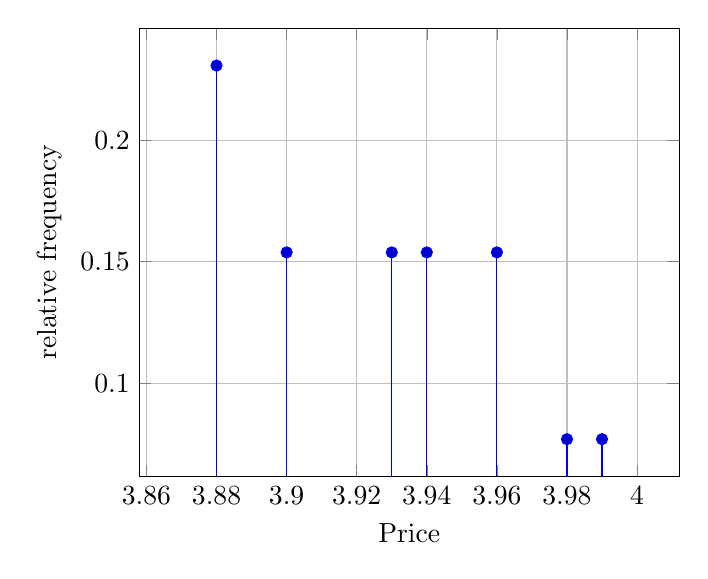
\begin{tikzpicture}
			\begin{axis}[enlarge x limits=0.2, grid = both,
				xlabel = Price, ylabel = relative frequency] 
				\addplot+[ycomb] plot coordinates {(3.88, 3/13) (3.94, 2/13) (3.90, 2/13) (3.96, 2/13) (3.93, 2/13) (3.99, 1/13) (3.98, 1/13)};  
			\end{axis} 
		\end{tikzpicture}
	\end{figure}
	
	\item A pie chart uses the relative frequency of a data entry to allot the sector angle as a proportion of the full 360 degree circle. The sector angle would be $ \theta_i = 360 \times r_i $.
	
	\item Pie chart uses the relative frequencies of the 4 entries.
	\begin{table}[H]
		\centering
		\begin{tabular}{@{}lll@{}}
			\toprule
			Country       & Oil Reserve & Fraction Oil        \\ \midrule
			United States & 38.7        & 0.30  \\
			South America & 22.6        & 0.17 \\
			Canada        & 8.8         & 0.07  \\
			Mexico        & 60.0        & 0.46  \\ \bottomrule
		\end{tabular}
	\end{table}
	
	\begin{figure}[H]
		\centering
		\caption{Pie chart displaying Oil Reserve percentages}
		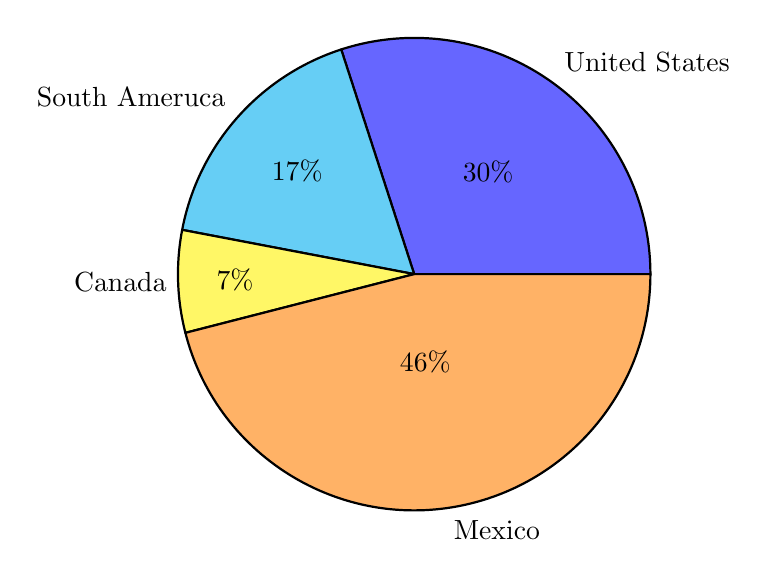
\begin{tikzpicture}
			\pie{30/United States,
				17/South Ameruca,
				7/Canada,
				46/Mexico}
		\end{tikzpicture}
	\end{figure}
	
	
	\item The two histograms generated using the first 1000 sentences of two distinct passages are as follows : \\
	
	\begin{figure}[H]
		\centering
		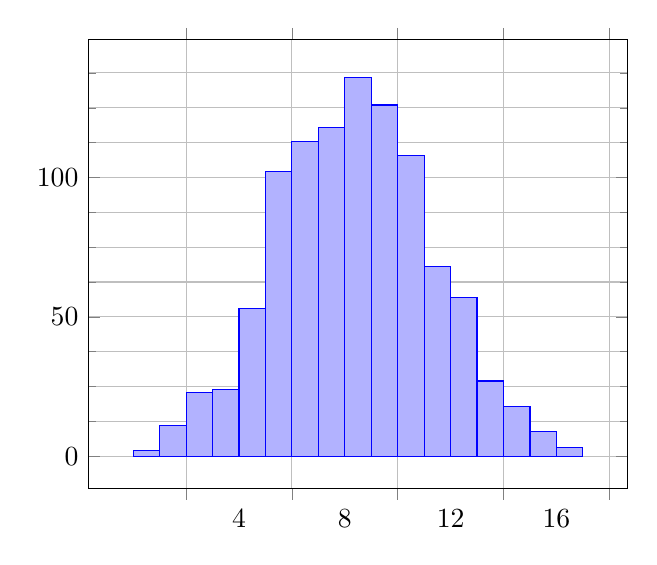
\begin{tikzpicture}
			\begin{axis}[ybar interval, minor y tick num = 3, grid = both, xtick = {0, 4, 8, 12, 16, 20}]
				\addplot coordinates { (2.0, 2)
					(3.0, 11)
					(4.0, 23)
					(5.0, 24)
					(6.0, 53)
					(7.0, 102)
					(8.0, 113)
					(9.0, 118)
					(10.0, 136)
					(11.0, 126)
					(12.0, 108)
					(13.0, 68)
					(14.0, 57)
					(15.0, 27)
					(16.0, 18)
					(17.0, 9)
					(18.0, 3)
					(19.0, 2) };
			\end{axis}
		\end{tikzpicture}
	\end{figure}
	
	
	\begin{figure}[H]
		\centering
		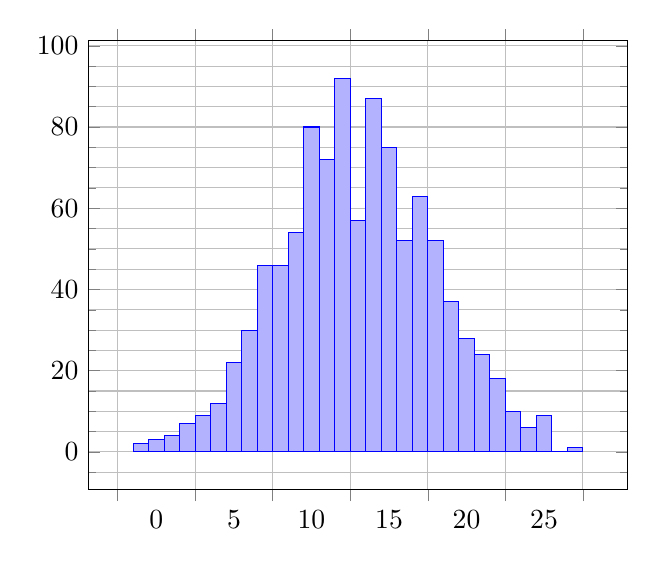
\begin{tikzpicture}
			\begin{axis}[ybar interval, minor y tick num = 3, grid = both, xtick = {0, 5, 10, 15, 20, 25, 30}]
				\addplot coordinates { (1.0, 2)
					(2.0, 3)
					(3.0, 4)
					(4.0, 7)
					(5.0, 9)
					(6.0, 12)
					(7.0, 22)
					(8.0, 30)
					(9.0, 46)
					(10.0, 46)
					(11.0, 54)
					(12.0, 80)
					(13.0, 72)
					(14.0, 92)
					(15.0, 57)
					(16.0, 87)
					(17.0, 75)
					(18.0, 52)
					(19.0, 63)
					(20.0, 52)
					(21.0, 37)
					(22.0, 28)
					(23.0, 24)
					(24.0, 18)
					(25.0, 10)
					(26.0, 6)
					(27.0, 9)
					(28.0, 0)
					(29.0, 1)
					(30.0, 1)};
			\end{axis}
		\end{tikzpicture}
	\end{figure}
	
	No, this would not be sufficient as the distribution always tends to be approximately normal.
	
	\item The number of days is the sum of all frequencies $ \sum f_i  = 33$.
	The sum of all travel times is the weighted sum of the travel times. $  \sum x_i f_i  = 767 $ \\
	
	\item \begin{enumerate}
		\item The frequency table extracted from the given data is :
		\begin{figure}[H]
			\begin{subfigure}[]{0.45\linewidth}
				\centering
				\begin{table}[H]
					
					\begin{tabular}{@{}rr@{}}
						\toprule
						Accidents & Frequency \\ \midrule
						0         & 1         \\
						1         & 3         \\
						2         & 6         \\
						3         & 4         \\
						4         & 5         \\
						6         & 2         \\
						11        & 1         \\ \bottomrule
					\end{tabular}
				\end{table}
			\end{subfigure}
			%
			\begin{subfigure}[]{0.45\linewidth}
				\centering
				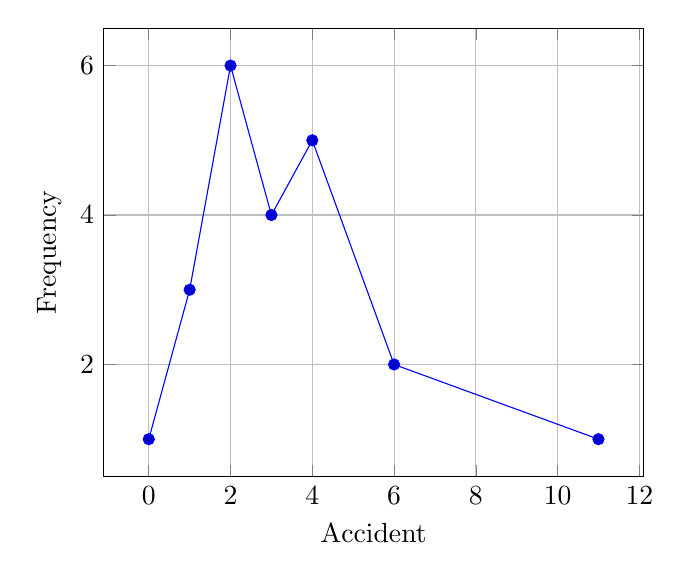
\begin{tikzpicture}
					\begin{axis}[grid = both, xlabel = Accident, ylabel = Frequency]
						\addplot coordinates { (0, 1) (1, 3) (2, 6) (3, 4) (4, 5) (6, 2) (11, 1)};
					\end{axis}
				\end{tikzpicture}
			\end{subfigure}
			
		\end{figure}
		
		\item The frequency polygon is shown above.
		
		\item Cumulative relative frequency plot is below \\
		
		\begin{figure}[H]
			\centering
			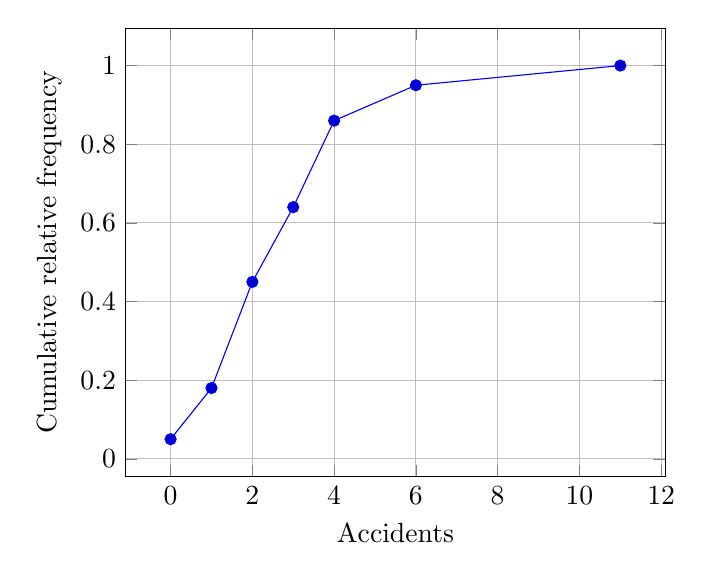
\begin{tikzpicture}
				\begin{axis}[grid = both, xlabel = Accidents, ylabel = Cumulative relative frequency]
					\addplot coordinates {(0, 0.05) (1, 0.18) (2, 0.45) (3, 0.64) (4, 0.86) (6, 0.95) (11, 1.0)};
				\end{axis}
			\end{tikzpicture}
		\end{figure}
		
		\item Mean = 3.18. Median = 3. Mode = 2. Standard Deviation = 2.32.
		
		
	\end{enumerate}
	
	\item \begin{enumerate}
		\item The histogram of fatalities is below.
		\begin{figure}[H]
			\centering
			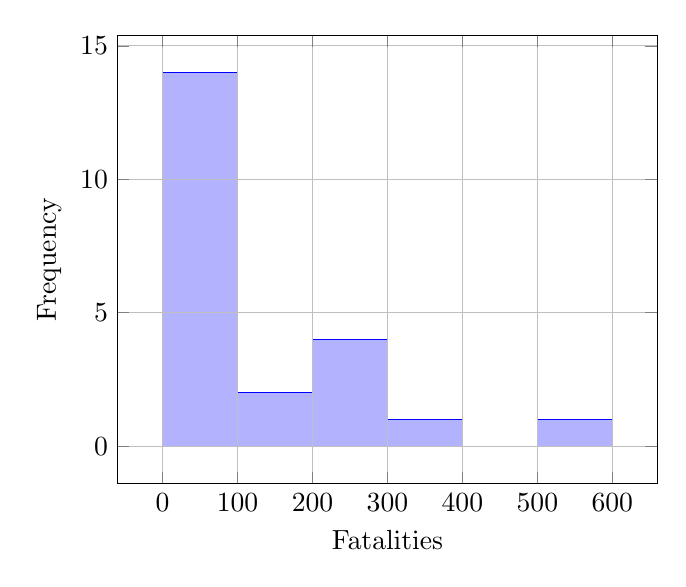
\begin{tikzpicture}
				\begin{axis}[grid = both, xtick = {0, 100, 200, 300, 400, 500, 600, 700}, area style,
					xlabel = Fatalities, ylabel = Frequency]
					\addplot+[ybar interval, mark = no] plot coordinates { (0, 14) (100, 2) (200, 4) (300, 1) (400, 0) (500, 1) (600, 0) };
				\end{axis}
			\end{tikzpicture}
		\end{figure}
		
		\item Stem and leaf plot is just a worse histogram. Ignored.
		\item Mean = 119.14. Median = 3. Mode = 44.5. Standard Deviation = 144.8
	\end{enumerate}
	
	\item Let $ \{x_1\} , \{x_2\} $ be the women and $ \{y_1\} , \{y_2\} $ be the men with means $ \bar{x_1}, \bar{x_2}, \bar{y_1}, \bar{y_2} $ respectively. Given that $ a $ is for all adults,
	
		\begin{align}
			\overline{x_1} > \overline{x_2} &\qquad \text{and} \qquad \overline{y_1} > \overline{y_2} \\
			%
			\overline{x_1 + y_1} &= \overline{x_1} + \overline{y_1} \\
			%
			\overline{x_1} + \overline{y_1} &> \overline{x_2} + \overline{y_2} \\
			%
			\overline{x_1 + y_1} &> \overline{x_2 + y_2} \\
			%
			\overline{a_1} &> \overline{a_2}
		\end{align}
		
		The above holds true for real world populations with an almost equal number of men and women. Consider the special case with a fraction $ p $ of the town being male. 
		\begin{align}
			\overline{a_1} &= p_1 \overline{y_1} + (1 - p_1) \overline{x_1} \\
			%
			\overline{a_2} &= p_2 \overline{y_2} + (1 - p_2) \overline{x_2} \\
		\end{align}
		
		It is easy to see that when $ p_1 << p_2 $, but the male and female weight averages are only slightly different between towns A and B, $ a_1 < a_2 $ is possible.
		
	
	\item Benford's Law in table and graph form : 
	\begin{figure}[H]
		\begin{subfigure}[]{0.45\linewidth}
			\centering
			\begin{table}[H]
				\centering
				\begin{tabular}{@{}rr@{}}
					\toprule
					First digit &  Proportion of data \\
					\midrule
					1 &               0.301 \\
					2 &               0.176 \\
					3 &               0.125 \\
					4 &               0.097 \\
					5 &               0.079 \\
					6 &               0.067 \\
					7 &               0.058 \\
					8 &               0.051 \\
					9 &               0.046 \\
					\bottomrule
				\end{tabular}
			\end{table}
		\end{subfigure}
		%
		\begin{subfigure}[]{0.45\linewidth}
			\centering
			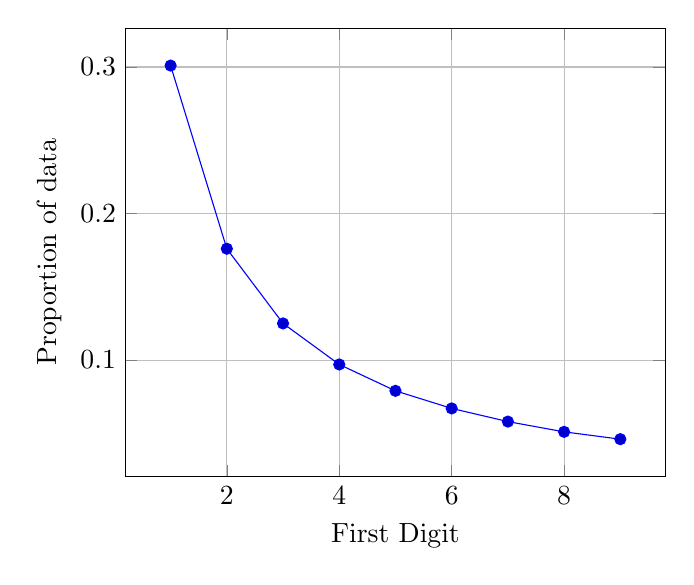
\begin{tikzpicture}
				\begin{axis}[grid = both, xlabel = First Digit, ylabel = Proportion of data]
					\addplot coordinates { (1, 0.301) (2, 0.176) (3, 0.125) (4, 0.097) (5, 0.079) (6, 0.067) (7, 0.058) (8, 0.051) (9, 0.046)};
				\end{axis}
			\end{tikzpicture}
		\end{subfigure} \\		
	\end{figure}
	
	Benford's law would make the option c = 1.4512 the best guess.
	
	\item Let the total employee payrolls be $ A_1 $ and $ A_2 $. Then, 
	
		\begin{align}
			\overline{x_1} = A_1 / 100 \quad &\text{and} \quad \overline{x_2} = A_2 / 110 \\
			%
			A_1 > A_2 \quad &\implies \quad A_1 / 100 > A_2 / 100 > A_2 / 110 \\
			%
			\overline{x_1} &> \overline{x_2} 
		\end{align}
	
	
	No comment can be made about the comparison between medians.
	
	\item Let the first half dataset be $ \{x_i\} $ and the second half be $ \{y_i\} $, now : 
	\begin{enumerate}
		\item Mean of the first and second half is $\overline{x}$ and $ \overline{y} $, both with same number of elements $ n $. Mean of combined dataset is : 
		\begin{align}
			\overline{z} = \frac{\sum_{i} x_i + \sum_{i} y_i}{n + n} = \frac{\overline{x} + \overline{y}}{2} = 110
		\end{align}
		
		\item Median of the combined dataset has to lie between the medians of the first and second halves. $ 100 \leq \text{Median}  \leq 120 $. This assumes that the dataset is sorted before being split into halves.
		
		\item No comment can be made about the mode.
	\end{enumerate}
	
	\item Using the midpoints of the class intervals
	\begin{table}[H]
		\centering
		\begin{tabular}{rrrrr}
			\toprule
			StartAge &  EndAge &  Males &  Females &  MidAge \\
			\midrule
			0 &       5 &    120 &       67 &     2.5 \\
			5 &      10 &    184 &      120 &     7.5 \\
			10 &      15 &     44 &       22 &    12.5 \\
			15 &      20 &     24 &       15 &    17.5 \\
			20 &      30 &     23 &       25 &    25.0 \\
			30 &      40 &     50 &       22 &    35.0 \\
			40 &      50 &     60 &       40 &    45.0 \\
			50 &      60 &    102 &       76 &    55.0 \\
			60 &      70 &    167 &      104 &    65.0 \\
			70 &      80 &    150 &       90 &    75.0 \\
			80 &     100 &     49 &       27 &    90.0 \\
			\bottomrule
		\end{tabular}
	\end{table}
	
	\begin{enumerate}
		\item Mean for males = 40.904  and Mean for females = 40.98\\
		\item Median is calculated by finding the class interval containing the middle term and then linearly interpolating within that interval. A similar process is used to find the quartiles.
		
		The quartiles for males are 8.3, 47 and 67.3.
		The quartiles for females are 8.5, 48.2 and 66.6.
	\end{enumerate}
	
	\item Using the formulas in the text, mean =  15.7, standard deviation = 4.4.
	
	\item Given that $ n = 5 $, $ \overline{x} = 104 $ and $ s^2 = 16 $, 
	
	
		\begin{align}
			104 &= \frac{ 102 + 100 + 105 + x_{4} + x_{5} }{5} \\
			%
			x_4 + x_5 &= 213 \\
			%
			16 * (5 - 1) &= (102)^2 + (100)^2 + (105)^2 + (x_4)^2 + (x_5)^2  - (5)(104)^2 \\
			%
			(x_4)^2 + (x_5)^2 &= 22715
		\end{align}
		
		This is a quadratic system of equations with the solution $ x_4 = 110.4 $ and $ x_5 = 102.6 $.
	
	
	\item No. The additional information needed is the population of all the states. This will be used to weight the mean salaries of the individual states to calculate the national average.
	
	\item Mean = 127.425, Std Dev = 11.87, Median = 127.5, Mode = 132.5 (using bin size 5).
	The cumulative frequency graph is as follows : 
	
	
	\item Sample mean = 18.9, Median = 19.3, Mode = 21.2, Variance =  6.25\\
	\begin{figure}[H]
		\centering
		
	\end{figure}
	
	\begin{figure}[H]
		\begin{subfigure}[]{0.45\linewidth}
			\centering
			\begin{table}[H]
				\centering
				\begin{tabular}{rr}
					\toprule
					Midpoints &  Frequency \\
					\midrule
					13.5 &          2 \\
					14.5 &          2 \\
					15.5 &          3 \\
					16.5 &          4 \\
					17.5 &          6 \\
					18.5 &          7 \\
					19.5 &          6 \\
					20.5 &         10 \\
					21.5 &          5 \\
					22.5 &          1 \\
					23.5 &          4 \\
					\bottomrule
				\end{tabular}
			\end{table}
		\end{subfigure}
		%
		\begin{subfigure}[]{0.45\linewidth}
			\centering
			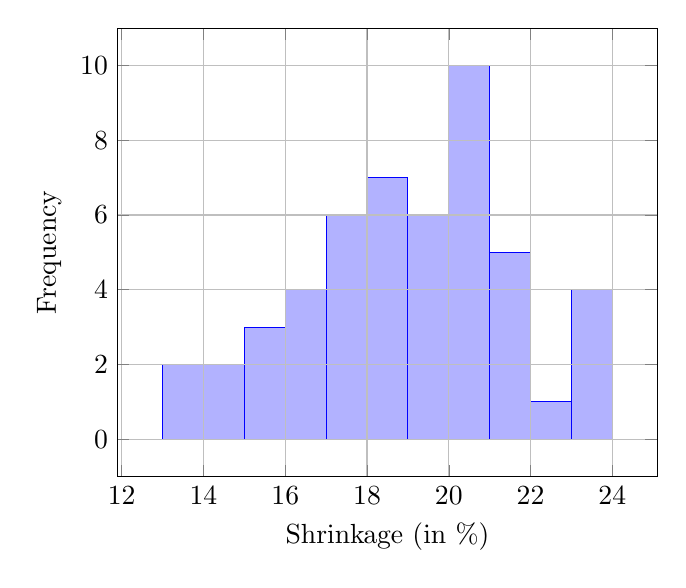
\begin{tikzpicture}
				\begin{axis}[grid = both, xlabel = Shrinkage (in \%), ylabel = Frequency, area style]
					\addplot+[ybar interval, mark = no] plot coordinates {(13, 2) (14, 2) (15, 3) (16, 4) (17, 6) (18, 7) (19, 6) (20, 10) (21, 5) (22, 1) (23, 4) (24, 0)};
				\end{axis}
			\end{tikzpicture}
		\end{subfigure} \\		
	\end{figure}
	
	Using the table with midpoints above, Mean = 18.98, Variance = 6.53. They differ from the actual mean and variance above because of the binning approximations.
	
	\item The recursive mean formula can be proved using : 
	
	
		\begin{align}
			\overline{x}_{j + 1} &= \frac{1}{j + 1} \sum\limits_{i = 1}^{j + 1} x_{i} \\
			%
			& = \frac{j}{j + 1} \left( \frac{1}{j} \sum\limits_{i = 1}^{j} x_{i} \right) + \frac{x_{j + 1}}{j + 1} \\
			%
			& = \left( 1 - \frac{1}{j + 1} \right) \overline{x}_{j} + \frac{x_{j + 1}}{j + 1} \\
			%
			& = \overline{x}_{j} + \frac{x_{j + 1} - \overline{x}_{j}}{j + 1}
		\end{align}
	 \\
	
	Using the normal method, mean = 5.16 and variance = 6.96.
	Using the recursive formula, mean = 5.16 and variance = 6.96. They match.
	
	\item The 90 percentile for January averages is 46 degrees.
	The 75 percentile for January averages is 70.45 degrees.
	
	\item The quartiles are 74, 85, 91.5.
	
	\item Mean = 84.92, variance = 928.63.
	Quartiles are 60.25, 95.5, 113.25.
	
	\item ... larger than all of the existing values.
	
	\item The box plot representing the data is as follows : \\
	
	\begin{figure}[H]
		\centering
		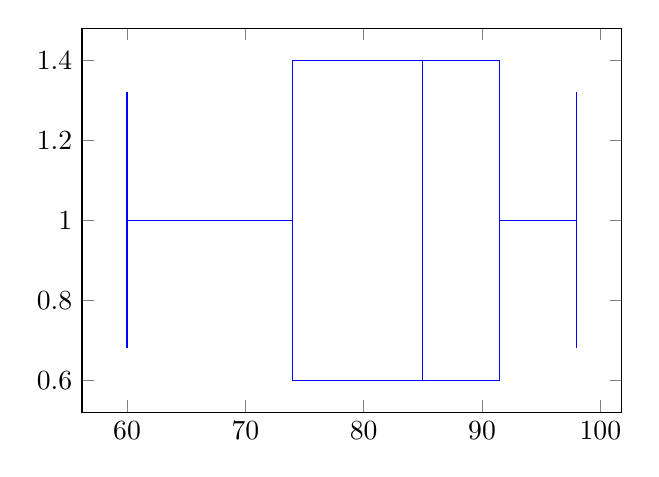
\begin{tikzpicture}
			\begin{axis}[
				y=2in,
				]
				\addplot+ [
				boxplot prepared={
					lower whisker=60,
					lower quartile=74,
					median=85,
					upper quartile=91.5,
					upper whisker=98,
				},
				]
				table [row sep=\\,y index=0] {
					data\\
				};
			\end{axis}
		\end{tikzpicture}
	\end{figure}
	
	\item The data is shown as a histogram as follows. It is not a normal distribution.
	
	\begin{figure}[H]
		\centering
		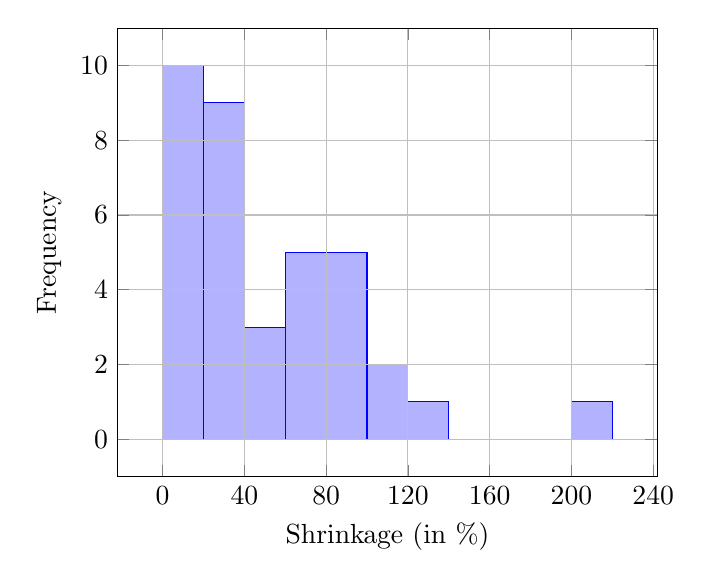
\begin{tikzpicture}
			\begin{axis}[grid = both, xlabel = Shrinkage (in \%), ylabel = Frequency, area style,
				xtick = { 0,  40,  80, 120, 160, 200, 240}]
				\addplot+[ybar interval, mark = no] plot coordinates { (0, 10) (20, 9) (40, 3) (60, 5) (80, 5) (100, 2) (120, 1) (140, 0) (160, 0) (180, 0) (200, 1) (220, 0) };
			\end{axis}
		\end{tikzpicture}
	\end{figure} 
	
	
	\item Mean = 0.35, Median = 0.35, Standard Deviation = 0.117, with the histogram looking approximately normal.
	37 of 55 values (67 \%) are within 1 std of the mean.
	
	\begin{figure}[H]
		\centering
		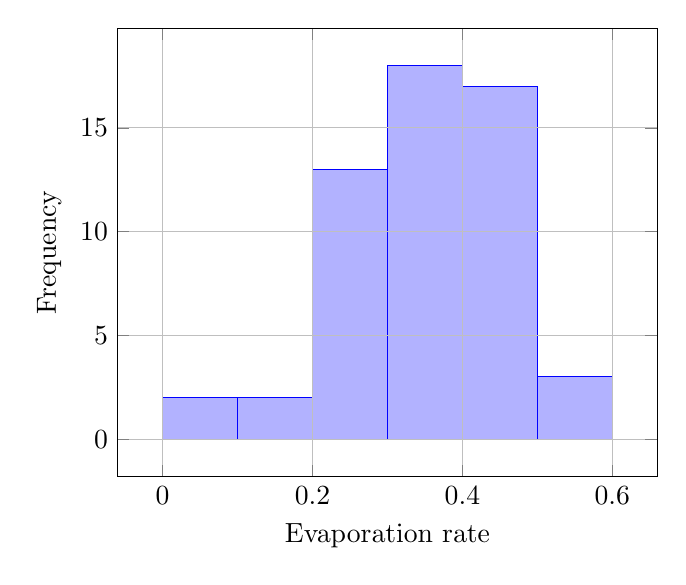
\begin{tikzpicture}
			\begin{axis}[grid = both, xlabel = Evaporation rate, ylabel = Frequency, area style,
				xtick = {0, 0.2, 0.4, 0.6, 0.8}]
				\addplot+[ybar interval, mark = no] plot coordinates { (0.0, 2) (0.1, 2) (0.2, 13) (0.3, 18) (0.4, 17) (0.5, 3) (0.6, 0)};
			\end{axis}
		\end{tikzpicture}
	\end{figure} 
	
	\item \begin{enumerate}
		\item Mean = 3.72, std dev = 0.146.
		
		
		\item 80\% of entries are within 1.5 std dev of the mean. Chebyshev inequality lower limit is 55.6 \%.
		\item 100\% of entries are within 2 std dev of the mean. Chebyshev inequality lower limit is 75 \%.
		\item Stem and leaf plot is replaced by histogram here.
		
		\begin{figure}[H]
			\centering
			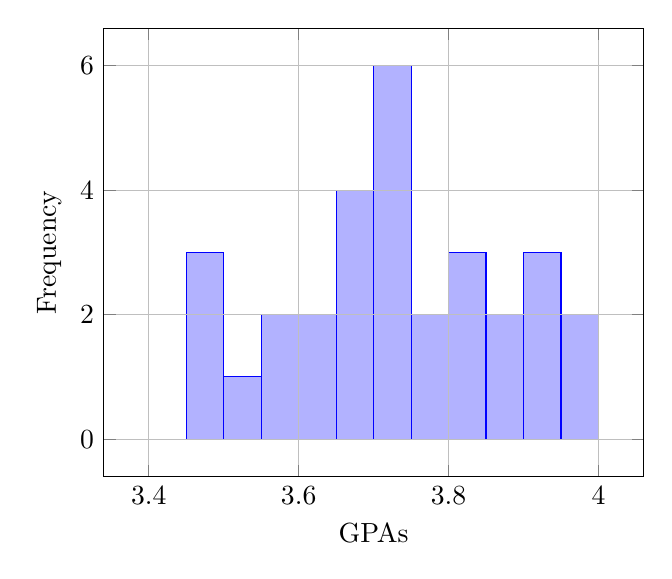
\begin{tikzpicture}
				\begin{axis}[grid = both, xlabel = GPAs, ylabel = Frequency, area style,
					xtick = {3.2, 3.4, 3.6, 3.8, 4.0, 4.2}]
					\addplot+[ybar interval, mark = no] plot coordinates { (3.4, 0) (3.45, 3) (3.5, 1) (3.55, 2) (3.6, 2) (3.65, 4) (3.7, 6) (3.75, 2) (3.8, 3) (3.85, 2) (3.9, 3) (3.95, 2) (4.0, 0)};
				\end{axis}
			\end{tikzpicture}
		\end{figure} 
		
		
	\end{enumerate}
	
	\item The approximate Chebyshev limits do not match the actual proportions. This is because the dataset is not normally distributed.
	
	The empirical value numbers are calculated using the area under the curve of a standard normal distribution in the interval [$ -k, k $] in order to find the fraction of data points in the interval [$ \mu - k \sigma, \mu + k \sigma $] \\
	
	The empirical rule dictates that the fraction of data points within 1.5 std dev of the mean is 86.6 \%, compared to observed value of 80 \% \\
	The empirical rule dictates that the fraction of data points within 2 std dev of the mean is 95 \%, compared to observed value of 100 \% \\
	
	\item No, because the health club consists of members of the total population who are above average weight. 
	
	\item \begin{enumerate}
		\item Mean = 127.425, Median = 127.5.
		
		\item A histogram of the data to check if it is normal : yes it is.
		
		\begin{figure}[H]
			\centering
			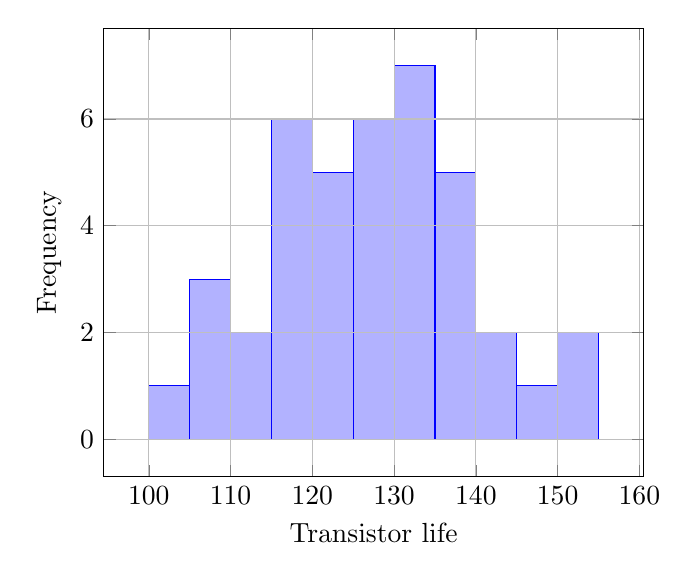
\begin{tikzpicture}
				\begin{axis}[grid = both, xlabel = Transistor life, ylabel = Frequency, area style]
					\addplot+[ybar interval, mark = no] plot coordinates {(100, 1) (105, 3) (110, 2) (115, 6) (120, 5) (125, 6) (130, 7) (135, 5) (140, 2) (145, 1) (150, 2) (155, 0)};
				\end{axis}
			\end{tikzpicture}
		\end{figure} 
		
		\item Standard Deviation = 11.87.
		
		\item The empirical rule dictates that the fraction of data points within 1.5 std dev of the mean is 86.6 \%, compared to observed value of 85 \%.
		
		\item The Chebyshev minimum fraction is 55.6 \% of data within 1.5 std dev of the mean. This rule is obeyed.
	\end{enumerate}
	
	\item Sample correlation coefficient is r = 0.484 \\
	
	\begin{figure}[H]
		\centering
		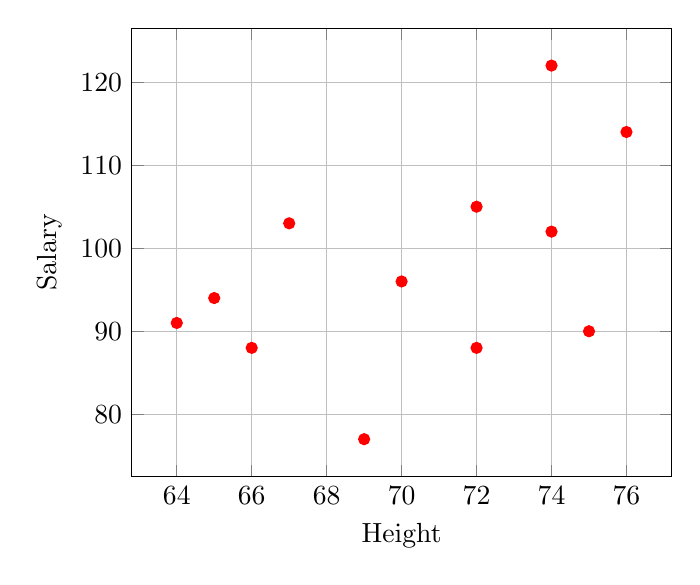
\begin{tikzpicture}
			\begin{axis}[grid = both, xlabel = Height, ylabel = Salary]
				\addplot[only marks, color = red] coordinates {(64, 91) (65, 94) (66, 88) (67, 103) (69, 77) (70, 96) (72, 105) (72, 88) (74, 122) (74, 102) (75, 90) (76, 114)
				};
			\end{axis}
		\end{tikzpicture}
	\end{figure}
	
	\item No causation can be declared from the correlation. It is possible that the good posture is a result of trying to relieve the back pain.
	
	\item No. A possible explanation is that immigrants tend to settle down in higher-paying states.
	
	\item r = 0.743 between Hours studied and GPA.
	
	\item 	Verifying property 3 of sample correlation coefficient : 
	
	
		\begin{align}
			y_i \ &=\  a + b x_i \qquad \text{with} \qquad b < 0 \\
			%
			s_{y}^{2} \ &=\ b^2 s_{x}^2 \\
			%
			r \ &=\ \frac{\sum_{i} (x_i - \bar{x}) (y_i - \bar{y})}{(n - 1) s_x s_y} \\
			%
			r \ &=\ \frac{b \sum_{i} (x_i - \bar{x})^{2}}{- b (n - 1) s_{x}^{2}} \\
			%
			r &= -1			
		\end{align}
	\\
	
	\item Verifying property 4 : 
	
	
		\begin{align}
			p_i \ &=\  a + b x_i \qquad q_i \ =\  c + d y_i \qquad \text{with} \qquad bd > 0 \\
			%
			s_{p}^{2} \ &=\ b^2 s_{x}^2 \qquad \text{and} \qquad s_{q}^{2} \ =\ d^2 s_{y}^2 \\
			%
			r_{pq} \ &=\ \frac{\sum_{i} (p_i - \bar{p}) (q_i - \bar{q})}{(n - 1) s_p s_q} \\
			%
			r_{pq} \ &=\ \frac{bd \sum_{i} (x_i - \bar{x}) (y_i - \bar{y})}{|bd| (n - 1) s_{x} s_{y}} \\
			%
			r_{pq} &= r_{xy} \qquad \text{if} \qquad bd > 0			
		\end{align}
	\\
	
	\item Grades 2-4 imply children with a range of ages, so height is less likely to be directly causing the higher reading scores  compared to age itself.
	
	\item Family wealth, nurture and the emphasis it places on early literacy, school environments and peer group are all possible confounding factors that are extremely difficult to adjust for.
	
	\item The Lorenz curve is as follows, with Gini Index = 0.1567.
	
	\begin{figure}[H]
		\centering
		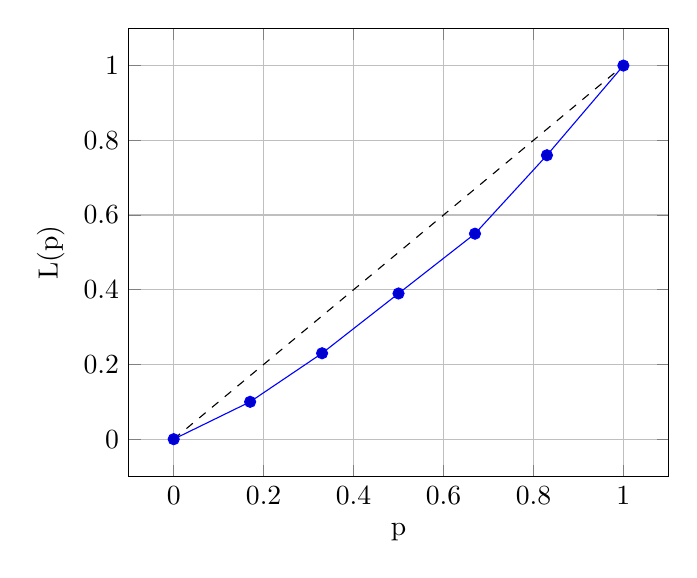
\begin{tikzpicture}
			\begin{axis}[grid = both, xlabel = p, ylabel = L(p)]
				\addplot coordinates {(0.0, 0.0) (0.17, 0.1) (0.33, 0.23) (0.5, 0.39) (0.67, 0.55) (0.83, 0.76) (1.0, 1.0)
				};
				\draw[dashed] (axis cs:0, 0) -- (axis cs:1, 1);
			\end{axis}
			
		\end{tikzpicture}
	\end{figure} 
	
	\item The Lorenz curve is as follows, with Gini Index = 0.163.
	
	\begin{figure}[H]
		\centering
		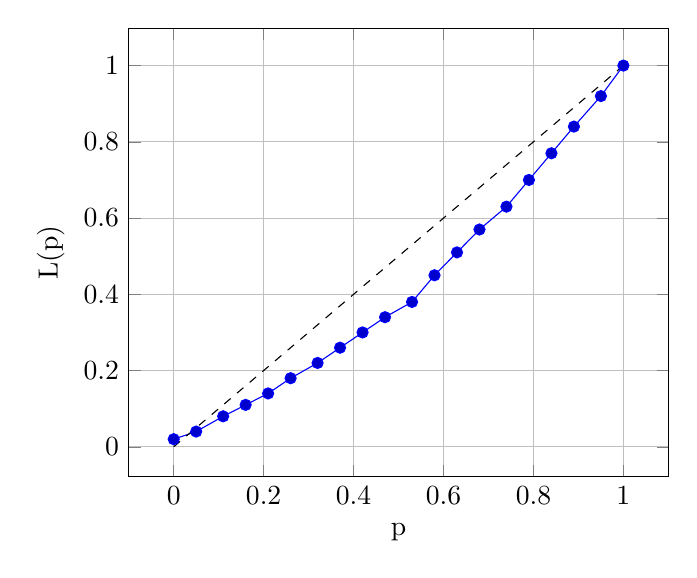
\begin{tikzpicture}
			\begin{axis}[grid = both, xlabel = p, ylabel = L(p)]
				\addplot coordinates {(0.0, 0.02) (0.05, 0.04) (0.11, 0.08) (0.16, 0.11) (0.21, 0.14) (0.26, 0.18) (0.32, 0.22) (0.37, 0.26) (0.42, 0.3) (0.47, 0.34) (0.53, 0.38) (0.58, 0.45) (0.63, 0.51) (0.68, 0.57) (0.74, 0.63) (0.79, 0.7) (0.84, 0.77) (0.89, 0.84) (0.95, 0.92) (1.0, 1.0)
				};
				\draw[dashed] (axis cs:0, 0) -- (axis cs:1, 1);
			\end{axis}
			
		\end{tikzpicture}
	\end{figure} 
	
	\item From the formula for the Lorenz curve data points, multiplying all data by a constant has no effect as it cancels out.
	Adding a positive constant to every data point, makes some Lorenz values larger and some smaller. So, the effect on the Gini index cannot be predicted.
	
\end{enumerate}


%	\chapter{Elements of Probability}

\begin{enumerate}
	\item With replacement, there are 9 elements in the sample space, since the first and second marble can be any of the 3 colors. $ S = \{ x_i, x_j \} $, where $ i, j = \{ r, b, g \} $. 9 possible permutations.
	
	Without replacement, the sample space is $ S = \{ x_i, x_j \} $, where $ j \neq i $.
	
	\begin{align}
		\text{permutations without replacement} =  \binom{3}{1} \ \binom{2}{1} \ = \ 6
	\end{align}
	
	\item Three coin tosses result in $ 2^3  = 8$ possible permutations. The subset of the sample space corresponding to more heads than tails is $ \{ hht, hth, thh, hhh \} $.
	
	\item 	
		\begin{align}
			E F &= \{ 7 \} \\
			%
			E \cup FG &= \{ 1, 3, 4, 5, 7 \} \\
			%
			E G^\complement &= \{ 3, 5, 7 \} \\
			%
			E F^\complement \cup G &= \{ 1, 3, 4, 5 \} \\
			%
			E^\complement \  ( F \cup G ) &= \{ 4, 6 \} \\
			%
			EG \cup FG &= (E \cup F) \ G = \{ 1, 4 \}
		\end{align}	
	
	
	\item \begin{enumerate}
		\item First die lands on 1 and sum of dice is odd. $ EF  = \{ (1,2), (1,4), (1,6) \}$.
		
		\item First die lands on 1 or sum of dice is odd. $ E \cup F = \{ (1, n) $ and the other 15 possibilities are $ (3, \text{even}), (5, \text{even}), (2, \text{odd}), (4, \text{odd}), (6, \text{odd}) \} $ \\
		
		\item First die lands on 1 and sum is 5. $ FG = \{ (1,4) \} $ \\
		
		\item Sum of dice is odd and first die does not land on 1. 15 elements.
		\begin{align}
			E F^\complement = \{ (2, \text{odd}), (4, \text{odd}) , (6, \text{odd}), (3, \text{even}), (5, \text{even})\} 
		\end{align}
		
		\item $ EFG = \{ (1, 4) \} = FG $
	\end{enumerate} 
	
	\item \begin{enumerate}
		\item $ 2^4 = 16 $ possibilities.
		
		\item System works = $ \{ (1,1,0,0), (1,1,0,1), (1,1,1,0), (1,1,1,1)\} $ and the other branch is
		$ \{ (0,0,1,1), (1,0,1,1), (0,1,1,1) \} $ \\
		
		\item 4 permutations of component 2 and 4 gives 4 outcomes.
	\end{enumerate}
	
	\item 
		\begin{align}
			E F^\complement G^\complement \\
			%
			E G F^\complement \\
			%
			E \cup F \cup G \\
			%
			EF \cup FG \cup EG \\
			%
			EFG \\
			%
			E ^\complement F^\complement G^\complement \\
			%
			(EF \cup FG \cup EG )^\complement \\
			%
			( EFG )^\complement \\
			%
			( EF G^\complement) \cup (FG E^\complement) \cup (EG F^\complement) \\
			%
			S
		\end{align}
	
	
	\item 
		\begin{align}
			E \cup E^\complement &= S \\
			%
			E E^\complement &= \varnothing \\
			%
			(E \cup F)\ (E \cup F^\complement) &= EE \cup EF \cup EF^\complement \cup FF^\complement = E \\
			%
			(E \cup F)\ (E \cup F^\complement) (E^\complement \cup F) &= E\ (E^\complement \cup F) = EF \\
			%
			(E \cup F)\ (F \cup G) &= EF \cup FF \cup FG \cup EG = F \cup EG
		\end{align}
	
	
	\item \begin{enumerate}
		
		\item If $ x \in E $ and $ x \in F $, then $ x \in E \ \forall\  x $. Thus, $ EF \subset E $.
		If $ x \in E $, then $ x \in E $ or $ x \in F $ is true $ \forall \ x $. Thus $ E \subset (E \cup F) $.
		
		\item If $ x \in E $, then $ x \in F \ \forall \ x$.
		If  $ y \in F^\complement $, then $ y \in E^\complement $ is true $ \forall \ y $, using $ E \subset F $. Thus, $ F^\complement \subset E^\complement $ \\
		
		\item If $ x \in (E \cup F) \ \forall\ x$, then $ x \in E $ or $ x \in F $ is true $ \forall \ x $.
		$ x \in (F \cup E) \ \forall\ x$. This proves the commutative law for unions.
		
		If $ x \in (E F) \ \forall\ x$, then $ x \in E $ and $ x \in F $ is true $ \forall \ x $.
		$ x \in (F  E) \ \forall\ x$. This proves the commutative law for intersections.
		
		\item If $ x \in E $ or $ x \in F $ or $ x \in G $ is true $ \forall \ x $, then \\
		$ x \in (E \cup F) \cup G \quad \forall \ x$ as well as $ x \in E(\cup (F \cup G) \quad \forall \ x$.
		This proves the associative law for unions.
		
		If $ x \in E $ and $ x \in F $ and $ x \in G $ is true $ \forall \ x $, then \\
		$ x \in (E F) \cap G \quad \forall \ x$ as well as $ x \in E \cap (F G) \quad \forall \ x$.
		This proves the associative law for intersections.
		
		\item $ FE \cup FE^\complement $ can be simplified using the above laws into \\
		$ F (E \cup E^\complement) = F S = F$ \\
		
		\item $ F = F (E \cup E^\complement) $, using this in the left hand side,
		$ E \cup FE \cup FE^\complement = E \cup F E^\complement$ \\
		
		\item If $ x \in (E \cup F)^\complement $, then $ x \notin E $ and $ x \notin F  \quad \forall \ x$.
		Now, $ x \in E^\complement $ and $ x \in F^\complement  \quad \forall \ x$. Thus, $ x \in E^\complement F^\complement \quad \forall \ x $ \\
		This means that $ (E \cup F)^\complement \subset E^\complement F^\complement $.
		
		If $ y \in E^\complement F^\complement $, then $ y \notin E $ and $ y \notin F \quad \forall \ y$.
		Then, $ y \notin (E \cup F) $ and therefore, $ y \in (E \cup F)^\complement \quad \forall \ y$.
		This means that $  E^\complement F^\complement \subset (E \cup F)^\complement $.
		
		If $ z \in (EF)^\complement $, then $ z \notin EF \quad \forall \ z$.
		Then, $ z \in E^\complement$ or $ z \in F^\complement $ and therefore, $ z \in E^\complement \cup F^\complement \quad \forall \ z$.
		This means that $  (EF)^\complement \subset E^\complement \cup F^\complement $.
		
		If $ w \in E^\complement \cup F^\complement $, then $ w \notin E $ or $ w \notin F \quad \forall \ w$.
		Then, $ w \notin EF $ and therefore, $ w \in (EF)^\complement  \quad \forall \ w$.
		This means that $ E^\complement \cup F^\complement \subset (EF)^\complement$.
		
		Using the fact that two sets which are subsets of each other are identical, De-Morgan's laws are proved.
		
	\end{enumerate}
	
	\item 
		\begin{align}
			I &= E F^\complement G^\complement \\
			%
			II &= E F G^\complement \\
			%
			III &= E^\complement F G^\complement \\
			%
			IV &= EFG \\
			%
			V &= E^\complement F G \\
			%
			VI &= E^\complement F^\complement G \\
			%
			VII &= E F^\complement G
		\end{align}
	\\
	
	\item $ F = FE \cup F E^\complement $ where $ FE \cap F E^\complement = \varnothing $.
	Given $ E \subset F $, $ FE = E $ follows. Now, $ F = E \cup F E^\complement $.
	This proves $ P(F) \geq P(E) $.
	
	\item Boole's inequality for two events : 
	
		\begin{align}
			P(E_1 \cup E_2) &= P(E_1) + P(E_2) - P(E_1 E_2)\\
			%
			& \leq P(E_1) + P(E_2)
		\end{align}
		
		Extending to more than two events,
		
		\begin{align}
			P \left( \bigcup_{i = 1}^{n} E_i \right) &= \sum\limits_{i = 1}^{n} P(E_i) \ - \ P(\text{area counted more than once}) \\
			%
			P \left( \bigcup_{i = 1}^{n} E_i \right) &\leq \sum\limits_{i = 1}^{n} P(E_i)
		\end{align}
	\\
	
	\item Bonferroni's inequality : 
	
		\begin{align}
			P(E) + P(F) - P(EF)  &= P(E \cup F) \\
			%
			E \cup F &\in S\\
			%
			P(E \cup F) &\leq 1 \\
			%
			P(E) + P(F) - P(EF) &\leq 1 \\
			%
			P(EF) &\geq P(E) + P(F) - 1
		\end{align}
	 \\
	
	\item	\begin{enumerate}
		\item 
		
		
			\begin{align}
				P(E F^\complement) &= P(E) + P(F^\complement) - P(E \cup F^\complement) \\
				%
				&= P(E) - (P(E \cup F^\complement) - P(F^\complement)) \\
				%
				P(E \cup F^\complement) &= 1 - (P(F) - P(EF)) \\
				%
				P(F^\complement) &= 1 - P(F) \\
				%
				P(E F^\complement) &= P(E) + 1 - P(F) - 1 +  P(F) - P(EF) \\
				%
				P(E F^\complement) &= P(E) - P(EF)
			\end{align}
			\item 
			\begin{align}
				P(E^\complement F^\complement) &= P(E^\complement) + P(F^\complement) - P(E^\complement \cup F^\complement) \\
				%
				&= 1 - P(E) + 1 - P(F) - P((EF)^\complement) \\
				%
				&= 1 - P(E) - P(F) + P(EF)
			\end{align}
			
		 
	\end{enumerate} 
	
	\item Exactly one of the events $ E, F $ must occur.
	$ P(\text{exactly one event}) = P(E \cup F) - P(EF) $. This simplifies using above formulae, into \\
	$ P(E) + P(F) - P(EF) - P(EF) = P(E) + P(F) - 2P(EF)$ \\
	
	\item 
		\begin{align}
			\binom{9}{3} &= \frac{9!}{6!\ 3!} = \frac{7 \times 8 \times 9}{1 \times 2 \times 3} = 84 \\
			%
			\binom{9}{6} &= \frac{9!}{3!\ 6!} = \frac{7 \times 8 \times 9}{1 \times 2 \times 3} = 84 \\
			%
			\binom{7}{2} &= \frac{7!}{5!\ 2!} = \frac{6 \times 7}{1 \times 2} = 21 \\
			%
			\binom{7}{2} &= \frac{7!}{2!\ 5!} = \frac{6 \times 7}{1 \times 2} = 21 \\
			%
			\binom{10}{7} &= \frac{10!}{7!\ 3!} = \frac{8 \times 9 \times 10}{1 \times 2 \times 3} = 120
		\end{align}
	 \\
	
	\item Choosing $ r $ items from a set of $ n $, leaves $ n-r $ items behind. Which of these two sets is the 'chosen' set is a matter of perspective. Flipping the convention proves the relation above.
	\begin{align}
		\binom{n}{r} = \frac{n!}{r!\ (n-r)!} = \frac{n!}{(n-r)!\ r!} = \binom{n}{n-r}
	\end{align}
	
	\item 	
		\begin{align}
			\binom{n}{r} &= \frac{(n - 1)!\ n}{(r - 1)!\ r\ \ (n-r)!} = \binom{n-1}{r-1} \frac{n}{r} \\
			%
			\binom{n-1}{r} &= \frac{(n-1)!}{(n-1-r)!\ r!} = \frac{(n-1)!}{(r-1)!\ (n-r)!} \left( \frac{n-r}{r} \right) \\
			%
			\binom{n-1}{r} &= \binom{n-1}{r-1} \left( \frac{n}{r} - 1 \right) \\
			%
			\binom{n}{r} &= \binom{n-1}{r} + \binom{n-1}{r-1} 
		\end{align}
	 \\
	
	The above relation has on the right side two terms corresponding to all combinations that do contain the item of interest and then the rest that do not.
	
	\item Using the principle of equally likely outcomes, 
	\begin{enumerate}
		\item 1/3 
		\item 1/3 
		\item 1/15
	\end{enumerate}
	
	\item More than two people can have the same birthday.
	
	\item Let the elements be the cards arranged in increasing order.
	$ S = \{ abc, acb, bac, bca, cab, cba \} $. Card $ c $ needs to not be the smallest. This happens with probability 2/3.
	
	\item \begin{enumerate}
		\item 	$ P(A) = 0.6 $, $ P(B|A^\complement) = 0.1 $.
		\begin{align}
			P(A \cup B) &= P(A) + P(B|A^\complement) = 0.6 + (1 - 0.6) \times 0.1 = 0.64
		\end{align}
		
		\item Assuming A and B are independent, $ P(AB) = P(A)\ P(B) = 0.06$ \\
	\end{enumerate}
	
	\item Working in units of 1000 dollars, $ \mu = 130 $, and $ \sigma = 20 $. 
	\begin{enumerate}
		\item The empirical rule gives $ P(|X - \mu| \leq 2 \sigma) =  0.95$. However the distribution may not be near enough to a normal distribution with such a small sample size. Using the Chebyshev inequality with $ k = 2 $, gives a probability of at least 75 \%.
		
		\item Using empirical rule, $ P(X > \mu + \sigma) = 0.16 $. However the Chebyshev inequality gives a maximum limit of 25 \%.
	\end{enumerate} 
	
	\item Consider the sample space $S = \{ R_1 R_2, R_2 R_1, R_3 B_3, B_1 B_2, B_2 B_1 \} $. Of all the elements whose first component is red, 2 out of 3 have second component also red.
	
		\begin{align}
			P(RR\ |\ \text{front red}) =& \frac{P(RR \ \cap \  \text{front red})}{P(\text{front red})} \\
			%
			=& \frac{P(RR) \ P(\text{front red}\ |\ RR)}{P(\text{front red})} \\
			%
			=& \frac{1/3 \times 1}{1/2} = 2/3
		\end{align}
	 \\
	
	\item $ P(gg) = 1/2 $, as the second child's gender is independent of the first child.
	
	\item $ P(CS) = 0.05 $, $ P(F) = 0.52 $, $ P(F \cap CS) = 0.02 $ \\
	
		\begin{align}
			P(F\ |\ CS) &= \frac{P(F \cap CS)}{P(CS)} = 0.4 \\
			%
			P(CS\ |\ F) &= \frac{P(CS \cap F)}{P(F)} = \frac{1}{26}
		\end{align}
	
	
	\item \begin{enumerate}
		
			\item $ P(H < 50) $ is the fraction of all husbands earning less than 50000.
			\begin{align}
				P(H < 50) = \frac{212+36}{212+36+198+54} = \frac{248}{500} = 0.496
			\end{align}
			
			\item Sample space is all couples with $ H > 50 $.
			\begin{align}
				P(W > 50\ |\ H > 50) = \frac{P(W > 50 \cap H > 50)}{P(H > 50)} = \frac{54}{252}
			\end{align}
			
			\item Sample space is all couples with $ H < 50 $.
			\begin{align}
				P(W > 50\ |\ H < 50) = \frac{P(W > 50 \cap H < 50)}{P(H < 50)} = \frac{36}{248}
			\end{align}
		
	\end{enumerate} 
	
	\item Let $ D_1 $ and $ D_2 $ denote the first and second unit being defective. Now, 
	
	
		
		\begin{align}			
			P(D_2\ |\ D_1) &= \frac{P(D_2 D_1)}{P(D_1)} \\
			%
			&= \frac{P(D_2 D_1\ |\ A)P(A) + P(D_2 D_1\ |\ B)P(B)}{P(D_1\ |\ A)P(A) + P(D_1\ |\ B)P(B)} \\
			%
			&= \frac{0.05 \times 0.05 \times 0.5 + 0.01 \times 0.01 \times 0.5}{0.05 \times 0.5 + 0.01 \times 0.5} \\
			%
			&= \frac{25 + 1}{600} = \frac{13}{300}
		\end{align}
		
	
	
	\item The sample space is $ S = {B<Y<R} $ where all three variables are sides of three difference dice.
	
		\begin{enumerate}
			
			\item All numbers are distinct. Choose one number first then one of the 5 remaining and lastly one of the 4 remaining.
			\begin{align}
				\frac{\Mycomb[6]{1} \Mycomb[5]{1} \Mycomb[4]{1}}{6^3} = 5/9
			\end{align}
			
			\item 6 possible permutations of the 3 colors. So $ P = 1/6 $.
			
			\item Both parts above need to happen.
			\begin{align}
				P(\text{all numbers distinct}) \times P(B<Y<R) = \frac{5}{9} \times \frac{1}{6} = \frac{5}{54}
			\end{align}
			
			\item Each element of the vector has 6 possible outcomes. So $ n = 6^3 = 216 $.
			
			\item For $ B = 1 $, we are constrained by $ Y > 1 $ and further by $ R > Y $. Using the same logic as above, Y and R need to be distinct and $ Y < R $. This is $ 20 / 2  = 10$ possibilities.
			
			Similar counting for higher values of $ B $ give the number of permutations to be $ (5 \times 4) + (4 \times 3) +
			(3 \times 2) + (2 \times 1)  = 20 + 12 +6 + 2 = 40 $ without regard to ordering between Y and R.
			
			An additional factor of $ 1/2 $ is needed to ensure $ Y < R $. This leaves 20 permutations.
			
			\item Using the new method, the probability is $ P(B < Y <R) =  20 / 216 = 5 / 54$.
		\end{enumerate}
	
	
	\item $ P(D\ |\ W) = 0.15 $, $ P(D\ |\ W^\complement) = 0.8 $, also $ P(W) = 0.9 $.
	\begin{enumerate}
		\item 
			\begin{align}
				P(D) &= P(D\ |\ W)P(W) + P(D\ |\ W^\complement)P(W^\complement) \\
				%
				&= 0.15 \times 0.9 + 0.8 \times 0.1 = 0.215 \\
				%
				P(D^\complement) &= 1 - P(D) = 0.785
			\end{align}
		
		
		\item 
			\begin{align}
				P(W^\complement\ |\ D) &= \frac{P(W^\complement \cap D)}{P(D)} \\
				%
				&= \frac{P(D\ |\ W^\complement) P(W^\complement)}{P(D)} \\
				%
				&= \frac{0.8 \times 0.1}{0.215} = \frac{80}{215} = \frac{16}{43}
			\end{align}
		
		
	\end{enumerate}
	
	\item \begin{enumerate}
		\item Let the colors be $ R, B $ with subscripts indicating sequences of selection.
		
		
			\begin{align}
				P(\text{two red}\ |\ R_1 R_2) &= \frac{P(R_1 R_2\ |\ \text{two red}) P(\text{two red})}{P(R_1 R_2)} \\
				%
				P(R_1 R_2) 	&= P(R_1 R_2\ |\ \text{two red}) P(\text{two red}) + \nonumber \\
				&= P(R_1 R_2\ |\ \text{two black}) P(\text{two black}) + \nonumber \\ 
				&= P(R_1 R_2\ |\ \text{one red one black}) P(\text{one red one black}) \\
				%
				P(R_1 R_2) 	&= ( 1 * 0.25 ) + (0 * 0.25) + (0.25 * 0.5) = 3/8 \\
				%
				P(\text{two red}\ |\ R_1 R_2) &= \frac{1/4}{3/8} = 2/3
			\end{align}
		
		
		\item third ball chosen will be red.
		
			\begin{align}
				P(R_3\ |\ R_1 R_2) &= \frac{P(R_1 R_2 R_3)}{P(R_1 R_2)} \\
				%
				P(R_1 R_2 R_3) 	&= P(R_1 R_2 R_3\ |\ \text{two red}) P(\text{two red}) + \nonumber \\
				&= P(R_1 R_2 R_3\ |\ \text{two black}) P(\text{two black}) + \nonumber \\ 
				&= P(R_1 R_2 R_3\ |\ \text{one red one black}) P(\text{one red one black}) \\
				%
				P(R_1 R_2 R_3) 	&= ( 1 * 0.25 ) + (0 * 0.25) + (1/8 * 0.5) = 5/16 \\
				%
				P(R_3\ |\ R_1 R_2) &= \frac{5/16}{3/8} = 5/6
			\end{align}
		
	\end{enumerate}
	
	\item $ P(R) = 0.6 $, $ P(D) = 0.4 $, $ P(V_D \cap R) = 0.06 $, $ P(V_R \cap D) = 0.05 $ \\
	
		\begin{align}
			P(D \ |\ V_R) &= \frac{P(D \cap V_R)}{P(V_R)} \\
			%
			&= \frac{P(V_R \ |\ D) P(D)}{P(V_R \ |\ D) P(D) + P(V_R \ |\ R) P(R)} \\
			%
			&= \frac{50/400 \times 0.4}{50/400 \times 0.4 + 540/600 \times 0.6} = \frac{5}{59}
		\end{align}
	
	
	\item \begin{enumerate}
		\item Given at least one ball is gold, find probability that both balls are gold.
		\begin{align}
			P(G_1 G_2 \ |\ \text{at least one gold}) = \frac{\{ G_1 G_2 \}}{\{ G_1 G_2,\ B_1 G_2,\ G_1 B_2 \}} = \frac{1}{3}
		\end{align}
		
		\item Both balls will be gold given one is confirmed gold. Using the fact that ball colors are mutually independent,
		\begin{align}
			P(\text{two gold}\ |\ G_1) = \frac{\{ G_1 G_2 \}}{\{ G_1 B_2 ,\ G_1 G_2\}} = \frac{1}{2}
		\end{align}
	\end{enumerate}
	
	\item Let cabinets be $ A, B $ and subscripts be drawer indices. $ B_2 $ is the only gold coin. The other drawer of the same cabinet is the second drawer to be opened.
	\begin{align}
		P(\text{both silver}\ | \text{one silver}) &= \frac{\{ A_1 A_2,\ A_2 A_1 \}}{\{ A_1 A_2,\ A_2 A_1,\ B_1 B_2 \}} = \frac{2}{3}
	\end{align}
	
	\item $ H, D = $ Healthy, Diseased. $ T =  $ test positive.
	$ P(T\ |\ H) = 0.135 $, $ P(T\ |\ D) = 0.268 $, $ P(D) = 0.7 $\\
	
	\begin{enumerate}
		\item \begin{align}
			P(D\ |\ T) &= \frac{P(DT)}{P(T)} = \frac{P(T\ |\ D) \ P(D)}{P(T)} \\
			%
			&= \frac{0.268 \times 0.7}{0.268 \times 0.7 + 0.135 \times 0.3} = 0.822
		\end{align}
		
		\item \begin{align}
			P(D\ |\ T^\complement) &= \frac{P(DT^\complement)}{P(T^\complement)} = \frac{P(T^\complement\ |\ D) \ P(D)}{P(T^\complement)} \\
			%
			&= \frac{0.732 \times 0.7}{0.732 \times 0.7 + 0.865 \times 0.3} = 0.664
		\end{align}
	\end{enumerate}
	
	Using the new value of $ P(D) = 0.3 $, the results are
	$ P(D\ |\ T) =  0.459$, $ P(D\ |\ T^\complement) = 0.266$\\
	
	\item Let $ X, G, A, B $ denote accident, good, average and bad respectively.
	$ P(X\ |\ G) = 0.05 $, $ P(X\ |\ A) = 0.15 $, $ P(X\ |\ B) = 0.3 $ \\
	$ P(G) = 0.2 $, $ P(A) = 0.5 $, $ P(B) = 0.3 $.
	
		\begin{align}
			P(X) &= P(X\ |\ G) P(G) + P(X\ |\ A) P(A) + P(X\ |\ B) P(B) \\
			%
			&= 0.05 \times 0.2 + 0.15 \times 0.5 + 0.3 \times 0.3 = 0.175 \\
			%
			P(G\ |\ X^\complement) &= \frac{P(G X^\complement)}{P(X^\complement)} \\
			%
			&= \frac{P(X^\complement \ |\ G)P(G)}{P(X^\complement \ |\ G)P(G) + P(X^\complement \ |\ A)P(A) +P(X^\complement \ |\ B)P(B)} \\
			%
			&= 0.230 \\
			%
			P(A\ |\ X^\complement) &= \frac{P(A X^\complement)}{P(X^\complement)} = 0.515
		\end{align}
	
	
	\item \begin{enumerate}
		\item If the conditional probability does not change compared to the unconditional probability, the events are independent.
		
		
			\begin{align}
				P(S = 7 \ |\ X_1 = 4) = \frac{P(S = 7 \ \cap\ X_1 = 4)}{P(X_1 = 4)} = \frac{1}{6} \\
				%
				P(S = 7) = \frac{\{ (1,6), (6,1), (2,5), (5,2), (3,4), (4,3) \}}{\text{all 36 outcomes}} = \frac{1}{6}
			\end{align}
			
			\item \begin{align}
				P(S = 7 \ |\ X_2 = 3) = \frac{P(S = 7 \ \cap\ X_2 = 3)}{P(X_2 = 3)} = \frac{1}{6}
			\end{align}
		
	\end{enumerate}
	
	\item \begin{enumerate}
		\item Counting the number of cases where the circuit works and calculating probabilities, Using $ q = 1-p $
		
			\begin{align}
				P &= p_1 p_2 p_3 \left[ p_4 q_5 + p_5 q_4 + q_4 q_5 \right] \nonumber \\
				%
				&+ p_4 p_5 \left[ p_1 q_2 q_3 + q_1 p_2 q_3 + q_1 q_2 p_3 + q_1 p_2 p_3 + p_1 q_2 p_3 + p_1 p_2 q_3 + q_1 q_2 q_3 \right]	\nonumber \\
				%
				&+ p_1 p_2 p_3 p_4 p_5
			\end{align}
		
		
		\item 
			\begin{align}
				P &= p_5 p_1 p_2 \left[ q_3 p_4 + p_3 q_4 + q_3 q_4 \right] \nonumber \\
				%
				&+ p_5 p_3 p_4 \left[ q_1 p_2 + p_1 q_2 + q_1 q_2 \nonumber \right] \\
				%
				&+ p_5 p_1 p_2 p_3 p_4
			\end{align}
		
		
		\item 
			\begin{align}
				P &= q_3 \left[ p_1 p_4 \left\{ q_2 p_5 + p_2 q_5 + q_2 q_5 \right\} + p_2 p_5 \left\{ q_1 p_4 + p_1 q_4 + q_1 q_4 \right\} \right] \nonumber \\
				%
				&+ p_3 \left[ p_1 p_4 \left\{ q_2 p_5 + p_2 q_5 + q_2 q_5 \right\} + p_2 p_5 \left\{ q_1 p_4 + p_1 q_4 + q_1 q_4 \right\} \right] \nonumber \\
				%
				&+ p_1 p_2 p_4 p_5 
			\end{align}
		
	\end{enumerate}
	
	\item \begin{enumerate}
		\item $ k = 2 $ and $ n = 4 $. Finding a general formula first, 
		
		
			\begin{align}
				P(\text{one works}) &= p_1 q_2 q_3 q_4 + q_1 p_2 q_3 q_4 + q_1 q_2 p_3 q_4 + q_1 q_2 q_3 p_4 \\
				%
				P(\text{none work}) &= q_1 q_2 q_3 q_4 \\
				%
				P(\text{at least 2 out of 4 work}) &= 1 - P(\text{none work}) - P(\text{one works})
			\end{align}
		
		
		\item $ k = 3 $ and $ n = 5 $. Finding a general formula first, 
		
		
			\begin{align}
				P(\text{one works}) &= p_1 q_2 q_3 q_4 q_5 + q_1 p_2 q_3 q_4 q_5 + \text{3 more terms} \\
				%
				P(\text{none work}) &= q_1 q_2 q_3 q_4 q_5\\
				%
				P(\text{two work}) &= p_1 p_2 q_3 q_4 q_5 + q_1 p_2 p_3 q_4 q_5 + \Mycomb[5]{2}\text{total terms} \\
				%
				P(\text{at least 3 out of 5 work}) &= 1 - P(\text{none work}) \nonumber \\
				%
				&- P(\text{one works}) - P(\text{two work})
			\end{align}
		
	\end{enumerate}
	
	\item \begin{enumerate}
		\item First three flips are the same. 2 ways of choosing first flip. only 1 way of choosing second and third flip. Last two flips can by anything.
		This gives $ n = 2! \times 1 \times 1 \times 2 \times 2  = 8$ and $ P = 8/32 = 1/4 $.
		
		\item Using same method as above to obtain number of possibilities with last three flips same, gives only two double-counted events which is all-heads and all-tails.
		$ n = 8 + 8 - (hhhhh) - (ttttt)  = 14$ and $ P = 14/32 = 7/16 $.
		
		\item fixing the last 3 flips to be $ \{ (htt) \} $ and looking at the first 2 flips gives
		$ \left\{ (hhhtt), (thhtt), (hthtt) \right\} $ \\\\
		fixing the first 3 flips to be $ \{ (hht) \} $ and looking at the last 2 flips gives
		$ \left\{ (hhttt), (hhtth), (hhtht) \right\} $.
		$ P = 6/32 $\\
	\end{enumerate}
	
	\item $ 1 - P( \text{never 1}\  \cup\  \text{never 2}) $ is the required probability.
	$ P(\text{never 1}) = 0.5^n $, $ P(\text{never 2}) = 0.8^n $, $P(\text{neither 1 nor 2 ever} = 0.3^n)$ \\
	$ P = 1 - (0.5^n + 0.8^n - 0.3^n) $\\
	
	\item Let $ (Y, N) $ = system is or isn't functioning.  Use $ q_i = 1 - p_i $ as shorthand\\
	
		\begin{align}
			P(Y) &= \frac{\text{at least one component works}}{\text{all possible configurations}} = \frac{2^n - 1}{2^n} \\
			%
			P(Y_1\ |\ Y) &= \frac{P(Y\ |\ Y_1) P(Y_1)}{P(Y)} \\
			%
			&= \frac{1/2}{1 - 0.5^n}
		\end{align}
	
	
	\item 	Using a table to represent the genetics of the parents, 
	\begin{table}[H]
		\centering
		\begin{tabular}{@{}rr|rrrr@{}}
			\toprule
			Mother & Father & Child1 & Child2 & Child3 & Child4 \\ \midrule
			aA     & aa		& aa	 & aa 	  & Aa 	   & Aa   \\
			bB     & bB     & bb	 & bB 	  & Bb 	   & BB    \\
			cC     & cc     & cc	 & cc 	  & Cc 	   & Cc    \\
			dD     & Dd     & dD	 & dd 	  & DD 	   & Dd    \\
			eE     & ee     & ee	 & ee 	  & Ee 	   & Ee    \\ \bottomrule
		\end{tabular}
	\end{table}
	
	This table is converted for phenotypes into, $ F, M, N, T $ = father, mother , neither, two parents.
	
	\begin{table}[H]
		\centering
		\begin{tabular}{@{}rr|rrrr@{}}
			\toprule
			Mother & Father & Phen1 & Phen2 & Phen3 & Phen4 \\ \midrule
			aA     & aa		& F	 & F 	  & M 	   & M   \\
			bB     & bB     & N	 & T 	  & T 	   & T    \\
			cC     & cc     & F	 & F 	  & M 	   & M    \\
			dD     & Dd     & T	 & N 	  & T 	   & T    \\
			eE     & ee     & F	 & F 	  & M 	   & M    \\ \bottomrule
		\end{tabular}
	\end{table}
	
	
		\begin{align}
			\text{Phenotypically resembling mother} &=  1/2 \times 3/4 \times 1/2 \times 3/4 \times 1/2  = 9/128\\
			\text{father} &=  1/2 \times 3/4 \times 1/2 \times 3/4 \times 1/2  = 9/128\\
			\text{either parent} &=  18/128 \\
			\text{neither parent} &=  1 - (9 / 128 + 9 / 128 - 0/128) = 110/128
		\end{align}
	\\
	This table is converted for genotypes into, $ F, M, N, T $ = father, mother , neither, two parents.
	
	\begin{table}[H]
		\centering
		\begin{tabular}{@{}rr|rrrr@{}}
			\toprule
			Mother & Father & gen1 & gen2 & gen3 & gen4 \\ \midrule
			aA     & aa		& F	 & F 	  & M 	   & M   \\
			bB     & bB     & N	 & T 	  & T 	   & N    \\
			cC     & cc     & F	 & F 	  & M 	   & M    \\
			dD     & Dd     & T	 & N 	  & N 	   & T    \\
			eE     & ee     & F	 & F 	  & M 	   & M    \\ \bottomrule
		\end{tabular}
	\end{table}
	
	
		\begin{align}
			\text{Genotypically resembling mother} &=  1/2 \times 1/2 \times 1/2 \times 1/2 \times 1/2  = 1/32\\
			\text{father} &=   1/2 \times 1/2 \times 1/2 \times 1/2 \times 1/2  = 1/32\\
			\text{either parent} &=  1/16 \\
			\text{neither parent} &=  1 - (1/32 + 1/32 - 0/16) = 15/16
		\end{align}
	\\
	
	\item Let $ C $ be asking the jailer and receive the response that $ A $ will go free. 
	
		\begin{align}
			P(C\ |\ A^\complement) &= \frac{P(C A^\complement)}{P(A^\complement)} \\
			%
			& = \frac{P(A^\complement\ |\ C) P(C)}{P(A^\complement\ |\ C) P(C) +P(A^\complement\ |\ B) P(B)}  = \frac{1/2 \times 1/3}{1/3 \times 1 + 1/2 \times 1/3} = \frac{1}{3}\\
			%
			P(C) &= \frac{1}{3} \quad \text{and} \quad P(C\ |\ A^\complement) = \frac{1}{3}
		\end{align}
	
	
	\item Brown eyed parents requires at least one $ B $ gene and no more than one $ b $ gene in each parent. For at least one blue-eyed child, the only parental genes possible are $ (Bb, Bb) $.
	Every child independently can have brown eyes with probability 1/4.
	
	\item \begin{enumerate}
		\item Let $ P_A $ be the probability that team A is leading. Counting possibilities gives.
		Here, $ q = 1-p $. 
		\begin{align}
			P_A = p^3 / (p^3 + q^3)
		\end{align}
		
		\item Either team A is leading 3-0 and the only losing scenario is team B winning all 4 of the remaining games, or vice versa. 
		\begin{align}
			P_B = P_A (1 - q^4) + (1 - P_A)(1 - p^4)
		\end{align}
		
		\item $ p = q = 0.5 $. Now, team winning first game has to win the series.
		The remaining 6 games can have 64 possible permutations. The team winning the first game has to win at least 3 out of the remaining 6 games. 
		
		\begin{align}
			P_C = 1 - \frac{\Mycomb[6]{0} + \Mycomb[6]{1} + \Mycomb[6]{2} }{2^6} = \frac{42}{64}
		\end{align}
		
	\end{enumerate}
	
	`	\item Let the cards be in decreasing order $ A, B, C $. Let subscripts denote the sequence.
	\begin{enumerate}
		\item \begin{align}
			P(A_1) = \frac{2!}{3!} = \frac{1}{3}
		\end{align}
		
		\item First card rejected. Then second card accepted iff it is larger than first card.
		
			\begin{align}
				P(\text{accept largest card}) = \frac{\{(CAB), (BAC), (BCA)\}}{\text{all combinations}} = \frac{3}{6}
			\end{align}
		
	\end{enumerate}
	
	\item \begin{enumerate}
		\item $ P(\text{at least one of A or B occurs}) = P(A \cup B) = P(A) + P(B) - P(AB) = 0.5$\\
		
		\item $ P(\text{at least one of A or B occurs}) = 1 - P(\text{neither A nor B occurs}) = 1 - (0.8 \times 0.7) = 0.44$ \\
		
		\item $ P(ABC) = P(A) P(B) P(C) = 0.024 $\\
		
		\item $ P(ABC) = 0 $ as they are mutually exclusive.
		
	\end{enumerate}
	
	\item $ P(C) = 0.02 $, $ P(T\ |\ C) = 0.9 $, $ P(T\ |\ C^\complement) = 0.1 $
	
	\begin{align}
		P(C\ |\ T) &= \frac{P(T\ |\ C)P(C)}{P(T)} \\
		%
		&= \frac{P(T\ |\ C)P(C)}{P(T\ |\ C)P(C) + P(T\ |\ C^\complement)P(C^\complement)} \\
		%
		&= \frac{0.9 \times 0.02}{0.9 \times 0.02 + 0.1 \times 0.98} = \frac{18}{116}
	\end{align}
	
	\item $ P(C) = 0.12 $, $ P(R) = 0.033 $, $ P(R\ |\ C) = 0.063 $
	
	\begin{align}
		P(C\ |\ R) &= \frac{P(R\ |\ C)P(C)}{P(R)} \\
		%
		&= \frac{P(R\ |\ C)P(C)}{P(R\ |\ C)P(C) + P(R\ |\ C^\complement)P(C^\complement)} \\
		%
		&= \frac{0.063 \times 0.12}{0.033} = 0.229
	\end{align} 
	
	
	\item $ P(A) = 0.6 $, $ P(B\ |\ A^\complement) = 0.1 $
	
	\begin{align}
		P(A \cup B) &= P(A) + P(B\ |\ A^\complement) = 0.7
	\end{align} 
	
	\item C is not the smallest of the three cards with $ P = 2/3 $
	
	\begin{table}[H]
		\centering
		\begin{tabular}{@{}rr|rrrr@{}}
			\toprule
			Mother & Father & Child1 & Child2 & Child3 & Child4 \\ \midrule
			aA     & aa		& aa	 & aa 	  & Aa 	   & Aa   \\
			bB     & bB     & bb	 & bB 	  & Bb 	   & BB    \\
			cC     & cc     & cc	 & cc 	  & Cc 	   & Cc    \\
			dD     & Dd     & dD	 & dd 	  & DD 	   & Dd    \\
			eE     & ee     & ee	 & ee 	  & Ee 	   & Ee    \\ \bottomrule
		\end{tabular}
	\end{table}
	
	
	
\end{enumerate} 
%	\chapter{Random Variables and Expectation}

\begin{enumerate}
	\item $ \left\{X = 1 \right\}$ requires a woman in first place. This involves selecting one of five women to fill first place and then arranging the rest of the 9 people. Alternatively, consider the fact that half of all possible arrangements will have a woman in first place.
	\begin{align}
		P \left\{X = 1 \right\} &= \frac{\Mycomb[5]{1} \times \Mycomb[9]{5} \ 5! \times 4!}{\Mycomb[10]{5} \ 5! \times 5!} = \frac{\Mycomb[9]{4}}{\Mycomb[10]{5}} = \frac{1}{2} \nonumber \\
		%
		P \left\{X = 2 \right\} &= \frac{\Mycomb[5]{1} \times \Mycomb[5]{1} \times \Mycomb[8]{4}\ 4! \times 4!}{\Mycomb[10]{5} \ 5! \times 5!} = \frac{\Mycomb[8]{4}}{\Mycomb[10]{5}} = \frac{25}{90} \nonumber \\
		%
		P \left\{X = 3 \right\} &= \frac{\Mycomb[5]{2}\ 2! \times \Mycomb[5]{1} \times \Mycomb[7]{4}\ 4! \times 3!}{\Mycomb[10]{5} \ 5! \times 5!} = \frac{\Mycomb[7]{4}}{\Mycomb[10]{5}} = \frac{100}{720}
	\end{align}
	
	Clearly, the trend indicates that \\
	$ P \left\{X = 4 \right\}  = \Mycomb[6]{4} / \Mycomb[10]{5} = 15/252$,
	$ P \left\{X = 5 \right\}  = \Mycomb[5]{4} / \Mycomb[10]{5} = 5/252$,
	$ P \left\{X = 6 \right\}  = \Mycomb[4]{4} / \Mycomb[10]{5} = 1/252$. This is the greatest possible value that $ X $ can take, as there are only five men.
	
	\item The extreme cases are $ n $ heads and $ n $ tails. So ,
	$ X \in \left\{-n, -(n-2), \dots, \dots, (n-2), n \right\} $. This set contains $ 0 $ if $ n $ is even. This assumes that the difference is not an absolute value.
	
	\item \begin{align}
		P \left\{X = 3 \right\} &= P \left\{X = -3 \right\} = \frac{1}{2^3} = \frac{1}{8} \nonumber \\
		%
		P \left\{X = 1 \right\} &= P \left\{X = -1 \right\} = \frac{3}{2^3} = \frac{3}{8}
	\end{align}
	
	\item \begin{enumerate}
		
		\item The PDF is plotted as follows : 	
		\begin{figure}[H]
			\centering
			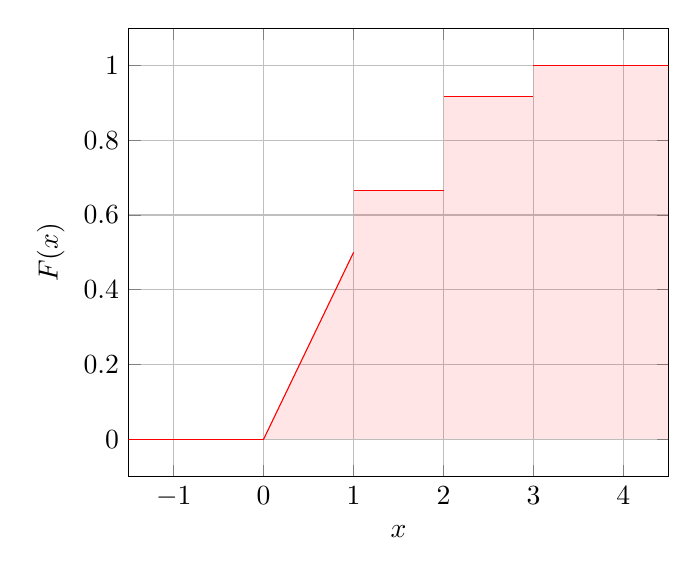
\begin{tikzpicture}
				\begin{axis}[xlabel=$x$, grid = both, ylabel = $F(x)$, xmin = -1.5, xmax = 4.5]
					\addplot[draw=red][name path = f1, domain = -2:0]{0};
					\addplot[draw=red][name path = f2, domain = 0:1]{x/2};
					\addplot[draw=red][name path = f3, domain = 1:2]{2/3};
					\addplot[draw=red][name path = f4, domain = 2:3]{11/12};
					\addplot[draw=red][name path = f5, domain = 3:5]{1};
					
					\path[name path=axis1] (axis cs:-2,0) -- (axis cs:0,0);
					\path[name path=axis2] (axis cs:0,0) -- (axis cs:1,0);
					\path[name path=axis3] (axis cs:1,0) -- (axis cs:2,0);
					\path[name path=axis4] (axis cs:2,0) -- (axis cs:3,0);
					\path[name path=axis5] (axis cs:3,0) -- (axis cs:5,0);
					
					\addplot [thick,color=red,fill=red, fill opacity=0.1] fill between[of=f1 and axis1,];
					\addplot [thick,color=red,fill=red, fill opacity=0.1] fill between[of=f2 and axis2,];
					\addplot [thick,color=red,fill=red, fill opacity=0.1] fill between[of=f3 and axis3,];
					\addplot [thick,color=red,fill=red, fill opacity=0.1] fill between[of=f4 and axis4,];
					\addplot [thick,color=red,fill=red, fill opacity=0.1] fill between[of=f5 and axis5,];
				\end{axis}
			\end{tikzpicture}
		\end{figure}
		
		\item $ P \left\{X > 1/2\right\} = 1 - F(1/2) $, from the plot above, this is $ 3/4 $ \\
		
		\item $ P \left\{ 2 < X \leq 4 \right\} = F(4) - F(2) = 1/12 $ \\
		
		\item $ P \left\{ X < 3 \right\} = F(4) - F(2) = 11/12 $ when asymptotically approaching $ x = 3 $ from the left.
		
		\item  \begin{align}
			P \left\{ X = 1 \right\} = F(1) - \lim\limits_{x \to 1^-} F(x) = \frac{2}{3} - \frac{1}{2} = \frac{1}{6} \nonumber
		\end{align}
		
	\end{enumerate}
	
	\item 
	
		\begin{enumerate}
			\item \begin{align}
				\int\limits_{-\infty}^{\infty} f(x)\ \mathrm{d}x &= 1 \nonumber \\
				%
				\int\limits_{0}^{1} c x^3\ \mathrm{d}x &= 1 \nonumber\\
				%
				\frac{c}{4}\ (x^4) \Big|_0^1 &= 1 \qquad \to \qquad c = 4
			\end{align}
			
			\item \begin{align}
				P \left\{0.4 < X < 0.8 \right\} = \int\limits_{0.4}^{0.8} 4 x^3\ \mathrm{d}x = 0.384
			\end{align}
		\end{enumerate}
	
	
	\item normalization constraint demands \\
	
		\begin{align}
			\int\limits_{-\infty}^{\infty} f(x)\ \mathrm{d}x &= 1 \nonumber \\
			%
			\int\limits_{0}^{\infty} \lambda \exp(-0.01x)\ \mathrm{d}x &= 1 \nonumber\\
			%
			-100 \lambda \ \exp(-0.01x) \Big|_0^\infty &= 1 \qquad \to \qquad \lambda = \frac{1}{100} \\
			%
			P \left\{50 < X < 150 \right\} &= \int\limits_{50}^{150}\ 0.01\ \exp(-0.01x)\ \mathrm{d}x \nonumber \\
			%
			&= \exp(-0.01x)\ \Big|_{150}^{50} = 0.3834 \\
			%\int\limits_{0}^{\infty} \lambda \exp(-0.01x)\ \mathrm{d}x &= 1 \nonumber\\
			%
			P \left\{X < 100 \right\} &= \int\limits_{0}^{100}\ 0.01\ \exp(-0.01x)\ \mathrm{d}x \nonumber \\
			%
			&= \exp(-0.01x)\ \Big|_{100}^{0} = 0.6321
		\end{align}
	
	
	\item Let E be the event that a radio set fails within 150 hours. $ E = \left\{ X < 150 \right\} $ \\
	
		\begin{align}
			P(E) &= \int\limits_{-\infty}^{150} f(x) \ \mathrm{d}x \nonumber\\
			%
			&= \int\limits_{100}^{150} \frac{100}{x^2} \ \mathrm{d}x \nonumber\\
			%
			&= \frac{100}{x}\ \Big|_{150}^{100} = \frac{1}{3} \\
			%
			P(\text{exactly 3 fail}) &= \Mycomb[5]{2} \ (P(E))^2 (1 - P(E))^3 = \frac{10 \times 8}{243} = 0.33
		\end{align}
	
	
	\item normalization constraint demands \\
	
		\begin{align}
			\int\limits_{-\infty}^{\infty} f(x)\ \mathrm{d}x &= 1 \nonumber \\
			%
			\int\limits_{0}^{\infty} c \ \exp(-2x)\ \mathrm{d}x &= 1 \nonumber\\
			%
			-\frac{c}{2} \ \exp(-2x) \Big|_0^\infty &= 1 \qquad \to \qquad c = 2 \\
			%
			P \left\{X > 2 \right\} &= \int\limits_{2}^{\infty}\ 2\ \exp(-2x)\ \mathrm{d}x \nonumber \\
			%
			&= \exp(-2x)\ \Big|_{\infty}^{2} = 0.0183
		\end{align}
	
	
	\item joint PMF of $ N_1, N_2 $, given 3 out of 5 are defective. $ N_1 \in \left\{1, 2, 3\right\} $ and $ N_2 \in \left\{ 1, 2, 3 \right\} $. Using the notation $ P(N_1, N_2) $\\
	
	\begin{align}
		P(1, 1) = \frac{\Mycomb[3]{1}}{\Mycomb[5]{3}} = \frac{3}{10} \nonumber \\
		%
		P(1, 2) = \frac{\Mycomb[2]{1}}{\Mycomb[5]{3}} = \frac{2}{10} \nonumber \\
		%
		P(1, 3) = \frac{\Mycomb[1]{1}}{\Mycomb[5]{3}} = \frac{1}{10} \nonumber \\
		%
		P(2, 1) = \frac{\Mycomb[2]{1}}{\Mycomb[5]{3}} = \frac{2}{10} \nonumber \\
		%
		P(2, 2) = \frac{\Mycomb[1]{1}}{\Mycomb[5]{3}} = \frac{1}{10} \nonumber \\
		%
		P(3, 1) = \frac{\Mycomb[1]{1}}{\Mycomb[5]{3}} = \frac{1}{10} \nonumber \\
	\end{align}
	
	\item 
	\begin{enumerate}
		
			\item 
			normalization constraint demands \\
			\begin{align}
				\int\limits_{0}^{2} \int\limits_{0}^{1} f(x, y)\ \mathrm{d}x \ \mathrm{d}y &= P(S) \nonumber \\
				%
				\int\limits_{0}^{2} \int\limits_{0}^{1} \frac{6x^2}{7} + \frac{3xy}{7}\ \mathrm{d}x \ \mathrm{d}y &= P(S) \nonumber\\
				%
				\int\limits_{0}^{2} \left(\frac{2x^3}{7} \Big|_0^1 + y \times \frac{3x^2}{14} \Big|_0^1  \right) \ \mathrm{d}y &= P(S) \nonumber \\
				%
				\int\limits_{0}^{2} \frac{3y + 4}{14}\ \mathrm{d}y &= P(S) \nonumber \\
				%
				\frac{3y^2 + 8y}{28} \Big|_0^2 &= P(S) = 1
			\end{align}
			
			\item to find the marginal PDF of $ X $,
			\begin{align}
				f_X (x) &= \int\limits_{0}^{2} f(x, y)\ \mathrm{d}y \nonumber \\
				%
				&= \left( \frac{6x^2}{7} \times y \Big|_0^2 + \frac{3x}{14} \times y^2 \Big|_0^2  \right) \nonumber \\
				%
				&= \frac{12x^2 + 6x}{7}
			\end{align}
			
			\item to find $ P \left\{ X > Y \right\} $\\
			
			\begin{align}
				P\left\{ X > Y\right\} &= \int\limits_{0}^{1} \int\limits_{y}^{1} f(x, y)\ \mathrm{d}x \ \mathrm{d}y \nonumber \\
				%
				&= \int\limits_{0}^{1} \left(\frac{2x^3}{7} \Big|_y^1 + y \times \frac{3x^2}{14} \Big|_y^1  \right) \ \mathrm{d}y  \nonumber \\
				%
				&= \int\limits_{0}^{1} \frac{4 - 4y^3 + 3y - 3y^3}{14} \ \mathrm{d}y  \nonumber \\
				%
				&= \frac{1}{14} \left( 4y + \frac{3y^2}{2} - \frac{7y^4}{4} \right)\Big|_0^1 \ \mathrm{d}y  = \frac{15}{56}
			\end{align}
			
		
	\end{enumerate}
	
	\item to find the CDF, find the probability that none of the RVs are larger than $ M $. Given the RVs are independent,
	
	
		\begin{align}
			P\left\{X_i \leq x \right\} &= \frac{x}{1} = x \nonumber \\
			%
			F_M (x) &= P\left\{M \leq x\right\} = P\left\{X_1 \leq x, \dots , X_n \leq x\right\} \nonumber \\
			%
			F_M (x) &= \prod_{i = 1}^{n} x = x^n \qquad \text{for} \qquad x \in \left[0, 1\right] \\
			%
			f_M (x) & = \frac{\mathrm{d}}{\mathrm{d} x} F(x) = nx^{n-1} \qquad x \in \left[0, 1\right]
		\end{align}
	
	
	\item 
		\begin{enumerate}
			\item To compute the marginal PDF of $ X $, 
			\begin{align}
				f_X (x) &= \int\limits_{0}^{\infty} f(x, y)\ \mathrm{d}y \nonumber \\
				%
				&= x e^{-x} \int\limits_{0}^{\infty} e^{-y}\ \mathrm{d}y \nonumber \\
				%
				&= x e^{-x} \left(e^{-y}\Big|_\infty^0\right) = x e^{-x}
			\end{align}
			
			\item To compute the marginal PDF of $ y $, 
			\begin{align}
				f_Y (y) &= \int\limits_{0}^{\infty} f(x, y)\ \mathrm{d}x \nonumber \\
				%
				&= e^{-y} \int\limits_{0}^{\infty} x\ e^{-x}\ \mathrm{d}x \nonumber \\
				%
				&= e^{-y} \left(xe^{-x}\Big|_\infty^0 + \int\limits_{0}^{\infty} e^{-x} \ \mathrm{d}x\right) = e^{-y}
			\end{align}
			
			\item $ f_X (x) \times f_Y (y)  = x e^{-(x + y)}$, which is equal to the joint PDF. Hence, $ X, Y $ are independent.
		\end{enumerate}
	
	
	\item 
		\begin{enumerate}
			\item To compute the marginal PDF of $ X $, 
			\begin{align}
				f_X (x) &= \int\limits_{0}^{\infty} f(x, y)\ \mathrm{d}y \nonumber \\
				%
				&= x e^{-x} \int\limits_{0}^{\infty} e^{-y}\ \mathrm{d}y \nonumber \\
				%
				&= x e^{-x} \left(e^{-y}\Big|_\infty^0\right) = x e^{-x}
			\end{align}
			
			\item To compute the marginal PDF of $ y $, 
			\begin{align}
				f_Y (y) &= \int\limits_{0}^{y} f(x, y)\ \mathrm{d}x \nonumber \\
				%
				&= \int\limits_{0}^{y} 2\ \mathrm{d}x = 2y  \qquad y \in (0, 1) \\
				%
				f_X (x) &= \int\limits_{x}^{1} f(x, y)\ \mathrm{d}y \nonumber \\
				%
				&= \int\limits_{x}^{1} 2\ \mathrm{d}y  = 2(1 - x)  \qquad x \in (0, 1)
			\end{align}
			
			\item $ f_X (x) \times f_Y (y)  = 4y(1-x)$, which is not equal to the joint PDF. Hence, $ X, Y $ are not independent.
		\end{enumerate}
	
	
	\item  
		To compute the marginal PDF of $ X $ and $ Y $ separately, 
		\begin{align}
			f_X (x) &= \int\limits_{-\infty}^{\infty} f(x, y)\ \mathrm{d}y \nonumber \\
			%
			&= k(x) \int\limits_{-\infty}^{\infty} h(y)\ \mathrm{d}y \\
			%
			f_Y (y) &= \int\limits_{-\infty}^{\infty} f(x, y)\ \mathrm{d}x \nonumber \\
			%
			&= h(y) \int\limits_{-\infty}^{\infty} k(x)\ \mathrm{d}x
		\end{align}
		
		To check whether $ X, Y $ are independent,
		\begin{align}
			f_X (x) \times f_Y (y) &= h(y) \ k(x) \ \int\limits_{-\infty}^{\infty} k(x)\ \mathrm{d}x \ \int\limits_{-\infty}^{\infty} h(y)\ \mathrm{d}y \nonumber \\
			%
			&= h(y) \ k(x)\ \int\limits_{-\infty}^{\infty} \int\limits_{-\infty}^{\infty} h(y) k(x) \ \mathrm{d}x \ \mathrm{d}y  \nonumber \\
			%
			&= k(x)\ h(y) = f(x, y)
		\end{align}
		Hence, $ X, Y $ are independent. In the relation above, the integral of $ f(x, y) $ over the full domains of $ X, Y $ was 1 from the normalization condition.
	
	
	\item The previous problems do obey the factoring rule.
	
	\item 
		\begin{enumerate}
			\item \begin{align}
				P \left\{X + Y \leq a \right\} &= P \left\{ X \leq a - Y \right\} \nonumber \\
				%
				&= \int\limits_{-\infty}^{\infty} \int\limits_{-\infty}^{a - y} f_Y (y) \ f_X(x) \ \mathrm{d}x \ \mathrm{d}y  \nonumber \\
				%
				&= \int\limits_{-\infty}^{\infty} f_Y (y) \ F_X(a - y) \ \mathrm{d}y 
			\end{align}
			
			\item \begin{align}
				P \left\{ X \leq Y \right\} &= \int\limits_{-\infty}^{\infty} \int\limits_{-\infty}^{y} f_Y (y) \ f_X(x) \ \mathrm{d}x \ \mathrm{d}y  \nonumber \\
				%
				&= \int\limits_{-\infty}^{\infty} f_Y (y) \ F_X(y) \ \mathrm{d}y 
			\end{align}
		\end{enumerate}
	
	
	\item To find the PDF, first find the CDF and then differentiate it. Note that the integral over current is split into two parts, one with constraint on resistance and other without.
	
		\begin{align}
			P \left\{ W \leq a \right\} &= F_W (a) \nonumber \\
			%
			&= \int\limits_{0}^{\sqrt{a}} \int\limits_{0}^{1}  f_R (y) \ f_I(x) \ \mathrm{d}x \ \mathrm{d}y  + \int\limits_{\sqrt{a}}^{1} \int\limits_{0}^{a/x^2}  f_R (y) \ f_I(x) \ \mathrm{d}x \ \mathrm{d}y \nonumber \\
			%
			&= \int\limits_{0}^{\sqrt{a}}  6x(1-x) \ \mathrm{d}x + \int\limits_{\sqrt{a}}^{1} \frac{a^2\ 6x(1-x)}{x^4} \ \mathrm{d}x \nonumber \\
			%
			&= \left(3x^2 - 2x^3\right) \Big|_0^{\sqrt{a}} + 6a^2\ \left(\frac{-2}{x^2} + \frac{1}{x}\right)\Big|_{\sqrt{a}}^{1} \nonumber \\
			%
			&= 3a - 2a^{3/2} - 6a^2 + 12a -6a^{3/2} \nonumber \\
			%
			&= - 6a^2 - 8a^{3/2} + 15a \\
			%
			f_W (a) &= \frac{\mathrm{d}}{\mathrm{d} a} F_W (a) = -12a - 12a^{1/2} + 15
		\end{align}
	
	
	\item to determine $ P \left\{B\ |\ G = 2\right\} $. Also, define $ T = G+B $ \\
	
		\begin{align}
			P \left\{G = 2\right\} &= P \left\{G = 2\ |\ T = 0\right\}P \left\{T = 0\right\} \nonumber \\
			%
			&+ P \left\{G = 2\ |\ T = 1\right\}P \left\{T = 1\right\} \nonumber \\ 
			%
			&+ P \left\{G = 2\ |\ T = 2\right\}P \left\{T = 2\right\} \nonumber \\
			%
			&+ P \left\{G = 2\ |\ T = 3\right\}P \left\{T = 3\right\} \nonumber \\
			%
			&= 0 \times 0.15 + 0 \times 0.2 + \frac{1}{4} \times 0.35 + \frac{1}{8} \times 0.3 \nonumber \\
			%
			&= \frac{1}{8} \\
			%
			P \left\{B = 0\ |\ G = 2\right\} &= \frac{P \left\{B = 0, G = 2\right\}}{P \left\{G = 2\right\}} = \frac{1/4 \times 0.35}{1/8} = \frac{7}{10} \\
			%
			P \left\{B = 1\ |\ G = 2\right\} &= \frac{P \left\{B = 1, G = 2\right\}}{P \left\{G = 2\right\}} = \frac{1/8 \times 0.3}{1/8} = \frac{3}{10}
		\end{align}
	
	
	\item to find the conditional PDF,
	
		\begin{enumerate}
			\item From problem 10 \\
			\begin{align}
				f_{X|Y}(x\ |\ y) &= P \left\{ X = x\ |\ Y = y \right\} = \frac{f(x, y)}{f_Y(y)}\nonumber\\
				%			
				f_Y (y) &= \int\limits_{0}^{1} f(x, y)\ \mathrm{d}x \nonumber \\
				%
				&= \left( \frac{2x^3}{7} \Big|_0^1 + 3y \times \frac{x^2}{14}\Big|_0^1  \right) \nonumber \\
				%
				&= \frac{4 + 3y}{14} \\
				%
				f_{X|Y}(x\ |\ y) &= \frac{12x^2 + 6xy}{3y + 4} \qquad x \in \left(0, 1\right)
			\end{align}
			
			\item From problem 13 \\
			\begin{align}
				f_{X|Y}(x\ |\ y) &= P \left\{ X = x\ |\ Y = y \right\} = \frac{f(x, y)}{f_Y(y)}\nonumber\\
				%			
				f_{X|Y}(x\ |\ y) &= \frac{2}{2(1-x)} = \frac{1}{1-x} \qquad x \in \left(0, 1\right)
			\end{align}
		\end{enumerate}
	
	
	\item 
	
		\begin{enumerate}
			\item Assuming $ f_Y (y) $ is well defined in the domain of interest,
			\begin{align}
				f_{X|Y}(x\ |\ y) &= P \left\{ X = x\ |\ Y = y \right\} = \frac{f(x, y)}{f_Y(y)} \nonumber\\
				%
				f(x,y) &= f_X (x) \times f_Y (y) \quad \leftrightarrow \quad \text{X, Y are independent}  \nonumber\\
				%
				f_{X|Y}(x\ |\ y) &= f_X (x) \quad \leftrightarrow \quad \text{X, Y are independent}
			\end{align}
			
			\item Exactly same steps as the above
		\end{enumerate}
	
	
	\item Using data from Problem 1,
	\begin{align}
		\mathbb{E}[X] &= \sum\limits_{i} x_i\ P \left\{ X = x_i \right\} \nonumber \\
		%
		&= 1 \times \frac{1}{2} + 2 \times \frac{25}{90} + 3 \times \frac{100}{720} + 4 \times \frac{15}{252} + 5 \times \frac{5}{252} + 6 \times \frac{1}{252} \nonumber \\
		%
		&= 1.8333
	\end{align}
	
	\item Using data from Problem 3,
	\begin{align}
		\mathbb{E}[X] &= \sum\limits_{i} x_i\ P \left\{ X = x_i \right\} \nonumber \\
		%
		&= (-1) \times \frac{3}{8} + 1 \times \frac{3}{8} + (-3) \times \frac{1}{8} + 3 \times \frac{1}{8} \nonumber \\
		%
		&= 0 \qquad \text{intuitive from the symmetry}
	\end{align}
	
	\item Let the score be random variable $ X $ and the actual belief probability be $ a $,
	
		\begin{align}
			\mathbb{E}[X] &= \sum\limits_{i} x_i\ P \left\{ X = x_i \right\} \nonumber \\
			%
			&= (2p - p^2)	 \times a +  (1 - p^2) \times (1-a) \nonumber \\
			%
			&= -p^2 + 2ap + (1-a) \nonumber \\
			%
			\mathbb{E}'[X] &= \frac{\mathrm{d}}{\mathrm{d} p} \mathbb{E}[X] = -2p + 2a \\
			%
			p &= a \quad \text{setting} \quad 	\mathbb{E}'[X] = 0
		\end{align}
	
	
	\item Let the profit be $ X $ and the policy cost be $ Y $\\
	
	
		\begin{align}
			\mathbb{E}[X] &= \sum\limits_{i} x_i\ P \left\{ X = x_i \right\} \nonumber \\
			%
			&= (Y - A) \times p + (Y - 0)(1-p) = 0.1\ A\\
			%
			Y &= (p + 0.1)\ A 
		\end{align}
	
	
	\item Let the buses be $ A, B, C, D $ and the student, driver RVs be $ X, Y $.
	
		\begin{enumerate}
			
			\item The more populated buses are more likely to be selected when randomly picking a student, but not when randomly picking a driver. So, $ \mathbb{E}[X] > \mathbb{E}[Y] $ \\
			
			
			\item \begin{align}
				\mathbb{E}[X] &= \sum\limits_{i} x_i\ P \left\{ X = x_i \right\} \nonumber \\
				%
				&= 40 \times \frac{40}{148} + 33 \times \frac{33}{148} + 25 \times \frac{25}{148} + 50 \times \frac{50}{148}\\
				%
				&= 39.28
			\end{align}
			
			\item \begin{align}
				\mathbb{E}[Y] &= \sum\limits_{i} y_i\ P \left\{ Y = y_i \right\} \nonumber \\
				%
				&= 40 \times \frac{1}{4} + 33 \times \frac{1}{4} + 25 \times \frac{1}{4} + 50 \times \frac{1}{4}\\
				%
				&= 37
			\end{align}
			
		\end{enumerate}
	
	
	\item Finding the PMF of the random variable $ X $ which is the number of games played for the series to end, $ X \in \left\{i, 2i-1\right\} $\\
	
	
		\begin{align}
			P \left\{X = 2\right\} &= p^2 + (1-p)^2 \nonumber \\
			%
			P \left\{X = 3\right\} &= p^2 (1-p) + (1-p)^2 p \nonumber \\
			%
			\mathbb{E}[X] &= 2 \times P \left\{X = 2\right\} + 3 \times P \left\{X = 3\right\} \\
			%
			&= 4p^2 + 2 - 4p + 3p^2 + 3p - 6p^2 \nonumber \\
			%
			&= p^2 - p + 2 \nonumber \\
			%
			\mathbb{E}'[X] &= \frac{\mathrm{d}}{\mathrm{d} p} \mathbb{E}[X] = 2p - 1 \\
			%
			p &= 1/2 \quad \text{setting} \quad 	\mathbb{E}'[X] = 0			
		\end{align}
	
	
	\item 
		\begin{align}
			\mathbb{E}[X] &= \int\limits_{0}^{1} x\ f(x)\ \mathrm{d}x \nonumber \\
			%
			&= \left( \frac{ax^2}{2} \Big|_0^1 + \frac{bx^4}{4}\Big|_0^1  \right) = \frac{3}{5} \nonumber \\
			% 
			2a + b &= 12/5 \\
			%
			\text{normalization constraint} &\to  \int\limits_{0}^{1}  f(x)\ \mathrm{d}x = 1 \nonumber \\
			%
			&= \left( ax \Big|_0^1 + \frac{bx^3}{3}\Big|_0^1  \right) = 1 \nonumber \\
			% 
			3a + b &= 3 \\
			%
			a &= \frac{3}{5} \quad \text{and} \quad b = \frac{6}{5} 
		\end{align}
	
	
	\item Using integration by parts twice,
	
		\begin{align}
			\mathbb{E}[X] &= \int\limits_{0}^{\infty} x\ f(x)\ \mathrm{d}x \nonumber \\
			%
			&= \int\limits_{0}^{\infty} a^2 x^2\ \exp(-ax)\ \mathrm{d}x \nonumber \\
			% 
			&= -a x^2\ \exp(-ax) + \int\limits_{0}^{\infty} 2a x\ \exp(-ax)\ \mathrm{d}x \nonumber \\
			%
			&= -a x^2\ \exp(-ax) - 2x\ \exp(-ax)  + \int\limits_{0}^{\infty} 2\ \exp(-ax)\ \mathrm{d}x \nonumber \\
			%
			&= -a x^2\ \exp(-ax) - 2x\ \exp(-ax)  -  2/a \ \exp(-ax)  \Big|_0^\infty \nonumber \\
			%
			&= 2/a 
		\end{align}
	
	
	\item RVs are independent with same PDF,
	
		\begin{enumerate}
			\item Finding the CDF of the maximum $ Y $, and then its PDF\\
			\begin{align}
				F_Y (y) &= P\left\{X_1 < y, X_2 < y \dots X_n < y\right\} \nonumber \\
				%
				&= y^n \\
				%
				f_Y (y) &= \frac{\mathrm{d}}{\mathrm{d} y} F_Y (y) = n\ y^{n-1} \\
				%
				\mathbb{E}[Y] &= \int\limits_{0}^{1} y\ f(y)\ \mathrm{d}y = \frac{n}{n+1} \\
			\end{align}
			
			\item Finding the CDF of the minimum $ Z $, and then its PDF\\
			\begin{align}
				F_Z (z) &= P\left\{X_1 > z, X_2 > z \dots X_n > z\right\} \nonumber \\
				%
				&= (1-z)^n \\
				%
				f_Z (z) &= \frac{\mathrm{d}}{\mathrm{d} z} F_Z (z) = n\ (1 - z)^{n-1} \\
				%
				\mathbb{E}[Z] &= \int\limits_{0}^{1} z\ f(z)\ \mathrm{d}z \nonumber \\
				%
				&= \int\limits_{0}^{1} nz\ (1 - z)^{n-1}\ \mathrm{d}z = \int\limits_{0}^{1} n(1 - u)\ (u)^{n-1}\ \mathrm{d}u \nonumber \\
				%
				&= \left(u^n\ - \frac{n u^{n+1}}{n+1}\right)  \Big|_0^1 = \frac{1}{n+1}
			\end{align}
			
		\end{enumerate}
	
	
	\item Two alternate approaches used assuming $ n \geq 1 $,
	
		\begin{enumerate}
			
			\item Finding the PDF for $ Y = X^n $ and then the expected value,
			
			\begin{align}
				F_Y (y) &= P \left\{x^n \leq y\right\} = P \left\{x \leq y^{1/n}\right\} = y^{1/n} \\
				%
				f_Y (y)&= \frac{\mathrm{d}}{\mathrm{d} y} F_Y (y) = \frac{y^{1/n}}{ny} \\
				%
				\mathbb{E}[Y] &= \int\limits_{0}^{1} y\ f_Y (y)\ \mathrm{d}y = \frac{y^{1 + 1/n}}{n + 1} \Big|_0^1 = \frac{1}{n+1}
			\end{align}
			\item Finding the expected value directly,
			\begin{align}
				\mathbb{E}[X^n] &= \int\limits_{0}^{1} x^n\ f(x)\ \mathrm{d}x = \frac{x^{n+1}}{n+1} \Big|_0^1 = \frac{1}{n+1}
			\end{align}
			
		\end{enumerate}
	
	
	\item Let $ C(x) = 40 + 30 \sqrt{x} $
	
		\begin{align}
			\mathbb{E}[C(x)] &= \int\limits_{0}^{2} C(x)\ f(x)\ \mathrm{d}x \nonumber \\
			%
			&= \int\limits_{0}^{2} 20 + 15 \sqrt{x}\ \mathrm{d}x \nonumber \\
			%
			&= 20x + 10 x^{3/2} \ \Big|_0^2 \nonumber \\
			%
			&= 20\sqrt{2} + 40 = 68.28
		\end{align}
	
	
	\item $ \mathbb{E}[X] = 2 $, $ \mathbb{E}[X^2] = 8 $ \\
	
		\begin{enumerate}
			
			\item \begin{align}
				\mathbb{E}[(2 + 4X)^2] &= \mathbb{E}[4 + 16X + 16X^2] \nonumber \\
				%
				&= \mathbb{E}[4] + 16\mathbb{E}[X] + 16 \mathbb{E}[X^2] \nonumber \\
				%
				&= 164
			\end{align}
			
			\item \begin{align}
				\mathbb{E}[X^2 + (X + 1)^2] &= \mathbb{E}[1 + 2X + 2X^2] \nonumber \\
				%
				&= \mathbb{E}[1] + 2 \mathbb{E}[X] + 2 \mathbb{E}[X^2] \nonumber \\
				%
				&= 21
			\end{align}
			
		\end{enumerate}
	
	
	\item 17 white and 23 black balls, with $ X $ measuring number of white balls chosen out of a total 10.
	
		\begin{enumerate}
			
			\item Indicator variables looking at whether a chosen ball is white
			\begin{align}
				\mathbb{E}[X] &= \sum\limits_{i = 1}^{10} \mathbb{E}[X_i] \nonumber \\
				%
				&= 10\ \mathbb{E}[X_1] \nonumber \\
				%
				&= 10\ \sum\limits_{k = 1}^{10} P \left\{ X_1 = 1\ |\ X = k \right\} \ P\left\{X = k\right\} \nonumber \\
				%
				&= 10\ \sum\limits_{k = 1}^{10} \frac{k}{10} \ \frac{\Mycomb[17]{k}\ \Mycomb[23]{10-k}}{\Mycomb[40]{10}} \nonumber \\
				%
				&= 4.25
			\end{align}
			
			\item Indicator variables looking at whether a white ball is chosen
			\begin{align}
				\mathbb{E}[X] &= \sum\limits_{i = 1}^{17} \mathbb{E}[Y_i] \nonumber \\
				%
				&= 17\ \mathbb{E}[Y_1] \nonumber \\
				%
				&= 17\ \sum\limits_{k = 1}^{10} P \left\{ Y_1 = 1\ |\ X = k \right\} \ P\left\{X = k\right\} \nonumber \\
				%
				&= 17\ \sum\limits_{k = 1}^{10} \frac{k}{17} \ \frac{\Mycomb[17]{k}\ \Mycomb[23]{10-k}}{\Mycomb[40]{10}} \nonumber \\
				%
				&= 4.25
			\end{align}
			
		\end{enumerate}
	
	
	\item Using the PDF, find the parameter value which gives a CDF value of $ 1/2 $.
	
		\begin{enumerate}
			
			\item 	\begin{align}
				F(a) &= \int\limits_{0}^{a} f(x)\ \mathrm{d}x \nonumber \\
				%
				&= \int\limits_{0}^{a} e^{-x}\ \mathrm{d}x \nonumber \\
				%
				&= 1 - e^{-a} \nonumber \\
				%
				F(m) &= 0.5 = 1 - e^{-m} \nonumber \\
				%
				m &= \ln (2)
			\end{align}
			
			\item 	\begin{align}
				F(a) &= \int\limits_{0}^{a} f(x)\ \mathrm{d}x \nonumber \\
				%
				&= \int\limits_{0}^{a} 1\ \mathrm{d}x \nonumber \\
				%
				&= a \nonumber \\
				%
				F(m) &= 0.5 = 1 - a \nonumber \\
				%
				m &= 0.5
			\end{align}
			
		\end{enumerate}
	
	
	
	\item Using the CDF and PDF given, find the value minimizing $ \mathbb{E}[\left|X - c\right|] $, by setting its derivative to zero.
	
		\begin{align}
			\mathbb{E}[\left|X - c\right|] &= \int\limits_{-\infty}^{c} (c - x)\ f(x)\ \mathrm{d}x + \int\limits_{c}^{\infty} (x - c)\ f(x)\ \mathrm{d}x \nonumber \\
			%
			&= \int\limits_{-\infty}^{c} (c - x)\ f(x)\ \mathrm{d}x + \int\limits_{c}^{\infty} (x - c)\ f(x)\ \mathrm{d}x \nonumber \\
			%
			&= c\ F(c) - \int\limits_{-\infty}^{c} x\ f(x)\ \mathrm{d}x + \int\limits_{c}^{\infty} x\ f(x)\ \mathrm{d}x - c\ (1 - F(c)) \nonumber \\
			%
			\frac{\mathrm{d}}{\mathrm{d} c} \mathbb{E}[\left|X - c\right|] &= -1 + 2F(c) + 2c\  \frac{\mathrm{d}}{\mathrm{d} c}\ F(c) - c\ f(c) \times 1 - c\ f(c) \times 1 \nonumber \\
			%
			&= -1 + 2F(c) \nonumber \\
			%
			\text{minimizing}\ &\to\ F(c) = 0.5
		\end{align}
	
	
	\item Defining the percentile as $ F(m_p) = p $.
	
		\begin{align}
			F(m_p) &= \int\limits_{0}^{m_p} f(x)\ \mathrm{d}x \nonumber \\
			%
			&= \int\limits_{0}^{m_p} 2\ \exp(-2x)\ \mathrm{d}x \nonumber \\
			%
			&= -\exp(-2x)\ \Big|_{0}^{m_p} \\
			%
			p &= 1 - \exp(-2\ m_p) \nonumber \\
			%
			m_p &= - \frac{\ln(1 - p)}{2}
		\end{align}
	
	
	\item Using the indicator variable for a couple remaining intact $ X_i $, only if both members survive,
	
		\begin{align}
			\mathbb{E}[X] &= \sum\limits_{i = 1}^{100} \mathbb{E}[X_i] \nonumber \\
			%
			&= 100\ \mathbb{E}[X_1] \nonumber \\
			%
			&= 100\ \frac{\Mycomb[198]{50}}{\Mycomb[200]{50}} \nonumber \\
			%
			&= 56.15
		\end{align}
	
	
	\item $ n $ independent trials, each success with probability $ p $, with indicator variables $ X_i $ \\
	
		\begin{align}
			\mathbb{E}[X] &= \sum\limits_{i = 1}^{n} \mathbb{E}[X_i] \qquad \text{independence not required} \nonumber \\
			%
			&= n\ \mathbb{E}[X_1] \nonumber \\
			%
			&= np   \\
			%
			\mathrm{Var}(X_i) &= \mathbb{E}[X_i]\ (1 - \mathbb{E}[X_i]) \nonumber \\
			%
			&= p\ (1 - p) \nonumber \\
			%
			\mathrm{Var}(X) &= \sum\limits_{i = 1}^{n} \mathrm{Var}(X_i) \qquad \text{only if independent} \nonumber \\
			%
			&= np\ (1-p)
		\end{align}
	
	
	\item $X = \left\{1, 2, 3, 4\right\} $ equally probable.
	
		\begin{enumerate}
			
			\item 	\begin{align}
				\mathbb{E}[X] &= \sum\limits_{i = 1}^{4} \mathbb{E}[X_i] \nonumber \\
				%
				&= \frac{1}{4} \times 1 + \frac{1}{4} \times 2 + \frac{1}{4} \times 3 + \frac{1}{4} \times 4 \nonumber \\
				%
				&= 2.5   \\
			\end{align}
			
			\item 	\begin{align}
				\mathbb{E}[X^2] &= \frac{1}{4} \times 1^2 + \frac{1}{4} \times 2^2 + \frac{1}{4} \times 3^2 + \frac{1}{4} \times 4^2 \nonumber \\
				%
				&= 7.5 \\
				%
				\mathrm{Var}(X) &= \mathbb{E}[X^2] - (\mathbb{E}[X])^2 \nonumber \\
				%
				&= 7.5 - 2.5^2 = 1.25
			\end{align}
			
		\end{enumerate}
	
	
	
	\item $\mathbb{E}[X] = 2 $. Three possible events with probabilities $ p_1, p_2, p_3 $, with $ p_1 + p_2 + p_3  = 1$\\
	
		\begin{enumerate}
			
			\item 	\begin{align}
				\mathbb{E}[X] &= \sum\limits_{i = 1}^{3} i\ P\left\{X = i\right\} \nonumber \\
				%
				&= p_1 + 2p_2 + 3p_3 \nonumber \\
				%
				&= 2   \\
				%
				\mathbb{E}[X^2] &= 1^2 \times p_1 + 2^2 \times p_2 + 3^2 \times p_3 \nonumber \\
				%
				&= p_1 + 4 p_2 + 9 p_3 \nonumber \\
			\end{align}
			
			\item Extremizing the variance involves first substituting $ p_2, p_3 $ in favour of $ p_1 $,
			\begin{align}
				\mathrm{Var}(X) &= \mathbb{E}[X^2] - (\mathbb{E}[X])^2 \nonumber \\
				%
				&= p_1 + 4 p_2 + 9 p_3 - 4 \nonumber \\
				%
				p_3 &= 1 - p_1 - p_2 \nonumber \\
				%
				2 &= 3 -2p_1 - p_2 \nonumber \\
				%
				p_2 &= 1 - 2p_1 \qquad \text{and} \qquad p_3 = p_1 \\
				%
				\mathrm{Var}(X) &= 2p_1
			\end{align}
			
			maximizing $ \mathrm{Var}(X) $, involves maximizing $ p_1 $ and vice versa,
			maximum variance is 1, minimum is 0.
			
		\end{enumerate}
	
	
	\item $ 3 $ independent trials, each success with probability $ p = 0.5 $, with indicator variables $ X_i $ for number of heads \\
	
		\begin{align}
			\mathbb{E}[X] &= \sum\limits_{i = 1}^{3} \mathbb{E}[X_i] \qquad \text{independence not required} \nonumber \\
			%
			&= 3\ \mathbb{E}[X_1] \nonumber \\
			%
			&= 1.5   \\
			%
			\mathrm{Var}(X_i) &= \mathbb{E}[X_i]\ (1 - \mathbb{E}[X_i]) \nonumber \\
			%
			&= p\ (1 - p) = 1/4 \nonumber \\
			%
			\mathrm{Var}(X) &= \sum\limits_{i = 1}^{3} \mathrm{Var}(X_i) \qquad \text{only if independent} \nonumber \\
			%
			&= 3/4
		\end{align}
	
	
	\item placeholder solve q 42 \\
	
	\item 
		\begin{enumerate}
			
			\item \begin{align}
				\mathbb{E}[X] &= \int\limits_{8}^{10} x\ f(z)\ \mathrm{d}z \nonumber \\
				%
				&= \int\limits_{8}^{9} (z^2-8z)\ \mathrm{d}z  + \int\limits_{9}^{10} (10z-z^2)\ \mathrm{d}z\nonumber \\
				% 
				&= \left(\frac{z^3}{3} - 4z^2\right) \Big|_8^9  + \left(5z^2 - \frac{z^3}{3}\right) \Big|_9^{10} \\
				%
				&= \frac{13}{3} + \frac{14}{3} = 9 \\
				%
				\mathbb{E}[X^2] &= \int\limits_{8}^{10} z^2\ f(z)\ \mathrm{d}z \nonumber \\
				%
				&= \int\limits_{8}^{9} (z^3-8z^2)\ \mathrm{d}z  + \int\limits_{9}^{10} (10z^2-z^3)\ \mathrm{d}z\nonumber \\
				% 
				&= \left(\frac{z^4}{4} - \frac{8z^3}{3}\right) \Big|_8^9  + \left(\frac{10z^3}{3} - \frac{z^4}{4}\right) \Big|_9^{10} \\
				%
				&= 974/12 \\
				%
				\mathrm{Var}(X) &= \mathbb{E}[X^2]- (\mathbb{E}[X])^2 \nonumber \\
				%
				&= 974/12 - 81 = 1/6 \\
			\end{align}
			
			\item $ C(w) = w/15 + 0.35 $, $ S = 2 $, weight limit $ L = 8.25 $. Let profit be $ Y $\\
			\begin{align}
				P\left\{w \leq L\right\} = F(L) &= \int\limits_{8}^{L} f(w)\ \mathrm{d}w \nonumber \\
				%
				&= \left(\frac{z^2}{2} - 8z\right) \Big|_8^9 \nonumber \\
				%
				&=  1/32\\
				%
				Y(w) &= S - C(w) = 1.65 - w/15  \qquad \text{if } w > L\nonumber \\
				%
				&= - C(w) = -0.35 - w/15  \qquad \text{if } w < L\nonumber \\
				%
				\mathbb{E}[Y(w)] &= \int\limits_{8}^{10} y(w)\ f(w)\ \mathrm{d}w \nonumber \\
				%
				&= \int\limits_{8}^{8.25} (-0.35-w/15)(w-8)\ \mathrm{d}w \nonumber \\
				%
				&+ \int\limits_{8.25}^{9} (1.65 - w/15)(w-8)\ \mathrm{d}w \nonumber \\
				%
				&+ \int\limits_{9}^{10} (1.65-w/15)(10-w)\ \mathrm{d}w \\
				% 
				&= 0.9875 
			\end{align}
		\end{enumerate}
	
	
	\item 
		\begin{enumerate}
			
			\item \begin{align}
				f_X (x) &= \int\limits_{0}^{1-x} f(x, y)\ \mathrm{d}y \nonumber \\
				%
				&= \int\limits_{0}^{1-x} (3x + 3y)\ \mathrm{d}y\nonumber \\
				% 
				&= \left(\frac{3y^2}{2} + 3xy\right) \Big|_0^{1-x} \\
				%
				&= 1.5 (1-x)^2 + 3x - 3x^2 \nonumber \\
				%
				&= 1.5 - 1.5x^2 \\
				%
				f_Y (y) &= 1.5 - 1.5y^2
			\end{align}
			
			\item \begin{align}
				\mathbb{E}[X] &= \int\limits_{0}^{1} x\ f_X (x)\ \mathrm{d}x \nonumber \\
				%
				&= \int\limits_{0}^{1} 1.5x - 1.5x^3\ \mathrm{d}x \nonumber \\
				% 
				&= 0.375 \\
				%
				\mathbb{E}[X^2] &= \int\limits_{0}^{1} x^2\ f_X (x)\ \mathrm{d}x \nonumber \\
				%
				&= \int\limits_{0}^{1} 1.5x^2 - 1.5x^4\ \mathrm{d}x \nonumber \\
				% 
				&= 0.2 \\
				%
				\mathrm{Var}(X) &= \mathbb{E}[X^2]- (\mathbb{E}[X])^2 \nonumber \\
				%
				&= 19/64
			\end{align}
		\end{enumerate}
	
	
	\item 
		\begin{enumerate}
			\item Performing the row sums and column sums gives the marginal probability of $ X_1 $ and $ X_2 $ respectively.
			
			\begin{table}[H]
				\centering
				\begin{tabular}{@{}rr|rr@{}}
					\toprule
					$ X_1 $ & $ p_{X1} $ & $ X_2 $ & $ p_{X2} $ \\ \midrule
					0     & 3/16	& 0	 & - 	 \\
					1     & 2/16    & 1	 & 1/2 	 \\
					2     & 5/16    & 2	 & 1/2 	 \\
					3     & 6/16    & 3	 & - 	 \\ \bottomrule
				\end{tabular}
			\end{table}
			
			\item \begin{align}
				\mathbb{E}[X_1] &= 0 \times 3/16 + 1 \times 2/16 + 2 \times 5/16 + 3 \times 6/16 \nonumber \\
				%
				&= 30/16 \\
				% 
				\mathbb{E}[X_2] &= 3/2 \\
				%
				\mathbb{E}[X_1^2] &= 0 \times 3/16 + 1 \times 2/16 + 4 \times 5/16 + 9 \times 6/16 \nonumber \\
				%
				&= 19/4 \\
				%
				\mathbb{E}[X_2^2] &= 1 \times 1/2 + 4 \times 1/2 \nonumber \\
				%
				&= 5/2 \\
				%
				\mathrm{Var}(X_1) &= 1.234 \\
				%
				\mathrm{Var}(X_2) &= 0.25 \\
				%
				\mathbb{E}[X_1 X_2] &= 0 + 0 + 1/16 + 2/16 + 6/16 + 8/16 + 6/16 + 24/16  \nonumber \\
				%
				&= 47/16 \\
				%
				\mathrm{Cov}(X_1, X_2) &= 1/8 
			\end{align}
		\end{enumerate}
	
	
	\item finding the covariance and then correlation using Problem 44 \\ 
	
		\begin{align}
			\mathbb{E}[XY] &= \int\limits_{0}^{1} \int\limits_{0}^{1-x}  (xy) \ f(x, y) \ \mathrm{d}x \ \mathrm{d}y \nonumber \\
			%
			&= \int\limits_{0}^{1} \int\limits_{0}^{1-x}  3x^2 y + 3x y^2 \ \mathrm{d}x \ \mathrm{d}y \nonumber \\
			%
			&= \int\limits_{0}^{1}  \frac{3x^2}{2} y^2 \Big|_0^{1-x} + x y^3 \Big|_0^{1-x} \ \mathrm{d}x \nonumber \\
			%
			&= \int\limits_{0}^{1}  1.5x^4 + -3x^3 + 1.5x^2 + x - x^4 - 3x^2 + 3x^3  \ \mathrm{d}x \nonumber \\
			%
			&= \int\limits_{0}^{1}  0.5x^4 - 1.5x^2 + x \ \mathrm{d}x \nonumber = 0.1 \\
			%
			\mathrm{Corr}(X, Y) &= \frac{\mathrm{Cov}(X, Y)}{s_x s_y} = \frac{0.1 - 9/64}{19/64} = -\frac{13}{95}
		\end{align}
	
	
	\item 
		\begin{align}
			\mathrm{Cov}(aX, Y) &= \mathbb{E}[aXY] - \mathbb{E}[aX] \ \mathbb{E}[Y] \nonumber \\
			%
			&= a \mathbb{E}[XY] - a\mathbb{E}[X] \ \mathbb{E}[Y] \nonumber \\
			%
			&= a \left(\mathbb{E}[XY] - \mathbb{E}[X] \ \mathbb{E}[Y]\right) \nonumber \\
			%
			&= a \mathrm{Cov}(X, Y)
		\end{align}
	
	
	\item Consider for some $ n $, two random variables $ X_n $ and $ \sum_{1}^{n-1} X_k$. Starting with $ n = 2 $.
	
	\begin{align}
		\mathrm{Cov}\left(\sum\limits_{i = 1}^{2}X_i, Y\right) &= \sum\limits_{i = 1}^{2} \mathrm{Cov}(X_i, Y) 
	\end{align}
	
	By increasing $ n $ iteratively, the proof by induction is straightforward to set up.
	
	\item Once, the two inequalities are proved separately, they combine to prove the $ [-1, 1] $ range for the correlation.
	
		\begin{enumerate}
			
			\item \begin{align}
				\mathrm{Var}\left(\frac{X}{\sigma_x} + \frac{Y}{\sigma_y}\right) &=\mathrm{Var}\left(\frac{X}{\sigma_x}\right) +  \mathrm{Var}\left(\frac{Y}{\sigma_y}\right) + 2\ \mathrm{Cov}\left(\frac{X}{\sigma_x}, \frac{Y}{\sigma_y}\right)  \nonumber \\
				%
				2\ \mathrm{Corr}(X, Y) &\geq - \mathrm{Var}\left(\frac{Y}{\sigma_y}\right) - \mathrm{Var}\left(\frac{X}{\sigma_x}\right) \\
				%
				&\geq - \frac{\mathrm{Var}(Y)}{\sigma_y^2} - \frac{\mathrm{Var}(X)}{\sigma_x^2} \\
				%
				\mathrm{Corr}(X, Y) &\geq - 1 
			\end{align}
			
			\item \begin{align}
				\mathrm{Var}\left(\frac{X}{\sigma_x} - \frac{Y}{\sigma_y}\right) &=\mathrm{Var}\left(\frac{X}{\sigma_x}\right) +  \mathrm{Var}\left(\frac{Y}{\sigma_y}\right) - 2\ \mathrm{Cov}\left(\frac{X}{\sigma_x}, \frac{Y}{\sigma_y}\right)  \nonumber \\
				%
				2\ \mathrm{Corr}(X, Y) &\leq  \mathrm{Var}\left(\frac{Y}{\sigma_y}\right)  \mathrm{Var}\left(\frac{X}{\sigma_x}\right) \\
				%
				&\leq  \frac{\mathrm{Var}(Y)}{\sigma_y^2} + \frac{\mathrm{Var}(X)}{\sigma_x^2} \\
				%
				\mathrm{Corr}(X, Y) &\leq  1 
			\end{align}
		\end{enumerate}
	
	
	\item Consider the indicator variables $ \left\{X_i\right\}, \left\{Y_i\right\}, \left\{Z_i\right\} $ be binary indicators of the $ i^{th} $ trial. $ X_i Y_i  = 0$ since the same trial cannot have two different outcomes.
	
		\begin{align}
			N_1 = \sum\limits_{i = 1}^{n} X_i \qquad &\text{and} \qquad N_2 = \sum\limits_{j = 1}^{n} Y_j\qquad   \nonumber \\
			%
			\mathrm{Cov}\left(\sum\limits_{i = 1}^{n} X_i, \sum\limits_{j = 1}^{n} Y_j\right) &= \sum\limits_{i = 1}^{n} \sum\limits_{j = 1}^{n} \mathrm{Cov}(X_i, Y_j) \nonumber \\
			%
			&= \sum\limits_{i = 1}^{n} \sum\limits_{j \neq i} \mathrm{Cov}(X_i, Y_j) + \sum\limits_{j = i} \mathrm{Cov}(X_i, Y_i) \nonumber \\
			%
			&= 0 + n\ \mathrm{Cov}(X_1, Y_1) \\
			%
			\mathrm{Cov}(X_1, Y_1) &= \mathbb{E}[X_1 Y_1] - \mathbb{E}[X_1]\ \mathbb{E}[Y_1] \nonumber \\
			%
			&= 0 - p_1 p_2 \\
			%
			\text{Thus, } \mathrm{Cov}(N_1, N_2) &= - n p_1 p_2
		\end{align}
	
	
	\item Consider the indicator variables $ \left\{X_i\right\}, \left\{Y_i\right\}, \left\{Z_i\right\} $ be binary indicators of the $ i^{th} $ trial. $ X_i Y_i  = 0$ since the same trial cannot have two different outcomes.
	
		\begin{align}
			\mathrm{Var}(X_1) &= \mathbb{E}[X_1^2]- (\mathbb{E}[X_1])^2 = 20 - 2^2 = 16 \nonumber \\
			%
			\mathrm{Var}(X_2) &= \mathbb{E}[X_2^2]- (\mathbb{E}[X_2])^2 = 320 - 16^2 = 64 \nonumber \\
			%
			\mathrm{Var}(X_3) &= \mathbb{E}[X_3^2]- (\mathbb{E}[X_3])^2 = 480 - 12^2 = 336 \nonumber \\
			%
			\mathrm{Var}(X) &= \mathrm{Var}(X_1) + \mathrm{Var}(X_2) + \mathrm{Var}(X_3) + \sum\limits_{i} \sum\limits_{j \neq i} \mathrm{Cov}(X_i, X_j)  \\
			%
			\mathbb{E}[X_1, X_2] &= 0.2 \times 0.8 \times 200 = 32 \nonumber \\
			%
			\mathbb{E}[X_3, X_2] &= 0.3 \times 0.8 \times 800 = 192 \nonumber \\
			%
			\mathbb{E}[X_1, X_3] &= 0.2 \times 0.3 \times 400 = 24 \nonumber \\
			%
			\mathrm{Var}(X) &= 16 + 64 + 336 + (32 - 32) + (192 - 192) + (24 - 24) = 416
		\end{align}
	
	
	\item $ X_1,\ X_2 $ have the same PDF, but are not necessarily independent.
	
		\begin{align}
			\mathrm{Cov}(X_1 + X_2, X_1 - X_2) &= \mathrm{Var}(X_1) - \mathrm{Var}(X_2) \nonumber \\
			%
			&= 0 \qquad \text{since same PDF implies same variance}
		\end{align}
	
	
	\item First find moment generating function and then mean and variance.
	
		\begin{align}
			\phi (t) &= \mathbb{E}[e^{tX}] \nonumber \\
			%
			&= \int\limits_{0}^{\infty} \exp(tx - x)\ \mathrm{d} x \nonumber \\
			%
			\phi'(t) &=  \int\limits_{0}^{\infty} \frac{\partial}{\partial t} \exp(tx - x)\ \mathrm{d} x = \int\limits_{0}^{\infty} x\ \exp(tx - x)\ \mathrm{d} x \nonumber \\
			%
			\mathbb{E}[X] &= \phi'(t = 0) = \left(-x\ e^{-x} - e^{-x} \right)\Big|_0^{\infty}   = 1\\
			%
			\phi''(t) &=  \int\limits_{0}^{\infty} \frac{\partial^2}{\partial^2 t} \exp(tx - x)\ \mathrm{d} x = \int\limits_{0}^{\infty} x^2\ \exp(tx - x)\ \mathrm{d} x \nonumber \\
			%
			\phi''(t = 0) &= \left(-e^{-x}\ (x^2 + 2x + 2) \right)\Big|_0^{\infty} = 2  \\
			%
			\mathrm{Var}(X) &= \phi''(0) - \left(\phi'(0)\right)^2 = 2 - 1^2 = 1
		\end{align}
	
	
	\item Uses Taylor series expansion for the exponential function.
	
		\begin{align}
			\phi (t) &= \mathbb{E}[e^{tX}] \nonumber \\
			%
			&= \int\limits_{0}^{1} \exp(tx)\ \mathrm{d} x = \frac{\exp(tx)}{t} \Big|_0^1 = \frac{e^t - 1}{t}\nonumber \\
			%
			&= \frac{1}{1!} + \frac{t}{2!} + \frac{t^2}{3!} + \dots \\
			%
			\mathbb{E}[X^n] &= \phi^{(n)} (t = 0) = \frac{n!}{(n+1)!} = \frac{1}{n+1} \\
		\end{align}
	
	
	\item Using Chebyshev's inequality, with $ n = \sigma $.
	
		\begin{align}
			P\left\{\left| X - \mu \right| \geq n\sigma \right\} &\leq \frac{1}{n^2} \nonumber \\
			%
			& \leq 1/20 \nonumber \\
			%
			P\left\{\left| X - 20 \right| \leq 20 \right\} &\geq 19/20
		\end{align}
	
	
	\item Mean = 75. Score is a non-negative RV.
	
		\begin{enumerate}
			
			\item Using Markov's inequality\\
			\begin{align}
				P \left\{X \geq 85 \right\} \leq \frac{75}{85} \\
			\end{align}
			
			\item Markov's inequality with $ n = 10/\sqrt{25} = 2 $\\
			\begin{align}
				P\left\{\left| X - \mu \right| \geq 2 \sigma \right\} &\leq \frac{1}{4} \nonumber \\
				%
				P\left\{\left| X - 75 \right| \leq 5 \sigma \right\} & \geq \frac{3}{4}
			\end{align}
			
			\item Markov's inequality on the class average $ \bar{X} $ \\
			\begin{align}
				P\left\{\left| \bar{X} - 75 \right| \geq 5 \right\} &\leq \frac{\mathrm{Var}(\bar{X})}{25} \nonumber \\
				%
				& \leq \frac{1}{25}\ \frac{\mathrm{Var}(X_1)}{n} \\
				%
				1 - 0.9 &= 1/n \to n = 10
			\end{align}
		\end{enumerate}
	
	
	\item $ a, b > 0 $. Change of variable from $ Y $ to $ X $ gives the required relation.
	
		\begin{align}
			P \left\{X \leq x\right\} &= P \left\{ Y \leq \frac{x - a}{b}\right\} \nonumber \\
			%
			&= P \left\{ bY + a \leq x\right\} \\
			%
			X &= bY + a \nonumber \\
			%
			\mathbb{E}[X] &= b\ \mathbb{E}[Y] + a \\
			%
			\mathrm{Var}(X) &= b^2\ \mathrm{Var}(Y)
		\end{align}
	
	
	
\end{enumerate}
%	\chapter{Special Random Variables}

\begin{enumerate}
	\item At least $ 2 $ out of $ 4 $ components need to work. Let $ X $ be the total number of working components. X is a Bernoulli RV with $ n = 4, p = 0.6 $\\
	
	
		\begin{align}
			P \left\{X \geq 2 \right\} &= 1 - P \left\{X < 2 \right\} \\
			%
			&= 1 - \left[\binom{4}{0} (0.6)^0 (0.4)^4 + \binom{4}{1} (0.6)^1 (0.4)^3\right] \nonumber \\
			%
			&= 0.8208 \nonumber
		\end{align}
	
	
	\item Assume all 5 bits are independent.  At least 3 out of 5 bits have to be incorrectly received. Using Bernoulli RV with $ n = 5, p = 0.2 $,
	
	
		\begin{align}
			P \left\{X \geq 3 \right\} &= 1 - P \left\{X < 3 \right\} \\
			%
			&= 1 - \sum\limits_{0}^{2} \binom{5}{i}\ (0.2)^i\ (0.8)^{5-i} \nonumber \\
			%
			&= 0.0579 \nonumber
		\end{align}
	
	
	\item Assume all 10 voters are independent.  Exactly 7 out of 10 voters have to be agree. Using Bernoulli RV with $ n = 10, p = 0.7 $,
	
	
		\begin{align}
			P \left\{X = 7 \right\} &= \binom{10}{7}\ (0.7)^7\ (0.3)^{10-7}  \\
			%
			&= 0.2668 \nonumber
		\end{align}
	 
	
	\item Assume all 4 children are independent. Exactly 3 out of 4 children have to be dominant phenotype. Using Bernoulli RV with $ n = 4, p = 0.75 $,
	
	
		\begin{align}
			P \left\{X = 3 \right\} &= \binom{4}{3}\ (0.75)^3\ (0.25)^{4-3}  \\
			%
			&= 27/64 \nonumber
		\end{align}
	 
	
	\item All engines are independent. At least half the engines have to function. Using Bernoulli RV $ X, Y $ with $ n = 4, n = 2 $,
	
	
		\begin{align}
			P \left\{X \geq 2 \right\} &= 1 - P \left\{X \leq 1 \right\} \\
			%
			&= \sum\limits_{2}^{4} \binom{4}{i}\ (p)^i\ (1-p)^{4-i} \nonumber \\
			%
			&= 3p^4 - 8p^3 + 6p^2 \\
			%
			P \left\{Y \geq 1 \right\} &= 1 - P \left\{X = 0 \right\} \\
			%
			&= 1 - \left[\binom{2}{0}\ (p)^0\ (1-p)^{2}\right] \nonumber \\
			%
			&= 1 - (1-p)^2 \nonumber \\
			%
			&= -p^2 + 2p \\
			%
			P \left\{X \geq 2 \right\} &> P \left\{Y \geq 1 \right\} \\
			%
			p\ (p-1)^2\ (3p-2) &> 0 \nonumber \\
			%
			p &> 2/3
		\end{align}
	 
	
	\item Bernoulli RV $ X $ with $ \mathbb{E}[X] = 7, \mathrm{Var}(X) = 2.1 $,
	
	
		\begin{enumerate}
			\item \begin{align}
				np &= 7 \qquad \text{and} \qquad np\ (1-p) = 2.1 \nonumber \\
				%
				n &= 10  \qquad \text{and} \qquad p = 0.7 \nonumber \\
				%
				P \left\{X = 4\right\} &= \binom{10}{4} \ 0.7^4 \ 0.3^6 \nonumber \\
				%
				&= 0.03677 \\
			\end{align}
			
			\item \begin{align}
				P \left\{X > 12\right\} &= 0
			\end{align}
		\end{enumerate}
	
	
	\item $ X, Y $ have parameters $ (n,p)$ and $ (n, 1-p) $. Let $ q = 1-p $.
	
		\begin{enumerate}
			\item \begin{align}
				P \left\{X \leq i \right\} &= \sum\limits_{k=0}^{i} \binom{n}{k} \ p^k \ (1-p)^{n-k} \nonumber \\
				%
				&= \sum\limits_{k=0}^{i} \binom{n}{k} \ (1-q)^k \ (q)^{n-k}  \\
				%
				P \left\{Y \geq n-i \right\}&= \sum\limits_{k=n-i]}^{n} \binom{n}{k} \ (q)^k \ (1-q)^{n-k} \nonumber \\
				%
				&= \sum\limits_{k=i}^{0} \binom{n}{n-k} \ (1-q)^{n-k} \ (q)^{k} 
			\end{align}
			
			\item \begin{align}
				P \left\{X  = k\right\} &= \binom{n}{k} \ p^k \ (1-p)^{n-k} \nonumber \\
				%
				&= \binom{n}{n-k} \ (1-q)^k \ (q)^{n-k} \nonumber \\
				%
				&= P \left\{Y  = n-k\right\}
			\end{align}
		\end{enumerate}
	
	
	\item Relation between $ P \left\{X  = k\right\} $ and $ P \left\{X  = k+1\right\} $\\
	
		\begin{enumerate}
			\item \begin{align}
				P \left\{X = k+1 \right\} &= \binom{n}{k+1} \ p^{k+1} \ (1-p)^{n-k-1} \\
				%
				&= \frac{n-k}{k+1}\ \binom{n}{k}\ \frac{p}{1-p} \ p^{k} \ (1-p)^{n-k} \nonumber \\
				%
				&= \frac{n-k}{k+1}\ \frac{p}{1-p}\ P \left\{X = k \right\}
			\end{align}
			
			\item Condition for the next term to be larger than the current term \\
			\begin{align}
				P \left\{X = k+1 \right\} &> P \left\{X = k \right\} \nonumber \\
				%
				np - kp &> k - kp + 1 - p \nonumber \\
				%
				k &< np + p - 1
			\end{align}
			
			The first term to violate this is when $ k = (n+1)\ p $, which is when the next term will be smaller than the current term, and thus the maximum is reached.
			
		\end{enumerate}
	 
	
	\item $ n $ independent experiments each with $ r $ possible outcomes.
	
		\begin{enumerate}
			\item $ N_1 $ is binomial with parameters $ n, p_1 $
			\begin{align}
				P \left\{N_1 = k\right\} &= \binom{n}{k}\ p_1^k\ (1-p_1)^{n-k}
			\end{align}
			
			\item $ N_1 $ increasing causes $ N_2 $ to decrease. They are not independent.
			
			\item $ N_1 + N_2 $ is the sum of two binomial RVs with the same $ n $ but different $ p $. Either event 1 or 2 needs to happen.
			\begin{align}
				P \left\{N_1 + N_2 = k \right\} &= \binom{n}{k}\ (p_1 + p_2)^k\ (1-p_1 - p_2)^{n-k} 
			\end{align}
			
			\item $ \sum N_i $ is the sum of $ k $ binomial RVs with the same $ n $ but different $ p $. One of the $ k $ events needs to happen.
			\begin{align}
				P \left\{\sum N_i = m \right\} &= \binom{n}{m}\ \left(\sum p_i\right)^k\ \left(1-\sum p_i\right)^{n-k} 
			\end{align}
			
		\end{enumerate}
	 
	
	\item Using a computer to tabulate the approximations\\
	
	\begin{table}[H]
		\centering
		\begin{tabular}{@{}rrrrr@{}}
			\toprule
			n &    p &  X &   Poisson &  Binomial \\
			\midrule
			10 &  0.1 &  2 &  0.1839 &    0.1937 \\
			10 &  0.1 &  0 &  0.3679 &    0.3487 \\
			9 &  0.2 &  4 &  0.0723 &    0.0661 \\
		\end{tabular}
	\end{table}
	
	\item $ p = 0.01 $ for $ 50 $ independent lotteries. Using Poisson approximation with $ \lambda = np = 0.5 $\\
	
		\begin{enumerate}
			\item 
			\begin{align}
				P \left\{X \geq 1\right\} &= 1 - P \left\{X = 0\right\} \nonumber \\
				%
				&= 1 - \left[e^{-0.5} \ \dfrac{0.5^0}{0!}\right] = 0.3935
			\end{align}
			
			\item 
			\begin{align}
				P \left\{X = 1\right\} &= e^{-0.5} \ \dfrac{0.5^1}{1!} \nonumber \\
				%
				&= 0.3032
			\end{align}
			
			\item 
			\begin{align}
				P \left\{X \geq 2\right\} &= 1 - P \left\{X \leq 1\right\} \nonumber \\
				%
				&= 1 - \left[e^{-0.5} \ \dfrac{0.5^0}{0!} + e^{-0.5} \ \dfrac{0.5^1}{1!}\right] \nonumber \\
				%
				&= 0.0902
			\end{align}
			
		\end{enumerate}
	 
	
	\item Two possible values of $ \lambda $, 
	
		\begin{align}
			P \left\{D\ |\ C = 0 \right\} &= \frac{P\left\{C = 0 \cap D\right\}}{P\left\{C = 0\right\}} \\
			%
			&= \frac{P \left\{C = 0\ |\ D \right\}\ P(D)}{P \left\{C = 0\ |\ D \right\}\ P(D) + P \left\{C = 0\ |\ D^\complement \right\}\ P(D^\complement)} \nonumber \\
			%
			P \left\{C = 0\ |\ D \right\} &= \texttt{Poisson.pmf(0, 2)} = 0.1353 \nonumber \\
			%
			P \left\{C = 0\ |\ D^\complement \right\} &= \texttt{Poisson.pmf(0, 3)} = 0.0498 \nonumber \\
			%
			P \left\{D\ |\ C = 0 \right\} &= 0.8908
		\end{align}
	 
	
	\item Let the deaths be a Poisson RV with $ \lambda = 121.95 $.
	
		\begin{enumerate}
			\item 
			\begin{align}
				P \left\{X \geq 130\right\} &= 1 - F(129) \nonumber \\
				%
				&= 1 - \texttt{Poisson.cdf(129, 121.5)} = 0.2318
			\end{align}
			
			\item 
			\begin{align}
				P \left\{X \leq 100\right\} &= \texttt{F(100)} \nonumber \\
				%
				&= 0.0256
			\end{align}
			
		\end{enumerate}
	 
	
	\item Let all people have independent birthday distributions as uniform RVs. Let $ p = 1/365 , n = 80000$
	
		\begin{enumerate}
			\item 
			\begin{align}
				P \left\{X \geq 1\right\} &= 1 - P\left\{X = 0\right\} \nonumber \\
				%
				&= 1 - (1-p^2)^n = 0.4514 \\
			\end{align}
			
			\item Since the binomial exact expression is difficult to compute, switch to Poisson approximation with $ \lambda = p $\\
			\begin{align}
				P \left\{Y \geq 1\right\} &= 1 - (e^{-p})^n \nonumber \\
				%
				&= 1 \qquad \text{within computation errors}
			\end{align}
			
		\end{enumerate}
	 
	
	\item Each card has a probability $ p = 1/13 $ to be shuffled into its correct place, causing a game loss. $ n = 52 $ independent experiments each with a probability $ p $ of causing loss. Let $ X $ be number of loss conditions \\
	
		\begin{align}
			P \left\{X = 0 \right\} &= 1 - [1 - \texttt{Poisson.pmf(0, 52/13)}] \nonumber \\
			%
			&= e^{-4} = 0.01831
		\end{align}
	 
	
	\item Each bit is independent. Error has $ p = 10^{-3} $, total number of bits $ n = 10^3 $. Poisson approximation will be very close.
	
		\begin{align}
			P \left\{X > 3 \right\} &= 1 - P \left\{X \leq 3 \right\} \nonumber \\
			%
			&= 1 - \left[\sum\limits_{i = 0}^{3} \binom{n}{i} p^i (1-p)^{n-i}\right] \nonumber \\
			%
			&= 0.18927 \\
			%
			\text{Poisson approx} &\to \lambda = 1 \\
			%
			P \left\{X > 3 \right\} &= 	1 - e^{-1}\left[1 + 1 + 1/2 + 1/6 \right] \nonumber \\
			%
			&= 0.18988
		\end{align}
	 
	
	\item Relating the $ (k+1)^{th} $ term in the Poisson PMF to the $ k^{th} $ term.
	
		\begin{align}
			P \left\{X = k+1 \right\} &= e^{-\lambda}\ \frac{\lambda^{k+1}}{(k+1)!} \nonumber \\
			%
			&= e^{-\lambda}\ \frac{\lambda^{k}}{(k)!}\ \frac{\lambda}{(k+1)} \\
			%
			&= \frac{\lambda}{(k+1)}\ P \left\{X = k \right\} \nonumber \\
			%
			P \left\{X = k+1 \right\} &> P \left\{X = k \right\} \nonumber \\
			%
			&\to (k+1) < \lambda
		\end{align}
	 
	For $ k = \lambda + 1 $, the increasing trend reverses, and thus the maximum is reached at \\ $ k_{max} = \lfloor \lambda \rfloor $\\
	
	\item Hyper-geometric RV $ X $ with defective being the target object $ N = 20, M = 80, n = 10 $\\
	
		\begin{align}
			P \left\{X \leq 1 \right\} &= \sum\limits_{i = 0}^{1} \frac{\binom{N}{i}\ \binom{M}{n-i}}{\binom{N+M}{n}}\nonumber \\
			%
			&= 0.3630
		\end{align}
	 
	
	\item Deriving a recursion expression,
	
		\begin{enumerate}
			\item \begin{align}
				P \left\{X = i\right\} &= \frac{\binom{N}{i}\ \binom{M}{k-i}}{\binom{N+M}{k}} \nonumber \\
				%
				&= \frac{\binom{N}{i-1}\ \binom{M}{k+1-i}}{\binom{N+M}{k}}\ \frac{N-i+1}{i}\ \frac{k-i+1}{M-k+i} \nonumber \\
				%
				&= P \left\{X = i-1\right\}\ \frac{N-i+1}{i}\ \frac{k-i+1}{M-k+i}  \\
			\end{align}
			
			\item $ N = M = 10, k = 5 $. Now, $ P \left\{X = 0 \right\} $ is computed manually as $ 21/1292 $. The results of the recursion are tabulated here.
			\begin{table}[H]
				\centering				
				\begin{tabular}{@{}rr@{}}
					\toprule
					$ i $  &       $  P(i) $ \\
					\midrule
					0.0 & 0.016254 \\
					1.0 & 0.135449 \\
					2.0 & 0.348297 \\
					3.0 & 0.348297 \\
					4.0 & 0.135449 \\
					5.0 & 0.016254 \\
					\bottomrule
				\end{tabular}
			\end{table}
			
			\item Using a similar recursion and finding the CDF by summing the relevant terms, $ P\left\{X \leq 10\right\} = 0.9642$\\
			
		\end{enumerate}
	 
	
	\item For a geometric random variable $ X $,
	
		\begin{enumerate}
			\item \begin{align}
				P \left\{X = k\right\} &= (1-p)^{k-1}\ p 
			\end{align}
			
			\item This is an arithmetico-geometric progression with $ a = 1, b = 1, d = 1, r = (1-p) $. The infinite series sum is found using recursion.
			
			\begin{align}
				S_n &= ab + (a+d)\ br + (a+2d)\ br^2 + \dots \nonumber \\
				%
				r\ S_n &= abr + (a+d)\ br^2 + (a+2d)\ br^3 + \dots \nonumber \\
				%
				S_n\ (1-r) &= ab + dbr + +dbr^2 + dbr^3 + \dots \nonumber \\
				%
				S_n\ (1-r) &= ab + \frac{dbr}{1-r} \nonumber \\
				%
				S_n &= \frac{ab}{1-r} + \frac{dbr}{(1-r)^2}
			\end{align}
			
			Applying the above result to the expected value calculation,
			
			\begin{align}
				\mathbb{E}[X] &= \sum\limits_{k = 1}^{\infty} k \ (1-p)^{k-1}\ p \nonumber \\
				%
				&= p\ \left[1 + 2(1-p) + 3(1-p)^2 + 4(1-p)^3 + \dots\right]		\nonumber \\
				%
				&= p \left[\frac{1}{p} + \frac{1-p}{p^2}\right]	= \frac{1}{p} \\
			\end{align}
			
			\item $ Y $ is a negative binomial RV. Only $ r-1 $ out of the first $ k-1 $ trials can be success.
			\begin{align}
				P \left\{Y = k\right\} &= \binom{k-1}{r-1}\ p^{r-1}\ (1-p)^{k-r}\ p \\
				%
			\end{align}
			
			\item Consider $ Y = \sum Y_i $ where the $ Y_i $ are the inter-success intervals. Each of the $ Y_i $ is a geometric RV. Thus,
			\begin{align}
				\mathbb{E}[Y] &= \mathbb{E}\left[\sum\limits_{i = 1}^{r} Y_i\right] \nonumber \\
				%
				&= \sum\limits_{i = 1}^{r} \mathbb{E}[Y_i] = \frac{r}{p}
			\end{align}
			
		\end{enumerate}
	
	
	
	\item Transforming a uniform RV using its CDF, gives
	
		\begin{align}
			P \left\{U \leq k \right\} &= F_U(k) = k \nonumber \\
			%
			P \left\{a + (b-a)U \leq a + (b-a)k \right\} &= F_V (a + (b-a)k) = k \nonumber \\
			%
			F_V(k) &= \frac{k-a}{b-a}
		\end{align}
		
		This shows that V is a uniform RV on the interval $ [a, b] $\\
	 
	
	\item Wait longer than 10 minutes has $ p = 2/3 $.
	If Bus has not yet arrived by $ 10:15 $, there is a $ p = 1/3 $ chance that the wait is longer than 10 minutes.
	
	\item Independent normal RV with $ \mu = 10 $ and same variance $ \sigma^2 $,
	$ X_1 + X_2 $ is also normal RV with mean = 20 and variance = $ 2 \sigma^2 $
	
		\begin{enumerate}
			\item Second quantity is larger
			\begin{align}
				P \left\{X_1 > 15\right\} &= 1 - P \left\{X_1 \leq 15\right\} = 1 - \Phi\left(\frac{15 - 10}{\sigma}\right) \nonumber \\
				%
				P \left\{X_1 + X_2 > 25\right\} &= 1 - P \left\{X_1 + X_2 \leq 25\right\} = 1 - \Phi\left(\frac{25  -  20}{\sqrt{2}\ \sigma}\right) 
			\end{align}
			
			
			\item First quantity is larger.
			\begin{align}
				P \left\{X_1 > 15\right\} &= 1 - P \left\{X_1 \leq 15\right\} = 1 - \Phi\left(\frac{15 - 10}{\sigma}\right) \nonumber \\
				%
				P \left\{X_1 + X_2 > 30\right\} &= 1 - P \left\{X_1 + X_2 \leq 30\right\} = 1 - \Phi\left(\frac{30  -  20}{\sqrt{2}\ \sigma}\right) 
			\end{align}
			
			
			\item Equating the two CDFs,
			\begin{align}
				P \left\{X_1 > 15\right\} &= 1 - P \left\{X_1 \leq 15\right\} = 1 - \Phi\left(\frac{15 - 10}{\sigma}\right) \nonumber \\
				%
				P \left\{X_1 + X_2 > x\right\} &= 1 - P \left\{X_1 + X_2 \leq x\right\} = 1 - \Phi\left(\frac{x  -  20}{\sqrt{2}\ \sigma}\right) \nonumber \\
				%
				x &= 5\sqrt{2} + 20
			\end{align}	
		\end{enumerate}
	
	
	\item Independent normal RV with $ \mu = 500 $ and same variance $ \sigma = 100 $,
	
		\begin{enumerate}
			\item all 5 students score less than 600.
			\begin{align}
				P \left\{X_1 < 600\right\} &= \Phi\left(\frac{600 - 500}{100}\right) \nonumber \\
				%
				&= 0.84 \nonumber \\
				%
				P\left\{\text{required}\right\} &= (0.84)^5 = 0.4216
			\end{align}
			
			
			\item Exactly 3 out of 5 score above 640.
			\begin{align}
				P \left\{X_1 > 640\right\} &= 1 - \Phi\left(\frac{640 - 500}{100}\right) \nonumber \\
				%
				&= 0.0807 \nonumber \\
				%
				P\left\{\text{required}\right\} &= \binom{5}{3}\ (0.0807)^3\ (1- 0.0807)^2 \nonumber \\
				%
				&= 0.0045
			\end{align}
			
		\end{enumerate}
	
	
	\item Independent normal RV with $ \mu = 40 $ and same variance $ \sigma = 4 $,
	
		2 of the next 4 years have rainfall more than 50.
		\begin{align}
			P \left\{X_1 > 50\right\} &= 1 - \Phi\left(\frac{50 - 40}{4}\right) \nonumber \\
			%
			&= 0.0062 \nonumber \\
			%
			P\left\{\text{required}\right\} &= \binom{4}{2}\ (0.0062)^2\ (1- 0.0062)^2 \nonumber \\
			%
			&= 0.00023
		\end{align}
	
	
	\item Independent normal RV with $ \mu = 1000 $ and same standard deviation $ \sigma = 200 $,
	$ X_1 + X_2 $ is also normal RV with mean = 2000 and standard deviation $ \sigma = 200\ \sqrt{2} $
	
		\begin{enumerate}
			\item \begin{align}
				P \left\{X_1 < 1100\right\} &= \Phi\left(\frac{1100 - 1000}{200}\right) \nonumber \\
				%
				&= 0.6915 \\
				%
				P\left\{\text{required}\right\} &= (0.6915)^2 = 0.4781
			\end{align}
			
			
			\item \begin{align}
				P \left\{X_1 + X_2 > 2200\right\} &= 1 - P \left\{X_1 + X_2 \leq 2200\right\} \nonumber \\
				%
				& = 1 - \Phi\left(\frac{2200 - 2000}{200\ \sqrt{2}}\right) = 0.2397
			\end{align}
		\end{enumerate}
	
	
	\item 
		First case is $ P \left\{X > 10\right\} $ with $ \mu < 10 $. The argument of $ \Phi $ has a positive numerator. Thus, as $ \sigma $ increases, the argument decreases and the LHS increases.
		
		\begin{align}
			P \left\{X > 10\right\} &= 1 - \Phi\left(\frac{10 - \mu}{\sigma}\right)\nonumber \\
		\end{align}
		
		Second case is $ P \left\{X > 10\right\} $ with $ \mu > 10 $. The argument of $ \Phi $ has a positive numerator after rearranging. Thus, as $ \sigma $ increases, the argument decreases and the LHS also decreases.
		
		\begin{align}
			P \left\{X > 10\right\} &= 1 - \Phi\left(\frac{10 - \mu}{\sigma}\right)\nonumber = \Phi\left(\frac{\mu - 10}{\sigma}\right)\nonumber \\
		\end{align}
	
	
	\item 
	
		$ \mu = 1.2$ and $\sigma = 0.005$. Using symmetry of the normal distribution, the required percentage is $ 4.55\%$\\
		
		\begin{align}
			P \left\{X > 1.21\right\} &= 1 - \Phi\left(\frac{1.21 - 1.20}{0.005}\right) = 0.0227 \nonumber \\
			%
			P \left\{X > 1.21\right\} &= P \left\{X < 1.19\right\}
		\end{align}
		
	
	
	\item 
			
		\begin{enumerate}
			\item \begin{align}
				I &= \int\limits_{-\infty}^{\infty} \exp(-x^2/2) \ \mathrm{d}x \nonumber \\
				%
				1 &= \frac{1}{\sqrt{2\pi\sigma^2}}\ \int\limits_{-\infty}^{\infty} \exp\left(\frac{-(x-\mu)^2}{2 \sigma^2}\right) \ \mathrm{d}x \nonumber \\
				%
				\text{substitute } y &= \frac{x-\mu}{\sigma} \qquad \text{then} \qquad \mathrm{d}y = \frac{1}{\sigma} \ \mathrm{d}x \nonumber \\
				%
				1 &= \frac{1}{\sqrt{2\pi}}\ \int\limits_{-\infty}^{\infty} \exp\left(\frac{-y^2}{2}\right) \ \mathrm{d}y \nonumber \\
				%
				\sqrt{2\pi} &= I
			\end{align}
			
			\item \begin{align}
				I^2 &= \int\limits_{-\infty}^{\infty} \exp(-x^2/2) \ \mathrm{d}x \int\limits_{-\infty}^{\infty} \exp(-y^2/2) \ \mathrm{d}y \nonumber \\
				%
				&= \iint \exp(-(x^2+y^2)/2) \ \mathrm{d}x \ \mathrm{d}y \nonumber \\
				%
				\text{substitute }\ x &= r\cos(\theta) \qquad \text{and} \qquad y = r\sin(\theta) \\
				%
				\mathrm{d}x \ \mathrm{d}y &= r\ \mathrm{d}r\ \mathrm{d}\theta \nonumber \\
				%
				I^2 &=  \int\limits_{0}^{\infty}  \int\limits_{0}^{2\pi} \exp(-r^2/2)\ r\ \mathrm{d}r\ \mathrm{d}\theta \nonumber \\
				%
				I^2 &= \int\limits_{0}^{2\pi}\ \exp(-r^2/2)\Big|_{\infty}^0\ \mathrm{d}\theta = 2\pi \\
			\end{align}
		\end{enumerate}
	
	
	\item 
	
		$ \mu = \mathbb{E}[\log X]$ and $\sigma = \mathrm{Var}(\log X)$. $ \log X $ is a normal RV.
		\begin{align}
			P \left\{\log X \leq x\right\} &= \Phi\left(\frac{x - \mu}{\sigma}\right) \nonumber \\
			%
			P \left\{X \leq e^x\right\} &= \Phi\left(\frac{x - \mu}{\sigma}\right) \nonumber \\
			%
			\text{substitute}\ y &= e^x \\
			%
			P \left\{X \leq y\right\} &= \Phi\left(\frac{\log y - \mu}{\sigma}\right)
		\end{align}
	
	
	\item Using the z-score and corresponding $ \alpha $ values,
	
		\begin{align}
			P \left\{\log X \leq 180000\right\} &= \Phi\left(\frac{180000 - \mu}{\sigma}\right) = 0.25 \nonumber \\
			%
			P \left\{\log X \geq 320000\right\} &= 1 - \Phi\left(\frac{320000 - \mu}{\sigma}\right) = 0.25 \nonumber \\
			%
			z_{0.75} &= - z_{0.25} \\
			%
			\frac{180000 - \mu}{\sigma} &= - \left(\frac{320000 - \mu}{\sigma}\right) \\
			%
			\mu &= 250000 \qquad \sigma = 103782 \nonumber \\
			%  
		\end{align}
		
		\begin{enumerate}
			\item \begin{align}
				P \left\{\log X \leq 250000\right\} &= \Phi(0) = 0.5
			\end{align}
			
			\item \begin{align}
				P \left\{\log 260000 \leq X \leq 300000\right\} &= \Phi(50000 / \sigma) - \Phi(10000/ \sigma) \nonumber \\
				%
				&= 0.1466 
			\end{align}
		\end{enumerate}
	
	
	\item Let normal RVs $ X, Y $ be the economics and statistics scores respectively. The percentile scores are higher for $ Y $.
			
		\begin{align}
			p_X &= \Phi \left(\frac{70-60}{20}\right) = 69.15\% \nonumber \\
			%
			p_Y &= \Phi \left(\frac{62-55}{10}\right) = 75.8\% \nonumber \\
		\end{align}
	
	
	\item Let $ X $ be the gain as a normal RV with $ \mu = 10, \sigma = 7 $.
			
		\begin{enumerate}
			\item \begin{align}
				P \left\{X \leq -v\right\} &= 1 - \Phi \left(\frac{v + 10}{7}\right) = 0.01 \nonumber \\
				%
				\left(\frac{v + 10}{7}\right) &= \texttt{norm.ppf(0.99)} = 2.3263 \nonumber \\
				%
				v &= 6.28
			\end{align}
			
			\item \begin{align}
				\mathrm{VAR} &= \sigma \times 2.33263 - \mu \nonumber \\
				%
				\text{minimizing VAR } &\to \text{minimizing } \sigma \times 2.33263 - \mu \nonumber \\
				%
				&\to \text{maximizing }  \mu - \sigma \times 2.33263
			\end{align}
		\end{enumerate}
	
	
	\item Let $ X $ be a normal RV with $ \mu = 40.14, \sigma = 8.7 $.
			
		\begin{enumerate}
			\item \begin{align}
				P \left\{X > 42\right\} &= 1 - \Phi \left(\frac{42 - 40.14}{8.7}\right) \nonumber \\
				%
				&= 0.4153
			\end{align}
			
			\item \begin{align}
				P \left\{X_1 + X_2 > 84\right\} &= 1 - \Phi \left(\frac{84 - 2 \times 40.14}{\sqrt{2} \times 8.7}\right) \nonumber \\
				%
				&= 0.3812
			\end{align}
			
			\item \begin{align}
				P \left\{X_1 + X_2 +X_3 > 126\right\} &= 1 - \Phi \left(\frac{126 - 3 \times 40.14}{\sqrt{3} \times 8.7}\right) \nonumber \\
				%
				&= 0.3555
			\end{align}
			
			\item The rainfall in each year is an independent normal RV.
		\end{enumerate}
	
	
	\item Let $ X $ be a normal RV with $ \mu = 64.5, \sigma = 2.4 $.
			
		\begin{enumerate}
			\item \begin{align}
				P \left\{X < 63\right\} &= \Phi \left(\frac{63 - 64.5}{2.4}\right) \nonumber \\
				%
				&= 0.266
			\end{align}
			
			\item \begin{align}
				P \left\{X < 70\right\} &= \Phi \left(\frac{70 - 64.5}{2.4}\right) \nonumber \\
				%
				&= 0.9890
			\end{align}
			
			\item \begin{align}
				P \left\{63 < X < 70\right\} &= \Phi \left(\frac{70 - 64.5}{2.4}\right) - \Phi \left(\frac{63 - 64.5}{2.4}\right) \nonumber \\
				%
				&= 0.7230
			\end{align}
			
			\item \begin{align}
				P \left\{ < 72\right\} &= \Phi \left(\frac{72 - 64.5}{2.4}\right) \nonumber \\
				%
				&= 99.91\%
			\end{align}
			
			\item \begin{align}
				P \left\{X_1 + X_2 > 2 \times 66\right\} &= 1 - \Phi \left(\frac{2 \times 66 - 2 \times 64.5}{\sqrt{2} \times 2.4}\right) \nonumber \\
				%
				&= 0.1884
			\end{align}
			
			\item \begin{align}
				P \left\{\left(\sum_{1}^{4} X_i\right) > 4 \times 66\right\} &= 1 - \Phi \left(\frac{4 \times 66 - 4 \times 64.5}{\sqrt{4} \times 2.4}\right) \nonumber \\
				%
				&= 0.1056
			\end{align}
		\end{enumerate}
	
	
	\item Let $ X $ be a normal RV with $ \mu = 100 $ and $ \sigma = 14.2 $.
			
		\begin{align}
			\Phi\left(\frac{x - \mu}{\sigma}\right) &= 0.99 \nonumber \\
			%
			\left(\frac{x - \mu}{\sigma}\right) &= z_{0.01} = 2.5758 \nonumber \\
			%
			x &= 136.57 \qquad \text{top scores are in the range} \ [136.57, \infty)
		\end{align}
	
	
	\item Let $ X $ be an exponential RV with $ \lambda = 1 $.
			
		\begin{enumerate}
			\item \begin{align}
				P \left\{X > 2\right\} &= 1 - P \left\{X \leq 2\right\} \nonumber \\
				%
				&= 1 - (1 - e^{-2}) = 0.1353
			\end{align}
			
			\item Using the memoryless property,
			\begin{align}
				P \left\{X > 3\ |\ X > 2\right\} &= P \left\{X > 1 \right\} \nonumber \\
				%
				&= 1 - (1 - e^{-1}) = 0.3678
			\end{align}
			
		\end{enumerate}
	
	
	\item Let $ X $ be an exponential RV with $ \lambda = 1/8 $.
			
		\begin{align}
			P \left\{X > 10\right\} &= 1 - P \left\{X \leq 10 \right\} \nonumber \\
			%
			&= 1 - (1 - e^{-10/8}) = 0.2865
		\end{align}
	
	
	\item Let $ X $ be an exponential RV with $ \lambda = 1/20 $.
			
		\begin{align}
			P \left\{X > 20\right\} &= 1 - P \left\{X \leq 20 \right\} \nonumber \\
			%
			&= 1 - (1 - e^{-20/20}) = 0.3679
		\end{align}
		
		However, if the RV is uniform over $ [0, 40] $\\
		
		\begin{align}
			P \left\{X > 30\ |\ X > 10\right\} &= \frac{P \left\{X > 30 \ \cap\  X > 10\right\}}{P \left\{X > 10\right\}} \nonumber \\
			%
			&= \frac{1/4}{3/4} = \frac{1}{3}
		\end{align}
	
	
	\item 
			
		\begin{enumerate}
			\item $ S_n $ is the time taken for $ n $ events to occur
			\begin{align}
				S_n &= \sum\limits_{i=1}^{n} X_i
			\end{align}
			
			\item $ S_n \leq t $ means that at least $ n $ events occur before time $ t $.
			$ N(t) \geq n $ means that at least $ n $ events occur before time $ t $. Thus they are equivalent.
			
			\item 
			\begin{align}
				\left\{S_n \leq t\right\} &= 1 - P \left\{N(t) \leq n-1\right\} \nonumber \\
				%
				&= 1 - \sum\limits_{k=0}^{n-1} e^{-\lambda t}\ \dfrac{(\lambda t)^k}{k!}
			\end{align}
			
			\item Using the CDF to obtain the PDF,
			\begin{align}
				F(t) &=  1 - \sum\limits_{k=0}^{n-1} e^{-\lambda t}\ \dfrac{(\lambda t)^k}{k!} \nonumber \\
				%
				&=  1 - e^{-\lambda t}\ \left[1 + \lambda t + \dfrac{(\lambda t)^2}{2!} + \dfrac{(\lambda t)^3}{3!} + \dots\right] \nonumber \\
				%
				\frac{\mathrm{d}}{\mathrm{d}t}\ F(t) &= f(t) \nonumber \\
				%
				&= \lambda e^{-\lambda t}\ \left[1 + \lambda t + \dfrac{(\lambda t)^2}{2!} + \dfrac{(\lambda t)^3}{3!} + \dots\right] \nonumber \\
				%
				&- \lambda\ e^{-\lambda t}\ \left[1 + \lambda t + \dfrac{(\lambda t)^2}{2!} + \dfrac{(\lambda t)^3}{3!} + \dots\right] \\
				%
				&= \lambda e^{-\lambda t}\ \dfrac{(\lambda t)^{n-1}}{\Gamma (n)}
			\end{align}
			This is clearly a Gamma distribution with parameters $ n, \lambda $.
		\end{enumerate}
	
	
	\item Poisson process with $ \lambda = 5 $
			
		\begin{enumerate}
			\item
			\begin{align}
				P \left\{N(t = 0.5) \geq 2\right\} &= 1 - \sum\limits_{k=0}^{1} e^{-\lambda t}\ \dfrac{(\lambda t)^k}{k!} \nonumber \\
				%
				&= 1 - e^{-2.5} \left[1 + 2.5\right]= 0.7127
			\end{align}
			
			\item
			\begin{align}
				P \left\{N(t = 0.75) = 0\right\} &= e^{-\lambda t}\ \dfrac{(\lambda t)^0}{0!} \nonumber \\
				%
				&= e^{-3.75} \left[1\right]= 0.0235
			\end{align}
			
			\item
			\begin{align}
				P \left\{N(0.75) \geq 4\ |\ N(0.5) \geq 2\right\} &= \frac{P \left\{N(0.75) \geq 4\ \cap\ N(0.5) \geq 2\right\}}{P \left\{N(0.5) \geq 2\right\}} \nonumber \\
				%
				\text{numerator}&= P \left\{N(0.25) \geq 2\ \cap\ N(0.5) = 2\right\} \nonumber \\
				%
				&+ P \left\{N(0.25) \geq 1\ \cap\ N(0.5) = 3\right\} \nonumber \\ 
				%
				&+ P\left\{N(0.25) \geq 0\ \cap\ N(0.5) \geq 4\right\} \\
				%
				&= \left[1 - e^{-5/4}(1 + 5/4)\right] \left[e^{-2.5}\ \frac{2.5^2}{2}\right]  \nonumber \\
				%
				&+ \left[1 - e^{-5/4}(1)\right] \left[e^{-2.5}\ \frac{2.5^3}{6}\right] \nonumber \\
				%
				&+ \left[1\right] \left[1 - e^{-2.5}\left(1 + 2.5 + \frac{2.5^2}{2} + \frac{2.5^3}{6}\right)\right] \\
				%
				&= 0.4861
			\end{align}
			
		\end{enumerate}
	
	
	\item Let $ X, Y $ be horizontal and vertical errors, both independent normal RV with  $ \mu = 0 $ and $ \sigma = 2 $. Now, $ D^2 = X^2 + Y^2 $, and  $D^2 / 4 \sim \chi_2^2 $.
			
		\begin{align}
			\mathbb{E}[D^2 / 4] &= n = 2 \nonumber
		\end{align}
		The distance $ D/2 $ is a chi-distribution with expected value given by
		
		\begin{align}
			\mathbb{E}[D/2] &= \sqrt{2} \ \frac{\Gamma\left(\frac{n+1}{2}\right)}{\Gamma(n/2)} = \frac{\sqrt{2 \pi}}{2} \nonumber \\
			%
			\mathbb{E}[D] &= \sqrt{2 \pi}
		\end{align}
	
	
	\item Chi square RV with 6 DOF. This is the same as a gamma RV with parameters (3, 1/2).  Using a chi-squared lookup table to find the CDF\\
			
		\begin{enumerate}
			\item
			\begin{align}
				P \left\{X \leq 6\right\} &= 0.5768
			\end{align}
			
			\item
			\begin{align}
				P \left\{3 \leq X \leq 9\right\} &= 0.6353
			\end{align}
			
		\end{enumerate}
	
	
	\item Let $ X + Y $ is a chi-squared distribution with 9 DOF.
			
		\begin{align}
			P \left\{X + Y > 10\right\} &= 1 - P \left\{X + Y \leq 10\right\} = 0.3505
		\end{align}
	
	
	\item Let $ X + Y $ is a chi-squared distribution with 9 DOF. Using the result from problem 29,
			
		\begin{align}
			\Gamma(1/2) &= \int\limits_{0}^{\infty} e^{-y}\ y^{-1/2}\ \mathrm{d}y \\
			%
			\text{substitute }y &= x^2 / 2 \qquad \mathrm{d}y = x\ \mathrm{d}x \nonumber \\
			% 
			\Gamma(1/2) &= \int\limits_{0}^{\infty} e^{-x^2/2}\ \frac{\sqrt{2}}{x}\ x\ \mathrm{d}x \nonumber \\
			%
			&= \frac{\sqrt{2}}{2} \int\limits_{-\infty}^{\infty} e^{-x^2/2}\ \mathrm{d}x = \sqrt{\pi}
		\end{align}
	
	
	\item t distribution with 8 DOF.
			
		\begin{enumerate}
			\item \begin{align}
				P \left\{ T \geq 1 \right\} &= 0.1733
			\end{align}
			
			\item \begin{align}
				P \left\{ T \leq 2 \right\} &= 0.9597
			\end{align}
			
			\item \begin{align}
				P \left\{-1 \leq T \leq 1 \right\} &= 0.6534
			\end{align}
			
		\end{enumerate}
	
	
	\item Let $ X + Y $ is a chi-squared distribution with 9 DOF. Using the result from problem 29,
			
		\begin{align}
			T^2_n &= \frac{Z^2}{\chi_n^{2} / n} = \frac{\chi_1^{2} / 1}{\chi_n^{2} / n} = F_{1, n}
		\end{align}
	
	
	\item Let $ Y $ be a normal RV with mean $ \mu $ and variance $ \sigma^2 $.
			
		\begin{align}
			P\left\{X \leq x\right\} &= \Phi\left(\frac{x-a}{b}\right) \nonumber \\
			%
			P\left\{Y \leq y\right\} &= \Phi\left(\frac{y-\mu}{\sigma}\right) 
		\end{align}
		Thus, $ X $ is a normal RV with mean $ a $ and variance $ b^2 $.
	
	
	\item Let $ Y $ be a Pareto RV with minimum $ \alpha $ and index $ \lambda $.
			
		\begin{enumerate}
			\item To find the expectation value	\\
			\begin{align}
				f_Y(y) &= \frac{\lambda}{y}\ \left(\frac{\alpha}{y}\right)^\lambda  \nonumber \\
				%
				\mathbb{E}[Y] &= \int\limits_{\alpha}^{\infty} y\ f_Y(y)\ \mathrm{d}y \nonumber \\
				%
				&= \lambda\ \alpha^\lambda \int\limits_{\alpha}^{\infty} y^{-\lambda} \ \mathrm{d}y \nonumber \\
				%
				&= \frac{\lambda}{1 - \lambda}\ \alpha^\lambda \ y^{1-\lambda}\Big|_\alpha^\infty \nonumber \\
				%
				\mathbb{E}[Y] &= \frac{\alpha \ \lambda}{\lambda - 1} \qquad \text{if } \ \lambda > 1 \\
				%
				\mathbb{E}[Y] &= \infty \qquad \text{as the integral is not finite for }\ \lambda \leq 1 \\
			\end{align}
			
			\item to find the variance, when $ \lambda > 2 $\\		
			\begin{align}
				\mathbb{E}[Y^2] &= \int\limits_{\alpha}^{\infty} y^2\ f_Y(y)\ \mathrm{d}y \nonumber \\
				%
				&= \lambda\ \alpha^\lambda \int\limits_{\alpha}^{\infty} y^{1-\lambda} \ \mathrm{d}y \nonumber \\
				%
				&= \frac{\lambda}{2 - \lambda}\ \alpha^\lambda \ y^{2-\lambda}\Big|_\alpha^\infty \nonumber \\
				%
				&= \frac{\alpha^2 \ \lambda}{\lambda - 2} \qquad \text{if } \ \lambda > 2 \\
				%
				\mathrm{Var}[Y] &= \frac{\alpha^2 \ \lambda}{\lambda - 2} - \left(\frac{\alpha \ \lambda}{\lambda - 1}\right)^2 \\
				%
				&= \alpha^2\ \frac{\lambda}{(\lambda - 2)(\lambda - 1)(\lambda - 1)}
			\end{align}
		\end{enumerate}
	
	
	\item Let $ Y = \alpha\ \exp(X) $ , with $ X $ being an exponential RV with rate$ \lambda $.
			
		\begin{align}
			Y &> y_0 > \alpha \nonumber \\
			%
			x &> \log(y_0/\alpha) \qquad \text{where} \qquad x > 0 \\
			%
			P\left\{X > x +  \log(y_0/\alpha)\ |\ X > \log(y_0/\alpha)\right\} &= P \left\{X > x\right\} \\
			%
			P(Y\ |Y > y_0) &= \texttt{Pareto($ y_0 $, $ \lambda $)}
		\end{align}
		Thus, $ X $ is a normal RV with mean $ a $ and variance $ b^2 $.
		
		
	
	
\end{enumerate}
%	\chapter{Special Random Variables}


\begin{flushright}
	\textit{``Wow, this cumulative distribution function has a closed form expression!"} 
\end{flushright}

\textbf{Bernoulli RV} : Consider an experiment that only has two outcomes - success and failure. This can be represented by a RV that takes values $ \left\{0, 1\right\} $, with PMF

\begin{align}
	P \left\{X = 0\right\} &= 1-p \nonumber \\
	%
	P \left\{X = 1\right\} &= p \qquad \text{with} \qquad p \in [0, 1] \\
	%
	\mathbb{E}[X] &= p \\
	%
	\mathrm{Var}(X) &= p(1-p)
\end{align}

\textbf{Binomial RV} : Consider a set of $ n $ independent Bernoulli RVs. The total number of successes is called a Binomial RV, because of the PMF resembling binomial coefficients. This automatically makes the PMF defined only at non-negative integer values.

\begin{figure}[!h]
	\centering
	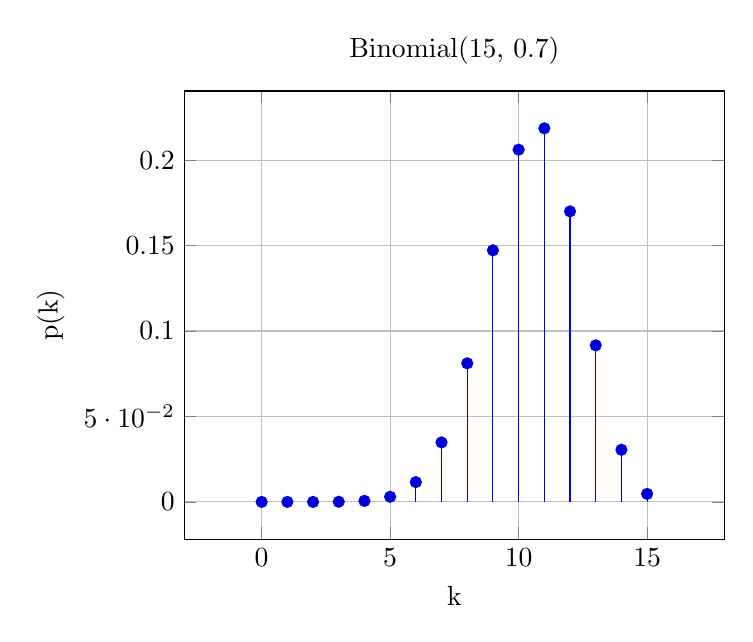
\begin{tikzpicture}
		\begin{axis}[enlarge x limits=0.2, grid = both,
			xlabel = k, ylabel = p(k), title = {Binomial(15, 0.7)}]
			\addplot+[ycomb] plot coordinates {( 0 , 0.0 ) ( 1 , 0.0 ) ( 2 , 0.0 ) ( 3 , 0.0001 ) ( 4 , 0.0006 ) ( 5 , 0.003 ) ( 6 , 0.0116 ) ( 7 , 0.0348 ) ( 8 , 0.0811 ) ( 9 , 0.1472 ) ( 10 , 0.2061 ) ( 11 , 0.2186 ) ( 12 , 0.17 ) ( 13 , 0.0916 ) ( 14 , 0.0305 ) ( 15 , 0.0047 ) };  
		\end{axis} 
	\end{tikzpicture}
\end{figure}


The two defining parameters of a Binomial RV are $ (n, p) $ where $ n $ is the number of trials and $ p $, the probability of each trial being independently a success.

\begin{align}
	P \left\{X = i\right\} &= \binom{n}{i}\ p^i \ (1-p)^{n-i}
\end{align}

Proving the normalization constraint requires the binomial theorem,
\begin{align}
	[p + (1-p)]^n &= 1^n = 1 \nonumber \\
	%
	\sum\limits_{i=0}^{n} P \left\{X = i\right\} &= \sum\limits_{i=0}^{n} \binom{n}{i}\ p^i \ (1-p)^{n-i}  = 1
\end{align}

Using the fact that the $ \mathbb{E}[\sum X] $ when the RVs are independent, reduces to $ \sum \mathbb{E}[X] $, and a similar rule for the variance,

\begin{align}
	\mathbb{E}[X] &= np \\
	%
	\mathrm{Var}(X) &= np(1-p)
\end{align}

If $ X_1, X_2 $ are two binomial RVs with parameters $ (n_1, p) $ and $ (n_2, p) $, then the RV $ X = X_1 + X_2 $ is also a binomial RV with parameters $ (n_1 + n_2, p) $ 

\textbf{Poisson RV} : Consider an RV that takes on non-negative integer values along with a parameter $ \lambda > 0 $, whose PMF is given by


\begin{align}
	P \left\{X = i\right\} &= e^{-\lambda}\ \frac{\lambda^i}{i!}
\end{align}

Using the Taylor series expansion of the exponential function, the normalization constraint is proved as follows,


\begin{align}
	e^x &= 0 + 1 + \frac{x^2}{2!} + \frac{x^3}{3!} + \dots \nonumber \\
	%
	\sum\limits_{i=0}^{\infty} P \left\{X = i\right\} &= e^{-\lambda} \left(\sum\limits_{i=0}^{\infty} \frac{\lambda^i}{i!}\right) = e^{-\lambda} \ e^{\lambda} = 1
\end{align}

\begin{figure}[!h]
	\centering
	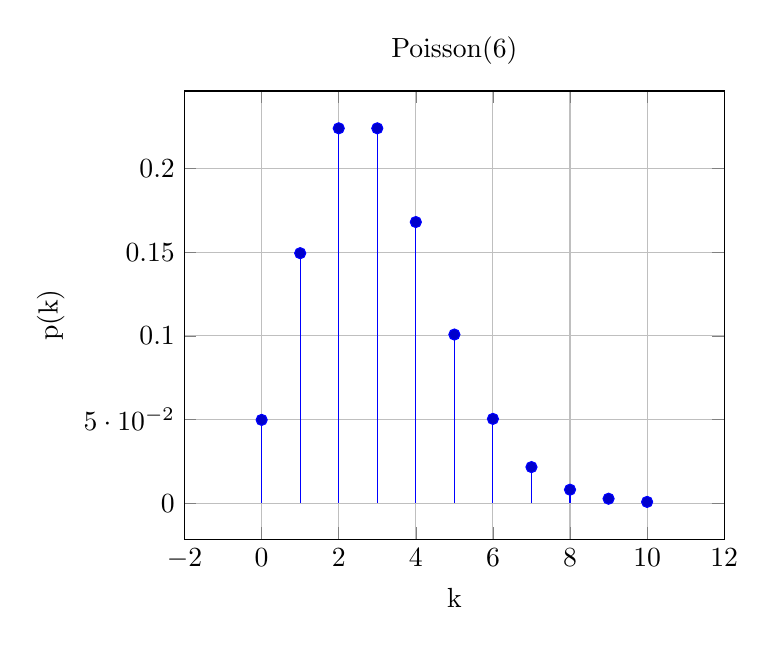
\begin{tikzpicture}
		\begin{axis}[enlarge x limits=0.2, grid = both,
			xlabel = k, ylabel = p(k), title = {Poisson(6)}]
			\addplot+[ycomb] plot coordinates {( 0 , 0.0498 ) ( 1 , 0.1494 ) ( 2 , 0.224 ) ( 3 , 0.224 ) ( 4 , 0.168 ) ( 5 , 0.1008 ) ( 6 , 0.0504 ) ( 7 , 0.0216 ) ( 8 , 0.0081 ) ( 9 , 0.0027 ) ( 10 , 0.0008 ) };  
		\end{axis} 
	\end{tikzpicture}
\end{figure}

Using the derivatives of the moment-generating function $ \phi(t) $, gives the mean and variance,

\begin{align}
	\phi(t) &= \mathbb{E}[e^{tX}] = \exp\left\{\lambda (e^t - 1)\right\}\\
	%
	\mathbb{E}[X] &= \lambda \\
	%
	\mathrm{Var}(X) &= \lambda
\end{align}

In the limit of $ n $ very large and $ p $ very small for a binomial RV with parameters $ (n, p) $, it can be approximated using a Poisson RV with parameter $ \lambda = np $.

\begin{align}
	P \left\{X = i\right\}\ =\ \binom{n}{i}\ p^i\ (1-p)^{n-i}\ \approxeq\ e^{-np}\ \frac{(np)^i}{i!}
\end{align}

An evern more general result, uses $ n $ independent trials each with probability of success $ p_i \ \forall\ i \in \left\{1, \dots, n\right\}$, with the condition that $ n $ is large and all of the $ p_i $ are small. The Poisson RV approximation can then me made with parameter $ \lambda = \sum p_i $.

Weak independence is measured by the conditional probability of one event succeeding given another has already succeeded. If these two values are approximately equal, then this approximation applies.

If $ X_1, X_2 $ are independently Poisson distributed with parameters $ \lambda_1, \lambda_2 $, then their sum $ X = X_1 + X_2 $ is also Poisson distributed with parameter $ \lambda_1 + \lambda_2 $. Since the moment generating function of a distribution uniquely determines it,

\begin{align}
	\phi (t) &= \mathbb{E}[e^{tX}] = \mathbb{E}[e^{t(X_1 + X_2)}] \nonumber \\
	%
	&= \mathbb{E}[e^{tX_1}] \mathbb{E}[e^{tX_2}] \nonumber \\
	%
	&= \exp\left\{(\lambda_1 + \lambda_2) (e^t - 1)\right\}
\end{align}

As an extension of the above, consider a total of $ N $ events, of which $ N_1, N_2 $ represent the number of events of types 1 and 2, with probabilities $ p $ and $ 1-p $ respectively. Also, $ N = N_1 + N_2 $.

If $ N $ is Poisson distributed with mean $\lambda$, then $ N_1, N_2 $ are also Poisson distributed with mean $ p\lambda $ and $ (1-p)\ \lambda $ respectively. This easily extends to more than two possible event types.

\begin{align}
	P\left\{N = n+m\right\} &= e^{-\lambda} \ \frac{\lambda^{n+m}}{(n+m)!} \nonumber \\
	%
	P\left\{N_1 = n\right\} &= e^{-p\lambda} \ \frac{(p\lambda)^{n}}{(n)!} \nonumber \\
	%
	P\left\{N_2 = m\right\} &= e^{-(1-p)\lambda} \ \frac{((1-p)\lambda)^{m}}{(m)!}
\end{align}

\textbf{Hypergeometric RV} : Consider a set of $ N+M $ objects of which $ N $ are acceptable and $ M $ defective. Let an experiment involve choosing $ n $ random objects out of $ N+M $, and then measure the number of acceptable objects picked using the RV $ X $.

$ X \in \left\{0, 1, \dots, \min(n, N) \right\} $, as the number of acceptable objects picked cannot exceed $ N $. This is a hypergeometric RV with PMF given by,

\begin{align}
	P \left\{X = i\right\} &= \ddfrac{\binom{N}{i}\ \binom{M}{n-i}}{\binom{N+M}{n}}
\end{align}

The parameters are $ (N, M, n) $, with the RV taking on non-negative integer values. If the proportion of acceptable objects is $ p $, then,

\begin{align}
	\mathbb{E}[X] &= \frac{nN}{N+M} = np \\
	%
	\mathrm{Var}(X) &= \frac{nNM}{(N+M)^2}\ \left(1 - \frac{n-1}{N+M-1}\right) \nonumber \\
	%
	&=  np\ (1-p)\ \left(1 - \frac{n-1}{N+M-1}\right)
\end{align}

Notice from the variance that the hypergeometric distribution converges to a binomial distribution in the limit $ N+M \to \infty $ and thus $ n \lll N $.

Consider two binomial RVs $ X, Y $ with parameters $ (n, p) $ and $ (m, p) $ respectively. The PMF of $ X $, given $ X+Y = k $ is given by,

\begin{align}
	P \left\{X = i\ |\ X+Y = k\right\} &= \ddfrac{\binom{n}{i}\ \binom{m}{k-i}}{\binom{n+m}{k}}
\end{align}

The denominator uses the fact that $ X+Y $ is also binomial with paramters $ (n+m, p) $, and the expression measures the probability that $ i $ out of the $ k $ successes were contributed by the RV $ X $.

This turns out to be a hypergeomtric RV measuring how many out of $ k $ objects picked were of type $ X $.


\textbf{Uniform RV} : Consider a continuous RV over the closed interval $ \left[\alpha, \beta\right] $, with PDF given by

\begin{align}
	f(x) &= \frac{1}{\beta - \alpha} & \text{if}\ x \in \left[\alpha, \beta\right] \\
	%
	f(x) &= 0 & \text{otherwise} \nonumber
\end{align}

The normalization constriant is easily proven using the Riemann integration of a continuous function.

\begin{align}
	P \left\{a < X < b\right\} &= \int\limits_{a}^{b} f(x)\ \mathrm{d} x = \frac{b - a}{\beta - \alpha} \\
	%
	P \left\{-\infty < X < \infty\right\} &= \int\limits_{-\infty}^{\infty} f(x)\ \mathrm{d} x = 1 \nonumber
\end{align}

Using simple polynomial integrations,

\begin{align}
	\mathbb{E}[X] &= \frac{\alpha + \beta}{2} \\
	%
	\mathrm{Var}(X) &= \frac{(\beta - \alpha)^2}{12} 
\end{align}


By computer science convention, a \textit{random number} is a uniformly distributed real number in the range $ [0, 1] $. A simple linear transformation $ Y = aX + b $ can be used to rescale this random number to the domain $ [b, a+b] $.

An important application of uniform RV sampling is Monte Carlo simulations, often used to estimate a parameter by performing a large number of experiments and using a frequentist approach to assign probabilities.

\textbf{Normal RV} : The most consistent distribution underlying real-world datasets, and as a result the most well-studied. This was originally introduced as an approximation to binomial distributions with extremely large $ n $. Using the mean and variance as parameters, the PDF for $ X \sim \mathcal{N}(\mu, \sigma^2) $ is defined as

\begin{align}
	f(x) = \frac{1}{\sqrt{2 \pi \sigma^2}} \exp \left[\frac{- (x - \mu)^2}{2\sigma^2}\right] \qquad \forall \quad x \in \mathbb{R}
\end{align}

This distribution is also called a bell curve. It is symmetric about $ \mu $, which is also its maximum.

\begin{align}
	\mathbb{E}[X] &= \mu \\
	%
	\mathrm{Var}(X) &= \sigma^2 \\
	%
	\mathbb{E}[aX + b] &= a\ \mu + b \nonumber \\
	%
	\mathrm{Var}(aX + b) &= a^2 \ \sigma^2 \nonumber 
\end{align}

\textit{Standard normal RV} : A normal RV with mean 0 and variance 1. Any normal RV $ X $ can be converted into a standard normal RV ($ \Phi $), using the transform $ Z = (X - \mu) / \sigma$

\begin{align}
	X &\sim \mathcal{N}(\mu, \sigma^2) \nonumber \\
	%
	Z &\sim \mathcal{N}(0, 1) \qquad \text{using} \qquad Z = \frac{X - \mu}{\sigma}
\end{align}

\begin{figure}[H]
	\centering
	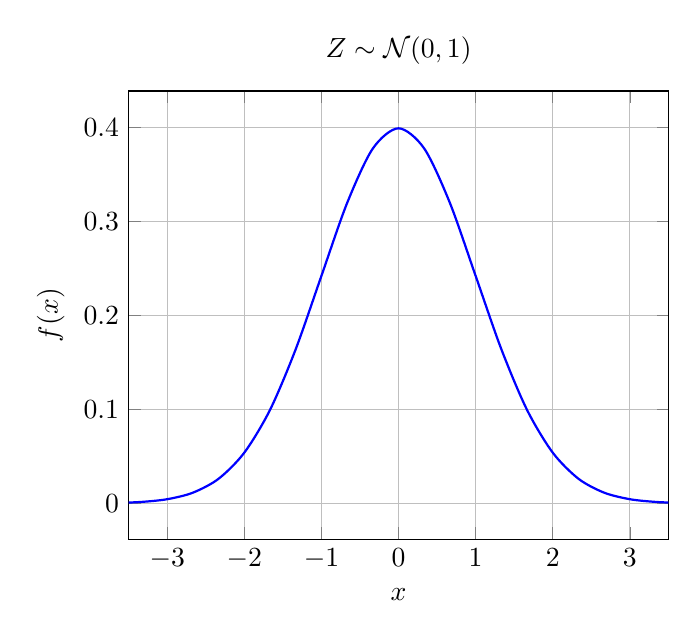
\begin{tikzpicture}
		\begin{axis}[xlabel=$x$, grid = both, xmin = -3.5, xmax = 3.5, ylabel = {$f(x)$}, title = {$ Z \sim \mathcal{N}(0, 1) $}]
			\addplot[thick, smooth, draw=blue][name path = f2, domain = -4:4]{(1/sqrt(2*pi)*exp(-x*x*0.5))};
		\end{axis}
	\end{tikzpicture}
\end{figure}

The numerical value of the standard normal RV $ (\Phi) $ has historically been computed using approximations and the CDF tabulated to a high degree of precision. Such a reference table is used to actually assign probabilities to $ \Phi $ 

\begin{align}
	\Phi(x) &= \int\limits_{-\infty}^{x} \frac{1}{\sqrt{2 \pi}} \exp \left(\frac{-y^2}{2}\right)\ \mathrm{d}y \\
	%
	P\left\{X < b\right\} &= P \left\{\frac{X - \mu}{\sigma} < \frac{b - \mu}{\sigma}\right\} = \Phi \left\{\frac{b - \mu}{\sigma}\right\} \\
	%
	\Phi(-x) &= 1 - \Phi(x)
\end{align}

The moment generating function of a normal RV uses the result for a standard normal RV.

\begin{align}
	\phi_Z (t) &= \mathbb{E}[e^{tZ}] = \exp\left(\frac{t^2}{2}\right)	  \\
	%
	\phi_X (t) &= \mathbb{E}[e^{t\mu}\ e^{t \sigma Z}] = \exp\left(\mu t + \frac{\sigma^2 t^2}{2}\right)
\end{align}

This also leads to the fact that the sum of independent normal RVs is also a normal RV. Consider a set of normal RVs $ \left\{X_i\right\} $ with mean and variance $ \left\{\mu_i\right\},\ \left\{\sigma^2_i\right\} $ respectively. From the moment-generating function,

\begin{align}
	\mathbb{E}[e^{tX}] &= \prod_{i=1}^{n} \mathbb{E}[e^{tX_i}] \nonumber \\
	%
	\mu &= \sum\limits_{i=1}^{n} \mu_i \qquad \text{and} \qquad \sigma^2 = \sum\limits_{i=1}^{n} \sigma_i^2
\end{align}

\textit{Percentile and z-score} : By convention, $ \alpha $ and $ z_\alpha $ are called the \textit{p-value} and \textit{z-score} respectively. The $ 100 \alpha $ percentile of a standard normal RV is that value $ x = z_\alpha $ for which,

\begin{align}
	P \left\{Z > z_\alpha\right\} &= 1 - \Phi(z_\alpha) = \alpha
\end{align}

\begin{figure}[H]
	\centering
	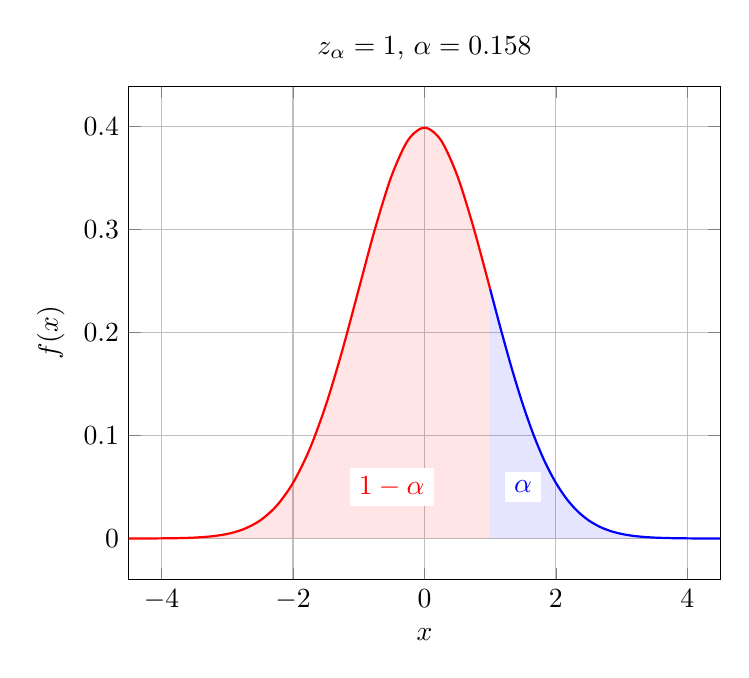
\begin{tikzpicture}
		\begin{axis}[width = 0.75\textwidth,xlabel=$x$, ylabel=$ f(x) $, grid = both, xmin = -4.5, xmax = 4.5, title = {$z_\alpha = 1$, $ \alpha = 0.158 $}]
			\addplot[thick, smooth, draw=red][name path = f1, domain = -5:1]{(1/sqrt(2*pi)*exp(-x*x*0.5))};
			\addplot[thick, smooth, draw=blue][name path = f2, domain = 1:5]{(1/sqrt(2*pi)*exp(-x*x*0.5))};
			
			\path[name path=axis1] (axis cs:-5,0) -- (axis cs:1,0);
			\path[name path=axis2] (axis cs:1,0) -- (axis cs:5,0);
			
			\addplot [thick,color=red,fill=red, fill opacity=0.1] fill between[of=f1 and axis1,];
			\addplot [thick,color=red,fill=blue, fill opacity=0.1] fill between[of=f2 and axis2,];
			
			\node[color=blue, fill=white] at (axis cs: 1.5,.05) {$ \alpha $};
			\node[color=red, fill=white] at (axis cs: -0.5,.05) {$ 1 - \alpha $};
			
		\end{axis}
	\end{tikzpicture}
\end{figure}


\textbf{Exponential RV} :  Consider a continuous RV defined over the real line with PDF and CDF given by

\begin{align}
	f(x) &= \lambda\ e^{-\lambda x} & \text{if}\ x \in \left[0, \infty\right) \\
	%
	f(x) &= 0 & \text{otherwise} \nonumber
\end{align}


\begin{figure}[H]
	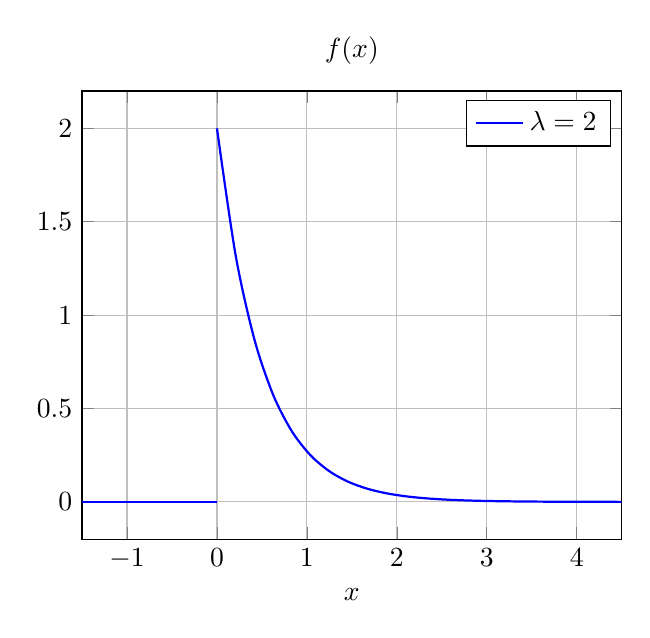
\begin{tikzpicture}
		\begin{axis}[xlabel=$x$, grid = both, xmin = -1.5, xmax = 4.5, title = {$f(x)$}]
			\addplot[thick, smooth, draw=blue][name path = f1, domain = -2:0]{0};
			\addplot[thick, smooth, draw=blue][name path = f1, domain = 0:5]{2*exp(-2*x)};
			\addlegendentry{$ \lambda = 2$}
		\end{axis}
	\end{tikzpicture}
	%
	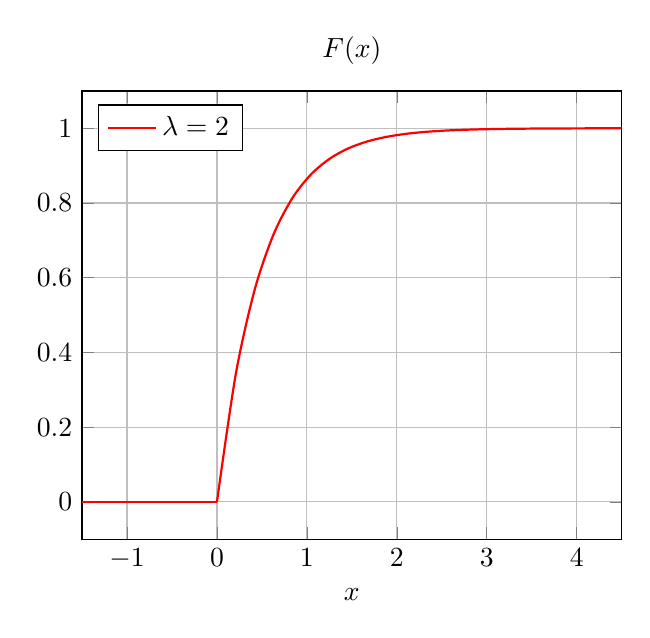
\begin{tikzpicture}
		\begin{axis}[xlabel=$x$, grid = both, xmin = -1.5, xmax = 4.5, title = {$F(x)$}, legend pos = north west]
			\addplot[thick, smooth, draw=red][name path = f1, domain = -2:0]{0};
			\addplot[thick, smooth, draw=red][name path = f1, domain = 0:5]{1 - exp(-2*x)};
			\addlegendentry{$ \lambda = 2$}
		\end{axis}
	\end{tikzpicture}
\end{figure}


The parameter $ \lambda $ , called the \textit{rate}, solely defines the exponential RV with a CDF,

\begin{align}
	F(x) &= 1 - e^{-\lambda x} \qquad \forall \ x \geq 0
\end{align}

The exponential distribution if observed most commonly as the distribution of time intervals between successive occurrences of natural events. The moment-generating function gives the mean and variance as follows

\begin{align}
	\phi(t) &= \frac{\lambda}{\lambda - t} \qquad \forall\ t < \lambda \\
	%
	\mathbb{E}[X] &= \frac{1}{\lambda} \\
	%
	\mathrm{Var}(X) &= \frac{1}{\lambda^2}
\end{align}

An important property exclusive to the exponential function is that it is \textit{memoryless}, or \textit{self-similar} across time. This is mathematically represented as

\begin{align}
	P \left\{X > t+s\ |\ X > t \right\} &= P \left\{X > s \right\} \qquad \forall \ s, t\geq 0
\end{align}

The probability of an item functioning for $ s $ additional time does not depend on the fact that it has functioned for $ t $ time already.

The minimum of a set of independent exponential RVs $ \left\{X_i\right\} $ with parameters $ \left\{\lambda_i\right\} $ is also an exponential RV. This is easily understood as the lifetime of a system with many components all of which are necessary for it to function.

\begin{align}
	P \left\{\mathrm{min}(X_1, X_2, \dots, X_n) > x\right\} &= e^{-\lambda x} \nonumber \\
	%
	\lambda &= \sum_{i=1}^{n} \lambda_i
\end{align}

An independent exponential RV transforming as $ X \to cX $ causes the rate to change as $ \lambda \to \lambda/c $.

\textbf{Poisson process} : Consider a process where events happen randomly such that $ N(t) $ denotes the number of events in the time $ [0, t] $. This is a Poisson process with \textit{rate} $ \lambda $, if

\begin{itemize}
	\item $ N(0) = 0 $, with $ t = 0 $ denoting the start of the process.
	
	\item Disjoint time intervals have an independent number of events occurring in them.
	
	\item The number of events in a given interval has a distribution depending only on the length of the interval.
	
	\item In the limit of a small time interval of length $ h \to 0 $, the probability of event occurrence
	
	\begin{align}
		P \left\{N(h) = 1\right\} &\approx \lambda h \nonumber \\
		%
		P \left\{N(h) \geq 2\right\} &\approx 0
	\end{align}
\end{itemize}

The distribution of the number of events occurring in any interval of length $ t $ in a Poisson process is a Poisson RV with parameter $ \lambda t $.

\begin{align}
	P \left\{N(t) = k\right\} &= e^{-\lambda t} \ \frac{(\lambda t)^k}{k!}
\end{align}

For a Poisson process, let $ Y_n $ denote the time interval between the $ (n-1)^{th} $ and $ n^{th} $ events for all $ n > 1 $. This set $ \left\{Y_n\right\} $ is called \textit{inter-arrival time}. Then, the set $ Y_n $ are all independent RVs having an exponential distribution with parameter $ \lambda $ 

\textbf{Pareto RV} : Using the self-similarity of the exponential RV, the Pareto distribution is used to exmaine the distribution of income among a population and to identify what proportion of the total income earned by a population is contributed by the top earners.

Consider an exponential RV $ X $ with rate $ \lambda $. The Pareto RV with minimum parameter $ \alpha $ and index parameter $ \lambda > 0$, is given by

\begin{align}
	Y &= \alpha\ e^{X} \\
	%
	X &= \lambda\ e^{-\lambda x} & \text{if}\ x \in \left[0, \infty\right) \nonumber
\end{align}

This RV is constrained by $ Y \geq \alpha $. The CDF of the Pareto distribution is

\begin{align}
	P \left\{Y > y\right\} &= \left(\frac{\alpha}{y}\right)^\lambda \nonumber \\
	%
	F_Y(y) &= 1 - \left(\frac{\alpha}{y}\right)^\lambda \qquad \forall \  y \geq \alpha \\
	%
	f_Y(y) &= \frac{\lambda}{y}\ \left(\frac{\alpha}{y}\right)^\lambda \qquad \forall \  y \geq \alpha
\end{align}

\begin{figure}[H]
	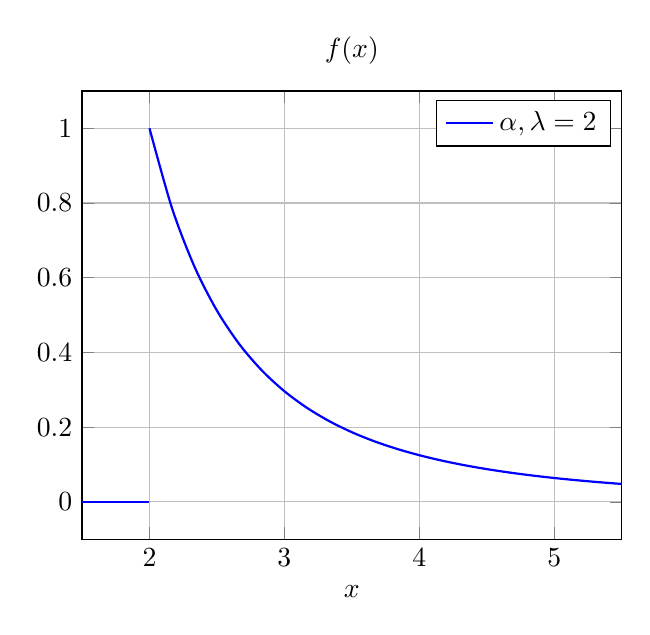
\begin{tikzpicture}
		\begin{axis}[xlabel=$x$, grid = both, xmin = 1.5, xmax = 5.5, title = {$f(x)$}]
			\addplot[thick, smooth, draw=blue][name path = f1, domain = 0:2]{0};
			\addplot[thick, smooth, draw=blue][name path = f1, domain = 2:6]{8/(x^(3))};
			\addlegendentry{$ \alpha, \lambda = 2$}
		\end{axis}
	\end{tikzpicture}
	%
	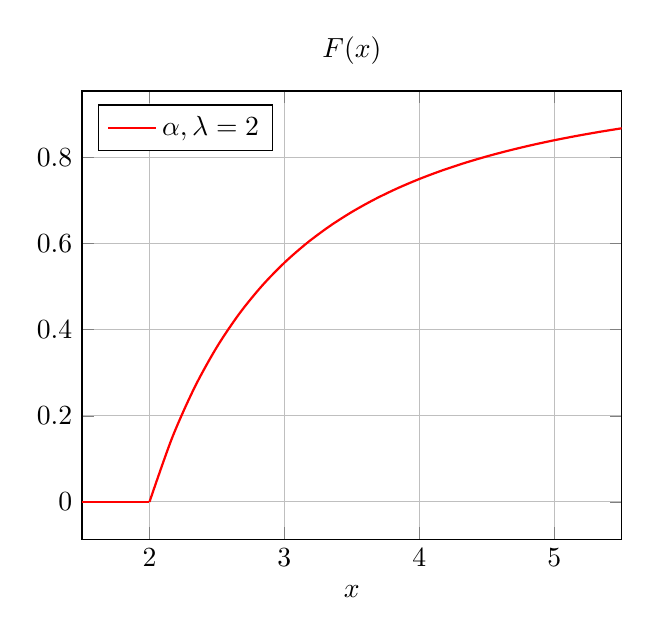
\begin{tikzpicture}
		\begin{axis}[xlabel=$x$, grid = both, xmin = 1.5, xmax = 5.5, title = {$F(x)$}, legend pos = north west]
			\addplot[thick, smooth, draw=red][name path = f1, domain = 0:2]{0};
			\addplot[thick, smooth, draw=red][name path = f1, domain = 2:6]{1 - (2/x)^2};
			\addlegendentry{$ \alpha, \lambda = 2$}
		\end{axis}
	\end{tikzpicture}
\end{figure}

The expected value is finite only for $ \lambda > 1 $,

\begin{align}
	\mathbb{E}(Y) &= \alpha \ \frac{\lambda}{\lambda - 1 }
\end{align}

As a result of the self-similarity of the exponential distribution, the Pareto RV is also self-similar. Given the condition $ Y > y_0 $ for some $ y_0 > \alpha $, this conditional distribution is also Pareto with parameters $ y_0 $ and $ \lambda $.

\begin{align}
	P \left\{Y > y\ |\ Y > y_0 \right\} = \left(\frac{y_0}{y}\right)^\lambda
\end{align}

\textbf{Gamma distribution} : Consider the gamma function $ \Gamma(x) $ defined by an integral which can be recursively related to itself.

\begin{align}
	\Gamma(\alpha) &= \int\limits_{0}^{\infty} e^{-y}\ y^{\alpha -1}\ \mathrm{d}y \\
	%
	\Gamma(\alpha) &= (\alpha - 1)\ \Gamma(\alpha - 1)
\end{align}

For the special case of integer values of $ \alpha $, and using $ \Gamma(1) = 1 $,
\begin{align}
	\Gamma(n) &= (n - 1)\ \Gamma(n - 1) \nonumber \\
	%
	\Gamma(n) &= (n-1)!	
\end{align}

The Gamma RV with parameters $ \alpha, \lambda > 0 $, is now defined using the PDF,

\begin{align}
	f(x) &= \lambda\ e^{- \lambda x}\ \frac{(\lambda x)^{\alpha-1}}{\Gamma(\alpha)} \qquad \forall\ x \geq 0 \\
	%
	&= 0 \qquad \text{otherwise} \nonumber
\end{align}

\begin{figure}[H]
	\centering
	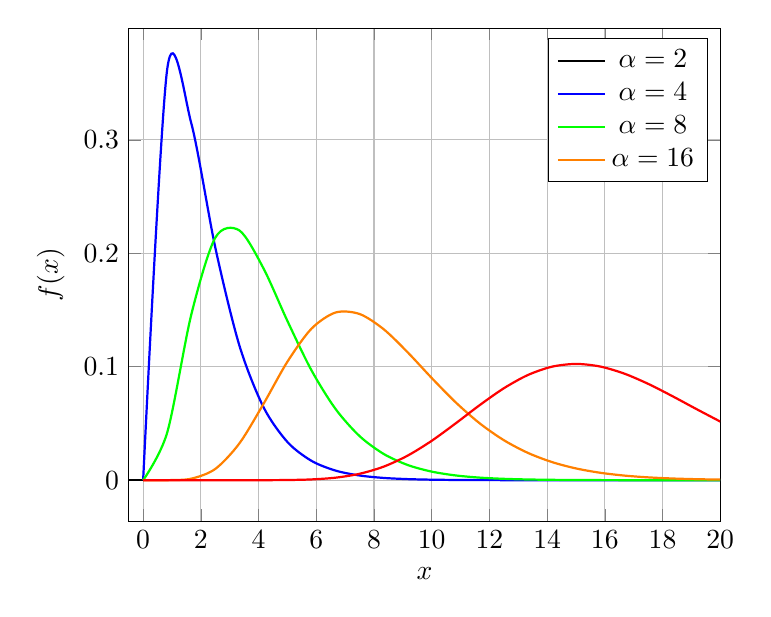
\begin{tikzpicture}
		\begin{axis}[width = 0.75\textwidth,xlabel=$x$, ylabel=$ f(x) $, grid = both, xmin = -0.5, xmax = 20]
			\addplot[thick, smooth, draw=black][name path = f1, domain = -1:0]{0};
			\addplot[thick, smooth, draw=blue][name path = f2, domain = 0:20]{e^(-x)*x};
			\addplot[thick, smooth, draw=green][name path = f3, domain = 0:20]{e^(-x)*(x^3)/6};
			\addplot[thick, smooth, draw=orange][name path = f4, domain = 0:20]{e^(-x)*(x^7)/5040};
			\addplot[thick, smooth, draw=red][name path = f5, domain = 0:20]{e^(-x)*(x^15)/1307674368000};
			\legend{$ \alpha = 2 $, $ \alpha = 4 $, $ \alpha = 8 $, $ \alpha = 16 $}
		\end{axis}
	\end{tikzpicture}
\end{figure}



The moment-generating function gives the mean and variance using

\begin{align}
	\phi(t) &= \left(\frac{\lambda}{\lambda - t}\right)^{\alpha} \\
	%
	\mathbb{E}[X] &= \frac{\alpha}{\lambda} \\
	%
	\mathrm{Var}(X) &= \frac{\alpha}{\lambda^2}
\end{align}

Using the moment-generating function above, the sum of many independent Gamma RVs $ \left\{X_i\right\} $ with parameters $ \left\{\alpha_i\right\} $ and a shared $ \lambda $, then their sum $ X = \sum X_i $ is also a Gamma RV with parameters $ \sum \alpha_i $ and $\lambda$.

This result further simplifies when $ \alpha = 1 $, making the Gamma RVs reduce to exponential RVs with the same rate parameter $ \lambda $. The sum of $ n $ independent exponential RVs $ \left\{X_i\right\} $ with a shared rate $ \lambda $, is a Gamma RV with parameters $ (n, \lambda) $.

Note the effect of multiplying a Gamma RV by a scalar. Let $ X $ be a Gamma RV which is multiplied by scalar $ b $, Now the moment-generating function of the new RV $ bX $ is

\begin{align}
	\mathbb{E}[e^{tX}] &= \left(\frac{\lambda}{\lambda - t}\right)^\alpha \nonumber \\
	%
	\mathbb{E}[e^{t\ bX}] &= \mathbb{E}[e^{bt\ X}] = \left(\frac{\lambda}{\lambda - bt}\right)^\alpha = \left(\frac{\lambda / b}{\lambda / b - t}\right)^\alpha \nonumber \\
	%
	bX &\sim \Gamma(\alpha, \lambda / b)  \qquad \text{if} \qquad X \sim \Gamma(\alpha, \lambda)
\end{align}

\textbf{Chi-square distribution} : Consider a set of independent standard normal RVs $ \left\{Z_i\right\} $. Then the RV defined as $ X \sim \chi_n^2 $ is given by

\begin{align}
	X = Z_1^2 + Z_2^2 + \dots + Z_n^2
\end{align}

$ X $ is a chi-squared RV with $ n $ \textit{degrees of freedom}. Similar to the p-value from the normal RV, $ \chi_{\alpha, n}^2 $ is defined as follows and tabulated using approximate computations.

\begin{align}
	P \left\{X \geq \chi_{\alpha, n}^2 \right\} = \alpha
\end{align}

The equivalence of the chi-squared and Gamma distributions can be seen through the moment-generating functions 

\begin{align}
	\phi(t) &= (1-2t)^{-n/2} \\
	%
	\phi(t) &= \left(\frac{1/2}{1/2 - t}\right)^{n/2} \nonumber
\end{align}

Thus, a chi-squared RV with $ n $ degrees of freedom is the same as a Gamma distribution with parameters $ (n/2, 1/2) $.

\begin{align}
	\mathbb{E}[X] &= \frac{n/2}{1/2} = n \\
	%
	\mathrm{Var}(X) &= \frac{n/2}{(1/2)^2} = 2n
\end{align}

\textbf{t-distribution} : Using a standard normal RV $ Z $ and a chi-square RV $ \chi_n^2 $ with $ n $ degrees of freedom, the t-distribution is defined as,

\begin{align}
	T_n = \frac{Z}{\sqrt{\chi_n^2 / n}}
\end{align}

The t-distribution is also symmetric about $ x=0 $ like $ Z $, but with longer tails. It increasingly resembles $ Z $ as $ n \to \infty $. To prove this, use the weak law of large numbers on the denominator above.

\begin{align}
	\mathbb{E}[X] &= 0 \qquad n>1 \\
	%
	\mathrm{Var}(X) &= \frac{n}{n-2} \qquad n>2
\end{align}

Similar to the p-value from the normal RV, $ t_{\alpha, n} $ is defined as follows and tabulated using approximate computations.

\begin{align}
	P \left\{T_n \geq t_{\alpha, n} \right\} &= \alpha \\
	%
	t_{1-\alpha, n} &= -t_{\alpha, n} \nonumber
\end{align}

\textbf{F-distribution} : Let $ \chi_n^2, \chi_m^2 $ be chi-square RVs with $ n, m $ degrees of freedom respectively. Then,

\begin{align}
	F_{n,m} = \frac{\chi_n^2 / n}{\chi_m^2 / m}
\end{align}

is an F-distribution with$ n,m $ degrees of freedom.

Similar to the p-value from the normal RV, $ F_{\alpha, n, m} $ is defined as follows and tabulated using approximate computations.

\begin{align}
	P \left\{F_{n,m} \geq F_{\alpha, n, m} \right\} &= \alpha \\
\end{align}

\newpage


%	\chapter{Distributions of Sampling Statistics}

\begin{enumerate}
	
	\item 
		\begin{enumerate}
			\item Let $ Y = (X_1 + X_2) / 2 $. This gives the following joint PMF for $ Y $,
			\begin{table}[H]
				\centering
				\begin{tabular}{@{}rrrrr@{}}
					\toprule
					&     $ X_1 =  $0 &     $ X_1 =  $1 &    $ X_1 =  $2 &     $ X_1 =  $3 \\
					\midrule
					$ X_2 =  $0 &  0.04 &  0.06 &  0.0 &  0.10 \\
					$ X_2 =  $1 &  0.06 &  0.09 &  0.0 &  0.15 \\
					$ X_2 =  $2 &  0.00 &  0.00 &  0.0 &  0.00 \\
					$ X_2 =  $3 &  0.10 &  0.15 &  0.0 &  0.25 \\
					\bottomrule
				\end{tabular}
			\end{table}
			
			\begin{table}[H]
				\centering
				\begin{tabular}{@{}rrrrr@{}}
					\toprule
					$ i $ &     $P\left\{Y = i\right\}$ \\
					\midrule
					0 &  0.04  \\
					1/2 &  0.12  \\
					1 &  0.09  \\
					3/2 &  0.20  \\
					2 & 0.30 \\
					5/2 & 0.00 \\
					3 & 0.25 \\
					\bottomrule
				\end{tabular}
			\end{table}
			
			\item \begin{align}
				\mathbb{E}[Y] &= \sum\limits_{i} i\ \times P\left\{Y = i\right\} = 1.8 \\
				%
				\mathbb{E}[Y^2] &= \sum\limits_{i} i^2\ \times P\left\{Y = i\right\} = 4.02 \nonumber \\
				%
				\mathrm{Var}(Y) &= 4.02 - (1.8)^2 = 0.78
			\end{align}
			
			Alternatively, using the new sample mean and variance formulae,
			
			\begin{align}
				\mathbb{E}[X_i] &= 1.8 & \mathrm{Var}(X_i) &= 4.8 - 1.8^2 = 1.56 \\
				%
				\mathbb{E}[\overline{X}] &= \mathbb{E}[X_i] = 1.8  &\mathrm{Var}(\overline{X}) &= \mathrm{Var}(X_i) / 2 = 0.78
			\end{align}
			
			\item Let $ Z = (X_1 + X_2 + X_3) / 3 $. The PMF of $ Z $ is given by
			\begin{table}[H]
				\centering
				\begin{tabular}{@{}rrrrr@{}}
					\toprule
					$ i $ &     $P\left\{Z = i\right\}$ \\
					\midrule
					0 &  0.008  \\
					1/3 &  0.036  \\
					2/3 &  0.054  \\
					1 &  0.087  \\
					4/3 & 0.18 \\
					5/3 & 0.135 \\
					2 & 0.15 \\
					7/3 & 0.225 \\
					8/3 & 0 \\
					3 & 0.125 \\
					\bottomrule
				\end{tabular}
			\end{table}
			
			\item Using the new sample mean and variance formulae,
			
			\begin{align}
				\mathbb{E}[X_i] &= 1.8 & \mathrm{Var}(X_i) &= 4.8 - 1.8^2 = 1.56 \\
				%
				\mathbb{E}[\overline{Z}] &= \mathbb{E}[X_i] = 1.8  &\mathrm{Var}(\overline{Z}) &= \mathrm{Var}(X_i) / 3 = 0.52
			\end{align}
		\end{enumerate}
	
	
	\item 10 fair dice are rolled. Let the dice be $ \left\{X_i\right\} $. Now, $ Y = \sum_{i} X_i  $
	
	
		\begin{align}
			\mathbb{E}[X_i] &= 3.5 		& \mathrm{Var}(X_i) &= 91/6 - 49/4 = 35/12 \nonumber \\
			%
			\mathbb{E}[Y] &= 35 		& \mathrm{Var}(Y) &= 350/12 
		\end{align}
		
		Using central limit theorem with continuity correction,
		\begin{align}
			P\left\{29.5 \leq Y \leq 40.5 \right\} &= P\left\{\frac{29.5 - 35}{\sqrt{350/12}} \leq Z \leq \frac{40.5 - 35}{\sqrt{350/12}}\right\} \nonumber \\
			%
			&= \Phi \left( \frac{40.5 - 35}{\sqrt{350/12}} \right) - \Phi\left(\frac{29.5 - 35}{\sqrt{350/12}}\right) = 0.6915
		\end{align}
	
	
	\item 16 independent standard uniform RV. Let $ Y = \sum X_i  $.
	
		\begin{align}
			P \left\{Y > 10 \right\} &= P \left\{ \overline{X} > 10/16 \right\} \nonumber \\
			%
			&= P \left\{ \frac{4\ (\overline{X} - 0.5)}{\sqrt{1/12}}> \frac{1/2}{\sqrt{1/12}} \right\} \nonumber \\
			%
			&= 1 - \Phi\left( \frac{1/2}{\sqrt{1/12}} \right) = 0.0416
		\end{align}
	
	
	\item 
		\begin{enumerate}
			\item Each bet is independent with probability of success $ p = 1/38 $. Let $ Y = \sum X_i $\\
			\begin{align}
				\mathbb{E}[X] &= 35 \times 1/38 + (-1) \times 37/38 = -1/19 \\
				%
				\mathbb{E}[X^2] &= 35^2 \times 1/38 + (-1)^2 \times 37/38 = 631/19 \nonumber \\
				%
				\mathrm{Var}(X) &= 630/19 = 33.16 \\
				%
				\mathbb{E}[Y] &= n\mu \qquad \mathrm{Var}(Y) = n\sigma^2 \nonumber \\
				%
				P \left\{ Y > 0 \right\} &= 1 - \Phi \left( \frac{0 - n\mu}{\sqrt{n\sigma^2}} \right) \nonumber
			\end{align}
			
			\item The fact that the expected value of a single bet is negative means that it is more difficult to remain positive as the number of bets increases.
			\begin{align}
				n = 34 &\to P \left\{ Y > 0 \right\} = 0.4787 \nonumber \\
				%
				n = 1000 &\to P \left\{ Y > 0 \right\} = 0.3863 \nonumber \\
				%
				n = 100000 &\to P \left\{ Y > 0 \right\} = 0.0019 \nonumber
			\end{align}
		\end{enumerate}
	 
	
	\item $ X_i $ is an RV with $ \mu = 1.5 $ and $ \sigma = 0.3 $. Assume \\
	
		\begin{enumerate}
			\item $ n = 50 $
			\begin{align}
				\mathbb{E}[Y] &= n\mu \qquad \mathrm{Var}(Y) = n\sigma^2 \nonumber \\
				%
				P \left\{ Y \leq 80 \right\} &= P \left\{Z \leq \frac{80 - n\mu}{\sqrt{n\sigma^2}} \right\} \nonumber \\
				%
				&= \Phi \left(\frac{80 - 75}{\sqrt{50\ (0.3)^2}}\right) = 0.9908
			\end{align}
			
			\item Assume snowfall on each day is independent.
			
			\item Assumption is bad since current weather events are usually dependent on the weather conditions of the past days.
			
		\end{enumerate}
	 
	
	\item 50 independent uniform RV in the range $ [-0.5, 0.5] $. Let $ Y = \sum X_i  $.
	
		\begin{align}
			P \left\{Y > 3 \right\} &= P \left\{ \overline{X} > 0.06 \right\} \nonumber \\
			%
			&= P \left\{ \frac{\sqrt{50}\ (\overline{X} - 0)}{\sqrt{1/12}}> \frac{0.06 \sqrt{50}}{\sqrt{1/12}} \right\} \nonumber \\
			%
			&= 1 - \Phi\left( \frac{0.06 \sqrt{50}}{\sqrt{1/12}} \right) = 0.0708 \nonumber \\
			%
			P \left\{|Y| > 3 \right\} &= 2 \times P \left\{Y > 3 \right\} = 0.1416
		\end{align}
	
	
	\item $ \mu = 7/2 $ and $ \sigma^2 = 35/12 $. Let $ n = 140 $ , Let $ Y = \sum X_i $\\
	
		\begin{align}
			P \left\{Y < 400 \right\} &= P \left\{ Z < \frac{(400 - 490)}{\sqrt{35/12 \times 140}} \right\} \nonumber \\
			%
			&= \Phi (-4.4538) \approx 0
		\end{align}
	
	
	\item $ \mathbb{E}[X_i] = 5 $ and $ \mathrm{Var}(X_i) = 2.25 $. Lifetime of 12 batteries has to be less than a year.
	Let $ Y = \sum^n_1 X_i $. At $ n = 12 $ ,
	
		\begin{align}
			P \left\{Y < 52 \right\} &= P \left\{ \overline{X} \leq 52/12 \right\} \nonumber \\
			%
			&= P \left\{ Z \leq \frac{\sqrt{12}\ (52/12 - 5)}{1.5} \right\} \nonumber \\
			%
			&= 0.0618 \nonumber 
		\end{align}
	
	
	\item $ \mu = 100 $ and $ \sigma = 20 $. Let $ n = 16 $ ,
	
		\begin{align}
			P \left\{\overline{X} < 104 \right\} &= P \left\{ Z < \frac{\sqrt{16}\ (104 - 100)}{20} \right\} \nonumber \\
			%
			&= \Phi (0.8) = 0.7881 \\
			%
			P \left\{98 < \overline{X} < 104 \right\} &= P \left\{ \frac{\sqrt{16}\ (98 - 100)}{20} < Z < \frac{\sqrt{16}\ (104 - 100)}{20} \right\} \nonumber \\
			%
			&= \Phi (0.8) - \Phi(-0.4) = 0.4436
		\end{align}
	
	
	\item $ \mu = 2.2 $ and $ \sigma = 0.3 $. Let $ n = 100 $ ,
	
		\begin{align}
			P \left\{\overline{X} > 3.1 \right\} &= P \left\{ Z > \frac{\sqrt{100}\ (3.1 - 2.2)}{0.3} \right\} \nonumber \\
			%
			&= 1 - \Phi (9/0.3) \approx 0  
		\end{align}
	
	
	\item $ \mu = 500 $ and $ \sigma = 80 $. Let $ n $ vary and check probability,
	
		\begin{align}
			P \left\{\overline{X} > 525 \right\} &= P \left\{ Z > \frac{\sqrt{n}\ (525 - 500)}{80} \right\} \\
			%
			n = 4 &\to P = 1 - \Phi(5/8) = 0.266 \nonumber \\
			%
			n = 16 &\to P = 1 - \Phi(5/4) = 0.1056 \nonumber \\
			%
			n = 36 &\to P = 1 - \Phi(15/8) = 0.0304 \nonumber \\
			%
			n = 64 &\to P = 1 - \Phi(2.5) = 0.00621 \nonumber 
		\end{align}
	
	
	\item $ \mu = 77$ and $ \sigma = 15 $. Let $ n = 25, 64 $ for the class average test scores $ Y, Z $ respectively,
	
		\begin{enumerate}
			\item \begin{align}
				P \left\{72 < Y < 82 \right\} &= P \left\{ \frac{\sqrt{25}\ (72 - 77)}{15} Z < \frac{\sqrt{25}\ (82 - 77)}{15} \right\} \nonumber \\
				%
				&= \Phi (5/3) - \Phi (-5/3) = 0.9044
			\end{align}
			
			\item \begin{align}
				P \left\{72 < Z < 82 \right\} &= P \left\{ \frac{\sqrt{64}\ (72 - 77)}{15} Z < \frac{\sqrt{64}\ (82 - 77)}{15} \right\} \nonumber \\
				%
				&= \Phi (8/3) - \Phi (-8/3) = 0.9923
			\end{align}
			
			\item Let $ W = Y - Z $, now, $ \mathbb{E}[W] = 0$, and $ \mathrm{Var}(W) = \sigma^2 (1/25 + 1/64) $\\
			\begin{align}
				P \left\{Y > Z \right\} &= P \left\{ W > 0 \right\} = \left\{ Z > \frac{(0 - 0)}{\sqrt{15*89/1600}} \right\} \nonumber \\
				%
				&= \Phi (0) = 0.5
			\end{align}
			
			\item The larger class has a smaller variance and is therefore, less likely have an average far from the mean. Thus, the smaller class is likelier to have a class average of 83.
		\end{enumerate}
	
	
	\item Binomial RV with $ n = 150$ and $ p = 0.6 $.
	
		\begin{enumerate}
			\item \begin{align}
				P \left\{X \leq 80 \right\} &=  \sum\limits_{k=0}^{80} \binom{150}{k}\ 0.6^k\ 0.4^{1-k}\nonumber \\
				%
				&= 0.05746
			\end{align}
			
			\item approximating using normal RV without continuity correction,
			\begin{align}
				P \left\{X \leq 80 \right\} &= P \left\{ \frac{X - np}{\sqrt{np(1-p)}} \leq \frac{(80 - 90)}{6} \right\} \nonumber \\
				%
				&= 0.04779
			\end{align}
			
			\item with continuity correction\\
			\begin{align}
				P \left\{X \leq 80.5 \right\} &= P \left\{ \frac{X - np}{\sqrt{np(1-p)}} \leq \frac{(80.5 - 90)}{6} \right\} \nonumber \\
				%
				&= 0.056673
			\end{align}
		\end{enumerate}
	
	
	\item Let $ A_2, A_3, A_4 $ denote the number of games that $ A $ wins against $ B, C, D $ respectively.
	
		\begin{enumerate}
			\item Looking at a table of the win probabilities,
			
			\begin{table}[H]
				\centering
				\begin{tabular}{@{}l|rrrr@{}}
					\toprule
					{} &     A &    B &    C &     D \\
					\midrule
					A &  0.00 &  0.6 &  0.7 &  0.75 \\
					B &  0.40 &  0.0 &  0.6 &  0.70 \\
					C &  0.30 &  0.4 &  0.0 &  0.50 \\
					D &  0.25 &  0.3 &  0.5 &  0.00 \\
					\bottomrule
				\end{tabular}
			\end{table}
			
			\begin{align}
				\mathbb{E}[A] &= \mathbb{E}[A_1] + \mathbb{E}[A_2] + \mathbb{E}[A_3] = 20.5 \nonumber \\
				%
				\mathrm{Var}(A) &= \mathrm{Var}(A_1) + \mathrm{Var}(A_2) + \mathrm{Var}(A_3) = 6.375 \nonumber \\
				%
				P\left\{ A_2 + A_3 + A_4 > 20 \right\} &= P \left\{ Z > \frac{20 - 20.5}{\sqrt{6.375}} \right\} \nonumber \\
				%
				&= 1 - \Phi \left( \frac{20 - 20.5}{\sqrt{6.375}} \right) = 0.5785
			\end{align}
			
			\item Yes $ X, Y, Z $ are independent,
			
			\item $ X + Y \geq (10-X) + Z $ \\
			
			\item Let $ W = 2X + Y - Z $ \\
			\begin{align}
				\mathbb{E}[W] &= 2\ \mathbb{E}[X] + \mathbb{E}[Y] - \mathbb{E}[Z] = 2 \times 4 + 13 - 14.5 = 6.5 \nonumber \\
				%
				\mathrm{Var}(W) &= 4\ \mathrm{Var}(X) + \mathrm{Var}(Y) + \mathrm{Var}(Z) \nonumber \\ 
				%				
				&= 4 (2.4) + 4.5 + 3.975 = 18.075  \nonumber \\
				%
				P \left\{W \geq 10 \right\} &= P \left\{ Z \geq \frac{(10 - 6.5)}{\sqrt{18.075}} \right\} \nonumber \\
				%
				&= 0.2052
			\end{align}
		\end{enumerate}
	
	
	\item
	
		\begin{enumerate}
			\item No, because it is the sum of binomial variables with different $ n $ and $ p $.
			
			\item $ X_1, X_2 $ are binomial with parameters $ (32, 0.5), \ (28, 0.7) $ respectively.
			
			\item $ X = X_1 + X_2 $.
			
			\item with continuity correction\\
			\begin{align}
				\mathbb{E}[X] &= \mathbb{E}[X_1] + \mathbb{E}[X_2] = 16 + 19.6 = 35.6 \nonumber \\
				%
				\mathrm{Var}(X) &= \mathrm{Var}(X_1) + \mathrm{Var}(X_2) = 8 + 5.88 = 13.88 \nonumber \\
				%
				P \left\{X \geq 39.5 \right\} &= P \left\{ Z \geq \frac{(39.5 - 35.6)}{\sqrt{13.88}} \right\} \nonumber \\
				%
				&= 0.1478
			\end{align}
		\end{enumerate}
	
	
	\item
	
		\begin{enumerate}
			\item Let $ X_1, X_2 $ be Poisson RVs with  means $ \lambda_1, \lambda_2 $.
			
			\begin{align}
				\phi (t) &= \mathbb{E}[e^{tX}] = \mathbb{E}[e^{t(X_1 + X_2)}] \nonumber \\[1ex]
				%
				&= \mathbb{E}[e^{tX_1}] \mathbb{E}[e^{tX_2}] \nonumber \\[1ex]
				%
				&= \exp\left\{(\lambda_1 + \lambda_2) (e^t - 1)\right\}
			\end{align}
			
			Thus, a Poisson RV with large $\lambda$ can be considered the sum of many Poisson RVs with individually small rates summed together. Central limit theorem applies to this sum of many RVs to give an approximately normal RV with mean and variance both $ \lambda $ as output.
			
			\item Let $ \lambda = 100 $. Using the exact Poisson process,
			
			\begin{align}
				P \left\{X \leq 116 \right\} &= \sum\limits_{k=0}^{116} e^{-100}\ \frac{100^k}{k!} \nonumber \\
				%
				&= 0.9478
			\end{align}
			
			\item Using the central limit theorem and the resulting normal RV with $ \mu = \sigma^2 = \lambda $
			
			\begin{align}
				P \left\{X \leq 116 \right\} &= P \left\{ Z \leq \frac{(116 - 100)}{\sqrt{100}} \right\} \nonumber \\
				%
				&= 0.9452
				%
				P \left\{X \leq 116.5 \right\} &= P \left\{ Z \leq \frac{(116.5 - 100)}{\sqrt{100}} \right\} \nonumber \\
				%
				&= 0.9505
			\end{align}
		\end{enumerate}
	
	
	\item
	
		\begin{enumerate}
			\item Let $ X $ be Binomial RVs with  $ n = 100, p = 0.1 $.
			
			\begin{align}
				P \left\{X \leq 10 \right\} &= \sum\limits_{k=0}^{10} \binom{10}{k}\ 0.1^k\ 0.9^{1-k} \nonumber \\
				%
				&= 0.5832
			\end{align}
			
			\item Using a Poisson RV with $ \lambda = np $,
			
			\begin{align}
				P \left\{X \leq 10 \right\} &= \sum\limits_{k=0}^{10} e^{-10}\ \frac{10^k}{k!} \nonumber \\
				%
				&= 0.5830
			\end{align}
			
			\item Using a normal RV with $ \mu = np$ and $ \sigma = np(1-p) $
			
			\begin{align}
				P \left\{X \leq 10.5 \right\} &= P \left\{ Z \leq \frac{(10.5 - 10)}{\sqrt{9}} \right\} \nonumber \\
				%
				&= 0.5662
			\end{align}
		\end{enumerate}
	
	
	\item Sample variance $ (n-1)\ S^2 / \sigma^2 $ is a chi-squared RV with $ n $ DOF \\
	
		\begin{enumerate}
			\item 			
			\begin{align}
				P \left\{S^2 / \sigma^2 \leq 1.8 \right\} &= P \left\{(5-1)\ S^2 / \sigma^2 \leq 7.2 \right\} \nonumber \\
				%
				P \left\{\chi_5^2 \leq 7.2 \right\} &= 0.7938
			\end{align}
			
			\item 
			\begin{align}
				P \left\{0.85 \leq S^2 / \sigma^2 \leq 1.15 \right\} &= P \left\{3.4 \leq (5-1)\ S^2 / \sigma^2 \leq 4.6 \right\} \nonumber \\
				%
				P \left\{3.4 \leq \chi_5^2 \leq 4.6 \right\} &= 0.1719
			\end{align}
			
		\end{enumerate}
	
	
	\item Plotting the relation between the DOF $ n $ and the probability from Problem 18 $ P $, using brute force, 
	\begin{figure}[H]
		\centering
		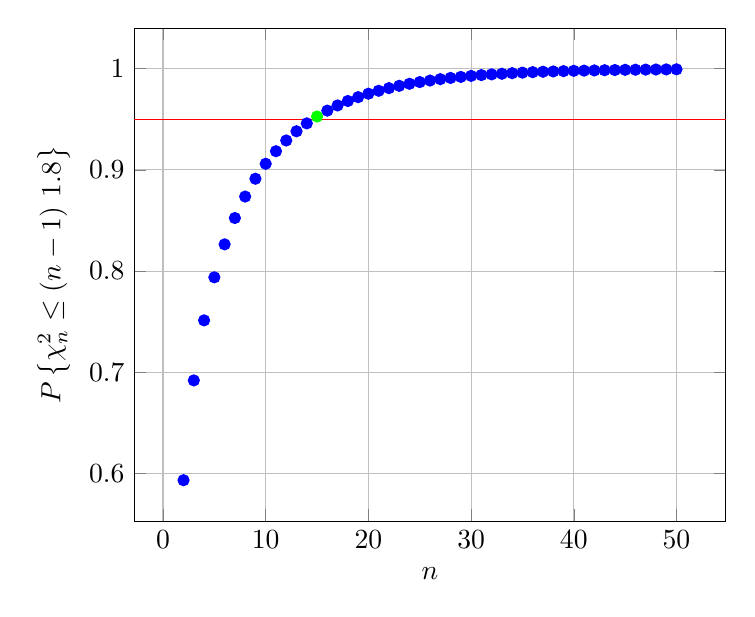
\begin{tikzpicture}
			\begin{axis}[width = 0.75\textwidth,xlabel=$n$, ylabel=$ P \left\{\chi_n^2 \leq (n-1)\ 1.8 \right\}  $, grid = both]
				
				\addplot[only marks, color = blue] plot coordinates{(2.0, 0.5934) (3.0, 0.692) (4.0, 0.7513) (5.0, 0.7938) (6.0, 0.8264) (7.0, 0.8524) (8.0, 0.8736) (9.0, 0.8912) (10.0, 0.906) (11.0, 0.9184) (12.0, 0.929) (13.0, 0.9381) (14.0, 0.9459) (16.0, 0.9585) (17.0, 0.9636) (18.0, 0.968) (19.0, 0.9718) (20.0, 0.9752) (21.0, 0.9781) (22.0, 0.9807) (23.0, 0.983) (24.0, 0.985) (25.0, 0.9867) (26.0, 0.9882) (27.0, 0.9896) (28.0, 0.9908) (29.0, 0.9918) (30.0, 0.9928) (31.0, 0.9936) (32.0, 0.9943) (33.0, 0.9949) (34.0, 0.9955) (35.0, 0.996) (36.0, 0.9965) (37.0, 0.9969) (38.0, 0.9972) (39.0, 0.9975) (40.0, 0.9978) (41.0, 0.998) (42.0, 0.9982) (43.0, 0.9984) (44.0, 0.9986) (45.0, 0.9988) (46.0, 0.9989) (47.0, 0.999) (48.0, 0.9991) (49.0, 0.9992) (50.0, 0.9993)};
				
				\addplot[only marks, color = green] plot coordinates{(15.0, 0.9527)};
				
				\draw [draw=red] (axis cs: -5,0.95) -- (axis cs: 60,0.95);
			\end{axis}
		\end{tikzpicture}
	\end{figure}
	
	\item Two samples with $ n_1 = 10, \sigma^2_1  = 4$ and $ n_2 = 5, \sigma^2_2  = 2$ \\
	
	
		\begin{align}
			\frac{S_1^2}{\sigma_1^2} &= \frac{\chi_9^2}{9} \qquad \frac{S_2^2}{\sigma_2^2} = \frac{\chi_4^2}{4} \nonumber \\
			%
			\frac{S_2^2}{S_1^2} &\geq 1 \qquad F_{4, 9} \geq 2 \nonumber \\
			%
			P  \left\{\frac{S_2^2}{S_1^2}  \geq 1\right\}  &= P \left\{F_{4, 9} \geq 2\right\}= 0.1782
		\end{align}
	
	
	\item $ n = 100, p  = 0.12$. Using the normal RV approximation with $ \mu = np = 12 $ and $ \sigma^2 = np(1-p)$ \\
	
	
		\begin{align}
			P \left\{9.5 \leq X \leq 14.5 \right\} &= P \left\{\frac{(9.5 - 12)}{\sqrt{12*0.88}} \leq Z \leq \frac{(14.5 - 12)}{\sqrt{12*0.88}} \right\} \nonumber \\
			%
			&= \Phi  \left(\frac{(14.5 - 12)}{\sqrt{12*0.88}}\right) - \Phi  \left(\frac{(9.5 - 12)}{\sqrt{12*0.88}}\right)  \nonumber \\
			%
			&= 0.5583
		\end{align}
	
	
	\item Each human is a binomial RV with $ p = 0.52 $. Let $ n $ vary and check probability including continuity correction\\
	
		\begin{align}
			P \left\{ X \geq 0.5n \right\} &= P \left\{ Z \geq \frac{0.5n - 0.52n - 0.5}{\sqrt{np(1-p)}} \right\} \\
			%
			n = 10 &\to P = 0.6711 \nonumber \\
			%
			n = 100 &\to P = 0.6916 \nonumber \\
			%
			n = 1000 &\to P = 0.9028 \nonumber \\
			%
			n = 10000 &\to P = 0.99997 \nonumber 
		\end{align}
	
	
	\item $ n = 300 $ men. $ c = 0.454, b = 0.284 $ \\
	
		\begin{enumerate}
			\item 			
			\begin{align}
				P \left\{X \geq 150 \right\} &= P \left\{Z \geq \frac{149.5 - 136.2}{\sqrt{300*0.454*0.546}} \right\} \nonumber \\
				%
				&= 0.0615
			\end{align}
			
			\item 
			\begin{align}
				P \left\{Y \leq 100 \right\} &= P \left\{Z \leq \frac{100.5 - 85.2}{\sqrt{300*0.284*0.716}} \right\} \nonumber \\
				%
				&= 0.9749
			\end{align}
			
		\end{enumerate}
	
	
	\item $ n = 300 $ women. $ d = 0.256, a = 0.214 $ \\
	
		\begin{enumerate}
			\item 			
			\begin{align}
				P \left\{V \geq 60 \right\} &= P \left\{Z \geq \frac{59.5 - 76.8}{\sqrt{300*0.256*0.744}} \right\} \nonumber \\
				%
				&= 0.9889
			\end{align}
			
			\item 
			\begin{align}
				P \left\{U \leq 50 \right\} &= P \left\{Z \leq \frac{50.5 - 64.2}{\sqrt{300*0.214*0.786}} \right\} \nonumber \\
				%
				&= 0.0269
			\end{align}
			
		\end{enumerate}
	
	
	\item More women than men rarely eat breakfast.
	$ \mathbb{E}[X-Y] = -10.2 $, and $\mathrm{Var}(X-Y) = 147.4452$\\
	
		\begin{align}
			P \left\{X > Y \right\} &= P \left\{ X - Y > 0 \right\} \nonumber \\
			%
			&= P \left\{ Z > \frac{0 + 10.2}{\sqrt{147.4452}}  \right\} = 0.2005
		\end{align}
	
	
	\item $ n = 1000 $ , $ p $ from the table as necessary.
	
		\begin{enumerate}
			\item 			
			\begin{align}
				P \left\{A \geq 500 \right\} &= P \left\{Z \geq \frac{500 - 542}{\sqrt{248.236}} \right\} \nonumber \\
				%
				&= 1 - \Phi \left( \frac{500 - 542}{\sqrt{248.236}} \right) = 0.9962
			\end{align}
			
			\item 
			\begin{align}
				P \left\{B > 500 \right\} &= P \left\{Z > \frac{500 - 704}{\sqrt{208.384}} \right\} \nonumber \\
				%
				&= 1 - \Phi \left( \frac{500 - 704}{\sqrt{208.384}} \right) \approx 1
			\end{align}
			
			\item 
			\begin{align}
				P \left\{C > 500 \right\} &= P \left\{Z > \frac{500 - 458}{\sqrt{248.236}} \right\} \nonumber \\
				%
				&= 1 - \Phi \left( \frac{500 - 458}{\sqrt{248.236}} \right) = 0.00384 \nonumber \\
				%
				P\left\{ \text{required} \right\} &= 0.00384 * 1 = 0.00384
			\end{align}
			
			\item 
			\begin{align}
				P \left\{D < 250 \right\} &= P \left\{Z < \frac{250 - 293}{\sqrt{207.151}} \right\} \nonumber \\
				%
				&= \Phi \left( \frac{250 - 293}{\sqrt{207.151}} \right) = 0.0014
			\end{align}
			
			\item 
			\begin{align}
				P \left\{E \geq 200 \right\} &= P \left\{Z \geq \frac{200 - 149}{\sqrt{126.799}} \right\} \nonumber \\
				%
				&= 1 - \Phi \left( \frac{200 - 149}{\sqrt{126.799}} \right) \approx 0
			\end{align}
			
			\item Let $ F = F_1 - F_2 $, with $ \mathbb{E}[F] = 31$, $ \mathrm{Var}[F] = 253.819$
			\begin{align}
				P \left\{F_1 - F_2 \geq 0 \right\} &= P \left\{Z \geq \frac{0 - 31}{\sqrt{253.819}} \right\} \nonumber \\
				%
				&= 1 - \Phi \left( \frac{0 - 31}{\sqrt{253.819}} \right) = 0.9742
			\end{align}
			
		\end{enumerate}
	
	
	\item Each worker belongs to a union where $ p = 0.105 $ with $ n = 5 $. The older value of $ q = 0.201 $\\
	$ \mathbb{E}[X-Y] = -10.2 $, and $\mathrm{Var}(X-Y) = 147.4452$\\
	
		\begin{align}
			P \left\{X = 0 \right\} &= (1-p)^5 = 0.5743 \\
			%
			P \left\{Y = 0 \right\} &= (1-q)^5 = 0.3256
		\end{align}
	
	
	\item $ n = 144 $ women. $ \mu = 517, \sigma = 120 $ \\
	
		\begin{enumerate}
			\item 			
			\begin{align}
				P \left\{\overline{X} > 507 \right\} &= P \left\{Z > \frac{507 - 517}{120/12} \right\} \nonumber \\
				%
				&= 1 - \Phi (-10/10) = 0.8413
			\end{align}
			
			\item 			
			\begin{align}
				P \left\{\overline{X} > 517 \right\} &= P \left\{Z > \frac{517 - 517}{120/12} \right\} \nonumber \\
				%
				&= 1 - \Phi (0/10) = 0.5
			\end{align}
			
			
			\item 			
			\begin{align}
				P \left\{\overline{X} > 537 \right\} &= P \left\{Z > \frac{537 - 517}{120/12} \right\} \nonumber \\
				%
				&= 1 - \Phi (20/10) = 0.0227
			\end{align}
			
			\item 			
			\begin{align}
				P \left\{\overline{X} > 550 \right\} &= P \left\{Z > \frac{550 - 517}{120/12} \right\} \nonumber \\
				%
				&= 1 - \Phi (33/10) = 0.00048
			\end{align}
			
		\end{enumerate}
	
	
	\item $ n = 12 $ women. $ \mu = 53600, \sigma = 3200 $ \\
	
	
		\begin{align}
			P \left\{\overline{X} > 55000 \right\} &= P \left\{Z > \frac{55000 - 53600}{3200/\sqrt{12}} \right\} \nonumber \\
			%
			&= 0.0648
		\end{align}
	
	
	\item $ n = $ is to be found. $ \mu = 100, \sigma = 30 $. Let $ Y = \sum X_i $ \\
	
	
		\begin{align}
			P \left\{Y > 2000 \right\} &= P \left\{Z > \frac{2000 - 100\ n}{30\ \sqrt{n}} \right\} \geq 0.95 \nonumber \\
			%
			\Phi \left( \frac{2000 - 100\ n}{30\ \sqrt{n}} \right) &\leq 0.05 \nonumber \\
			%
			2000 - 100\ n &\leq -1.6448 \times 30\sqrt{n} \nonumber \\
			%
			n &\geq 23
		\end{align}
		
		\begin{figure}[H]
			\centering
			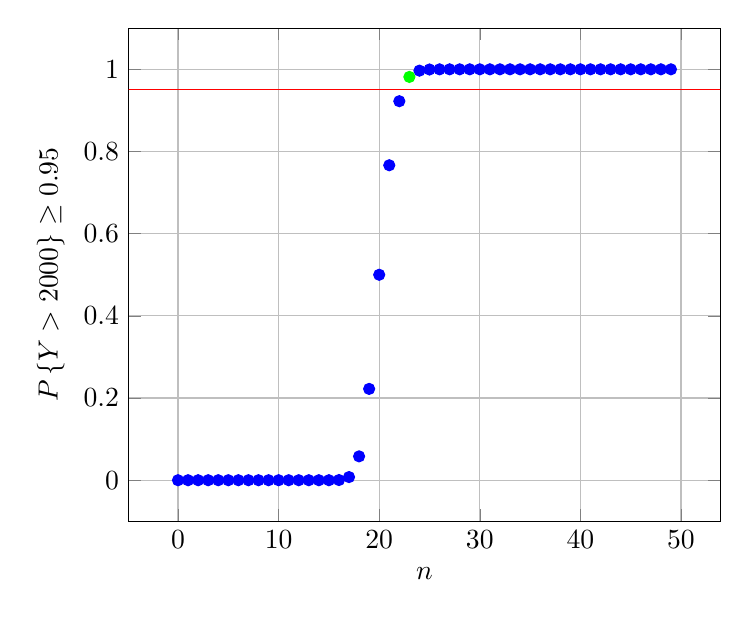
\begin{tikzpicture}
				\begin{axis}[width = 0.75\textwidth,xlabel=$n$, ylabel=$ P \left\{ Y > 2000 \right\} \geq 0.95  $, grid = both]
					
					\addplot[only marks, color = blue] plot coordinates{(0.0, 0.0) (1.0, 0.0) (2.0, 0.0) (3.0, 0.0) (4.0, 0.0) (5.0, 0.0) (6.0, 0.0) (7.0, 0.0) (8.0, 0.0) (9.0, 0.0) (10.0, 0.0) (11.0, 0.0) (12.0, 6.8833827526759706e-15) (13.0, 4.851663515381688e-11) (14.0, 4.5152443450824364e-08) (15.0, 8.413074170987578e-06) (16.0, 0.0004290603331967846) (17.0, 0.007646685515099505) (18.0, 0.058050871990274366) (19.0, 0.2222194112520176) (20.0, 0.5) (21.0, 0.7665073693266079) (22.0, 0.922390755157658) (24.0, 0.9967522068714105) (25.0, 0.9995709396668032) (26.0, 0.999956150288122) (27.0, 0.9999964472261701) (28.0, 0.9999997666572595) (29.0, 0.9999999873257626) (30.0, 0.9999999994204671) (31.0, 0.9999999999773364) (32.0, 0.9999999999992313) (33.0, 0.9999999999999771) (34.0, 0.9999999999999994) (35.0, 1.0) (36.0, 1.0) (37.0, 1.0) (38.0, 1.0) (39.0, 1.0) (40.0, 1.0) (41.0, 1.0) (42.0, 1.0) (43.0, 1.0) (44.0, 1.0) (45.0, 1.0) (46.0, 1.0) (47.0, 1.0) (48.0, 1.0) (49.0, 1.0)
					};
					
					\addplot[only marks, color = green] plot coordinates{(23.0, 0.9814718907179405)};
					
					\draw [draw=red] (axis cs: -5,0.95) -- (axis cs: 60,0.95);
				\end{axis}
			\end{tikzpicture}
		\end{figure}
	
\end{enumerate}
%	\chapter{Parameter Estimation}

\begin{enumerate}
	
	\item 
		To determine MLE of $ \theta $, first find the joint PDF $ f(x_1, x_2, \dots, x_n) $ \\
		\begin{align}
			f(x_1, x_2, \dots, x_n | \theta) &= \prod_{i=1}^{n} \exp(\theta-x_i) \qquad \forall\ x_i \geq \theta \nonumber \\
			%
			&= \exp \left[ \sum\limits_{i=1}^{n} (\theta - x_i) \right] = \exp \left[n\theta - \sum x_i\right] \nonumber \\
			%
			\log (f) &= n\theta - \sum x_i		
		\end{align} \\
		This is maximised when $ \theta $ is maximised, but $ \theta \leq x_i\ \forall i \in \{1,\dots, n\} $.\\
		Thus, $ \widehat{\theta} = \min(\{x_i\}) $ \\
	
	
	\item 
		\begin{align}
			f(x) &= 0.5\ \exp\left(-|x- \theta|\right) \qquad \forall\ x \in \mathbb{R} \nonumber \\
			%
			f(x_1, x_2, \dots, x_n | \theta) &= \frac{1}{2^n}\ \exp\left[ \sum\limits_{i=1}^{n} -|x_i - \theta| \right] \nonumber \\
			%
			\log (f) &= -n\log (2) - \sum\limits_{i=1}^{n} |x_i - \theta| 
		\end{align}
	 \\
	
	
	$ \sum |x_i - \theta| $ is total absolute error. This is minimized by $ \widehat{\theta} = \mathrm{median}(x_1, \dots, x_n)$\\
	
	\item $ \mu $ is known, find MLE of $ \sigma^2 $. To find joint PDF and thus likelihood function, \\
	
	
		\begin{align}
			f(x_1, x_2, \dots, x_n | \sigma^2) &= \left(\frac{1}{\sqrt{2\pi\sigma^2}}\right)^n\ \exp \left[\sum\limits_{i=1}^{n}\ \frac{-(x_i - \mu)^2}{2\sigma^2}\right] \nonumber \\
			%
			\log(f) &= -(n/2)\ \log(2\pi) - n\ \log(\sigma) - \left[\sum\limits_{i=1}^{n}\ \frac{(x_i - \mu)^2}{2\sigma^2}\right] \\
			%
			\frac{\mathrm{d}}{\mathrm{d} \sigma^2}\ \log(f) &= 0 \nonumber \\
			%
			0 &= -\ddfrac{n}{2\sigma^2} + \frac{\sum (x_i - \mu)^2}{2\sigma^4} \nonumber \\
			%
			\widehat{\sigma}^2 &= \frac{\sum (x_i - \mu)^2}{n} \\
			%
			\mathbb{E}\left[\widehat{\sigma^2}\right] &= 1/n \sum \mathbb{E}[(x_i - \mu)^2] = \sigma^2
		\end{align}\\
	
	\item Pareto density function with parameters $ (a, \lambda) $. Constraint on $ a $ is that $ a \leq \min({x_i}) $. \\
	Let $ y = \prod\limits_{i=1}^{n} x_i $
	
	
		\begin{align}
			f(x) &= \lambda a^\lambda x^{-(\lambda+1)} \qquad \forall\ x \geq a \nonumber \\
			%
			f(x_1, x_2, \dots, x_n | a, \lambda) &= \lambda^n\ a^{n\lambda}\ y^{-(\lambda + 1)} \\
			%
			\widehat{a} &= \min(\{x_i\}) \\
			%
			\frac{\mathrm{d}}{\mathrm{d} \lambda}\ (\log f) &= \frac{n}{\lambda} + n \log (a) - \log (y) \nonumber \\
			%
			\widehat{\lambda} &= \frac{n}{\log (y) - n \log (a)}
		\end{align}\\
	
	
	\item Given the three sets of RVs, with means $ \mu_1, \mu_2, (\mu_1 + \mu_2) $, and common variance $ \sigma^2 $. \\
	
	
		\begin{align}
			G_i(\mu_1, \mu_2) &= (x_i - \mu_1)^2 + (y_i - \mu_2)^2 + (w_i - \mu_1 - \mu_2)^2 \nonumber \\
			%
			f(x_1, y_1,w_1, \dots, x_n, y_n, w_n | \mu_1, \mu_2) &= \left(\frac{1}{\sqrt{2\pi\sigma^2}}\right)^{3n}\ \exp \left[-\sum\limits_{i=1}^{n}\ \frac{G_i(\mu_1, \mu_2)}{2\sigma^2}\right] \nonumber \\
			%
			\log(f) &= -(3n/2)\ \log(2\pi) - 3n\ \log(\sigma) \nonumber \\
			%
			&- \left[\sum\limits_{i=1}^{n}\ \frac{G_i(\mu_1, \mu_2)}{2\sigma^2}\right] \\
			%
			\frac{\mathrm{d}}{\mathrm{d} \mu_1}\ \log(f) &= 0 \nonumber \\
			%
			0 &= \frac{1}{\sigma^2}\ \sum\limits_{i=1}^{n}\ (x_i - \mu_1) + (w_i - \mu_1 - \mu_2) \nonumber \\
			%
			\overline{X} + \overline{W} &= (2\widehat{\mu_1} + \widehat{\mu_2}) \\
			%
			\overline{Y} + \overline{W} &= (\widehat{\mu_1} + 2\widehat{\mu_2}) \nonumber \\
			%
			\widehat{\mu_1} = \frac{2\overline{X} - \overline{Y} + \overline{W}}{3} \qquad &\text{and} \qquad \widehat{\mu_2} = \frac{-\overline{X} + 2\overline{Y} + \overline{W}}{3}
		\end{align} \\
	
	
	\item The sample mean and variance of $ Y = \log(X) $ is calculated as $ \overline{Y} = 3.7319,\ S_Y^2 = 0.0508 $. \\
	
	
		\begin{align}
			P \left\{ D \geq v \right\} &= 0.01 \nonumber \\
			%
			P \left\{ \frac{Y - \overline{Y}}{S_Y} \geq z_{0.01}\right\} &= 0.01 \nonumber \\
			%
			Y &\geq 9.8 \qquad \to \qquad X \geq 18041.35	
		\end{align}\\
	
	
	Thus, a 100-year flood has a discharge of $ 18041 $.
	
	\item $ X $ is a log-normal RV. Let $ Y = \log X $. The moment generating function leads to mean and variance.\\
	
		\begin{enumerate}
			\item Using the MGF of $ Y $, \\
			\begin{align}
				\phi_Y(t) &= \exp \left( \mu t  + \frac{\sigma^2 t^2}{2}\right) \nonumber \\
				%
				\mathbb{E}[e^{Yt}] &= \mathbb{E}[X^t] \nonumber \\
				%
				\mathbb{E}[X] &= \exp \left(\mu + \frac{\sigma^2}{2}\right)
			\end{align} \\
			
			\item To find variance, set $ t = 2 $, \\
			\begin{align}
				\mathbb{E}[X^2] &= \exp \left(2\mu + 2\sigma^2\right) \nonumber \\
				%
				\mathrm{Var}(X) &= \exp \left(2\mu + 2\sigma^2\right) - \exp \left(2\mu + \sigma^2\right)
			\end{align} \\
			
			\item Calculating mean travel time using the above formulae, \\
			find $\mu =  \overline{Y} = 45.4 $ and $ \sigma^2 = S_Y^2 = 131.82 $.\\
			
			\begin{align}
				\mathbb{E}[X] &= \exp \left(\mu + 0.5\sigma^2\right) = 45.56
			\end{align} \\
			
		\end{enumerate}
	
	
	\item The sample mean and variance of $ Y = X + \mathcal{N} (0, 0.1^2) $ is calculated as \\
	$ \overline{Y} = 3.1502,\ S_Y = 0.0092 $. \\
	
	
		\begin{align}
			Y &\sim \mathcal{N}(X, 0.1^2) \nonumber \\
			%
			\text{95\% confidence interval is } X &\in \left(\overline{Y} \pm\frac{\sigma\ z_{0.025}}{\sqrt{n}}\right) \nonumber \\
			%
			&= 3.1502 \pm 0.08765 = [3.0625, 3.2378] \\
			%
			\text{99\% confidence interval is } X &\in \left(\overline{Y} \pm\frac{\sigma\ z_{0.005}}{\sqrt{n}}\right) \nonumber \\
			%
			&= 3.1502 \pm 0.11519 = [3.0350, 3.2654]
		\end{align}\\
	
	
	\item The sample mean and variance of $ Y \sim \mathcal{N} (\mu, 0.08^2) $ is calculated as \\
	$ \overline{Y} = 11.48$. \\
	
	
		\begin{align}
			\text{95\% confidence interval is } \mu &\in \left(\overline{Y} \pm\frac{\sigma\ z_{0.025}}{\sqrt{n}}\right) \nonumber \\
			%
			&= 3.1502 \pm 0.04958 = [11.4304, 11.5296] \\
			%
			\text{95\% upper confidence interval is } X &\geq \overline{Y} - \frac{\sigma\ z_{0.05}}{\sqrt{n}} \nonumber \\
			%
			&= 3.1502 - 0.04161 = [11.4384, \infty) \nonumber \\
			%
			\text{95\% lower confidence interval is } X &\leq \overline{Y} + \frac{\sigma\ z_{0.05}}{\sqrt{n}} \nonumber \\
			%
			&= 3.1502 + 0.04161 = (-\infty, 11.5216]
		\end{align}\\
	
	
	\item The sample mean and variance of $ Y \sim \mathcal{N} (\mu, 11.3^2) $ is given as \\
	$ \overline{Y} = 74.6, n = 81$. \\
	
	
		\begin{align}
			\text{95\% confidence interval is } \mu &\in \left(\overline{Y} \pm \frac{\sigma\ z_{0.025}}{\sqrt{n}}\right) \nonumber \\
			%
			&= 74.6 \pm 2.0652 = [72.5348, 76.6652] 
		\end{align}\\
	
	
	\item $ \overline{X_n} $ is a the mean of the first $ n $ samples. $ \sigma^2 = 1 $ \\
	
		\begin{enumerate}
			\item Find the distribution of $ X_{n+1} - \overline{X}_n $, \\
			\begin{align}
				\overline{X_n} &\sim \mathcal{N}(\mu, \sigma^2/n) \nonumber \\
				%
				X_{n+1} &\sim \mathcal{N}(\mu, \sigma^2) \nonumber \\
				%
				X_{n+1} - \overline{X}_n &\sim \mathcal{N}(0,1 + 1/n)
			\end{align} \\
			
			\item $ \overline{X_n} = 4 $, \\
			\begin{align}
				\text{90\% confidence interval is } X_{n+1} &\in \left(\overline{X_n} \pm \sqrt{1 + 1/n}\ z_{0.05}\right)
			\end{align} \\
			
		\end{enumerate}
	
	
	\item The sample mean $ \mu $ is unknown and variance is known to be $ \sigma^2 $. For a $ 100(1-\alpha) $ lower confidence interval \\
	
	
		\begin{align}
			\frac{\overline{X} - \mu}{\sigma / \sqrt{n}} &\sim Z \nonumber \\
			%
			P \left\{\frac{\overline{X} - \mu}{\sigma / \sqrt{n}} > z_\alpha\right\} &= 1 - \alpha\\
			%
			\mu &< \overline{X} + \frac{z_\alpha\ \sigma}{\sqrt{n}} \nonumber \\
			%
			\mu &\in \left(-\infty\ ,\ \overline{X} + \frac{z_\alpha\ \sigma}{\sqrt{n}}\right]
		\end{align}\\
	
	
	\item The sample mean $ \mu $ is unknown and variance is known to be $ \sigma = 0.2 $. The 99\% two-sided confidence interval is \\
	$ \overline{Y} = 1.2, n = 20$. \\
	
		\begin{align}
			\mu &\in \left(\overline{Y} \pm \frac{\sigma\ z_{0.005}}{\sqrt{n}}\right) \nonumber \\
			%
			&= 1.2 \pm 0.1152 = [1.0848, 1.3152] 
		\end{align}\\
	
	
	\item Using problem 13 data but with $ \sigma $ unknown and $ S^2 = 0.04 $. For a 99\% confidence interval, use $ \alpha = 0.01 $, $ \overline{Y} = 1.2, n = 20$. \\
	
		\begin{align}
			\mu &\in \left[ \overline{Y} - \frac{(t_{\alpha/2, n-1})\ s}{\sqrt{n}}, \ \overline{Y} + \frac{(t_{\alpha/2, n-1})\ s}{\sqrt{n}} \right] \nonumber \\
			%
			\mu &\in 1.2 \pm 0.1279 = [1.0720, 1.3279]
		\end{align}\\
	
	
	\item Using problem 14 data to find one-sided 99\% confidence interval. \\
	
		\begin{align}
			\mu &\in \left(-\infty\ , \ \overline{Y} + \frac{(t_{\alpha, n-1})\ s}{\sqrt{n}} \right] \nonumber \\
			%
			c &= 1.2 + 0.1136 = 1.31357
		\end{align}\\
	
	
	\item First perform a sub-sampling with $ m = 30$ and use it to find the required sample size $ n $. Normal RV with both mean and variance unknown. \\
	
		\begin{enumerate}
			\item Using $ m = 30 $, this subsample has variance $ S^2_m $. The interval width will then be\\
			\begin{align}
				b = 2t_{\alpha/2, m-1}\ \frac{S_m}{\sqrt{m}}
			\end{align} \\
			
			\item For large $ n $, this can be approximated to a standard normal RV $ Z $. \\
			\begin{align}
				A = 2z_{\alpha/2}\ \frac{S_m}{\sqrt{n}}
			\end{align} \\
			Solving for $ n $ gives the size of the full sample. \\
		\end{enumerate}
	
	
	\item $ \sigma $ unknown and $ S = 6.9576 $. For a 95\% confidence interval, use $ \alpha = 0.01 $, $ \overline{Y} = 333.9958, n = 24$. Using a t-distribution with $ 23 $ DOF, which yields slightly larger intervals than a standard normal RV\\
	
		\begin{align}
			\mu &\in \left[ \overline{Y} - \frac{(t_{\alpha/2, n-1})\ s}{\sqrt{n}}, \ \overline{Y} + \frac{(t_{\alpha/2, n-1})\ s}{\sqrt{n}} \right] \nonumber \\
			%
			\mu &\in 333.9958 \pm 2.9379 = [331.0579, 336.9338] \qquad \text{95\% confidence} \nonumber \\
			%
			\mu &\in 333.9958 \pm 3.9870 = [330.0088, 337.9828] \qquad \text{99\% confidence} 
		\end{align}\\
	
	
	\item $ \sigma $ unknown and $ S = 10.2127 $, $ \overline{Y} = 133.22, n = 18$. Using a t-distribution with $ 17 $ DOF, which yields slightly larger intervals than a standard normal RV\\
	
		\begin{align}
			\mu &\in \left[ \overline{Y} - \frac{(t_{\alpha/2, n-1})\ s}{\sqrt{n}}, \ \overline{Y} + \frac{(t_{\alpha/2, n-1})\ s}{\sqrt{n}} \right] \nonumber \\
			%
			\mu &\in 333.9958 \pm 4.3125 = [128.9097, 137.5347] \qquad \text{95\% confidence} \nonumber \\
			%
			\mu &\in \left(-\infty\ ,\  137.5312\right] \qquad \text{lower 95\% confidence} \nonumber \\
			%
			\mu &\in \left[128.9133\ ,\ \infty\right) \qquad \text{upper 95\% confidence}
		\end{align}\\
	
	
	\item $ \sigma $ unknown and $ S = 22 $, $ \overline{Y} = 222, n = 9$. Using a t-distribution with $ 8 $ DOF, which yields slightly larger intervals than a standard normal RV\\
	
		\begin{align}
			\mu &\in \left[ \overline{Y} - \frac{(t_{\alpha, n-1})\ s}{\sqrt{n}}, \infty \right) \nonumber \\
			%
			\mu &\in \left[208.363\ ,\ \infty\right) \qquad \text{upper 95\% confidence}
		\end{align}\\
	
	
	\item $ \sigma $ unknown and $ S = 800 $, $ \overline{Y} = 2200, n = 18$. Using a t-distribution with $ 15 $ DOF, which yields slightly larger intervals than a standard normal RV\\
	
		\begin{align}
			\mu &\in \left[ \overline{Y} - \frac{(t_{\alpha/2, n-1})\ s}{\sqrt{n}}, \ \overline{Y} + \frac{(t_{\alpha/2, n-1})\ s}{\sqrt{n}} \right] \nonumber \\
			%
			\mu &\in 333.9958 \pm 350.61 = [1849.3899, 2550.6101] \qquad \text{90\% confidence}
		\end{align}\\
	
	
	\item $ \sigma $ unknown and $ S = 16 $, $ \overline{Y} = 320, n = 100$. Using a t-distribution with $ 99 $ DOF, which yields slightly larger intervals than a standard normal RV\\
	
		\begin{align}
			\mu &\in \left[ \overline{Y} - \frac{(t_{\alpha/2, n-1})\ s}{\sqrt{n}}, \ \overline{Y} + \frac{(t_{\alpha/2, n-1})\ s}{\sqrt{n}} \right] \nonumber \\
			%
			\mu &\in 320 \pm 3.1747 = [316.8252, 323.1747] \qquad \text{95\% confidence}
		\end{align}\\
	
	
	\item $ \sigma $ unknown and $ S = 15.4 $, $ \overline{Y} = 330.2, n = 20$. Using a t-distribution with $ 19 $ DOF, which yields slightly larger intervals than a standard normal RV\\
	
		\begin{align}
			\mu &\in \left[ \overline{Y} - \frac{(t_{\alpha/2, n-1})\ s}{\sqrt{n}}, \ \overline{Y} + \frac{(t_{\alpha/2, n-1})\ s}{\sqrt{n}} \right] \nonumber \\
			%
			\mu &\in 330.2 \pm 7.2074 = [322.9926, 337.4074] \qquad \text{95\% confidence} \nonumber \\
			%
			\mu &\in 330.2 \pm 9.8517 = [320.3482, 340.0517] \qquad \text{99\% confidence}
		\end{align}\\
	
	
	\item $ \sigma $ unknown and $ S = 840 $, $ \overline{Y} = 1220, n = 300$. Using a t-distribution with $ 299 $ DOF, which yields slightly larger intervals than a standard normal RV\\
	
		\begin{align}
			\mu &\in \left[ \overline{Y} - \frac{(t_{\alpha/2, n-1})\ s}{\sqrt{n}}, \ \overline{Y} + \frac{(t_{\alpha/2, n-1})\ s}{\sqrt{n}} \right] \nonumber \\
			%
			\mu &\in 1220 \pm 95.4395 = [1124.5605, 1315.4395] \qquad \text{95\% confidence} 
		\end{align}\\
	
	
	\item from Problem 23,\\
	
		\begin{align}
			\mu &\in \left(-\infty\ ,\  \overline{Y} - \frac{(t_{\alpha, n-1})\ s}{\sqrt{n}} \right] \nonumber \\
			%
			\mu &\in \left(-\infty\ ,\ 1282.2896  \right] \qquad \text{upper 90\% confidence} \nonumber \\
			%
			v &= 1282.2896
		\end{align}\\
	
	
	\item confidence interval for $ \mu $ when $ \sigma^2 $ is unknown. Using the sample mean and sample variance $ \overline{X}, S^2 $, and the observations for these statistics $ \overline{x}, s^2 $\\
	
		\begin{align}
			\frac{\overline{X} - \mu}{S/\sqrt{n}} &\sim t_{n-1} \nonumber \\
			%
			P \left\{ \frac{\overline{X} - \mu}{S/\sqrt{n}} > -t_{\alpha, n-1}\right\} &= 1 - \alpha \nonumber \\
			%
			\mu \in \left( -\infty\ ,\ \overline{x} + \frac{t_{\alpha, n-1}\ s}{\sqrt{n}} \right]
		\end{align}\\
	
	
	\item $ \sigma $ unknown and $ S = 104.3435 $, $ \overline{Y} = 2062.75, n = 20$. Using a t-distribution with $ 19 $ DOF, which yields slightly larger intervals than a standard normal RV\\
	
		\begin{align}
			\mu &\in \left[ \overline{Y} - \frac{(t_{\alpha/2, n-1})\ s}{\sqrt{n}}, \ \overline{Y} + \frac{(t_{\alpha/2, n-1})\ s}{\sqrt{n}} \right] \nonumber \\
			%
			\mu &\in 2062.75 \pm 48.8343 = [2013.9157, 2111.5843] \qquad \text{95\% confidence} \nonumber \\
			%
			\mu &\in 2062.75 \pm 66.7511 = [1995.9989, 2129.5011] \qquad \text{99\% confidence} \nonumber \\
			%
			v &= 2022.41
		\end{align}\\
	
	
	\item $ \sigma $ unknown and $ S = 8.6879 $, $ \overline{Y} = 98.67, n = 20$. Using a t-distribution with $ 19 $ DOF, which yields slightly larger intervals than a standard normal RV\\
	
		\begin{align}
			\mu &\in \left[ \overline{Y} - \frac{(t_{\alpha/2, n-1})\ s}{\sqrt{n}}, \ \overline{Y} + \frac{(t_{\alpha/2, n-1})\ s}{\sqrt{n}} \right] \nonumber \\
			%
			\mu &\in 98.67 \pm 4.0660 = [94.6039, 102.7360] \qquad \text{95\% confidence} 
		\end{align}\\
	
	
	\item $ \sigma $ unknown and $ S = 0.02944 $, $ \overline{Y} = 0.55, n = 10$. Using a t-distribution with $ 9 $ DOF, which yields slightly larger intervals than a standard normal RV\\
	
		\begin{align}
			\mu &\in \left[ \overline{Y} - \frac{(t_{\alpha/2, n-1})\ s}{\sqrt{n}}, \ \overline{Y} + \frac{(t_{\alpha/2, n-1})\ s}{\sqrt{n}} \right] \nonumber \\
			%
			\mu &\in 0.55 \pm 0.02106 = [0.52894, 0.57106] \qquad \text{95\% confidence} 
		\end{align}\\
	
	
	\item 
		To find the PMF of $ N $, look at the CDF of $ N $ first. $ \mathbb{E}[U_i] = 1/2, \mathrm{Var}(U_i) = 1/12 $\\
		Consider $ S_n = U_1 + \dots + U_n $ and some. This is the $ n $ dimensional simplex problem.\\
		
		When finding the area of the $ n $-simplex, 
		
		Begin by proving the recursion formula for the volume of an $ n $ dimensional simplex. Let $ {X_i} $ be such that uniform RV $ X_i \in [0, 1] $ and the constraint $ \sum x_i  \leq 1$. \\
		
		Using analytical methods to find the exact asymptotic value of $ \mathbb{E}[X] $
		\begin{align}
			P\{S_1 \leq 1\} = A_1 &= P\{X_1 \leq 1\} = 1 \nonumber \\
			%
			P\{S_2 \leq 1\} = A_2 &= \int\limits_{0}^{1} \int\limits_{0}^{1-y} \mathrm{d}x\ \mathrm{d}y = \frac{1}{2}\\
			%
			P\{S_3 \leq 1\} = A_3 &= \int\limits_{0}^{1} (1-z)^2\ A_2\ \mathrm{d}z = \frac{A_2}{3} = \frac{1}{6}\\
			%
			P\{S_n \leq 1\} = A_n &= \int_{0}^{1} (1-x_n)^{n-1}\ A_{n-1}\ \mathrm{d}x_n = \frac{A_{n-1}}{n}		
		\end{align}\\
		
		The above factor of $ (1-x_n)^{n-1} $ arises as a result of all of the other $ n-1 $ dimensions being scaled down by a factor of $ 1-x_n $ when $ x_n > 0 $. From recursion, $ A_n = 1/n!$\\
		
		Now, using the above as a CDF of $ N $, then its PDF and expected value\\
		\begin{align}
			P\{N \leq n\} &= 1 - P\{N > n\} = A_n = 1 - \frac{1}{n!} \nonumber \\
			%
			P\{N = n\} &= P\{N \leq n\} - P\{N \leq n-1\} = \frac{n-1}{n!} \\
			%
			\mathbb{E}[X] &= \sum\limits_{i=1}^{\infty} i\ P\{N = i\} = \sum\limits_{i=0}^{\infty} \frac{1}{i!} = e 
		\end{align}
		
		
		Thus, the expected value of $ X $ converges to the natural logarithm $ e $.\\
		
		Using a Monte-Carlo simulation with $ n = k^2 \ \forall\ k \in [4, 99]$ \\
		
		\begin{figure}[H]
			\centering
			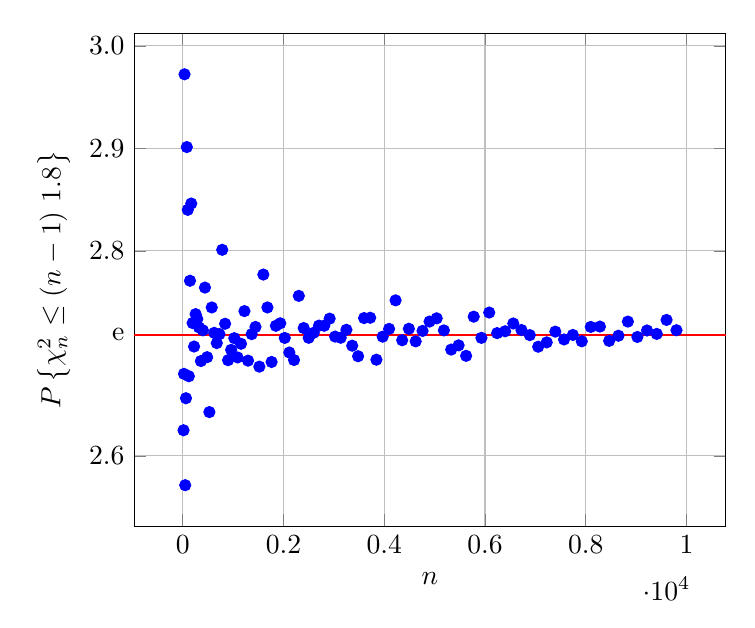
\begin{tikzpicture}
				\begin{axis}[width = 0.75\textwidth,xlabel=$n$, ylabel=$ P \left\{\chi_n^2 \leq (n-1)\ 1.8 \right\}  $, grid = both, ytick = {2.4, 2.6, e, 2.8, 2.9, 3.0}, yticklabels = {2.4, 2.6, e, 2.8, 2.9, 3.0}]
					
					\addplot[only marks, color = blue] plot coordinates{(16, 2.625) (25, 2.68) (36, 2.9722222222222223) (49, 2.5714285714285716) (64, 2.65625) (81, 2.9012345679012346) (100, 2.84) (121, 2.677685950413223) (144, 2.7708333333333335) (169, 2.8461538461538463) (196, 2.729591836734694) (225, 2.7066666666666666) (256, 2.73828125) (289, 2.7335640138408306) (324, 2.7253086419753085) (361, 2.6925207756232687) (400, 2.7225) (441, 2.764172335600907) (484, 2.696280991735537) (529, 2.6427221172022684) (576, 2.7447916666666665) (625, 2.72) (676, 2.710059171597633) (729, 2.718792866941015) (784, 2.8010204081632653) (841, 2.728894173602854) (900, 2.6933333333333334) (961, 2.7034339229968785) (1024, 2.71484375) (1089, 2.6960514233241506) (1156, 2.709342560553633) (1225, 2.7412244897959184) (1296, 2.692901234567901) (1369, 2.718772826880935) (1444, 2.7257617728531858) (1521, 2.6870479947403023) (1600, 2.776875) (1681, 2.744794765020821) (1764, 2.691609977324263) (1849, 2.7268793942671716) (1936, 2.729338842975207) (2025, 2.7150617283950615) (2116, 2.700850661625709) (2209, 2.6935264825712992) (2304, 2.756076388888889) (2401, 2.724698042482299) (2500, 2.7152) (2601, 2.7201076509034987) (2704, 2.7270710059171597) (2809, 2.7269490922036312) (2916, 2.7338820301783264) (3025, 2.7163636363636363) (3136, 2.7152423469387754) (3249, 2.7229916897506925) (3364, 2.7074910820451845) (3481, 2.697213444412525) (3600, 2.7344444444444442) (3721, 2.734748723461435) (3844, 2.693808532778356) (3969, 2.7163013353489545) (4096, 2.723876953125) (4225, 2.751715976331361) (4356, 2.7128099173553717) (4489, 2.7239919803965247) (4624, 2.7117214532871974) (4761, 2.7219071623608486) (4900, 2.7310204081632654) (5041, 2.734179726244793) (5184, 2.72241512345679) (5329, 2.70369675361231) (5476, 2.70781592403214) (5625, 2.6976) (5776, 2.735803324099723) (5929, 2.7151290268173387) (6084, 2.7398093359631823) (6241, 2.7197564492869732) (6400, 2.7215625) (6561, 2.7291571406797743) (6724, 2.7227840571088637) (6889, 2.717811003048338) (7056, 2.7064909297052155) (7225, 2.710726643598616) (7396, 2.721200648999459) (7569, 2.7135685031047694) (7744, 2.71797520661157) (7921, 2.711778815806085) (8100, 2.7258024691358025) (8281, 2.7261200338123417) (8464, 2.7121928166351608) (8649, 2.717192739044976) (8836, 2.730986871887732) (9025, 2.71601108033241) (9216, 2.7223307291666665) (9409, 2.7189924540333723) (9604, 2.7326114119117033) (9801, 2.722579328639935)};
					
					\draw [thick, draw=red,] (axis cs: -1000, e ) -- (axis cs: 11000,  e );
				\end{axis}
			\end{tikzpicture}
		\end{figure}
	
	
	\item $ \sigma $ unknown and $ S = 3.9799 $, $ \overline{Y} = 11.5666, n = 30$. Using a t-distribution with $ 29 $ DOF, which yields slightly larger intervals than a standard normal RV\\
	
		\begin{align}
			\mu &\in \left[ \overline{Y} - \frac{(t_{\alpha/2, n-1})\ s}{\sqrt{n}}, \ \overline{Y} + \frac{(t_{\alpha/2, n-1})\ s}{\sqrt{n}} \right] \nonumber \\
			%
			\mu &\in 11.5666 \pm 1.4861 = [10.0805, 13.0528] \qquad \text{95\% confidence} 
		\end{align}\\
	
	
	\item $ \sigma $ unknown and $ S = 9400 $, $ \overline{Y} = 90450, n = 16$. Using a t-distribution with $ 15 $ DOF, which yields slightly larger intervals than a standard normal RV\\
	
		\begin{align}
			\mu &\in \left[ \overline{Y} - \frac{(t_{\alpha/2, n-1})\ s}{\sqrt{n}}, \ \overline{Y} + \frac{(t_{\alpha/2, n-1})\ s}{\sqrt{n}} \right] \nonumber \\
			%
			\mu &\in 90450 \pm 5008.9064 = [85441.0936, 95458.9064] \qquad \text{95\% confidence} 
		\end{align}\\
	
	
	\item Find the mean squared error of the predictor $ \overline{X} $, \\
	
		\begin{align}
			\overline{X_n} &\sim \mathcal{N}(\mu, \sigma^2/n) \nonumber \\
			%
			X_{n+1} &\sim \mathcal{N}(\mu, \sigma^2) \nonumber \\
			%
			Y = X_{n+1} - \overline{X_n} &\sim \mathcal{N}(0, \sigma^2\ (1+1/n))\nonumber \\
			%
			\mathbb{E}[Y^2] &= \mathrm{Var}(Y) + \left(\mathbb{E}[Y]\right)^2 = \sigma^2\ \left(1+\frac{1}{n}\right)
		\end{align}\\
	
	
	\item $ \sigma $ unknown and $ S = 0.3775 $, $ \overline{Y} = 4.725, n = 4$. Using a t-distribution with $ 3 $ DOF, which yields slightly larger intervals than a standard normal RV\\
	
		\begin{align}
			\frac{X_{n+1} - \overline{X}_n}{S_n \sqrt{1 + 1/n}} &\sim t_{n-1} \nonumber \\
			%
			\mu &\in \left[ \overline{Y} - (t_{\alpha/2, n-1})\ s \sqrt{1 + 1/n}, \ \overline{Y} + (t_{\alpha/2, n-1})\ s \sqrt{1 + 1/n} \right] \nonumber \\
			%
			\mu &\in 4.725 \pm 1.3431 = [3.3818, 6.0681] \qquad \text{95\% confidence} 
		\end{align}\\
	
	
	\item  $ \sigma $ unknown and $ S = 2.12 $, $ \overline{Y} = 2.5, n = 30$. Using a t-distribution with $ 29 $ DOF, which yields slightly larger intervals than a standard normal RV,\\
	
		\begin{align}
			\mu &\in \left(-\infty\ ,\  \overline{Y} - \frac{(t_{\alpha, n-1})\ s}{\sqrt{n}} \right] \nonumber \\
			%
			\mu &\in \left(-\infty\ ,\ 3.0076  \right] \qquad \text{upper 90\% confidence} \nonumber \\
			%
			v &= 3.0076
		\end{align}\\
	
	
	\item  Verifying the one-sided confidence intervals for $ \sigma^2 $ when the mean is unknown,\\
	
		\begin{align}
			\frac{(n-1)S^2}{\sigma^2} &\sim \chi^2_{n-1} \nonumber \\
			%
			P \left\{ \frac{(n-1)S^2}{\sigma^2} \leq \chi^2_{\alpha, n-1} \right\} &= 1 - \alpha \nonumber \\
			%
			\sigma^2 &\in \left[ \frac{(n-1)S^2}{\chi^2_{\alpha, n-1}}\ ,\ \infty \right) \\
			%
			P \left\{ \frac{(n-1)S^2}{\sigma^2} \geq \chi^2_{1 - \alpha, n-1} \right\} &= 1 - \alpha \nonumber \\
			%
			\sigma^2 &\in \left(0\ ,\ \frac{(n-1)S^2}{\chi^2_{1-\alpha, n-1}} \right]
		\end{align}\\
	
	
	\item  $ \sigma $ unknown and $ S^2 = 32.2333 $, $ \overline{Y} = 144.3, n = 10$. Using a t-distribution with $ 9 $ DOF, which yields slightly larger intervals than a standard normal RV,\\
	
		\begin{align}
			\sigma^2 &\in \left[\frac{(n-1)S^2}{\chi^2_{\alpha/2, n-1}} ,\  \frac{(n-1)S^2}{\chi^2_{1 -\alpha/2, n-1}} \right] \nonumber \\
			%
			\sigma^2 &\in \left[ 12.2979, 167.2111 \right] \qquad \text{95\% confidence} \nonumber \\
			%
			v &= 69.6 \qquad \text{using upper 90\% confidence}
		\end{align}\\
	
	
	\item  $ \sigma $ unknown and $ S^2 = 0.00313 $, $ \overline{Y} = 6.7236, n = 36$. Using a chi-squared distribution with $ 35 $ DOF, which yields slightly larger intervals than a standard normal RV,\\
	
		\begin{align}
			\sigma^2 &\in \left[\frac{(n-1)S^2}{\chi^2_{\alpha/2, n-1}} ,\  \frac{(n-1)S^2}{\chi^2_{1 -\alpha/2, n-1}} \right] \nonumber \\
			%
			\sigma^2 &\in \left[ 0.00206, 0.00532 \right] \qquad \text{95\% confidence} 
		\end{align}\\
	
	
	\item  $ \sigma $ unknown but equal. Using $ S_1^2 = 2.5\ ,\ S_2^2 = 7\ , n = 5\ , m = 3 $\\
	
		\begin{align}
			S_P^2 &= \frac{(n-1)\ S_1^2 + (m-1)\ S_2^2}{(n+m-2)} \nonumber \\
			%
			&= 4
		\end{align}\\
	
	
	\item  $ \mu = 3.180 $ but unknown $ \sigma $. Using the sample variance, $ S = 0.008 \approx \sigma $\\
	Using a chi-squared distribution with $ 7 $ DOF, which yields slightly larger intervals than a standard normal RV,\\
	
	
		\begin{align}
			\sigma &\in [0.0057, 0.0145]
		\end{align}\\
	
	
	\item  $ \mu $ is known. Using the sample variance, $ S = 0.008 \approx \sigma $\\
	Using a chi-squared distribution with $ 7 $ DOF, which yields slightly larger intervals than a standard normal RV,\\
	
	
		\begin{align}
			\mu &= \sum X_i / n \nonumber \\
			%
			S^2 &= \ddfrac{\sum (X_i - \overline{X})^2}{n-1} \nonumber \\
			%
			\text{estimator } \widehat{S^2} &= \ddfrac{\sum (X_i - \mu)^2}{n} \\
			%
			\frac{(n-1)S^2}{\sigma^2} \to \frac{n\widehat{S^2}}{\sigma^2} &\implies \chi^2_{n-1} \to \chi^2_{n}
		\end{align}\\
	
	
	Now, $ n \widehat{S^2} /\sigma^2 $ is a chi-squared distribution with $ n $ DOF. One extra DOF from knowledge of the population mean, acts like one extra observation.\\
	
	What burning time?\\
	
	\item  $ \sigma $ unknown but equal and $ \overline{X} - \overline{Y} = 227.7 $, pooled estimator of variance $ S_P = 266.6, n = m = 10$. \\
	Using a t distribution with $ 18 $ DOF, which yields slightly larger intervals than a standard normal RV,\\
	
		\begin{align}
			\mu_1 - \mu_2 &\in \left[ \overline{x} - \overline{y} - t_{\alpha / 2, n+m-2}\ s_p\ \sqrt{\frac{1}{n} + \frac{1}{m}}\ ,\ \overline{x} - \overline{y} + t_{\alpha / 2, n+m-2}\ s_p\ \sqrt{\frac{1}{n} + \frac{1}{m}} \right]  \nonumber \\
			%			
			\mu_1 - \mu_2 &\in 227.7 \pm 250.4841 = [-22.7841, 478.1841] \qquad \text{95\% confidence}  \nonumber \\
			%
			\mu_1 - \mu_2 &\in  [20.9549, \infty) \qquad \text{upper 95\% confidence} \nonumber \\
			%
			\mu_1 - \mu_2 &\in  (-\infty, 434.4451] \qquad \text{lower 95\% confidence} \nonumber 
		\end{align}\\
	
	
	\item  $ \sigma $ unknown but equal and $ \overline{X} - \overline{Y} = -10 $, pooled estimator of variance $ S_P = , n = 36, m = 64$. \\
	Using a t distribution with $ 18 $ DOF, which yields slightly larger intervals than a standard normal RV,\\
	
		\begin{align}
			\mu_1 - \mu_2 &\in \left[ \overline{x} - \overline{y} - t_{\alpha / 2, n+m-2}\ s_p\ \sqrt{\frac{1}{n} + \frac{1}{m}}\ ,\ \overline{x} - \overline{y} + t_{\alpha / 2, n+m-2}\ s_p\ \sqrt{\frac{1}{n} + \frac{1}{m}} \right]  \nonumber \\
			%			
			\mu_1 - \mu_2 &\in -10 \pm 1.179 = [-11.179, -8.821] \qquad \text{99\% confidence}  
		\end{align}\\
	
	
	\item  $ \sigma_1 = 4, \sigma_2 = 5 $ are known  $ \overline{X} - \overline{Y} = -10 $, pooled estimator of variance is no longer used. $n = 36, m = 64$ \\
	Using a standard normal distribution since population variances are known,\\
	
		\begin{align}
			\mu_1 - \mu_2 &\in \left[ \overline{x} - \overline{y} - z_{\alpha / 2} \sqrt{\frac{\sigma_1^2}{n} + \frac{\sigma_2^2}{m}}\ ,\ \overline{x} - \overline{y} + z_{\alpha / 2} \sqrt{\frac{\sigma_1^2}{n} + \frac{\sigma_2^2}{m}} \right]   \nonumber \\
			%			
			\mu_1 - \mu_2 &\in -10 \pm 1.12 = [-11.12, -8.88] \qquad \text{99\% confidence}  
		\end{align}\\
	
	
	
	\item  $ \sigma $ unknown but equal and $ \overline{X} - \overline{Y} = -16.5 $, pooled estimator of variance $ S_P = 45.411, n = m = 10$. \\
	
	Using a t distribution with $ 18 $ DOF, which yields slightly larger intervals than a standard normal RV,\\
	
		\begin{align}		
			\mu_1 - \mu_2 &\in -16.5 \pm 58.4569 = [-74.9569, 41.9569] \qquad \text{99\% confidence}
		\end{align}\\
	
	
	\item  $ \sigma_1^2, \sigma_2^2 $ unknown and $ \mu_1, \mu_2 $ known. $ \{X_i\}, \{Y_j\} $ are two sets of independent normal RV samples drawn from these two distributions. \\
	
	
		\begin{align}		
			\text{estimator } \widehat{S^2} &= \ddfrac{\sum (X_i - \mu)^2}{n} \nonumber \\
			%
			\frac{(n-1)S^2}{\sigma^2} \to \frac{n\widehat{S^2}}{\sigma^2} &\implies \chi^2_{n-1} \to \chi^2_{n} \nonumber \\
			%
			\sigma_1^2 &= \frac{\widehat{S_1^2}}{\chi_n^2/n} \qquad \text{and} \qquad \sigma_2^2 = \frac{\widehat{S_2^2}}{\chi_m^2/m} \\
			%
			\frac{\sigma_1^2}{\sigma_2^2}\ \frac{\widehat{S_2^2}}{\widehat{S_1^2}} &= \ddfrac{\chi_m^2/m}{\chi_n^2/n} \sim F_{m, n} \\
			%
			\frac{\sigma_1^2}{\sigma_2^2} &\in \left[ \frac{\widehat{S_1^2}}{\widehat{S_2^2}}\ F_{1 - \alpha/2, m, n}\ ,\ \frac{\widehat{S_1^2}}{\widehat{S_2^2}}\ F_{\alpha/2, m, n} \right]
		\end{align}\\
		
		The above F-distribution has parameters $ (m, n) $ instead of $ (m-1, n-1) $ as a result of the mean values being known. Refer problem 40 above for the explanation.\\
	
	
	\item  $ \sigma_1^2, \sigma_2^2 $ unknown and $ \mu_1, \mu_2 $ also unknown. $ \{X_i\}, \{Y_j\} $ are two sets of independent normal RV samples drawn from these two distributions. \\
	
	
		\begin{align}		
			\text{estimator } S^2 &= \ddfrac{\sum (X_i - \overline{X})^2}{n-1} \nonumber \\
			%
			\frac{\sigma_1^2}{\sigma_2^2}\ \frac{S_2^2}{S_1^2} &= \ddfrac{\chi_{m-1}^2/(m-1)}{\chi_{n-1}^2/(n-1)} \sim F_{m-1, n-1} \\
			%
			\frac{\sigma_1^2}{\sigma_2^2} &\in \left[0.02867, 0.58046\right] \qquad \text{95\% confidence}
		\end{align}\\
	
	
	\item Bernoulli RV using given data to estimate $ \widehat{p} $, and use it to find a confidence interval for $ p $ \\
	
		\begin{enumerate}
			\item $ \widehat{p}  = 0.3958$ \\
			\begin{align}
				p &\in \left[ \widehat{p} - z_{\alpha/2}\sqrt{\frac{\widehat{p}(1-\widehat{p})}{n}}\ ,\ \widehat{p} + z_{\alpha/2}\sqrt{\frac{\widehat{p}(1-\widehat{p})}{n}}  \right] \nonumber \\
				%
				p &\in 0.3958 \pm 0.0231 = [0.3728, 0.4189] \qquad \text{95\% confidence}
			\end{align} \\
			
			\item $ \widehat{p}  = 0.3897$ \\
			\begin{align}
				p &\in 0.3897 \pm 0.03729 = [0.3523, 0.4269] \qquad \text{95\% confidence}
			\end{align} \\
		\end{enumerate}
	
	
	\item Bernoulli RV using given data to estimate $ \widehat{p} $, and use it to find a confidence interval for $ p $ \\
	
		\begin{enumerate}
			\item $ \widehat{p}  = 0.17$ \\
			\begin{align}
				p &\in \left[ \widehat{p} - z_{\alpha/2}\sqrt{\frac{\widehat{p}(1-\widehat{p})}{n}}\ ,\ \widehat{p} + z_{\alpha/2}\sqrt{\frac{\widehat{p}(1-\widehat{p})}{n}}  \right] \nonumber \\
				%
				p &\in 0.17 \pm 0.01783 = [0.1522, 0.1878] \qquad \text{95\% confidence}
			\end{align} \\
			
			\item $ \widehat{p}  = 0.1067$ \\
			\begin{align}
				p &\in 0.1067 \pm 0.01466 = [0.092, 0.1213] \qquad \text{90\% confidence}
			\end{align} \\
		\end{enumerate}
	
	
	\item Bernoulli RV using given data to estimate $ \widehat{p} $, and use it to find a confidence interval for $ p $ \\
	
		\begin{enumerate}
			\item $ \widehat{p}  = 0.5106$ \\
			\begin{align}
				p &\in \left[ \widehat{p} - z_{\alpha/2}\sqrt{\frac{\widehat{p}(1-\widehat{p})}{n}}\ ,\ \widehat{p} + z_{\alpha/2}\sqrt{\frac{\widehat{p}(1-\widehat{p})}{n}}  \right] \nonumber \\
				%
				p &\in 0.5106 \pm 0.00822 = [0.5024, 0.5188] \qquad \text{90\% confidence}
			\end{align} \\
			
			\item $ \widehat{p}  = 0.5106$ \\
			\begin{align}
				p &\in 0.5106 \pm 0.0098 = [0.5008, 0.5204] \qquad \text{95\% confidence}
			\end{align} \\
		\end{enumerate}
	
	
	\item  Airline needs the width of the $ 90\% $ confidence interval to be 2\% of the parameter value. Using the maximum value of $ \widehat{p}\ (1-\widehat{p}) = 1/4 $ in order to find the minimum bound on $ n $\\
	
	
		\begin{align}		
			p &\in \left[ \widehat{p} - z_{\alpha/2}\sqrt{\frac{\widehat{p}(1-\widehat{p})}{n}}\ ,\ \widehat{p} + z_{\alpha/2}\sqrt{\frac{\widehat{p}(1-\widehat{p})}{n}}  \right] \nonumber \\
			%
			z_{\alpha/2}\sqrt{\frac{\widehat{p}(1-\widehat{p})}{n}} &= 0.02 \nonumber \\
			%
			n &= \frac{z_{0.05}^2\ \widehat{p}\ (1-\widehat{p})}{(0.02)^2} \qquad \text{rounded up to integer} \nonumber \\
			%
			n &\geq 4147 \qquad \text{to guarantee interval size}
		\end{align}\\
	
	
	\item No, since the intervals for the respective candidates $ [49, 57]\% $ and $ [43, 51]\% $ have some overlap.\\
	
	\item Same as Problem 50, $ n \geq 4147 $ to be $ 90\% $ confident that the result is within $ 2\% $ of the true value. \\
	
	\item $ \widehat{p}  = 79/140, n = 140$. To find the maximum error of the estimate, \\
	
		\begin{align}
			\text{Error } &= z_{0.01/2}\sqrt{\frac{\widehat{p}(1-\widehat{p})}{n}} \nonumber \\
			%
			&= 0.1079
		\end{align}
	
	
	\item $ \widehat{p}  = 0.17, n = 100$. Assume each item is independently defective with the same probability, \\
	
		\begin{align}
			p &\in \left[ \widehat{p} - z_{\alpha/2}\sqrt{\frac{\widehat{p}(1-\widehat{p})}{n}}\ ,\ \widehat{p} + z_{\alpha/2}\sqrt{\frac{\widehat{p}(1-\widehat{p})}{n}}  \right] \nonumber \\
			%
			p &\in 0.17 \pm 0.0736 = [0.0964, 0.2436] \qquad \text{95\% confidence} \\
			%
			p &\in \left[0.0826\ ,\ \infty \right) \qquad \text{upper 99\% confidence} 
		\end{align}\\
	
	
	\item $ \widehat{p}  = 0.67, n = 100$. Assume each person is independently likely to die in 5 years with the same probability, \\
	
		\begin{align}
			\text{Error } &= z_{0.05/2}\sqrt{\frac{\widehat{p}(1-\widehat{p})}{n}} \leq 0.02 \nonumber \\
			%
			n &\geq 2401 \to \text{additional samples required}\ =\ 2301
		\end{align}\\
	
	
	\item $ n $ independent Bernoulli RVs with parameter $ p $. \\
	
	
		\begin{align}
			p &\in \left[ \widehat{p} - z_{\alpha/2}\sqrt{\frac{\widehat{p}(1-\widehat{p})}{n}}\ ,\ \widehat{p} + z_{\alpha/2}\sqrt{\frac{\widehat{p}(1-\widehat{p})}{n}}  \right] \\
			%
			p &\in \left( -\infty\ ,\ \widehat{p} + z_{\alpha}\sqrt{\frac{\widehat{p}(1-\widehat{p})}{n}}  \right] \qquad \text{lower confidence}\\
			%
			p &\in \left[ \widehat{p} - z_{\alpha/2}\sqrt{\frac{\widehat{p}(1-\widehat{p})}{n}}\ ,\ \infty  \right) \qquad \text{upper confidence}
		\end{align}\\
	
	
	\item $ \widehat{\theta}  = 36, n = 10$. Each battery's lifetime is an exponential RV with mean $ \theta $, \\
	
		\begin{align}
			\theta &\in \left[\ddfrac{2 \sum X_i}{\chi^2_{\alpha/2, 2n}}\ ,\ \ddfrac{2 \sum X_i}{\chi^2_{1 - \alpha/2, 2n}}\right] \nonumber \\
			%
			\theta &\in [21.07, 75.07]
		\end{align}\\
	
	
	\item $ \widehat{\theta}  = 36, n = 10$. Each battery's lifetime is an exponential RV with mean $ \theta $, \\
	
		\begin{align}
			\theta &\in \left(-\infty\ ,\ \ddfrac{2 \sum X_i}{\chi^2_{1 - \alpha, 2n}}\right] \nonumber \\
			%
			\theta &\in (-\infty, 66.65] \\
			%
			\theta &\in \left[\ddfrac{2 \sum X_i}{\chi^2_{\alpha, 2n}}\ ,\ \infty \right) \nonumber \\
			%
			\theta &\in [22.92, \infty)
		\end{align}\\
	
	
	\item Unknown mean value $ \theta $ of an exponential RV from which $ n $ samples are drawn, find the unbiased estimator with the minimal mean squared error. Since the estimator is unbiased, this is equal to its variance. \\
	Since $ X_i \ \forall\ i \in \{1, n\}$ are unbiased estimators themselves, with $ \mathbb{E}[X_i] = \theta $ and $ \mathrm{Var}(X_i) = \sigma^2 $ 
	
		\begin{align}
			d(\theta) &= \sum \lambda_i\ X_i \qquad \text{such that} \qquad \sum \lambda_i = 1 \\
			%
			\widehat{\lambda_i} &= \ddfrac{1/\sigma^2_i}{\sum 1/\sigma_i^2} 
		\end{align}\\
		is the choice of $ \lambda $ that minimizes mean squared error. This reduces to $ \lambda_i = 1/n $ when all of the estimators have the same variance.\\
	
	
	\item Since $ X_i \ \forall\ i \in \{1, n\}$ are unbiased estimators themselves, with $ \mathbb{E}[X_i] = \theta $ and $ \mathrm{Var}(X_i) = \sigma^2 $ \\
	
		\begin{align}
			(n-1)S_x^2 / \sigma^2 \sim \chi_{n-1}^2 \qquad &\text{and} \qquad (m-1)S_y^2 / \sigma^2 \sim \chi_{m-1}^2 \nonumber \\
			%
			\mathrm{Var}(S_x^2) = \ddfrac{2\sigma^4}{(n-1)} \qquad &\text{and} \qquad \mathrm{Var}(S_y^2) = \ddfrac{2\sigma^4}{(m-1)} \nonumber \\
			%
			\lambda_1 = \ddfrac{1/\mathrm{Var}(S_x^2)}{1/\mathrm{Var}(S_x^2) + 1/\mathrm{Var}(S_y^2)} &= \frac{n-1}{n+m-2} \\
			%
			\lambda_2 = \ddfrac{1/\mathrm{Var}(S_y^2)}{1/\mathrm{Var}(S_x^2) + 1/\mathrm{Var}(S_y^2)} &= \frac{m-1}{n+m-2}
		\end{align}\\
		This proves the pooled estimator results stated above.\\
	
	
	\item  $ \mathbb{E}[d_1] = \theta, \mathrm{Var}(d_1) = 6 $ while $ \mathbb{E}[d_2] = 2 + \theta, \mathrm{Var}(d_2) = 2 $. Comparing the mean squared errors of these estimators,\\
	
		\begin{align}
			r(d_i, \theta) &= \mathrm{Var}(d_i) + b_\theta^2 (d_i) \nonumber \\
			%
			r(d_1, \theta) &= 6 + 0^2 = 6 \qquad \text{while} \qquad r(d_2, \theta) = 2 + 2^2 = 6
		\end{align}\\
		Both estimators have the same mean squared error, but only one of them is unbiased. They are equally good. \\
	
	
	\item Accidents $ Y $ is a Poisson RV with unknown $ \lambda $. A prior for $ \lambda $ is assumed and the Bayes estimator is then found. \\
	
		\begin{align}
			p(\lambda) &= e^{-\lambda} \qquad \forall\ \lambda > 0 \nonumber \\
			%
			f(\lambda\ |\ x) &= \ddfrac{f(x\ |\ \lambda)\ p(\lambda)}{\int f(x\ |\ \lambda)\ p(\lambda)\ \mathrm{d}\lambda} \\
			%
			\text{numerator}&= e^{-\lambda}\ \left[e^{-10\lambda}\ \dfrac{(10\lambda)^{83}}{83!}\right] \nonumber \\
			%
			\text{denominator}&= \int\limits_{\lambda=0}^{\infty} e^{-\lambda}\ \left[e^{-10\lambda}\ \dfrac{(10\lambda)^{83}}{83!}\ \mathrm{d}\lambda\right] \nonumber \\
			%
			&= \int\limits_{\lambda=0}^{\infty} e^{-a\lambda}\ \lambda^{b}\ \mathrm{d}\lambda = \frac{\Gamma(b+1)}{a^{b+1}}\nonumber \\
			%
			f(\lambda\ |\ x) &= \frac{a\ e^{-a\lambda}\ (a\lambda)^{b}}{\Gamma(b+1)} \sim \Gamma(b+1, a) \\
			%
			\mathbb{E}[f(\lambda\ |\ x)] &= (b+1/a) = 84/11 = 7.64
		\end{align}\\
		
		The MLE of the mean of a Poisson distribution is simply the population mean which is $ 8.3 $.
	
	
	\item Lifetime $ Y $ is an exponential RV with unknown $ \lambda $. A prior for $ \lambda $ is assumed and the Bayes estimator is then found. Let $ z = 1 + \sum x_i $\\
	
		\begin{align}
			p(\lambda) &= e^{-\lambda} \frac{\lambda^2}{2!}\qquad \forall\ \lambda > 0 \nonumber \\
			%
			f(\theta\ |\ x_1, \dots, x_n) &= \ddfrac{f(x_1, \dots, x_n\ |\ \theta)\ p(\theta)}{\int\limits f(x_1, \dots, x_n\ |\ \theta)\ p(\theta)\  \mathrm{d}\theta} \\
			%
			\text{numerator}&= \lambda e^{-4.6\lambda }\ \left[e^{-\lambda}\ \dfrac{(\lambda)^{2}}{2!}\right] \nonumber \\
			%
			\text{denominator}&= \int\limits_{\lambda=0}^{\infty} \lambda^{n+2}\ e^{-\lambda z}\ \mathrm{d}\lambda \nonumber \\
			%
			&= \frac{\Gamma(n+3)}{z^{n+3}}\nonumber \\
			%
			f(\lambda\ |\ x) &= \frac{\lambda z\ e^{-\lambda z}\ (\lambda z)^{n+2}}{\Gamma(n+3)} \sim \Gamma(n+3, z) \\
			%
			\mathbb{E}[f(\lambda\ |\ x)] &= (23/93) = 0.2473
		\end{align}\\
	
	
	\item $ Y $ is a Bernoulli RV with unknown $ p $. A prior for $ \lambda $ is assumed and the Bayes estimator is then found. Let $ r $ be defective out of 10 chosen.\\
	
		\begin{align}
			p(\lambda) &= 1\qquad \forall\ \lambda \in [0, 1] \nonumber \\
			%
			f(\theta\ |\ x_1, \dots, x_n) &= \ddfrac{f(x_1, \dots, x_n\ |\ \theta)\ p(\theta)}{\int\limits f(x_1, \dots, x_n\ |\ \theta)\ p(\theta)\  \mathrm{d}\theta} \\
			%
			\text{numerator}&= \binom{10}{r}\ p^r\ (1-p)^{10-r} \nonumber \\
			%
			\text{denominator}&= \int\limits_{p=0}^{1} \binom{10}{r}\ p^r\ (1-p)^{10-r}\ \mathrm{d}p \nonumber \\
			%
			&= \frac{\Gamma(r+1)\ \Gamma(11-r)}{\Gamma(12)}\nonumber \\
			%
			f(\lambda\ |\ x) &= \frac{11!\ p^r\ (1-p)^{10-r}}{r!\ (10-r)!}
			%
		\end{align}\\
		Integration is not possible analytically. So, numerical integration will yield the value of the estimator for different $ r $ values. \\
	
	
	\item Using the given values of $ \sigma_0 = 3, \mu = 200, \sigma = 2, \overline{X} = 182, n = 20 $
	
		\begin{align}
			\mathbb{E}[\theta\ |\ X_1, \dots, X_n] &= \left(\frac{n\sigma^2}{n\sigma^2 + \sigma_0^2}\right)\ \overline{X} + \left(\frac{\sigma_0^2}{n\sigma^2 + \sigma_0^2}\right)\ \mu \nonumber \\
			%
			&= 183.82 \nonumber \\
			%
			\mathrm{Var}(\theta\ |\ X_1, \dots, X_n) &= \frac{\sigma^2 \sigma_0^2}{n\sigma^2 + \sigma_0^2} = 0.4045 \nonumber \\
			%
			\theta &\in 183.82 \pm 1.246 = [182.5737, 185.0667]
		\end{align}
	
	
	
	
\end{enumerate}
%	\chapter{Hypothesis Testing}


\begin{flushright}
	\textit{``\dots beyond a reasonable doubt."} 
\end{flushright}

In addition to the problem of estimating the unknown parameters of an underlying distribution from which samples are drawn, it is also useful to test some assertions about the sample itself.

\textbf{Hypothesis} : A statement about the parameters of the underlying distribution from which a sample has been drawn. Direct information about these parameters is most often unavailable. A hypothesis is \textit{accepted} if a random sample from the population is consistent with the assertion made.

Statistical tests to \textit{accept} a hypothesis do not conclude that it is true. They merely conclude that the sample used to test it is consistent with the hypothesis. In other words, a hypothesis, if true, might have reasonably led to the sample having the observed values.


\textbf{Significance levels} : Consider a distribution $ F_\theta $ where $ \theta $ is an unknown parameter. In order to test some hypothesis about $ \theta $, it is useful to define a \textit{null hypothesis} $ H_0 $. A null hypothesis is \textit{simple} or \textit{composite}, depending on whether or not it completely specifies the probability distribution when true.

\textit{Critical region} : When a sample $ \{X_i\} $ of size $ n $ is drawn to test a null hypothesis, the condition for rejecting it is for the sample to lie in some region of $ n -$dimensional space $ C \in \mathbb{R}^n $, called the critical region.

\textit{Errors in testing a hypothesis} : The two possible types of errors when testing a hypothesis are the false rejection (\textit{Type I}) and the false acceptance (\textit{Type II}). Depending on the real-world application, one of these types of errors might be considered a much bigger issue than the other.

\textit{Level of significance} : Define a scalar $ \alpha $, such that whenever $ H_0 $ is true, the probability of being rejected is never greater than $ \alpha $. This is called the significance level of the test. Conventional values of $ \alpha = 0.1, 0.05, 0.005 $ are common in science literature.

\begin{align}
	P  \left\{\text{Type I error}\right\} \leq \alpha 
\end{align}

The general procedure to develop a null hypothesis is as follows

\begin{itemize}
	\item Determine a point estimator $ d(\textbf{X}) $ of the parameter $ \theta $.
	\item Find the probability distribution of $ d(\textbf{X}) $ provided $ H_0 $ is true.
	\item Determine the critical region correspoding to the required level of significance $ \alpha $.
	\item For a null hypothesis which asserts that the parameter $ \theta $ lies in some region $ w $,
	 $ H_0 : \theta \in w $ is rejected if $ d(\textbf{X}) $ lies in the critical region $ C $ or equivalently is 'far away' from $ w $.
\end{itemize}


\textbf{Tests - Mean of a normal RV} : A normal RV is extremely common in many real-world applications which makes the problem of testing hypotheses about its mean value very important, with strategies differing based on knowledge of its variance.

\textit{Known Variance} : Using the usual sample notation, consider the null hypothesis $ H_0 : \mu = \mu_0 $ proposed against the alternative hypothesis $ H_1 : \mu \neq \mu_0 $. Here $ \mu_0 $ is some assumed constant.

Rearranging the sample mean $ \overline{X} $, which is the point estimator of $ \mu $, to yield a standard normal distribution gives the critical region and thus the hypothesis rejection condition.
\begin{align}
	P_{\mu_0} \left\{ \Big|\overline{X} - \mu_0\Big|  > c\right\} &= \alpha \\
	%
	\frac{\overline{X} - \mu_0}{\sigma / \sqrt{n}} &\sim Z \nonumber \\
	%
	P \left\{Z > z_{\alpha/2}\right\} &= \alpha/2 \nonumber \\
	%
	\text{reject $ H_0 $ if } \qquad & \frac{\sqrt{n}}{\sigma}\ \Big| \overline{X} - \mu_0 \Big| > z_{\alpha/2} \nonumber \\
	%
	\text{accept $ H_0 $ if } \qquad & \frac{\sqrt{n}}{\sigma}\ \Big| \overline{X} - \mu_0 \Big| \leq z_{\alpha/2}
\end{align}

The above notation $ P_{\mu_0} $ denotes the probability given that $ \mu = \mu_0 $.

\textit{p-value} : The probability that a standard normal in absolute value $ |Z| $ will exceed the quantity above on the LHS, is called the p-value of a test.
\begin{align}
	P \left\{ |Z| > \frac{\sqrt{n}}{\sigma} \Big| \overline{X} - \mu_0 \Big| \right\} &= p \nonumber \\
	%
	\text{reject $ H_0 $ if } \qquad & p \leq \alpha \nonumber \\
	%
	\text{accept $ H_0 $ if } \qquad & p > \alpha	
\end{align}

\textit{Power function of a test} : In order to measure the probability of a type-II error, define the \textit{Operating Characteristic} (OC) curve $ \beta(\mu) $ as,

\begin{align}
	\beta(\mu) &= P_{\mu} \left\{\text{acceptance of $ H_0 $}\right\} \\
	%
	&= P_{\mu} \left\{ Z \in \frac{\mu_0 - \mu}{\sigma/\sqrt{n}} \pm z_{\alpha/2} \right\} \nonumber \\
	%
	&= \Phi\left(\frac{\mu_0 - \mu}{\sigma/\sqrt{n}} + z_{\alpha/2}\right) - \Phi\left( \frac{\mu_0 - \mu}{\sigma/\sqrt{n}} - z_{\alpha/2} \right)
\end{align}

The probability of rejection when $ \mu $ is the true value is $ 1 - \beta(\mu) $. This is called the power-function of the test.

Using the power-function, the probability of hypothesis acceptance when the true mean is $ \mu_1 $ is expressed as $ \beta(\mu_1) \approx \beta $. The sample size $ n $ needed to ensure this is calculated as

\begin{align}
	\beta &= \Phi\left(\frac{\mu_0 - \mu_1}{\sigma/\sqrt{n}} + z_{\alpha/2}\right) - \Phi\left( \frac{\mu_0 - \mu_1}{\sigma/\sqrt{n}} - z_{\alpha/2} \right) \nonumber \\
	%
	&\approx \Phi\left(\frac{\mu_0 - \mu_1}{\sigma/\sqrt{n}} + z_{\alpha/2}\right) = P\left\{Z > z_\beta\right\}\nonumber
\end{align}

The second term above is considered so small as to be close to zero and thus ignored.

\begin{align}
	\Phi(-z_\beta) &= \Phi\left(\frac{\mu_0 - \mu_1}{\sigma/\sqrt{n}} + z_{\alpha/2}\right) \nonumber \\
	%
	n &\approx \frac{\sigma^2\ (z_{\alpha/2} + z_\beta)^2}{(\mu_1 - \mu_0)^2}
\end{align}

\textit{One-sided tests} : Using the same reasoning as the two-sided tests above, the two possible kinds of one-sided testing problem are defined as

\begin{align}
	H_0 : \mu = \mu_0 \qquad &\text{vs.} \qquad H_1 : \mu > \mu_0 \nonumber \\
	%
	H_0 : \mu \leq \mu_0 \qquad &\text{vs.} \qquad H_1 : \mu > \mu_0 \nonumber \\
	%	
	\text{reject $ H_0 $ if } \qquad & \frac{\sqrt{n}}{\sigma}\ (\overline{X} - \mu_0)  > z_{\alpha} \nonumber \\
	%
	\text{accept $ H_0 $ if } \qquad & \frac{\sqrt{n}}{\sigma}\  (\overline{X} - \mu_0)  \leq z_{\alpha}
\end{align}

This leads to the corresponding power function and OC curve being a decreasing function of $ \mu $. In the above one-sided tests, a reversal of the inequalities reverses the sign of $ z_\alpha $

\begin{align}
	\beta(\mu) &= \Phi\left(\frac{\mu_0 - \mu}{\sigma/\sqrt{n}} + z_{\alpha}\right) \\
	%
	\beta(\mu_0) &= 1 - \alpha
\end{align}

\begin{align}
	H_0 : \mu = \mu_0 \qquad &\text{vs.} \qquad H_1 : \mu < \mu_0 \nonumber \\
	%
	H_0 : \mu \geq \mu_0 \qquad &\text{vs.} \qquad H_1 : \mu < \mu_0  \nonumber \\
	%	
	\text{reject $ H_0 $ if } \qquad & \frac{\sqrt{n}}{\sigma}\ (\overline{X} - \mu_0)  < -z_{\alpha} \nonumber \\
	%
	\text{accept $ H_0 $ if } \qquad & \frac{\sqrt{n}}{\sigma}\  (\overline{X} - \mu_0)  \geq -z_{\alpha}
\end{align}

A test is robust if it functions well even when the underlying assumptions enabling the test are violated. The Central Limit theorem is often the root cause of such robustness.

Notice the direct similarity between the calculation of $ 100(1-\alpha)\% $ confidence intervals and the $ \alpha $-level significance test. The probability distributions used to justify both of these procedures are the exact same.

\textit{Unknown Variance (the t-test) } : The much more common real-world case of a normal distribution with both mean and variance unknown requires the t-distribution to enable significance tests. Using the sample variance $ S^2 $ to estimate the population variance $ \sigma^2 $,

\begin{align}
	\frac{\overline{X} - \mu_0}{S / \sqrt{n}} &\sim t_{n-1} \nonumber \\
	%
	P \left\{ -t_{\alpha/2, n-1} \leq \frac{\overline{X} - \mu_0}{S / \sqrt{n}} \leq t_{\alpha/2, n-1} \right\} &= 1- \alpha \nonumber \\
	%
	H_0 : \mu = \mu_0 \qquad &\text{vs.} \qquad H_1 : \mu \neq \mu_0 \nonumber \\
	%
	\text{reject $ H_0 $ if } \qquad & \frac{\sqrt{n}}{S}\ \Big| \overline{X} - \mu_0 \Big| > t_{\alpha/2, n-1} \nonumber \\
	%
	\text{accept $ H_0 $ if } \qquad & \frac{\sqrt{n}}{S}\ \Big| \overline{X} - \mu_0 \Big| \leq t_{\alpha/2, n-1}
\end{align}

The corresponding one-sided t-tests also resemble the one-sided z-tests outlined above, with the only changes being the replacement of $ \sigma $ with $ S $ and the distribution changing from $ z_\alpha $ to $ t_{\alpha, n-1} $.

\textbf{Equality of means of two normal populations} : To test if the means $ \mu_x $ and $ \mu_y $ of two normal RVs with variances $ \sigma_x^2 $ and $ \sigma_y^2 $ which may or may not be known, samples of size $ n, m $ are drawn and the difference of sample means $ \overline{X} - \overline{Y} $ is rearranged to create standard probability distributions.

The real-world problem requiring this procedure is the testing of whether or not two different approaches to solving the same problem yield similar-enough results.

\textit{Known variances} : Following the earlier z-test defined above,

\begin{align}
	\overline{X} - \overline{Y} &\sim \mathcal{N}\left( \mu_x - \mu_y, \frac{\sigma_x^2}{n} + \frac{\sigma_y^2}{m} \right) \nonumber \\
	%
	H_0 : \mu_x = \mu_y \qquad &\text{vs.} \qquad H_1 : \mu_x \neq \mu_y \nonumber \\
	%
	\text{reject $ H_0 $ if } \qquad & \ddfrac{| \overline{X} - \overline{Y} |}{\sqrt{\sigma_x^2/n + \sigma_y^2/m}} > z_{\alpha/2}  \nonumber \\
	%
	\text{accept $ H_0 $ if } \qquad & \ddfrac{| \overline{X} - \overline{Y} |}{\sqrt{\sigma_x^2/n + \sigma_y^2/m}} \leq z_{\alpha/2}
\end{align}

The one-sided test results are not repeated here as they are similar to earlier results above.

\textit{Unknown but equal variances} : Using the sample variances $ S_x^2, S_y^2 $ to calculate the pooled estimator $ S_P^2 $, the difference between the sample means can be reanrranged into a t-RV with $ n+m-2 $ DOF.

Assuming the unknown variances are equal, $ \sigma_x^2 = \sigma_y^2 = \sigma^2$,

\begin{align}
	S_P^2 &= \frac{(n-1)\ S_1^2 + (m-1)\ S_2^2}{(n+m-2)} \nonumber \\
	%
	\ddfrac{\overline{X} - \overline{Y} - (\mu_x - \mu_y)}{\sqrt{S_P^2(1/n + 1/m)}} &\sim t_{n+m-2} \nonumber \\
	%	
	H_0 : \mu_x = \mu_y \qquad &\text{vs.} \qquad H_1 : \mu_x \neq \mu_y  \nonumber\\
	%
	\text{reject $ H_0 $ if } \qquad & \ddfrac{| \overline{X} - \overline{Y} |}{\sqrt{S_P^2(1/n + 1/m)}} > t_{\alpha/2, n+m-2}  \nonumber \\
	%
	\text{accept $ H_0 $ if } \qquad & \ddfrac{| \overline{X} - \overline{Y} |}{\sqrt{S_P^2(1/n + 1/m)}} \leq t_{\alpha/2, n+m-2}
\end{align}

The one-sided tests are not stated here as they are similar to the earlier one-sided t-tests above.

\textit{Unknown and unequal variances} : The exact formulation of an $ \alpha $-level significance test when the variances are unknown and unequal is not a solved problem. However, under the assumption of very large sample sizes $ n, m $, an approximately standard normal test can be constructed as

\begin{align}
	\overline{X} - \overline{Y} &\approx \mathcal{N}\left( \mu_x - \mu_y, \frac{S_x^2}{n} + \frac{S_y^2}{m} \right) \nonumber \\
	%
	H_0 : \mu_x = \mu_y \qquad &\text{vs.} \qquad H_1 : \mu_x \neq \mu_y \nonumber \\
	%
	\text{reject $ H_0 $ if } \qquad & \ddfrac{| \overline{X} - \overline{Y} |}{\sqrt{S_x^2/n + S_y^2/m}} > z_{\alpha/2} \nonumber \\
	%
	\text{accept $ H_0 $ if } \qquad & \ddfrac{| \overline{X} - \overline{Y} |}{\sqrt{S_x^2/n + S_y^2/m}} \leq z_{\alpha/2}
\end{align}

\textit{paired t-test} : Consider the real-world case where each of the $ n $ items are not independent. The problem of measuring the change in each element of the set after some action cannot be done using the above procedures because of the lack of independence.

If $ \{X_n\} $ and $ \{Y_n\} $ are the set of observations for each of the $ n $ objects before and after an experiment, then a new variable $ W_i = X_i - Y_i $ can still be used to perform significance tests on the effects of this experiment.

\begin{align}
	\frac{\overline{W} - \mu_w}{S_w / \sqrt{n}} &\sim t_{n-1} \nonumber \\
	%
	H_0 : \mu_w = 0 \qquad &\text{vs.} \qquad H_1 : \mu_w \neq 0 \nonumber \\
	%
	\text{reject $ H_0 $ if } \qquad & \frac{\sqrt{n}}{S_w}\ \Big| \overline{W} \Big| > t_{\alpha/2, n-1} \nonumber \\
	%
	\text{accept $ H_0 $ if } \qquad & \frac{\sqrt{n}}{S_w}\ \Big| \overline{W} \Big| \leq t_{\alpha/2, n-1}
\end{align}

The paired t-test is powerful in terms of not requiring independence of the $ n $ samples or knowledge of the variances $ \sigma_x^2, \sigma_y^2 $. A similar one-sided test can be constructed imitating earlier t-tests and is not stated here.

\textbf{Tests - Variance of a normal RV} : Given an underlying normal RV with unknown parameters $ (\mu, \sigma^2) $, hypothesis testing on the variance exploits the fact that for some specific value $ \sigma_0 $,

\begin{align}
	(n-1)\ \frac{S^2}{\sigma_0^2} &\sim \chi^2_{n-1} \nonumber \\
	%
	H_0 : \sigma^2 = \sigma_0^2 \qquad &\text{vs.} \qquad H_1 : \sigma^2 \neq \sigma_0^2 \\
	%
	\text{accept $ H_0 $ if } \qquad & (n-1)\ \frac{S^2}{\sigma_0^2} \in \left[ \chi^2_{1 - \alpha/2, n-1}\ ,\ \chi^2_{\alpha/2, n-1} \right] \\
	%
	\text{reject $ H_0 $} \qquad & \text{otherwise}
\end{align}

\textbf{Equality of variances of two normal populations} : Using the sample variances $ S_x^2, S_y^2 $ for two samples with $ n, m $ elements and rearranging them into an F-distribution,

\begin{align}
	\frac{S^2_x}{S^2_y} &\sim F_{n-1, m-1} \nonumber \\
	%
	H_0 : \sigma_x^2 = \sigma_y^2 \qquad &\text{vs.} \qquad H_1 : \sigma_x^2 \neq \sigma_y^2 \nonumber \\
	%
	\text{accept $ H_0 $ if } \qquad & \frac{S^2_x}{S^2_y} \in \left[ F_{1 - \alpha/2, n-1, m-1}\ ,\ F_{\alpha/2, n-1, m-1} \right] \nonumber \\
	%
	\text{reject $ H_0 $} \qquad & \text{otherwise}
\end{align}

\textbf{Tests - Bernoulli populations} : Since the Bernoulli RV is a discrete RV, it is treated differently from the continuous RV approaches above. For a Bernoulli RV with parameters $ (n, p) $, a one-sided significance test is constructed for a specific value $ p_0 $ as follows,

\begin{align}
	H_0 : p  \leq p_0 \qquad &\text{vs.} \qquad H_1 : p  > p_0 \\
	%
	P \{X \geq k\} &\leq \sum\limits_{i=k}^{n} \binom{n}{i}\ p_0^i\ (1-p_0)^{n-i}
\end{align}

The above relation holds true when $ H_0 $ is true and $ p \leq p_0 $. Now, the null hypothesis will be rejected when the number of samples possessing the property of interest $ X $, is larger than some threshold $ k^* $

\begin{align}
	\text{reject $ H_0 $ if } \qquad & X \geq k^*  \nonumber \\
	%
	k^* &= \min \left\{k\ :\ \sum\limits_{i=k}^{n} \binom{n}{i}\ p_0^i\ (1-p_0)^{n-i} \leq \alpha \right\} \nonumber \\
	%
	\text{accept $ H_0 $} \qquad & \text{otherwise}
\end{align}

The normal approximation to the Bernoulli RV when $ n $ is large and $ p $ is small also enables the use of the z-test on the transformed variable as outlined above.

\begin{align}
	\frac{X - np_0}{\sqrt{np_0(1-p_0)}} &\sim Z \nonumber
\end{align}

The corresponding two sided significance test involves rejection of the null hypothesis if $ X $ is either much larger or much smaller than the expected value of the Binomial RV with $ p = p_0 $, and observed value of the RV $ X = x $,

\begin{align}
	H_0 : p  = p_0 \qquad &\text{vs.} \qquad H_1 : p  \neq p_0 \nonumber \\
	%
	\text{reject $ H_0 $ if } \qquad & P\{\texttt{binom}(n, p_0) \geq x\} \leq \alpha/2  \nonumber \\
	%
	\text{or }& P\{\texttt{binom}(n, p_0) \leq x\} \leq \alpha/2 \nonumber \\
	%
	\text{accept $ H_0 $} \qquad & \text{otherwise}
\end{align}

\textbf{Equality of parameters in two Bernoulli RVs} : Consider two samples of size $ n, m $ each with elements that independently have a probability $ p, q $ of having a desired property.

Let $ X, Y $ be binomial RVs measuring the number of desirable elements from each population. They have Bernoulli parameters $ (n,p) $ and $ (m, q) $ respectively. Let $ k = X + Y $ be the total number of desirable elements from the combined sample pool $ n+m $.

\begin{align}
	H_0 : p  = q \qquad &\text{vs.} \qquad H_1 : p  \neq q \nonumber \\
	%
	\text{reject $ H_0 $ if } \qquad & P\{X \geq x_1\} \leq \alpha/2  \nonumber \\
	%
	\text{or }& P\{X \leq x_1\} \leq \alpha/2 \nonumber \\
	%
	\text{accept $ H_0 $} \qquad & \text{otherwise}
\end{align}

Under the assumption that the null hypothesis is true, the number of desirable elements contributed by the first sample is a hyper-geometric RV with parameters $ (n, m, k) $

The p-value is simply the sum of the all PMF values lesser than or equal to the test statistic.

\begin{align}
	T &= P_{H_0}(X = i\ |\ X+Y = k) = \ddfrac{\binom{n}{i}\ \binom{m}{k-i}}{\binom{n+m}{k}} \qquad \forall \ i \in \{0, k\} \nonumber \\[1ex]
	%
	p &= \sum\limits_{j} P_{H_0}(X = j)\  \qquad \forall \qquad \ P_{H_0}(X = j)\leq P_{H_0}(X = i)
\end{align}

This test is called the \textit{Fisher-Irwin} test with associated p-value given by the smaller of the two rejection conditions.

\textit{Observational Study} : When it is not possible to perform an experiment on one half of a testing group in order to measure its effects using a double-blind system, studies that involve identifying and observing pre-existing examples of such an experiment are useful.

The two groups, called the \textit{test} and \textit{control} group consist of two sample sets, one of which does and the other does not show the effects of the desired experiment already.

\textbf{Tests - Mean of a Poisson RV} : This follows the above test for a Bernoulli RV very closely. Let the mean of a Poisson RV be an unknown $ \lambda $. Under the assumption that the null hypothesis is true,

\begin{align}
	H_0 : \lambda  = \lambda_0 \qquad &\text{vs.} \qquad H_1 : \lambda  \neq \lambda_0 \nonumber \\
	%
	\text{reject $ H_0 $ if } \qquad & P_{\lambda_0}\{X \geq x\} \leq \alpha/2  \nonumber \\
	%
	\text{or }& P_{\lambda_0}\{X \leq x\} \leq \alpha/2 \nonumber \\
	%
	\text{accept $ H_0 $} \qquad & \text{otherwise} \\
	%
	p &= 2\ \min(P\{X \geq x_1\}, P\{X \leq x_1\})
\end{align}

\textbf{Tests - relation between two Poisson RV means} : If $ X, Y $ are two Poisson RVs with means $ \lambda_1, \lambda_2 $, then the test to check if one of the means is a scalar multiple of the other is designed using a conditional distribution as follows,

\begin{align}
	P \{X = k\ |\ X+Y = n\} &= \frac{P\{X = k\ \cap X+Y = n\}}{P \{X+Y = n\}} \nonumber \\
	%
	&= \frac{P\{X = k\}\ P\{Y = n-k\}}{P \{X+Y = n\}} \nonumber \\
	%
	&= \binom{n}{k}\ \left(\frac{\lambda_1}{\lambda_1+ \lambda_2}\right)^k\ \left(\frac{\lambda_2}{\lambda_1+ \lambda_2}\right)^{1-k} \nonumber \\
	%
	&\sim \texttt{Binom}(n, 1/(1+c))
\end{align}

Using the above relation, the test can be designed resembling the above test for Bernoulli parameter comparisons.

\begin{align}
	H_0 : \lambda_1  = c\lambda_0 \qquad &\text{vs.} \qquad H_1 : \lambda_1  \neq c\lambda_0 \nonumber \\
	%
	\text{reject $ H_0 $ if } \qquad & P\{X \geq x_1\} \leq \alpha/2  \nonumber \\
	%
	\text{or }& P\{X \leq x_1\} \leq \alpha/2 \nonumber \\
	%
	\text{accept $ H_0 $} \qquad & \text{otherwise} \\
	%
	p &= 2\ \min(P\{X \geq x_1\}, P\{X \leq x_1\})
\end{align}
\newpage


%	\chapter{Hypothesis Testing}

\begin{enumerate}
	
	\item 	\begin{enumerate}
		\item The null hypothesis should be innocence.\\
		
		\item The significance level should be 1\% or smaller, in the spirit of \\
		``innocent until proven guilty beyond a reasonable doubt.''
	\end{enumerate}
	
	\item $ \overline{X} = 30.4 ,\ \sigma = 4,\ \mu_0 = 32,\ \alpha = 0.05,\ n = 25$. Performing the z-test gives,\\
	
		\begin{align}
			H_0 : \mu = \mu_0 \qquad &\text{vs.} \qquad H_1 : \mu \neq \mu_0 \nonumber \\
			%
			T &= \frac{\sqrt{n}}{\sigma}\ |\overline{X} - \mu_0| = 2 \nonumber \\
			%
			p &= P_{H_0}\left\{|Z| > |T|\right\} = 4.55\% 
		\end{align}\\
		Since $ p < \alpha $, the null hypothesis $ H_0 $ is rejected at 5\% significance.\\
	
	
	\item $ \sigma = 20,\ \mu_0 = 50,\ \alpha = 0.05,\ n = 64$. $ \overline{X} $ changes, with changing $ p $-value,\\
	
		\begin{align}
			H_0 : \mu = \mu_0 \qquad &\text{vs.} \qquad H_1 : \mu \neq \mu_0 \nonumber \\
			%
			T &= \frac{\sqrt{n}}{\sigma}\ |\overline{X} - \mu_0| \nonumber \\
			%
			\overline{X} = 52.5 \to p &= P_{H_0}\left\{|Z| > |T|\right\} = 31.73\% \nonumber \\
			%
			\overline{X} = 55.0 \to p &= P_{H_0}\left\{|Z| > |T|\right\} = 4.55\% \nonumber \\
			%
			\overline{X} = 57.5 \to p &= P_{H_0}\left\{|Z| > |T|\right\} = 0.27\% 
		\end{align}\\
	
	
	\item $ \sigma = 0.02,\ \mu_0 = 8.2,\ \alpha = (0.05, 0.1),\ n = 10$. Performing the z-test gives,\\
	
		\begin{align}
			H_0 : \mu = \mu_0 \qquad &\text{vs.} \qquad H_1 : \mu \neq \mu_0 \nonumber \\
			%
			T &= \frac{\sqrt{n}}{\sigma}\ |\overline{X} - \mu_0| = 3.32 \nonumber \\
			%
			p &= P_{H_0}\left\{|Z| > |T|\right\} = 0.1\% 
		\end{align}\\
		Since $ p < \alpha $,  for both values of $ \alpha = 10\%, 5\% $ the null hypothesis $ H_0 $ is rejected.\\
	
	
	\item $ \sigma = 5,\ \mu_0 = 200,\ \alpha = (0.05, 0.1),\ n = 8$. Performing the z-test gives,\\
	
		\begin{align}
			H_0 : \mu \geq \mu_0 \qquad &\text{vs.} \qquad H_1 : \mu < \mu_0 \nonumber \\
			%
			T &= \frac{\sqrt{n}}{\sigma}\ |\overline{X} - \mu_0| = -0.5020 \nonumber \\
			%
			p &= P_{H_0}\left\{Z \leq T\right\} = 30.78\% 
		\end{align}\\
		Since $ p > \alpha $,  for both values of $ \alpha = 10\%, 5\% $ the null hypothesis $ H_0 $ is accepted.\\
	
	
	\item $ \sigma = 3,\ \mu_0 = 70,\ \alpha = 0.05,\ n = 20$. Performing the z-test gives $ \overline{X} = 72.015 $,\\
	
		\begin{align}
			H_0 : \mu = \mu_0 \qquad &\text{vs.} \qquad H_1 : \mu \neq \mu_0 \nonumber \\
			%
			T &= \frac{\sqrt{n}}{\sigma}\ |\overline{X} - \mu_0| = 3.004 \nonumber \\
			%
			p &= P_{H_0}\left\{Z \leq T\right\} = 0.26\% 
		\end{align}\\
		Since $ p < 1\% $, the null hypothesis $ H_0 $ is safely rejected. Assuming each person's height is i.i.d as a normal RV.\\
	
	
	\item $ \sigma = 0.02,\ \mu_0 = 8.2,\ \alpha = 0.05$. Performing the z-test gives,\\
	
		\begin{enumerate}
			\item The test used has to satisfy these conditions,\\
			\begin{align}
				H_0 : \mu = \mu_0 \qquad &\text{vs.} \qquad H_1 : \mu \neq \mu_0 \nonumber \\
				%
				T &= \frac{\sqrt{n}}{\sigma}\ |\overline{X} - \mu_0| \nonumber \\
				%
				\text{reject $ H_0 $ if } \qquad & T > \texttt{stats.norm.ppf}(1-\alpha/2) \nonumber \\
				%
				&\to T > 1.96
			\end{align}\\
			
			\item Using the formula for approximate sample size, with $ \alpha = 0.05,$ \\
			$ \beta = 0.05,\ |\mu_1 - \mu_0| = 0.03 = 1.5\sigma $\\
			\begin{align}
				n &\approx \frac{\sigma^2\ (z_{\alpha/2} + z_\beta)^2}{(\mu_1 - \mu_0)^2} = \frac{4}{9}\ (1.96 + 1.65)^2 = 5.77
			\end{align}
			The smallest sample size needed to guarantee the two stated conditions is n = 6.\\
			
			\item $ \overline{X} = 8.31 $, then\\
			\begin{align}
				T &= \frac{\sqrt{6}}{\sigma}\ |\overline{X} - \mu_0| = 13.47 \nonumber \\
			\end{align}
			
			This is clearly a rejection of $ H_0 $\\
			
			\item $ \overline{X} = 8.32 $, then\\
			\begin{align}
				T &= \frac{\sqrt{6}}{\sigma}\ |\overline{X} - \mu_0| = 13.47 \nonumber \\
			\end{align}
			
			This is clearly a rejection of $ H_0 $\\
			
			\item The probability of rejection when the true mean is $ \mu_1 $ is,\\
			
			\begin{align}
				1 - \beta &= 1 - \Phi\left(\frac{\mu_0 - \mu_1}{\sigma/\sqrt{n}} + z_{\alpha/2}\right) \nonumber \\
				%
				&= 1 - \Phi(-12.74) \approxeq 1
			\end{align}
		\end{enumerate}
	
	\item Proving the relation for sample size when true mean is less than the hypothesis claim. $ \mu_1 < \mu_0 $\\
	
		\begin{align}
			\beta &= \Phi\left(\frac{\mu_0 - \mu_1}{\sigma/\sqrt{n}} + z_{\alpha/2}\right) - \Phi\left( \frac{\mu_0 - \mu_1}{\sigma/\sqrt{n}} - z_{\alpha/2} \right)  \\
			%
			&\approx 1 - \Phi\left(\frac{\mu_0 - \mu_1}{\sigma/\sqrt{n}} - z_{\alpha/2}\right) = P\left\{Z > z_\beta\right\} \nonumber \\
			%
			\Phi(z_\beta) &= \Phi\left(\frac{\mu_0 - \mu_1}{\sigma/\sqrt{n}} - z_{\alpha/2}\right) \nonumber \\
			%
			n &\approx \frac{\sigma^2\ (z_{\alpha/2} + z_\beta)^2}{(\mu_1 - \mu_0)^2}
		\end{align}\\
	
	
	\item If time taken to enter bloodstream is $ t $ \\
	$ H_0 : t \geq 10 $ while $ H_1 : t < 10 $ \\
	
	\item $ \sigma = 1.2,\ \mu_0 = 7.6,\ \alpha = (0.05, 0.01),\ n = 16,\ \overline{X} = 7.2$. Performing the z-test gives,\\
	
		\begin{align}
			H_0 : \mu \geq \mu_0 \qquad &\text{vs.} \qquad H_1 : \mu < \mu_0 \nonumber \\
			%
			T &= \frac{\sqrt{n}}{\sigma}\ |\overline{X} - \mu_0| = -1.33 \nonumber \\
			%
			p &= P_{H_0}\left\{Z \leq T\right\} = 9.12\% 
		\end{align}\\
		Since $ p > \alpha $,  for both values of $ \alpha = 5\%, 1\% $ the null hypothesis $ H_0 $ is accepted.\\
	
	
	\item $ \overline{X} = 105,\ \mu_0 = 100,\ n = 20$. $ \overline{X} $ changes, with changing $ \sigma $-value,\\
	
		\begin{align}
			H_0 : \mu \leq \mu_0 \qquad &\text{vs.} \qquad H_1 : \mu > \mu_0 \nonumber \\
			%
			T &= \frac{\sqrt{n}}{\sigma}\ (\overline{X} - \mu_0) \nonumber \\
			%
			\sigma = 5 \to p &= P_{H_0}\left\{Z > T\right\} \approx 0\% \nonumber \\
			%
			\sigma = 10 \to p &= P_{H_0}\left\{Z > T\right\} = 1.26\% \nonumber \\
			%
			\sigma = 15 \to p &= P_{H_0}\left\{Z > T\right\} = 6.8\% 
		\end{align}\\
	
	
	\item $ \sigma = 1,\ \mu_0 = 3,\ \alpha = 0.05,\ n = 2500$. Performing the z-test gives $ \overline{X} = 2.95 $,\\
	
		\begin{align}
			H_0 : \mu \geq \mu_0 \qquad &\text{vs.} \qquad H_1 : \mu < \mu_0 \nonumber \\
			%
			T &= \frac{\sqrt{n}}{\sigma}\ |\overline{X} - \mu_0| = -2.5 \nonumber \\
			%
			p &= P_{H_0}\left\{Z \leq T\right\} = 0.62\% 
		\end{align}\\
		Since $ p < 5\% $, the null hypothesis $ H_0 $ is safely rejected and the toothpaste works.\\
		Unfortunately, the reduction in cavities is significant but very slight and thus not very convincing to potential customers.\\
	
	
	\item $ S = 1.3,\ \mu_0 = 20,\ \alpha = 0.05,\ n = 25$. Performing the t-test gives $ \overline{X} = 19.7 $,\\
	
		\begin{align}
			H_0 : \mu = \mu_0 \qquad &\text{vs.} \qquad H_1 : \mu \neq \mu_0 \nonumber \\
			%
			T &= \frac{\sqrt{n}}{S}\ |\overline{X} - \mu_0| = 1.15 \nonumber \\
			%
			p &= P_{H_0}\left\{t \geq |T|\right\} = 26\% 
		\end{align}\\
		Since $ p > 5\% $, the null hypothesis $ H_0 $ is accepted, and the manufacturer's claim cannot be rejected using this data.\\
	
	
	\item $ S = 3.1,\ \mu_0 = 24,\ \alpha = 0.05,\ n = 36$. Performing the t-test gives $ \overline{X} = 22.5 $,\\
	
		\begin{align}
			H_0 : \mu = \mu_0 \qquad &\text{vs.} \qquad H_1 : \mu \neq \mu_0 \nonumber \\
			%
			T &= \frac{\sqrt{n}}{S}\ |\overline{X} - \mu_0| = 2.9 \nonumber \\
			%
			p &= P_{H_0}\left\{t \geq T\right\} = 0.63\% 
		\end{align}\\
		Since $ p < 5\% $, the null hypothesis $ H_0 $ is rejected and the mean is no longer equal to $ \mu_0 $.\\
	
	
	\item $ S = 0.3,\ \mu_0 = 0.8,\ \alpha = 0.05,\ n = 28$. Performing the t-test gives $ \overline{X} = 1 $,\\
	
		\begin{align}
			H_0 : \mu = \mu_0 \qquad &\text{vs.} \qquad H_1 : \mu \neq \mu_0 \nonumber \\
			%
			T &= \frac{\sqrt{n}}{S}\ |\overline{X} - \mu_0| = 3.53 \nonumber \\
			%
			p &= P_{H_0}\left\{t \geq T\right\} = 0.15\% 
		\end{align}\\
		Since $ p < 5\% $, the null hypothesis $ H_0 $ is rejected and the alcohol does affect the response time\\
	
	
	\item Where data?\\
	
	\item $ S = 1.1,\ \mu_0 = 98.6,\ \alpha = (0.05, 0.01),\ n = 100$. Performing the t-test gives $ \overline{X} = 98.74 $,\\
	
		\begin{align}
			H_0 : \mu \leq \mu_0 \qquad &\text{vs.} \qquad H_1 : \mu > \mu_0 \nonumber \\
			%
			T &= \frac{\sqrt{n}}{S}\ (\overline{X} - \mu_0) = 1.27 \nonumber \\
			%
			p &= P_{H_0}\left\{t \geq T\right\} = 10.3\% 
		\end{align}\\
		Since $ p > 5\%, 1\% $, the null hypothesis $ H_0 $ is not rejected the average temperature is not greater than $ \mu_0 $\\
	
	
	\item Where data? \\
	
	\item Where data? \\
	
	\item Assume experiments are independent.\\
		$ S = 3.5,\ \mu_0 = 30,\ \alpha = 0.01,\ n = 10$. Performing the t-test gives $ \overline{X} = 26.4 $,\\
		\begin{align}
			H_0 : \mu \geq \mu_0 \qquad &\text{vs.} \qquad H_1 : \mu < \mu_0 \nonumber \\
			%
			T &= \frac{\sqrt{n}}{S}\ (\overline{X} - \mu_0) = -3.25 \nonumber \\
			%
			p &= P_{H_0}\left\{t \geq T\right\} = 0.5\% 
		\end{align}\\
		Since $ p < 1\% $, the null hypothesis $ H_0 $ is rejected and the average mileage is lesser than $ \mu_0 $.\\
		
	\item $ S = 11.28,\ \mu_0 = 240,\ \alpha = 0.05,\ n = 18$. Performing the t-test gives $ \overline{X} = 237.05 $,\\
	\begin{align}
		H_0 : \mu \geq \mu_0 \qquad &\text{vs.} \qquad H_1 : \mu < \mu_0 \nonumber \\
		%
		T &= \frac{\sqrt{n}}{S}\ (\overline{X} - \mu_0) = -1.11 \nonumber \\
		%
		p &= P_{H_0}\left\{t \geq T\right\} = 14.17\% 
	\end{align}\\
	Since $ p > 5\% $, the null hypothesis $ H_0 $ is accepted and the average battery life is not lesser than $ \mu_0 $.\\
	
	\item $ S = 17.8,\ \mu_0 = 80,\ \alpha = 0.05,\ n = 36$. Performing the t-test gives $ \overline{X} = 90.67 $,\\
	\begin{align}
		H_0 : \mu \leq \mu_0 \qquad &\text{vs.} \qquad H_1 : \mu > \mu_0 \nonumber \\
		%
		T &= \frac{\sqrt{n}}{S}\ (\overline{X} - \mu_0) = 3.59 \nonumber \\
		%
		p &= P_{H_0}\left\{t \geq T\right\} = 0.05\% 
	\end{align}\\
	Since $ p < 5\% $, the null hypothesis $ H_0 $ is rejected and the noise level is greater than $ \mu_0 $.\\
	
	\item $ S = 0.04,\ \mu_0 = 0.15,\ \alpha = 0.05,\ n = 40$. Performing the t-test gives $ \overline{X} = 0.162 $,\\
	\begin{align}
		H_0 : \mu \leq \mu_0 \qquad &\text{vs.} \qquad H_1 : \mu > \mu_0 \nonumber \\
		%
		T &= \frac{\sqrt{n}}{S}\ (\overline{X} - \mu_0) = 1.89 \nonumber \\
		%
		p &= P_{H_0}\left\{t \geq T\right\} = 3.26\% 
	\end{align}\\
	Since $ p < 5\% $, the null hypothesis $ H_0 $ is rejected and the sulfur level is greater than $ \mu_0 $.\\
	
	\item $ S = 3.79,\ \mu_0 = 30,\ \alpha = 0.05,\ n = 16$. Performing the t-test gives $ \overline{X} = 28.25 $,\\
	\begin{align}
		H_0 : \mu \geq \mu_0 \qquad &\text{vs.} \qquad H_1 : \mu < \mu_0 \nonumber \\
		%
		T &= \frac{\sqrt{n}}{S}\ (\overline{X} - \mu_0) = -1.85 \nonumber \\
		%
		p &= P_{H_0}\left\{t \geq T\right\} = 4.23\% 
	\end{align}\\
	Since $ p < 5\% $, the null hypothesis $ H_0 $ is rejected and the stress resistance is lesser than $ \mu_0 $.\\
	
	\item $ S = 35,\ \mu_0 = 210,\ \alpha = 0.05$. Performing the t-test gives $ \overline{X} = 200 $,\\
	\begin{align}
		H_0 : \mu \geq \mu_0 \qquad &\text{vs.} \qquad H_1 : \mu < \mu_0 \nonumber \\
		%
		T &= \frac{\sqrt{n}}{S}\ (\overline{X} - \mu_0) \nonumber \\
		%
		n = 25 \to p &= P_{H_0}\left\{t > T\right\} = 8.3\% \nonumber \\
		%
		n = 64 \to p &= P_{H_0}\left\{t > T\right\} = 1.28\% 
	\end{align}\\
	Since $ p > 5\% $ for $ n = 25 $, the null hypothesis $ H_0 $ is accepted. Rejected for $ n = 64 $.\\
	
	\item $ S = 6.63,\ \mu_0 = 100,\ \alpha = 0.05,\ n = 12$. Performing the t-test gives $ \overline{X} = 101.41 $,\\
	\begin{align}
		H_0 : \mu \geq \mu_0 \qquad &\text{vs.} \qquad H_1 : \mu < \mu_0 \nonumber \\
		%
		T &= \frac{\sqrt{n}}{S}\ (\overline{X} - \mu_0) = 0.74 \nonumber \\
		%
		p &= P_{H_0}\left\{t \geq T\right\} = 76.3\% 
	\end{align}\\
	Since $ p > 5\% $, the null hypothesis $ H_0 $ is not rejected. Note that the alternate hypothesis cannot be rejected either as its p-value is $ q = 23.7\% $. The claim is neither proved nor disproved.\\
	
	\item $ \sigma_x = 0.3,\ \sigma_y = 0.4,\ \alpha = 0.05,\ n = 10,\ m = 8$.\\
	Performing the z-test gives $ \overline{X} - \overline{Y} = -0.817 $,\\
	
	\begin{align}
		H_0 : \mu_x = \mu_y \qquad &\text{vs.} \qquad H_1 : \mu_x \neq \mu_y \nonumber \\
		%
		T &= \ddfrac{| \overline{X} - \overline{Y} |}{\sqrt{\sigma_x^2/n + \sigma_y^2/m}} = 4.8 \nonumber \\
		%
		p &= P_{H_0}\left\{|Z| \geq T\right\} \approx 0 \% 
	\end{align}\\
	Since $ p < 1\% $, the null hypothesis $ H_0 $ is safely rejected.\\
	
	\item $ \sigma_x = 0.05,\ \sigma_y = 0.05,\ \alpha = 0.05,\ n = 10,\ m = 10$.\\
	Performing the z-test gives $ \overline{X} - \overline{Y} = -0.018 $,\\
	
	\begin{align}
		H_0 : \mu_x = \mu_y \qquad &\text{vs.} \qquad H_1 : \mu_x \neq \mu_y \nonumber \\
		%
		T &= \ddfrac{| \overline{X} - \overline{Y} |}{\sqrt{\sigma_x^2/n + \sigma_y^2/m}} = 0.805 \nonumber \\
		%
		p &= P_{H_0}\left\{|Z| \geq T\right\} \approx 42 \% 
	\end{align}\\
	Since $ p > 5\% $, the null hypothesis $ H_0 $ cannot be rejected.\\
	
	\item $ \sigma_x = 10,\ \alpha = 0.05,\ n = 9,\ m = 9$, with changing $ \sigma_y $\\
	Performing the z-test gives $ \overline{X} - \overline{Y} = -0.018 $,\\
	
	\begin{align}
		H_0 : \mu_x \leq \mu_y \qquad &\text{vs.} \qquad H_1 : \mu_x > \mu_y \nonumber \\
		%
		T &= \ddfrac{ \overline{X} - \overline{Y} }{\sqrt{\sigma_x^2/n + \sigma_y^2/m}} \nonumber \\
		%
		\sigma_y = 5 \to p &= P_{H_0}\left\{Z \geq T\right\} = 0.40 \nonumber \\ 
		%
		\sigma_y = 10 \to p &= P_{H_0}\left\{Z \geq T\right\} = 1.79 \nonumber \\
		%
		\sigma_y = 20 \to p &= P_{H_0}\left\{Z \geq T\right\} = 9.22 
	\end{align}\\
	
	\item $\alpha = 0.05,\ n = 8,\ m = 7$, with unknown but equal variances\\
	Performing the z-test gives $ \overline{X} - \overline{Y} = -0.34 $,\\
	
	\begin{align}
		H_0 : \mu_x = \mu_y \qquad &\text{vs.} \qquad H_1 : \mu_x \neq \mu_y \nonumber \\
		%
		T &= \ddfrac{ \overline{X} - \overline{Y} }{\sqrt{S_P^2/n + S_P^2/m}} = 1.75\nonumber \\
		%
		p &= P_{H_0}\left\{|Z| \geq T\right\} = 10.35\% 
	\end{align}\\
	Since $ p > 5\% $, the null hypothesis $ H_0 $ cannot be rejected.\\
	
	\item $\alpha = 0.05,\ n = 6,\ m = 7$, with unknown but equal variances\\
	Performing the z-test gives $ \overline{X} - \overline{Y} = -0.34 $,\\
	
	\begin{align}
		H_0 : \mu_x = \mu_y \qquad &\text{vs.} \qquad H_1 : \mu_x \neq \mu_y \nonumber \\
		%
		T &= \ddfrac{ \overline{X} - \overline{Y} }{\sqrt{S_P^2/n + S_P^2/m}} = 0.437\nonumber \\
		%
		p &= P_{H_0}\left\{|Z| \geq T\right\} = 67\% 
	\end{align}\\
	Since $ p > 5\% $, the null hypothesis $ H_0 $ cannot be rejected.\\
	
	\item $\alpha = 0.1,\ n = 6,\ m = 6$, with unknown but equal variances. Assuming the resistance does not change systematically between different measurements due to heating etc.\\
	Performing the t-test gives $ \overline{X} - \overline{Y} = 0.00217 $,\\
	
	\begin{align}
		H_0 : \mu_x \leq \mu_y \qquad &\text{vs.} \qquad H_1 : \mu_x > \mu_y \nonumber \\
		%
		T &= \ddfrac{ \overline{X} - \overline{Y} }{\sqrt{S_P^2/n + S_P^2/m}} = 1.37\nonumber \\
		%
		p &= P_{H_0}\left\{t \geq T\right\} = 10\% 
	\end{align}\\
	Since $ p > 10\% $, the null hypothesis $ H_0 $ can just be rejected.\\
	
	\item $\alpha = 0.01,\ n = 11,\ m = 14$, with unknown but equal variances\\
	Performing the t-test gives $ \overline{X} - \overline{Y} = 5.82 $,\\
	
	\begin{align}
		H_0 : \mu_x = \mu_y \qquad &\text{vs.} \qquad H_1 : \mu_x \neq \mu_y \nonumber \\
		%
		T &= \ddfrac{ \overline{X} - \overline{Y} }{\sqrt{S_P^2/n + S_P^2/m}} = 2.52 \nonumber \\
		%
		p &= P_{H_0}\left\{|t| \geq T\right\} = 1.89\% 
	\end{align}\\
	Since $ p < 5\% $, the null hypothesis $ H_0 $ can be rejected and the smokers have a higher blood pressure.\\
	
	\item $\alpha = 0.01,\ n = 5,\ m = 5$, with unknown but equal variances\\
	Performing the t-test gives $ \overline{X} - \overline{Y} = 249.6 $,\\
	
	\begin{align}
		H_0 : \mu_x \leq \mu_y \qquad &\text{vs.} \qquad H_1 : \mu_x > \mu_y \nonumber \\
		%
		T &= \ddfrac{ \overline{X} - \overline{Y} }{\sqrt{S_P^2/n + S_P^2/m}} = 3.544 \nonumber \\
		%
		p &= P_{H_0}\left\{t \geq T\right\} = 0.38\% 
	\end{align}\\
	Since $ p < 1\% $, the null hypothesis $ H_0 $ can be rejected and the higher dosage is more effective.\\
	
	\item $\alpha = 0.05,\ n = 16,\ m = 16,\ \overline{X} = 72700,\ S_x = 2400,\ \overline{Y} = 71400,\ S_y = 2200$, with unknown but equal variances\\
	Performing the t-test gives $ \overline{X} - \overline{Y} = 249.6 $,\\
	
	\begin{align}
		H_0 : \mu_x \leq \mu_y \qquad &\text{vs.} \qquad H_1 : \mu_x > \mu_y \nonumber \\
		%
		T &= \ddfrac{ \overline{X} - \overline{Y} }{\sqrt{S_P^2/n + S_P^2/m}} = 1.59 \nonumber \\
		%
		p &= P_{H_0}\left\{t \geq T\right\} = 6\% 
	\end{align}\\
	Since $ p > 5\% $, the null hypothesis $ H_0 $ cannot be rejected.\\
	
	\item $\alpha = 0.01,\ n = 7,\ m = 7$, with unknown but equal variances\\
	Performing the t-test gives $ \overline{X} - \overline{Y} = -1.21 $,\\
	
	\begin{align}
		H_0 : \mu_x \geq \mu_y \qquad &\text{vs.} \qquad H_1 : \mu_x < \mu_y \nonumber \\
		%
		T &= \ddfrac{ \overline{X} - \overline{Y} }{\sqrt{S_P^2/n + S_P^2/m}} = -1.22 \nonumber \\
		%
		p &= P_{H_0}\left\{t \geq T\right\} = 12\% 
	\end{align}\\
	Since $ p > 1\% $, the null hypothesis $ H_0 $ cannot be rejected and process B is not necessarily better than process A.\\
	
	\item $\alpha = 0.05, 0.01,\ n = 12,\ m = 12$, with unknown but equal variances\\
	Performing the t-test gives $ \overline{X} - \overline{Y} = -4.3 $,\\
	
	\begin{align}
		H_0 : \mu_x = \mu_y \qquad &\text{vs.} \qquad H_1 : \mu_x \neq \mu_y \nonumber \\
		%
		T &= \ddfrac{ \overline{X} - \overline{Y} }{\sqrt{S_P^2/n + S_P^2/m}} = 2.39 \nonumber \\
		%
		p &= P_{H_0}\left\{|t| \geq T\right\} = 2.56\% 
	\end{align}\\
	Since $ p < 5\%, p > 1\% $, the null hypothesis $ H_0 $ can only be rejected at $ \alpha = 0.05 $.\\
	
	
	\item $\alpha = 0.05,\ n = 12,\ m = 10,\ \overline{X} = 180,\ S_x = 92,\ \overline{Y} = 136,\ S_y = 86$, with unknown but equal variances\\
	Performing the t-test gives $ \overline{X} - \overline{Y} = 44 $,\\
	
	\begin{align}
		H_0 : \mu_x = \mu_y \qquad &\text{vs.} \qquad H_1 : \mu_x \neq \mu_y \nonumber \\
		%
		T &= \ddfrac{ \overline{X} - \overline{Y} }{\sqrt{S_P^2/n + S_P^2/m}} = 1.15 \nonumber \\
		%
		p &= P_{H_0}\left\{|t| \geq |T|\right\} = 26.36\% 
	\end{align}\\
	Since $ p > 5\% $, the null hypothesis $ H_0 $ cannot be rejected.\\
	
	\item $\alpha = 0.01,\ n = 30,\ m = 100,\ \overline{X} = 48.5,\ S_x = 14.5,\ \overline{Y} = 26.6,\ S_y = 12.3$, with unknown but equal variances\\
	Performing the t-test gives $ \overline{X} - \overline{Y} = 249.6 $,\\
	
	\begin{align}
		H_0 : \mu_x \leq \mu_y \qquad &\text{vs.} \qquad H_1 : \mu_x > \mu_y \nonumber \\
		%
		T &= \ddfrac{ \overline{X} - \overline{Y} }{\sqrt{S_P^2/n + S_P^2/m}} = 8.2 \nonumber \\
		%
		p &= P_{H_0}\left\{t \geq T\right\} \approx 0\% 
	\end{align}\\
	Since $ p \approx 0\% $, the null hypothesis $ H_0 $ can be safely rejected and lead content is lower in the present than the past.\\
	
	\item $\alpha = 0.05,\ n = 53,\ m = 44,\ \overline{X} = 6.8,\ S_x^2 = 5.2,\ \overline{Y} = 7.2,\ S_y^2 = 4.9$, with unknown but equal variances\\
	Performing the t-test gives $ \overline{X} - \overline{Y} = 44 $,\\
	
	\begin{align}
		H_0 : \mu_x = \mu_y \qquad &\text{vs.} \qquad H_1 : \mu_x \neq \mu_y \nonumber \\
		%
		T &= \ddfrac{ \overline{X} - \overline{Y} }{\sqrt{S_P^2/n + S_P^2/m}} = 0.8715 \nonumber \\
		%
		p &= P_{H_0}\left\{|t| \geq |T|\right\} = 38.5\% 
	\end{align}\\
	Since $ p > 5\% $, the null hypothesis $ H_0 $ cannot be rejected.\\
	
	\item $\alpha = 0.05,\ n = 33,\ \overline{X} = 0.015,\ \overline{Y} = 0.006,\ S_x^2 = 0.004,\ S_y^2 = 0.006$, with unknown but equal variances\\
	Performing the paired t-test gives $ \overline{X} - \overline{Y} = 0.009 $,\\
	
	\begin{align}
		H_0 : \mu_x = \mu_y \qquad &\text{vs.} \qquad H_1 : \mu_x \neq \mu_y \nonumber \\
		%
		T &= \ddfrac{ \overline{X} - \overline{Y} }{S_w/\sqrt{n}} = 7.17 \nonumber \\
		%
		p &= P_{H_0}\left\{|t| \geq |T|\right\} \approx 0\% 
	\end{align}\\
	Since $ p < 1\% $, the null hypothesis $ H_0 $ can be rejected, and the lead does affect the children.\\
	
	\item $\alpha = 0.05,\ n = 10$, with unknown but equal variances\\
	Performing the paired t-test gives $ \overline{X} - \overline{Y} = -3.1 $,\\
	
	\begin{align}
		H_0 : \mu_x = \mu_y \qquad &\text{vs.} \qquad H_1 : \mu_x \neq \mu_y \nonumber \\
		%
		T &= \ddfrac{ \overline{X} - \overline{Y} }{S_w/\sqrt{n}} = 2.33 \nonumber \\
		%
		p &= P_{H_0}\left\{|t| \geq |T|\right\} = 4.45\% 
	\end{align}\\
	Since $ p < 5\% $, the null hypothesis $ H_0 $ can be rejected, and the drug does change blood pressure.\\
	
	\item $\alpha = 0.05,\ n = 8$, with unknown but equal variances\\
	Performing the paired t-test gives $ \overline{X} - \overline{Y} = 2.75 $,\\
	
	\begin{align}
		H_0 : \mu_x = \mu_y \qquad &\text{vs.} \qquad H_1 : \mu_x \neq \mu_y \nonumber \\
		%
		T &= \ddfrac{ \overline{X} - \overline{Y} }{S_w/\sqrt{n}} = 1.26 \nonumber \\
		%
		p &= P_{H_0}\left\{|t| \geq |T|\right\} = 24.7\% 
	\end{align}\\
	Since $ p > 5\% $, the null hypothesis $ H_0 $ cannot be rejected, and jogging does not affect pulse.\\
	
	\item Mean and variance are unknown. To devise a significance test for the variance given some positive value $ \sigma^2_0 $, \\
	
	\begin{align}
		H_0 : \sigma^2 \leq \sigma_0^2 \qquad &\text{vs.} \qquad H_1 : \sigma^2 > \sigma_0^2 \nonumber \\
		%
		(n-1)\ \frac{S^2}{\sigma_0^2} &\sim \chi^2_{n-1} \nonumber \\
		%
		\text{reject $ H_0 $ if } \qquad & (n-1)\ \frac{S^2}{\sigma_0^2} > \chi^2_{\alpha, n-1} \\
		%
		\text{accept $ H_0 $} \qquad & \text{otherwise}
	\end{align} \\

	\item If the population mean $ \mu $ is known in advance, the population variance $ S^2 $ can be replaced with the sum of squared differences from the mean $ Y^2 = \sum (X_i - \mu)^2 $.\\
	 
	\begin{align}
		H_0 : \sigma^2 \leq \sigma_0^2 \qquad &\text{vs.} \qquad H_1 : \sigma^2 > \sigma_0^2 \nonumber \\
		%
		\frac{Y^2}{\sigma_0^2} &\sim \chi^2_{n} \nonumber \\
		%
		\text{reject $ H_0 $ if } \qquad & \frac{Y^2}{\sigma_0^2} > \chi^2_{\alpha, n} \\
		%
		\text{accept $ H_0 $} \qquad & \text{otherwise}
	\end{align} \\

	\item Mean and variance are unknown. Using the chi2-significance test for the variance with $ \sigma_0 = 0.1,\ n = 50,\ S = 0.08,\ \alpha = 0.1 $, \\
	
	\begin{align}
		H_0 : \sigma^2 \geq \sigma_0^2 \qquad &\text{vs.} \qquad H_1 : \sigma^2 < \sigma_0^2 \nonumber \\
		%
		T &= (n-1)\ \frac{S^2}{\sigma_0^2} = 31.36 \nonumber \\
		%
		p &= P_{H_0}\left\{\chi^2_{n-1} \leq T\right\} = 2.35\% 
	\end{align} \\
	Since $ p < 5\% $, the null hypothesis $ H_0 $ can be rejected, and the equipment is safe for use.\\
	
	\item Mean and variance are unknown. Using the chi2-significance test for the variance with $ \sigma_0 = 0.4,\ n = 10,\ \alpha = 0.0001 $, \\
	
	\begin{align}
		H_0 : \sigma^2 \geq \sigma_0^2 \qquad &\text{vs.} \qquad H_1 : \sigma^2 < \sigma_0^2 \nonumber \\
		%
		T &= (n-1)\ \frac{S^2}{\sigma_0^2} = 9.25\times 10^{-4}\nonumber \\
		%
		p &\approx 0\% 
	\end{align} \\
	Since $ p < 0.01\% $, the null hypothesis $ H_0 $ can be strongly rejected, and the neq process can be used.\\

	\item $\alpha = 0.10,\ n = 8$, with unknown but equal variances. Performing the f-test gives\\
	
	\begin{align}
		H_0 : \sigma^2_x = \sigma^2_y \qquad &\text{vs.} \qquad H_1 : \sigma^2_x \neq \sigma^2_y \nonumber \\
		%
		T &= \ddfrac{ S^2_x }{S^2_y} = 0.532 \nonumber \\
		%
		p &= 42.67\% 
	\end{align}\\
	Since $ p > 10\% $, the null hypothesis $ H_0 $ cannot be rejected, and the variances are not different.\\
	
	\item $\alpha = 0.05,\ n = 6,\ m = 7$, with unknown but equal variances. Performing the f-test gives\\
	
	\begin{align}
		H_0 : \sigma^2_x = \sigma^2_y \qquad &\text{vs.} \qquad H_1 : \sigma^2_x \neq \sigma^2_y \nonumber \\
		%
		T &= \ddfrac{ S^2_x }{S^2_y} = 14.05 \nonumber \\
		%
		p &= 0.58\% 
	\end{align}\\
	Since $ p < 5\% $, the null hypothesis $ H_0 $ can be rejected, and the variances are different.\\
	
	\item Mean and variance are unknown. To devise a significance test for comparing the variances of two samples from different normal populations with variance $ \sigma^2_x,\ \sigma^2_y $, \\
	
	\begin{align}
		\frac{S^2_x}{S^2_y} &\sim F_{n-1, m-1} \nonumber \\
		%
		H_0 : \sigma_x^2 \leq \sigma_y^2 \qquad &\text{vs.} \qquad H_1 : \sigma_x^2 > \sigma_y^2 \nonumber \\
		%
		\text{reject $ H_0 $ if } \qquad & \frac{S^2_x}{S^2_y} >  F_{\alpha, n-1, m-1} \nonumber \\
		%
		\text{accept $ H_0 $} \qquad & \text{otherwise}
	\end{align}\\

	\item $\alpha = 0.05,\ n = 75,\ m = 75$, with unknown variances. Performing the f-test gives\\
	
	\begin{align}
		H_0 : \sigma_x^2 \geq \sigma_y^2 \qquad &\text{vs.} \qquad H_1 : \sigma_x^2 < \sigma_y^2 \nonumber \\
		%
		S^2 = \frac{\sum (x_i - \mu)^2}{n-1} &= \ddfrac{\left(\sum x_i^2\right) - n\mu^2}{n-1} \nonumber \\
		%
		T &= \ddfrac{ S^2_x }{S^2_y} = 0.471 \nonumber \\
		%
		p &= 0.07\% 
	\end{align}\\
	
	Since $ p < 5\% $, the null hypothesis $ H_0 $ can be rejected, and the inner side has a greater variance than the outer side.\\
	
	\item $\alpha = 0.05,\ n = 11000,\ m = 11000,\ X = 104,\ Y = 189$, with unknown variances. Performing the Fisher-Irwin test gives\\
	
	\begin{align}
		H_0 : p  = q \qquad &\text{vs.} \qquad H_1 : p  \neq q \nonumber \\
		%
		\text{reject $ H_0 $ if } \qquad & P\{X \geq x_1\} \leq \alpha/2  \nonumber \\
		%
		\text{or }& P\{X \leq x_1\} \leq \alpha/2 \nonumber \\
		%
		\text{accept $ H_0 $} \qquad & \text{otherwise} \nonumber \\
		%
		T = P_{H_0}(X = i\ |\ X+Y = k) &= \ddfrac{\binom{n}{i}\ \binom{m}{k-i}}{\binom{n+m}{k}} = 1.53 \times 10^{-7} \nonumber \\[1ex]
		%
		p &= 6.58 \times 10^{-5}\% \approx 0\%
	\end{align}\\
	
	Since $ p < 0.1\% $, the null hypothesis $ H_0 $ can safely be rejected, and the aspirin does affect the chances of a heart attack.\\
	
	
	\item $\alpha = 0.05,\ n = 11000,\ m = 11000,\ X = 119,\ Y = 98$, with unknown variances. Performing the Fisher-Irwin test gives\\
	
	\begin{align}
		H_0 : p  = q \qquad &\text{vs.} \qquad H_1 : p  \neq q \nonumber \\
		%
		T = P_{H_0}(X = i\ |\ X+Y = k) &= \ddfrac{\binom{n}{i}\ \binom{m}{k-i}}{\binom{n+m}{k}} = 0.019 \nonumber \\[1ex]
		%
		p &= 17.22\%
	\end{align}\\
	
	Since $ p > 5\% $, the null hypothesis $ H_0 $ cannot be rejected, and the aspirin does not affect the chances of a stroke.\\
	
	\item $\alpha = 0.05,\ n = 50,\ p_0 = 0.72,\ Y = 42$. Performing the Binomial test gives\\
	
	\begin{align}
		H_0 : p  \leq p_0 \qquad &\text{vs.} \qquad H_1 : p > p_0 \nonumber \\
		%
		T &= \binom{n}{Y}\ p_0^Y\ (1-p_0)^{n-Y}  = 0.021 \nonumber \\
		%
		p &= \sum\limits_{k = Y}^{n} P_{H_0}(X = k) = 3.64\%
	\end{align}\\
	
	Since $ p < 5\% $, the null hypothesis $ H_0 $ can be rejected, and the new drug is more effective.\\
	
	\item $\alpha = 0.05,\ p_0 = 0.5 $. Performing the Binomial test on different values of $ n, Y $ gives\\
	
	\begin{align}
		H_0 : p  \leq p_0 \qquad &\text{vs.} \qquad H_1 : p > p_0 \nonumber \\
		%
		T &= \binom{n}{Y}\ p_0^Y\ (1-p_0)^{n-Y} \nonumber \\
		%
		n = 100, Y = 56 \to p &= \sum\limits_{k = Y}^{n} P_{H_0}(X = k) = 13.56\% \nonumber \\
		%
		n = 120, Y = 68 \to p &= \sum\limits_{k = Y}^{n} P_{H_0}(X = k) = 8.53\% \nonumber \\
		%
		n = 110, Y = 62 \to p &= \sum\limits_{k = Y}^{n} P_{H_0}(X = k) = 10.75\% \nonumber \\
		%
		n = 330, Y = 186 \to p &= \sum\limits_{k = Y}^{n} P_{H_0}(X = k) = 1.19\% 
	\end{align}\\
	
	Since $ p < 5\% $ only for channel 4, the null hypothesis $ H_0 $ can be rejected only by the this poll.\\
	
	\item $\alpha = 0.05,\ n = 1000,\ p_0 = 1.32\%$.\\
	
	\begin{enumerate}
		
		\item To find the maximum $ Y < np_0$ corresponding to the given parameters in order to reject the null hypothesis (minimum $ Y $ compatible with rejection is $ 0 $)
		\begin{align}
			H_0 : p = p_0 \qquad &\text{vs.} \qquad H_1 : p < p_0 \nonumber \\
			%
			T &= \binom{n}{Y}\ p_0^Y\ (1-p_0)^{n-Y}  \nonumber \\
			%
			p &= \sum\limits_{k = 0}^{Y} P_{H_0}(X = k)
		\end{align}\\
	
		Since $ p < 5\%\ \forall\ Y \leq 7 $, the null hypothesis $ H_0 $ can be rejected at 7 or less twins observed.\\
		
		\item Using brute force to find the values $ Y_1, Y_2 $ such that \\
		$ P\{X \geq Y_1\} \approx 2.5\% $ and $ P\{X \leq Y_2\} \approx 2.5\% $, gives $ Y_1 = 21, Y_2 = 6 $\\
		
		Since $ P\{Y_2 \leq X \leq Y_1\} \approx 95\%$, the complement of the CDF using the new Binomial RV with parameters $ (1000, 0.018) $ in this domain gives the probability of rejection $ 26.88\% $.
		
		
	\end{enumerate}
	
	
	\item $\alpha = 0.05, 0.01,\ n = 200,\ p_0 = 0.45,\ Y = 70$. Performing the Binomial test gives\\
	
	\begin{align}
		H_0 : p  \geq p_0 \qquad &\text{vs.} \qquad H_1 : p < p_0 \nonumber \\
		%
		T &= \binom{n}{Y}\ p_0^Y\ (1-p_0)^{n-Y}  = 0.001 \nonumber \\
		%
		p &= \sum\limits_{k = Y}^{n} P_{H_0}(X = k) = 0.26\%
	\end{align}\\
	
	Since $ p < 1\% $, the null hypothesis $ H_0 $ can be rejected at both significance levels.\\
	
	\item $\alpha = 0.05\ n = 50,\ p_0 = 0.75,\ Y = 42$. Performing the Binomial test gives\\
	
	\begin{align}
		H_0 : p = p_0 \qquad &\text{vs.} \qquad H_1 : p \neq p_0 \nonumber \\
		%
		T &= \binom{n}{Y}\ p_0^Y\ (1-p_0)^{n-Y}  = 0.0046 \nonumber \\
		%
		p &= \sum\limits_{k = Y}^{n} P_{H_0}(X = k) = 19\%
	\end{align}\\
	
	Since $ p > 1\% $, the null hypothesis $ H_0 $ cannot be rejected and the effectiveness is equal.\\
	
	\item $ \sigma^2 = np_0(1-p_0) = 9.375,\ \mu_0 = 37.5,\ \alpha = 0.05,\ n = 50,\ \overline{X} = 42$. Performing the z-test gives $ \overline{X} = 2.95 $,\\
	
	\begin{align}
		H_0 : \mu \geq \mu_0 \qquad &\text{vs.} \qquad H_1 : \mu < \mu_0 \nonumber \\
		%
		T &= \frac{1}{\sigma}\ |\overline{X} - \mu_0| = 1.30 \nonumber \\
		%
		p &= P_{H_0}\left\{Z \leq T\right\} = 19\% 
	\end{align}\\
	Since $ p > 5\% $, the null hypothesis $ H_0 $ cannot be rejected. Same p-value without approximating to a normal RV, which shows how good the approximation is.\\
	
	\item $\alpha = 0.05,\ n = 72,\ m = 84,\ X = 39,\ Y = 44$, with unknown variances. Performing the Fisher-Irwin test gives\\
	
	\begin{enumerate}
		\item 
		\begin{align}
			H_0 : p  = q \qquad &\text{vs.} \qquad H_1 : p  \neq q \nonumber \\
			%
			T = P_{H_0}(X = i\ |\ X+Y = k) &= \ddfrac{\binom{n}{i}\ \binom{m}{k-i}}{\binom{n+m}{k}} = 0.125 \nonumber \\[1ex]
			%
			p &= 87.28\%
		\end{align}\\
		
		Since $ p > 5\% $, the null hypothesis $ H_0 $ cannot be rejected, and the two treatments are equally effective.\\
		
	
		\item $\alpha = 0.05\ n = 156,\ p_0 = 0.5,\ Y = 72$. Performing the Binomial test gives\\
		
		\begin{align}
			H_0 : p = p_0 \qquad &\text{vs.} \qquad H_1 : p \neq p_0 \nonumber \\
			%
			T &= \binom{n}{Y}\ p_0^Y\ (1-p_0)^{n-Y}  = 0.04 \nonumber \\
			%
			p &= \sum\limits_{k = Y}^{n} P_{H_0}(X = k) = 37.85\%
		\end{align}\\
	
		Since $ p > 5\% $, the null hypothesis $ H_0 $ cannot be rejected, and the two treatments were allotted to each patient with equal probability.\\
	\end{enumerate}

	\item To develop a one-sided analogue of the Fisher-Irwin test, for two binomial RVs $ U, V $ with parameters $ (n, p) , (m, q)$.\\
	\begin{align}
		H_0 : p \leq q \qquad &\text{vs.} \qquad H_1 : p > q \nonumber \\
		%
		T = P_{H_0}(X = i\ |\ X+Y = k) &= \ddfrac{\binom{n}{i}\ \binom{m}{k-i}}{\binom{n+m}{k}} \nonumber \\[1ex]
		%
		p &= \sum\limits_{j = U}^{\min(n, k)} P_{H_0}(X = j) \nonumber \\
		%
		\text{reject $ H_0 $ if } \qquad & p \leq \alpha  \nonumber \\
		%
		\text{accept $ H_0 $} \qquad & \text{otherwise} \nonumber \\
	\end{align}\\
	
	The one-sided left-tailed test would involve merely changing the summation limits to $ \sum\limits_{j = 0}^{U} $.
	
	\item To verify the expression given,\\
	\begin{align}
		P\{X = i\ |\ X+Y = k\} &= \ddfrac{\binom{n}{i}\ \binom{m}{k-i}}{\binom{n+m}{k}}  \\[1ex]
		%
		P\{X = i+1\ |\ X+Y = k\} &= \ddfrac{\binom{n}{i+1}\ \binom{m}{k-i-1}}{\binom{n+m}{k}} \nonumber \\[1ex]
		%
		\texttt{RHS} &= \frac{(n-i)}{(i+1)} \ \frac{(k-i)}{(m-k+i+1)} = \texttt{LHS}
	\end{align}\\

	\item When $ n_1, n_2 $ are large, the two binomial RVs transform into approximate normal RVs with \\
	\begin{align}
		X_1 &\sim \mathcal{N}(n_1 p_1,\ n_1 p_1 (1-p_1)) \nonumber \\
		%
		X_1 / n_1 &\sim \mathcal{N}(p_1,\ p_1 (1-p_1) / n_1) \nonumber \\
		%
		\frac{X_1}{n_1} - \frac{X_2}{n_2} &\sim \mathcal{N}\left( p_1 - p_2,\ \frac{p_1(1-p_1)}{n_1} + \frac{p_2(1-p_2)}{n_2} \right) \\
		%
		Z &\sim \ddfrac{\frac{X_1}{n_1} - \frac{X_2}{n_2} - (p_1 - p_2)}{\sqrt{\frac{p_1(1-p_1)}{n_1} + \frac{p_2(1-p_2)}{n_2}}}
	\end{align}\\

	In order to set up a z-test using this new standard normal RV, the pooled estimate $ \widehat{p} $ is needed under the null hypothesis, \\
	
	\begin{align}
		H_0 : p_1 = p_2 \qquad &\text{vs.} \qquad H_1 : p_1  \neq p_2 \nonumber \\
		%
		P \left\{Z > z_{\alpha/2}\right\} &= \alpha/2 \nonumber \\
		%
		\widehat{p} = \frac{\text{total successes}}{\text{total samples}} &= \frac{X_1 + X_2}{n_1 + n_2} \\[1ex]
		%
		\text{reject $ H_0 $ if } \qquad & \ddfrac{\Big|\frac{X_1}{n_1} - \frac{X_2}{n_2}\Big|}{\sqrt{\widehat{p}\ (1 - \widehat{p})\ \left(\frac{1}{n_1} + \frac{1}{n_2}\right)}} > z_{\alpha/2} \nonumber \\
		%
		\text{accept $ H_0 $ otherwise } 
	\end{align}

	\item Using the approximation in Problem 63 with the data from Problem 60, \\
	\begin{align}
		T &= \ddfrac{\Big|\frac{X_1}{n_1} - \frac{X_2}{n_2}\Big|}{\sqrt{\widehat{p}\ (1 - \widehat{p})\ \left(\frac{1}{n_1} + \frac{1}{n_2}\right)}} = 1.35 \\
		%
		p &= 82\%
	\end{align}\\
	
	The approximation yields a p-value close to the exact value of $ 87\% $.\\
	
	\item $\alpha = 0.05,\ n = 100,\ m = 100,\ X = 24,\ Y = 12$, with unknown variances. Performing the Fisher-Irwin test gives\\
	
	\begin{align}
		H_0 : p  = q \qquad &\text{vs.} \qquad H_1 : p  \neq q \nonumber \\
		%
		T = P_{H_0}(X = i\ |\ X+Y = k) &= \ddfrac{\binom{n}{i}\ \binom{m}{k-i}}{\binom{n+m}{k}} = 0.013 \nonumber \\[1ex]
		%
		p &= 4.19\%
	\end{align}\\
		
	Since $ p < 5\% $, the null hypothesis $ H_0 $ can be rejected, and the two methods of conveying mortality are different.\\
	
	\item $HH = 251,\ HM = 34,\ MH = 48,\ MM = 5$, with unknown variances.\\
	
	\begin{enumerate}
		
		\item $\alpha = 0.05,\ n = 338,\ m = 338,\ X = 251+34,\ Y = 251+48$\\
		Here the probability of making the first and second shot respectively is $ p, q $.\\
		\begin{align}
			H_0 : p = q \qquad &\text{vs.} \qquad H_1 : p  \neq q \nonumber \\
			%
			T = P_{H_0}(X = i\ |\ X+Y = k) &= \ddfrac{\binom{n}{i}\ \binom{m}{k-i}}{\binom{n+m}{k}} = 0.026 \nonumber \\[1ex]
			%
			p &= 14.4\%
		\end{align}\\
		
		Since $ p > 5\% $, the null hypothesis $ H_0 $ cannot be rejected. The first and second shot are equally probable.\\


		\item $\alpha = 0.05,\ n = 338,\ m = 338,\ X = 251,\ Y = 48$\\
		Here the probability of making the first and second shot respectively is $ p, q $.\\
		\begin{align}
			H_0 : p = q \qquad &\text{vs.} \qquad H_1 : p  \neq q \nonumber \\
			%
			T = P_{H_0}(X = i\ |\ X+Y = k) &= \ddfrac{\binom{n}{i}\ \binom{m}{k-i}}{\binom{n+m}{k}} \approx 0 \nonumber \\[1ex]
			%
			p &\approx 0\%
		\end{align}\\
		
		Since $ p < 0.1\% $, the null hypothesis $ H_0 $ can be rejected. The second shot is not equally probable depending on the first shot hitting or missing.\\	
	
	\end{enumerate}
	
	\item $\alpha = 0.05,\ n = 286,\ m = 310,\ X = 252,\ Y = 270$\\
	Here the probability of making the first and second shot respectively is $ p, q $.\\
	\begin{align}
		H_0 : p = q \qquad &\text{vs.} \qquad H_1 : p  \neq q \nonumber \\
		%
		T = P_{H_0}(X = i\ |\ X+Y = k) &= \ddfrac{\binom{n}{i}\ \binom{m}{k-i}}{\binom{n+m}{k}} = 0.09 \nonumber \\[1ex]
		%
		p &= 80.38\%
	\end{align}\\
	
	Since $ p > 5\% $, the null hypothesis $ H_0 $ cannot be rejected. The survival chances are equal for both treatments.\\
	
	\item $\alpha = 0.05,\ \lambda_0 = 52$\\
	\begin{align}
		H_0 : \lambda = \lambda_0 \qquad &\text{vs.} \qquad H_1 : \lambda \neq \lambda_0 \nonumber \\
		%
		T = P_{H_0}(X = i) &= 0.052 \nonumber \\[1ex]
		%
		p &= 81.8\%
	\end{align}\\
	
	Since $ p > 5\% $, the null hypothesis $ H_0 $ cannot be rejected. The number of earthquakes is a Poisson RV with the assumed mean.\\
	
	\item $\alpha = 0.0001,\ \lambda_0 = 6.7$\\
	\begin{align}
		H_0 : \lambda \leq \lambda_0 \qquad &\text{vs.} \qquad H_1 : \lambda > \lambda_0 \nonumber \\
		%
		T = P_{H_0}(X = i) &= 2.27 \times 10^{-9} \nonumber \\[1ex]
		%
		p &= 1.41 \times 10^{-7}\%
	\end{align}\\
	
	Since $ p < 0.001\% $, the null hypothesis $ H_0 $ can be strongly rejected. The quark does exist.\\
	
	
	\item $\alpha = 0.05,\ c = 1,\ n = 8,\ m = 3$. Using the conditional test which gives a binomial distribution\\
	Since the sum each dataset is a single Poisson RV with parameters summed, the two RVs under consideration have means $ n\lambda, m\lambda $,\\  
	\begin{align}
		H_0 : \lambda_1 = c\lambda_2 \qquad &\text{vs.} \qquad H_1 : \lambda_1 \neq c\lambda_2 \nonumber \\
		%
		T &= \texttt{binom.pmf}\left(n, n+m, \frac{n/m}{c + n/m}\right) = 0.262 \nonumber \\[1ex]
		%
		p &= 52.4\%
	\end{align}\\
	
	Since $ p > 5\% $, the null hypothesis $ H_0 $ cannot be rejected. The two Poisson parameters are equal.\\
	
	\item Age is a confounding variable when investigating the relationship between smoking and heart-attacks. This problem can be removed by age-matching when picking random samples for the smoker and control groups. \\
	
	\item No since survivorship bias comes into play. The stocks that have survived for 20 years are inherently the better performing subset of the all the stocks that would have existed in the past.\\
	
\end{enumerate}
%	\chapter{Regression}


\begin{flushright}
	\textit{``Are you sure you've gotten rid of any multicollinearity in the inputs?"}
\end{flushright}

\section{Introduction}

The problem of determining the relationship between a set of inputs $ \{x_i\} $ and the resulting output $ Y $ is a frequent problem in engineering. This is further complicated by the lack of prior knowledge about the nature of this dependence.

A simplistic model of response depending on a set of inputs uses a linear combination of these inputs along with some noise $ e $, which is assumed to have zero mean.

\begin{align}
	Y &= \beta_0 + \beta_1 x_1 + \dots + \beta_r x_r + e\\
	%
	\mathbb{E}[Y|\textbf{x}] &= \beta_0 + \beta_1 x_1 + \dots + \beta_r x_r	
\end{align}

The set of inputs $ \{x_i\} $ are called \textit{independent variables} and the response $ Y $ which is some function of the inputs is called the \textit{dependent variable}.

The set of coefficients $ \{\beta_i\} $ are called the \textit{regression coefficients}, and are to be determined based on an observed data-set. The special case of $ r = 1 $ is called a \textit{simple} regression, while $ r > 1 $ is the much more complicated \textit{multiple} regression problem.

\begin{align}
	Y = \alpha + \beta x + e
\end{align}

The choice of a simple linear regression model is appropriate when the data appears to follow a straight line relationship subject to random error when visualized as a scatter plot.

\section{Least squares estimators of regression parameters}

In a simple regression problem, let the estimators of $ \alpha, \beta $ be $ A, B $. For a given set of inputs $ \{x_i\} $ and responses $ \{Y_i\} $, the estimated response is

\begin{align}
	\widehat{Y_i} &= A + Bx_i
\end{align}

Using an expression for the squared difference between the observed and estimated responses, it is possible to find an estimator that minimizes the sum of these squares.

\begin{align}
	SS = \sum\limits_{i = 1}^{n} (Y_i - \widehat{Y_i})^2 = \sum\limits_{i = 1}^{n} (Y_i - A - Bx_i)^2
\end{align}

The usual method of setting partial derivatives to zero in order to find the minimum, yields a system of 2 linear equations in $ A, B $ called the \textit{normal equations}

\begin{align}
	\sum Y_i & = A\ n +B \sum x_i\\
	%
	\sum x_i Y_i & = A \sum x_i +B \sum x_i^2
\end{align}

Using the shorthand notation $ \overline{Y},\ \overline{x} $ for their sample means, and solving for the least squares estimators gives the estimated regression line as $ y = A + Bx $, where 

\begin{align}
	A &= \overline{Y} - B \overline{x} & B &= \frac{\sum (x_i - \overline{x}) Y_i}{\sum x_i^2  - n\overline{x}^2 }
\end{align}

\section{Distribution of the estimators}

In order to determine the distribution of the estimators $ A, B $, an additional assumption about the random errors $ e $ is used. For some value $ \sigma^2 $ which is a constant independent of the input,

\begin{align}
	e &\sim \mathcal{N}(0,\ \sigma^2) & Y_i &\sim \mathcal{N}(\alpha + \beta x_i,\ \sigma^2)
\end{align}

From the above expression for the estimator $ B $, it is some linear combination of normal RVs $ \{Y_i\} $. Substituting $ B $ into $ A $ shows that $ A $ is also a normal RV,

\begin{align}
	\mathbb{E}[B] &= \beta & \mathrm{Var}(B) &= \frac{\sigma^2}{\sum x_i^2  - n\overline{x}^2} \\
	%		
	\mathbb{E}[A] &= \alpha & \mathrm{Var}(A) &= \frac{\sigma^2}{\sum x_i^2  - n\overline{x}^2}\ \frac{\sum x_i^2}{n}
\end{align}

From the above expectation values, $ A, B $ are both unbiased estimators of $ \alpha, \beta $.

\textit{Residuals} : The difference between each observed value and its estimate is called the residual. To determine the variance of the error, the sum of squares of these residuals can be rearranged into a known RV.

\begin{align}
	r_i &= Y_i - \widehat{Y_i} = Y_i - A - B x_i \\
	%
	SS_R &= \sum r_i^2 = \sum (Y_i - A - B x_i)^2
\end{align}

Rearranging the $ SS_R $ into a chi-square distribution gives an unbiased estimator of $ \sigma^2 $

\begin{align}
	\frac{SS_R}{\sigma^2} &\sim \chi^2_{n-2} & \mathbb{E}\left[ \frac{SS_R}{n-2} \right] &= \sigma^2
\end{align}

Similar to the sample mean and sample variance from a normal population being independent, the variance of the noise $ \sigma^2 $ is independent of the estimators $ A, B $.

The MLE of $ \alpha, \beta $ also happen to be the least squares estimators $ A, B $.

\textit{Shorthand notation for sums of squares} : For convenience, some shorthand expressions for the sums of squares are listed here.

\begin{align}
	S_{xY} &= \sum (x_i - \overline{x})\ (Y_i - \overline{Y}) = \sum x_i Y_i - n \overline{x} \overline{Y} \\
	%
	S_{xx} &= \sum (x_i - \overline{x})^2 = \sum x_i^2 - n\overline{x}^2 \\
	%
	S_{YY} &= \sum (Y_i - \overline{Y})^2 = \sum Y_i^2 - n\overline{Y}^2
\end{align}

Using the above shorthand, the estimators $ A, B $ can be described as

\begin{align}
	B &= \frac{S_{xY}}{S_{xx}} &&\sim \mathcal{N}\left( \beta,\ \frac{\sigma^2}{S_{xx}} \right) \\
	%
	A &= \overline{Y} - B\overline{x} &&\sim  \mathcal{N}\left( \alpha,\ \frac{\sigma^2}{S_{xx}}\ \frac{\sum x_i^2}{n} \right) \\
	%
	SS_R &= \frac{S_{xx}\ S_{YY} - S_{xY}^2}{S_{xx}}
\end{align}

The above relation for the $ SS_R $ can only be established using brute-force computations, so a theoretical justification is not outlined here.

\section{Statistical Inferences about regression parameters}

The problem of constructing hypothesis tests is straightforward given the transformation into known RVs outlined above.

\textit{Inferences on $ \beta $} : A hypothesis that the average response is independent of the input requires rearranging the estimator $ B $ into a t-RV and then defining the hypothesis test as

\begin{align}
	\frac{B - \beta}{\sigma/\sqrt{S_{xx}}} \sim Z \qquad &\text{and} \qquad \frac{SS_R}{\sigma^2} \sim \chi^2_{n-2} \nonumber \\
	%
	\sqrt{\frac{(n-2) S_{xx}}{SS_R}}\ (B - \beta) &\sim t_{n-2} \\
	%
	Y &= \alpha + \beta x + e \nonumber
\end{align}

Define a hypothesis test of significance level $ \gamma $ as

\begin{align}
	H_0 : \beta = 0 \qquad &\text{vs.} \qquad H_1 : \beta \neq 0 \nonumber \\
	%
	\text{reject $ H_0 $ if } \qquad & \sqrt{\frac{(n-2) S_{xx}}{SS_R}}\ |B| > t_{\gamma/2, n-2} \nonumber \\
	%
	\text{accept $ H_0 $  } \qquad & \text{otherwise}
\end{align}

The corresponding $ 100(1-\gamma)\% $ confidence interval for $ \beta $ is given by

\begin{align}
	\beta \in \left[B \pm \sqrt{{\frac{SS_R}{(n-2) S_{xx}}}}\ t_{\gamma/2, n-2}  \right]
\end{align}

\textit{Regression to the mean} : A linear simple regression with the parameter $ \beta \in [0, 1] $, displays the following property,

\begin{align}
	\mathbb{E}[Y] &= \alpha + \beta x \qquad \nonumber \\
	%
	\mathbb{E}[Y] &< x \qquad \forall\ x > \frac{\alpha}{1 - \beta} \nonumber \\
	%
	\mathbb{E}[Y] &> x \qquad \text{otherwise}
\end{align}

This trend is very common in real-world datasets and was first observed in the comparison of height at a given age between successive generations of a family. Even though the variables are positively correlated, $ \beta \in [0, 1] $ causes the extreme values to regress towards the $ y = x $ line.

A test of the hypothesis $ \beta \geq 1 $ can be rejected in such real-world datasets as confirmation of regression to the mean.

\textit{Regression fallacy} : The false attribution to some outside influence on the observed phenomenon of regression to the mean, when it might be happening simply because of chance.

\textit{Inferences on $ \alpha $} : Similar to the previous results for $ B $, the confidence interval for $ \alpha $ is given by,

\begin{align}
	\sqrt{\frac{n(n-2) S_{xx}}{SS_R\ \sum x_i^2}}\ (A - \alpha) &\sim t_{n-2} \\
	%
	\alpha &\in \left[ A \pm  \sqrt{\frac{SS_R\ \sum x_i^2}{n(n-2) S_{xx}}}\ t_{\gamma/2, n-2} \right] 
\end{align}

Similar to the hypothesis tests on $ \beta $, the tests on $ \alpha $ are constructed as follows. 

\begin{align}
	H_0 : \alpha = 0 \qquad &\text{vs.} \qquad H_1 : \alpha \neq 0 \nonumber \\
	%
	\text{reject $ H_0 $ if } \qquad & \sqrt{\frac{n(n-2) S_{xx}}{SS_R\ \sum x_i^2}}\ |A| > t_{\gamma/2, n-2} \nonumber \\
	%
	\text{accept $ H_0 $  } \qquad & \text{otherwise}
\end{align}

\textit{Inferences on the mean response} : A point estimator for $ Y(x_0) $ in a simple linear regression model is clearly $ \widehat{Y} = A + Bx_0$. This is additionally an unbiased estimator since $ \mathbb{E}[A] = \alpha,\ \mathbb{E}[B] = \beta $.

Since $ A, B $ are themselves normal RVs with pre-calculated mean and variance,

\begin{align}
	\mathbb{E}[A + B x_0] &= \alpha + \beta x_0 \\
	%
	\mathrm{Var}(A + B x_0) &= \sigma^2\ \left[\frac{1}{n} + \frac{(\overline{x} - x_0)^2}{S_{xx}}\right] \\
	%
	A + B x_0 &\sim N\left( \alpha + \beta x_0,\ \sigma^2 \left[\frac{1}{n} + \frac{(\overline{x} - x_0)^2}{S_{xx}} \right]\right)
\end{align}

Using the fact that the mean response is independent of the random error, which can be rearranged to form a chi-square RV, a t-RV can be formulated and then used to define a confidence interval.

\begin{align}
	\alpha + \beta x_0 &\in A + B x_0 \pm t_{\gamma/2, n-2}\ \sqrt{\left(\frac{SS_R}{n-2}\right)\ \left( \frac{1}{n} + \frac{(x_0  - \overline{x})^2}{S_{xx}}\right)}
\end{align}

Note that the lack of direct knowledge about $ \sigma^2 $, forced the use of a t-RV instead of the naive choice of a normal-RV when defining the confidence interval.

\textit{Prediction interval of a future response} : Unlike the mean response, a point estimate of the response to a new input $ x_0 $ is defined as $ Y(x_0)  = \alpha + \beta x_0 + e$. A point prediction of $ Y(x_0) $ is simply $ A + B x_0 $, since $ A, B $ are the unbiased point estimators of $ \alpha, \beta $ respectively.

Given that the mean, median and mode of a normal RV are all equal, the question of choosing one over the other does not arise here. Using the fact that both the next response $ Y $ and the predicted value $ A + B x_0 $ are normal RVs, gives

\begin{align}
	Y - A - B x_0 &\sim N\left( 0,\ \sigma^2 \left[1 + \frac{1}{n} + \frac{(\overline{x} - x_0)^2}{S_{xx}} \right]\right)
\end{align}

Once again rearranging the $ Y - A - B x_0 $ and the known chi-square RV $ SS_R / \sigma^2 $ into a t-RV gives the confidence interval for the prediction as

\begin{align}
	Y &\in A + B x_0 \pm t_{\gamma/2, n-2}\ \sqrt{\left(\frac{SS_R}{n-2}\right)\ \left( 1 + \frac{1}{n} + \frac{(x_0  - \overline{x})^2}{S_{xx}}\right)}
\end{align}

Note that the results of a linear simple regression cannot be used to make predictions about the response to an input very different from the data used initially to perform the regression.

\section{Coefficient of Determination and Sample correlation coefficient}

The variation in successive values of the response $ \{Y_i\} $ can result from the variation in the corresponding inputs $ \{x_i\} $ as well as the variance of the random noise $ e $ which can cause even the same input to produce different responses.

The coefficient of determination $ R^2 $ is defined as the proportion of the variation that is explained by the change in input values.

\begin{align}
	R^2 &= \frac{S_{YY} - SS_R}{S_{YY}}
\end{align}

$ R^2 \in [0, 1] $ with values close to $ 1 $ implying that the variation in response is almost fully explained by the change in input. A large value of $ R $ indicates that the linear regression is a good fit.


\textit{Relation to sample correlation coefficient} : $ r $ has been defined previously as

\begin{align}
	r^2 &= \frac{S^2_{xY}}{S_{xx}\ S_{YY}} = \frac{S_{xx} \ S_{YY} - SS_R \ S_{xx}}{S_{xx}\ S_{YY}} = R^2 \\
	%
	|r| &= \sqrt{R}
\end{align}

While $ r \in [-1, 1] $ denotes the correspondence between increase in values of one variable and another, its square represents the extent to which a simple linear regression can explain the set of two data points.

\section{Analysis of residuals:assessing the model}

Even thought visual inspection of the scatter plot is a good method to determine how appropriate the choice of linear simple regression model is, any further doubts can be taken care of using the residuals $ Y_i - (A + B x_i) $.

\textit{Standardized residuals} are obtained by transforming the residuals into standard normal RVs as follows,

\begin{align}
	Z &\sim \frac{Y_i - (A + B x_i)}{\sqrt{SS_R / (n-2)}} \qquad \forall\ i\in \{1,\dots, n\}
\end{align}

Any observable pattern in a plot of the residuals that indicates deviation from $ Z $ is immediate evidence against choosing a simple linear regression model.

\section{Transforming to linearity}

In cases where the response is not a linear function of the input, it is useful to transform the relation using logarithms, exponentiation or other tools into a linear equation. This extends the power of the linear regression method to systems governed by non-linear relations.

For example, consider an exponential decay relationship between the number of items $ N $ and time $ t $,

\begin{align}
	N(t) &= u\ \exp(-vt) \nonumber \\
	%
	\log(N) &= \log(u) - v\ \log(t) \nonumber \\
	%
	\text{substituting }Y &= \log(N) \qquad \alpha = \log(u) \qquad \beta = -v \qquad x = \log(t) \nonumber \\
	%
	Y &= \alpha + \beta x + e \nonumber
\end{align}

\section{Weighted Least Squares}

When the assumption that the variance in the response is a constant independent of the input is no longer reasonable, the above procedure has to be modified to incorporate a weighting term in the variance,

\begin{align}
	\mathrm{Var}(Y_i) = \frac{\sigma^2}{w_i}
\end{align}

The estimators $ A,B$ must now minimize the sum of squares with these weights $ \{w_i\} $. This is once again solved by setting the partial derivatives to zero and obtaining the \textit{normal equations}.

\begin{align}
	SS_w &= \frac{1}{\sigma^2}\ \sum\limits_{i = 1}^{n} w_i\ (Y_i - A - Bx_i)^2 \\
	%
	\sum w_i Y_i & = A\ \sum w_i +B \sum w_i x_i\\
	%
	\sum w_i x_i Y_i & = A \sum w_i x_i +B \sum w_i x_i^2
\end{align}

The least squares estimator, even if unbiased, need not be the best estimator of the mean of a normal RV.

For a sample from a normal RV, the weighted least squares estimators of $ \alpha, \beta $ happen to also be the MLE. Alternatively, consider the transformation to the error $ e $, which removes its dependence on the input.

\begin{align}
	Y &= \alpha + \beta x + e \nonumber \\
	%
	Y \sqrt{w} &= \alpha \sqrt{w} + \beta x \sqrt{w} + e \sqrt{w}\nonumber \\
\end{align}

The new error term $ e \sqrt{w} $ is now independent of the input. It has mean $ 0 $ and constant variance. Now, the least squares estimators of $ \alpha, \beta $ would be the ones that minimize

\begin{align}
	\text{minimize } &\sum\limits_{i = 1}^{n} (Y_i \sqrt{w_i} - \alpha \sqrt{w_i} - \beta x_i \sqrt{w_i})^2 \nonumber \\
	%
	\text{minimize } &\sum\limits_{i = 1}^{n} w_i\ (Y_i - \alpha - \beta x_i )^2 \nonumber
\end{align}

The weighted least squares method has the added advantage of giving greater emphasis to data points with the lower variance (and thus greater $ w_i $).

For the special case when $ Y $ is a Poisson RV, a common transformation is to model $ \sqrt{Y} $ as a linear simple regression, with the added approximation that $ \mathrm{Var}(\sqrt{Y}) \approx 0.25 $ regardless of the parameter $ \lambda $.

\section{Polynomial Regression}

The extension of the linear regression model to include terms corresponding to higher powers of the single input is straightforward, despite the heavy use of matrix operations.

Polynomial regression follows the same outline as simple regression with the minimization of $ SS_R $ leading to a set of \textit{normal equations}.

For convenience, define $ \sum_1^n (x_i)^{j} = K_j$ and for the RHS, $ \sum_i^n (x_i)^j\ Y_i = M_j $
 
\begin{align}
	\begin{bmatrix}
		K_0 & K_1 & K_2 & \dots & K_r\\
		K_1 & K_2 & K_3 & \dots & K_{r+1}\\
		K_2 & K_3 & K_4 & \dots & K_{r+2}\\
		\vdots & \vdots & \vdots & \vdots & \vdots \\
		K_r & K_{r+1} & K_{r+2} & \dots & K_{2r}\\
	\end{bmatrix} 
	\ 
	\begin{bmatrix}
		B_0 \\
		B_1 \\
		B_2 \\
		\vdots \\
		B_r
	\end{bmatrix}
	\quad = \quad  
	\begin{bmatrix}
		M_0 \\
		M_1 \\
		M_2 \\
		\vdots \\
		M_r
	\end{bmatrix}
\end{align}

Since the sets $ \{K_i\},\ \{M_i\} $ are both fixed for a given dataset, the above system of linear equations is uniquely solved using matrix inversion. The value of $ r $ chosen should be as small as possible in order to avoid overfitting. This choice is usually made through visual inspection of the scatter diagram.

An unnecessarily large choice of degree $ r $ makes the regression model significantly worse at predicting the response to inputs far from the set of data points used to calculate it. In real-world problems, this also leads to incorrect inferences about the underlying physical mechanisms.

\section{Multiple Linear Regression}

Most real-world systems of interest are not governed by a single input. This requires generalizing the simple linear regression problem to deal with multiple inputs $ \{x_i\} $.

\begin{align}
	Y &= \beta_0 + \beta_1 x_1 + \beta_2 x_2 + \dots + \beta_k x_k + e \\
	%
	e &\sim \mathcal{N}(0, \sigma^2) \nonumber \\
	%
	\mathbb{E}[Y_i] &= \beta_0 + \beta_1 x_{i1} + \beta_2 x_{i2} + \dots + \beta_k x_{ik} \nonumber
\end{align}

Once again, minimizing the $ SS_R $ by setting the derivative to zero yields a system of normal equations.

\begin{align}
	\text{minimizing }\sum\limits_{i = 1}^n (Y - B_0 - B_1 x_{i1} - B_2 x_{i2} - \dots - B_k x_{ik})^2 \nonumber \\
	%
\end{align}

Defining the matrices for shorthand notation as follows,

\begin{align}
	\textbf{e} = 
	\begin{bmatrix}
		e_1 \\
		e_2 \\
		e_3 \\
		\vdots \\
		e_n
	\end{bmatrix}
	\ \textbf{B} = 
	\begin{bmatrix}
		B_0 \\
		B_1 \\
		B_2 \\
		\vdots \\
		B_k
	\end{bmatrix}
	\ \boldsymbol{\beta} = 
	\begin{bmatrix}
		\beta_0 \\
		\beta_1 \\
		\beta_2 \\
		\vdots \\
		\beta_k
	\end{bmatrix}
	\ \textbf{Y} = 
	\begin{bmatrix}
		Y_1 \\
		Y_2 \\
		Y_3 \\
		\vdots \\
		Y_n
	\end{bmatrix}
	\ \textbf{X} = 
	\begin{bmatrix}
		1 & x_{11} & x_{12} & \dots & x_{1k}\\
		1 & x_{21} & x_{22} & \dots & x_{2k}\\
		1 & x_{31} & x_{32} & \dots & x_{3k}\\
		\vdots & \vdots & \vdots & \ddots & \vdots \\
		1 & x_{n1} & x_{n2} & \dots & x_{nk}\\
	\end{bmatrix} 
\end{align}

The regression model and thus the normal equations can now be written as

\begin{align}
	\textbf{Y} &= \textbf{X} \boldsymbol{\beta} + \textbf{e} \\
	%	
	\textbf{X}^\intercal \textbf{X} \textbf{B} &= \textbf{X}^\intercal \textbf{Y} 
\end{align}

Since the existence of the inverse $ (\textbf{X}^\intercal \textbf{X})^{-1}  $ is not an issue in most real world datasets, simple matrix operations can be used to obtain the estimator matrix $ \textbf{B} $.

The set of least squares estimators $ \textbf{B} $ also happen to be unbiased estimators of $ \boldsymbol{\beta} $. The variance of these estimators requires further analysis of the matrix $ \textbf{C} = (\textbf{X}^\intercal \textbf{X})^{-1}\  \textbf{X}^\intercal$

\begin{align}
	\textbf{B} &= \textbf{C}\textbf{Y} \nonumber \\
	%
	B_{i-1} &= \sum\limits_{m = 1}^{n}\ C_{im} Y_m \\
	%
	\mathrm{Cov}(B_{i-1}, B_{j-1}) &= \sigma^2\ (\textbf{C} \textbf{C}^\intercal)_{ij} \\
	%	
	\mathrm{Cov}(\textbf{B}) &= \sigma^2\ (\textbf{X}^\intercal \textbf{X})^{-1} 
\end{align}

Since $ \mathrm{Cov}(B_i, B_i) = \mathrm{Var}(B_i) $, the diagonal elements of the matrix of covariances $ \mathrm{Cov}(\textbf{B}) $, give the variances of the least squares estimators (scaled by $ \sigma^2 $).

The value of $ \sigma^2 $ can be estimated by rearranging the sum of squares of residuals $ SS_R $ into a chi-squared RV.

\begin{align}
	SS_R &= \sum\limits_{i = 1}^{n} (Y - B_0 - B_1 x_{i1} - B_2 x_{i2} - \dots - B_k x_{ik})^2 \nonumber \\
	%
	\frac{SS_R}{\sigma^2} &\sim \chi^2_{n-(k+1)} \\
	%
	\mathbb{E}\left[\frac{SS_R}{n- (k+1)}\right] &= \sigma^2
\end{align}

The above expression is an unbiased estimator of $ \sigma^2 $ and is also independent of the set of estimators $ \textbf{B} $.

Defining the residual as $ r_i $ along with the column matrix of the set of residuals $ \textbf{r} $ yields a useful computational formula for $ SS_R $ 

\begin{align}
	\textbf{r} &= \textbf{Y} - \textbf{X} \textbf{B} \\
	%
	SS_R &= \textbf{r}^\intercal \textbf{r} \\
	%
	&= \textbf{Y}^\intercal \textbf{Y} - \textbf{B}^\intercal \textbf{X}^\intercal \textbf{Y}
\end{align}

\textit{Coefficient of multiple determination} : The quantity $ R^2$ is defined as follows. It measures the decrease in the sum of squares of residuals $ SS_r $ when using a multiple regression model.

\begin{align}
	R^2 &= 1 - \frac{SS_R}{\sum (Y_i - \overline{Y})^2}\\
	%
	Y = \beta_0 + \beta_1 x_1 + \dots + \beta_n x_n + e \qquad &\text{vs} \qquad Y = \beta_0 + e
\end{align}

\textit{Predicting future responses} : A point estimate of the mean response is simply 

\begin{align}
	\mathbb{E}[Y|\textbf{x}] &= \beta_0 + \beta_1 x_1 + \dots + \beta_k x_k \nonumber \\
	%
	\widehat{\mathbb{E}[Y|\textbf{x}]} &= \sum\limits_{i = 0}^{k} B_i x_i
\end{align}

Here the first term is special because $ x_o \equiv 1 $. In order to find an interval estimate, consider the distribution of the above point estimator, which is a linear combination of normal RVs $ \{Y_i\} $.

\begin{align}
	\mathbb{E}\left[\sum\limits_{i = 0}^{k} B_i x_i\right] = \sum\limits_{i = 0}^{k} \beta_i x_i \\
	%
	\mathrm{Var}\left(\sum\limits_{i = 0}^{k} B_i x_i\right) = \textbf{x}^\intercal \ (\textbf{X}^\intercal \textbf{X})^{-1}\ \textbf{x}\ \sigma^2 \\
\end{align}

Here, \textbf{x} is the column matrix composed of the set of input variables $ \{x_0, \dots, x_k\} $. Additionally, replacing $ \sigma $ with its estimator $ \sqrt{SS_R / (n-k-1)} $, yields a t-RV with $ n-k-1 $ DOF.

\begin{align}
	\ddfrac{\sum\limits_{i = 0}^{k} B_i x_i - \sum\limits_{i = 0}^{k} \beta_i x_i}{\sqrt{\textbf{x}^\intercal \ (\textbf{X}^\intercal \textbf{X})^{-1}\ \textbf{x}\ \left(\frac{SS_R}{n-k-1}\right)}} &\sim t_{n-k-1}
\end{align}

The above distribution can be used to construct confidence intervals for $ \mathbb{E}[Y|\textbf{x}] $.

As opposed to predicting the mean value of the response, when the experiment is to be performed only once in order to generate a single data point, it is more relevant to predict the response $ Y(\textbf{x}) $ itself.

\begin{align}
	Y(\textbf{x}) &= \sum\limits_{i = 0}^{k} \beta_i x_i + e \qquad \text{where} \qquad x_0 \equiv 1
\end{align}

The point estimator is clearly just $ \sum B_i x_i $ based on the previous $ n $ data points. Since $ \sum B_i x_i $ are thus independent of $ Y(\textbf{x}) $,


\begin{align}
	\mathrm{Var}\left[ Y(\textbf{x}) - \sum\limits_{i = 0}^{k} B_i x_i \right] = \sigma^2 + \textbf{x}^\intercal \ (\textbf{X}^\intercal \textbf{X})^{-1}\ \textbf{x}\ \sigma^2 \\
	%
	\ddfrac{Y(\textbf{x}) - \sum\limits_{i = 0}^{k} B_i x_i}{\sqrt{\left(1 + \textbf{x}^\intercal \ (\textbf{X}^\intercal \textbf{X})^{-1}\ \textbf{x}\right)\ \left(\frac{SS_R}{n-k-1}\right)}} &\sim t_{n-k-1}
\end{align}

\textit{Dummy variables for categorical data} : A binary categorical variable can be represented as a dummy variable in the regression that takes values of $ \{0, 1\} $ depending on the data point belonging to the category or not. This is only necessary when the dataset is too small to be fragmented into multiple datasets each analyzed separately.

For large enough datasets, it is better to avoid the use of dummy variables and simply perform many separate regression analyses on the different data-subsets.

\textit{Logistic regression models for binary response data} : Consider an experiment which only gives a binary response, with the probability of success $ p(x) $ governed by the distribution. Additionally define the odds of success $ o(x) $ as the ratio of the win to loss probabilities.

\begin{align}
	p(x) &= \frac{\exp(a + bx)}{1 + \exp(a + bx)}  \\
	%
	o(x) &= \frac{p(x)}{1 - p(x)} = \exp(a + bx) \\
	%
	\log(o(x)) &= a + bx
\end{align}

From the plot below, the asymptotic values of this function at $ -\infty, \infty $ are $ 0, 1 $ depending on the sign of $ b $.


\begin{figure}[H]
	\centering
	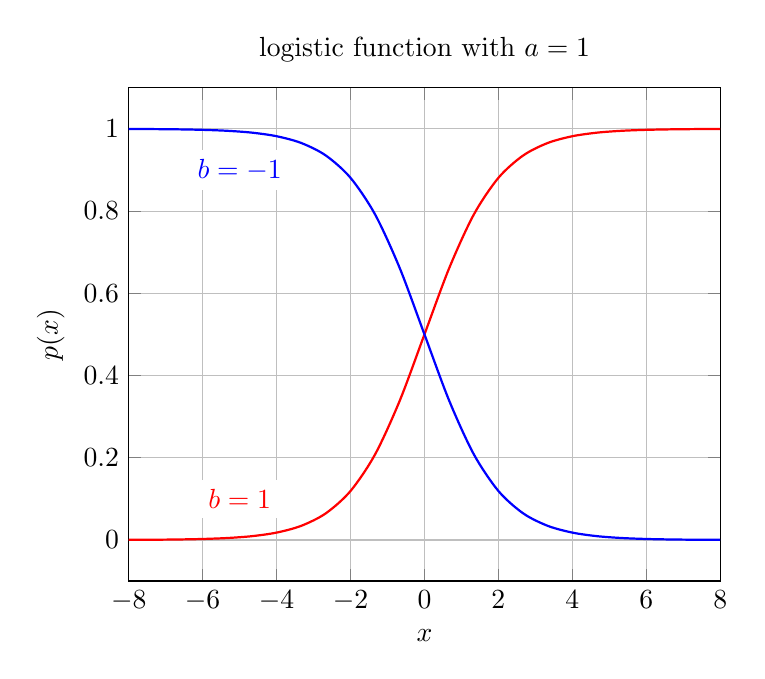
\begin{tikzpicture}
		\begin{axis}[width = 0.75\textwidth,xlabel=$x$, ylabel=$ p(x) $, grid = both, xmin = -8, xmax = 8, title = {logistic function with $ a = 1 $}]
			\addplot[thick, smooth, draw=red][name path = f1, domain = -8:8]{exp(x)/(1 + exp(x))};
			\addplot[thick, smooth, draw=blue][name path = f2, domain = -8:8]{exp(-x)/(1 + exp(-x))};
			
			
			\node[color=red, fill=white] at (axis cs: -5,.1) {$ b = 1 $};
			\node[color=blue, fill=white] at (axis cs: -5,.9) {$ b = -1 $};
			
			
		\end{axis}
	\end{tikzpicture}
\end{figure}


In order to find the maximum likelihood estimators, consider the joint PDF of a set of binary responses $ \{Y_1, \dots, Y_k\} $,

\begin{align}
	\log(P\{Y_i = y_i;\ i = 1,\dots,k\}) &= \sum\limits_{i = 1}^{k} y_i (a + bx_i) - \sum\limits_{i = 1}^{k} \log(1 + \exp(a +b x_i))
\end{align}

Even though an analytical minimization of the above expression is not possible, there are several iterative computational approaches possible.



%	\chapter{Regression}

\begin{enumerate}
	
\item Performing the linear regression using \texttt{scipy.stats.linregress} outputs. \\

\begin{figure}[H]
	\begin{subfigure}[l]{0.2\linewidth}
		\centering
		\begin{tabular}{@{}rr@{}}
			\toprule
			\multicolumn{2}{c}{\texttt{linRegressOutput}} \\
			\midrule
			$\beta_1$     &         1.206366 \\
			$\beta_0$ &         2.463493 \\
			$r$    &         0.985651 \\
			$p$    &         0.000007 \\
			\bottomrule
		\end{tabular}
	\end{subfigure}
	%
	\begin{subfigure}[]{0.8\linewidth}
		\centering
		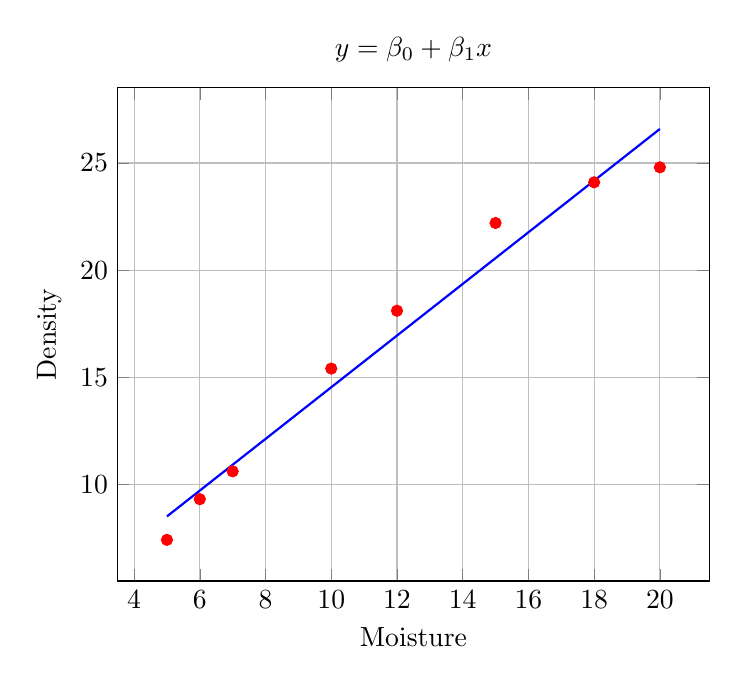
\begin{tikzpicture}
			\begin{axis}[width = 0.75\textwidth,xlabel= Moisture , ylabel= Density , grid=both, title = {$y = \beta_0 + \beta_1 x$}]
				\addplot[thick, smooth, draw=blue][domain= 5 : 20 ]{ 1.2064 *x +  2.4635 };
				\addplot[only marks, color = red] plot coordinates{(5, 7.4) (6, 9.3) (7, 10.6) (10, 15.4) (12, 18.1) (15, 22.2) (18, 24.1) (20, 24.8)};
			\end{axis}
		\end{tikzpicture}
	\end{subfigure}
\end{figure}

\item Performing the linear regression using \texttt{scipy.stats.linregress} outputs. \\
The value corresponding to $ x = 25 $ is $ y = 147.34 $.\\

\begin{figure}[H]
	\begin{subfigure}[]{0.2\linewidth}
		\centering
		\begin{tabular}{@{}rr@{}}
			\toprule
			\multicolumn{2}{c}{\texttt{linRegressOutput}} \\
			\midrule
			$\beta_1$     &    -2.376000e+00 \\
			$\beta_0$ &     2.067400e+02 \\
			$r$    &    -9.996792e-01 \\
			$p$    &     1.543680e-07 \\
			\bottomrule
		\end{tabular}
		
	\end{subfigure}
%
\begin{subfigure}[]{0.8\linewidth}
\centering

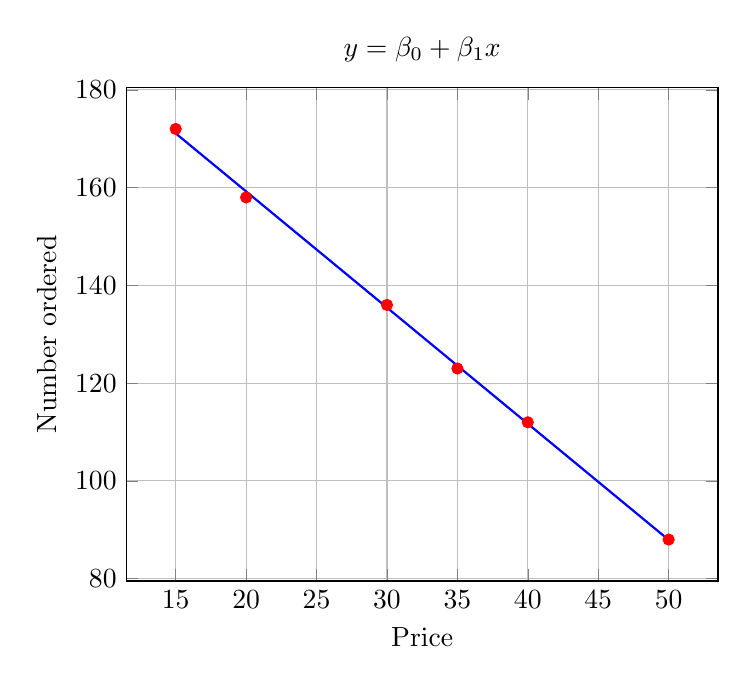
\begin{tikzpicture}
	\begin{axis}[width = 0.75\textwidth,xlabel= Price , ylabel= Number ordered , grid=both, title = {$y = \beta_0 + \beta_1 x$}]
		\addplot[thick, smooth, draw=blue][domain= 15.0 : 50.0 ]{ -2.376 *x +  206.74 };
		\addplot[only marks, color = red] plot coordinates{(50.0, 88.0) (40.0, 112.0) (35.0, 123.0) (30.0, 136.0) (20.0, 158.0) (15.0, 172.0)};
	\end{axis}
\end{tikzpicture}
	\end{subfigure}
\end{figure}

\item Performing the linear regression using \texttt{scipy.stats.linregress} outputs. \\
The value corresponding to $ x = 3.2 $ is $ y = 0.04476 $.\\

\begin{figure}[H]
	\begin{subfigure}[]{0.2\linewidth}
		\centering
		\begin{tabular}{@{}rr@{}}
			\toprule
			\multicolumn{2}{c}{\texttt{linRegressOutput}} \\
			\midrule
			$\beta_1$     &         0.011743 \\
			$\beta_0$ &         0.007186 \\
			$r$    &         0.995607 \\
			$p$    &         0.000029 \\
			\bottomrule
		\end{tabular}
		
	\end{subfigure}
	%
	\begin{subfigure}[]{0.8\linewidth}
		\centering
		
		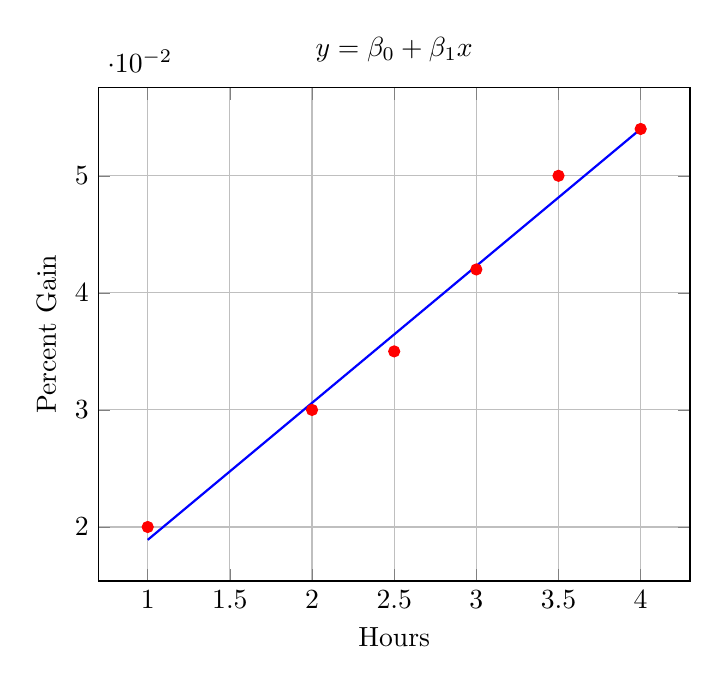
\begin{tikzpicture}
			\begin{axis}[width = 0.75\textwidth,xlabel=Hours, ylabel=Percent Gain, grid=both, title = {$y = \beta_0 + \beta_1 x$}]
				\addplot[thick, smooth, draw=blue][domain=1.0:4.0]{0.0117*x + 0.0072};
				\addplot[only marks, color = red] plot coordinates{(1.0, 0.02) (2.0, 0.03) (2.5, 0.035) (3.0, 0.042) (3.5, 0.05) (4.0, 0.054)};
			\end{axis}
		\end{tikzpicture}
	\end{subfigure}
\end{figure}
	
\item Performing the linear regression using \texttt{scipy.stats.linregress} outputs. \\
The value corresponding to $ x = 0.43 $ is $ y = 2439.75 $.\\

\begin{figure}[H]
	\begin{subfigure}[]{0.2\linewidth}
		\centering
		\begin{tabular}{@{}rr@{}}
			\toprule
			\multicolumn{2}{c}{\texttt{linRegressOutput}} \\
			\midrule
			$\beta_1$     &     12245.746692 \\
			$\beta_0$ &     -2825.916824 \\
			$r$    &         0.695796 \\
			$p$    &         0.025447 \\
			\bottomrule
		\end{tabular}
		
	\end{subfigure}
	%
	\begin{subfigure}[]{0.8\linewidth}
		\centering
		
		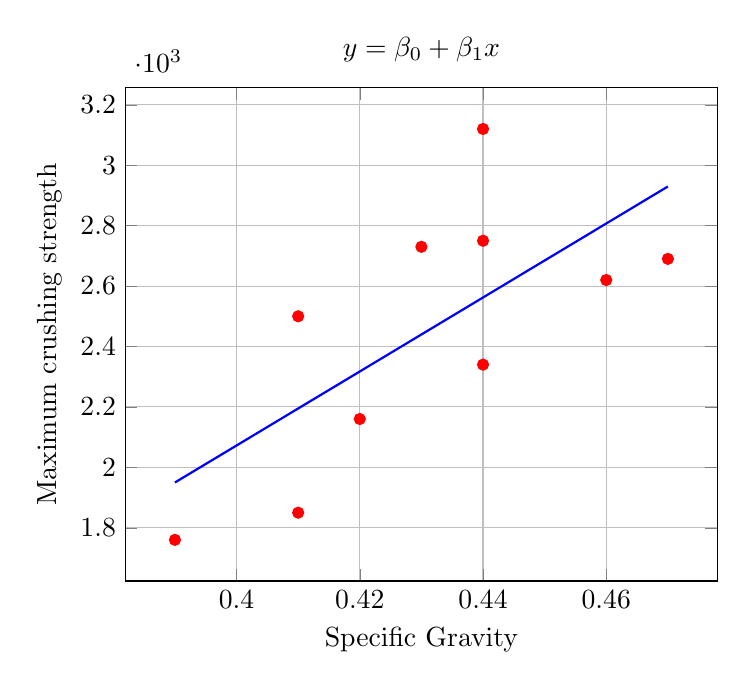
\begin{tikzpicture}
			\begin{axis}[width = 0.75\textwidth,xlabel=Specific Gravity, ylabel=Maximum crushing strength, grid=both, title = {$y = \beta_0 + \beta_1 x$}, scaled y ticks={base 10:-3}]
				\addplot[thick, smooth, draw=blue][domain=0.39:0.47]{12245.7467*x + -2825.9168};
				\addplot[only marks, color = red] plot coordinates{(0.39, 1760.0) (0.41, 1850.0) (0.41, 2500.0) (0.42, 2160.0) (0.43, 2730.0) (0.44, 2340.0) (0.44, 2750.0) (0.44, 3120.0) (0.46, 2620.0) (0.47, 2690.0)};
			\end{axis}
		\end{tikzpicture}
	\end{subfigure}
\end{figure}


\item Performing the linear regression using \texttt{scipy.stats.linregress} outputs. \\
The least squares estimators are $ A = 2.64 $ and $ B = 11.79 $.\\
The value corresponding to $ x = 7 $ is $ y = 85.22 $.\\

\begin{figure}[H]
	\begin{subfigure}[]{0.2\linewidth}
		\centering
		\begin{tabular}{@{}rr@{}}
			\toprule
			\multicolumn{2}{c}{\texttt{linRegressOutput}} \\
			\midrule
			$\beta_1$     &     1.179690e+01 \\
			$\beta_0$ &     2.638928e+00 \\
			$r$    &     9.931055e-01 \\
			$p$    &     9.803790e-09 \\
			\bottomrule
		\end{tabular}
		
	\end{subfigure}
	%
	\begin{subfigure}[]{0.8\linewidth}
		\centering
		
		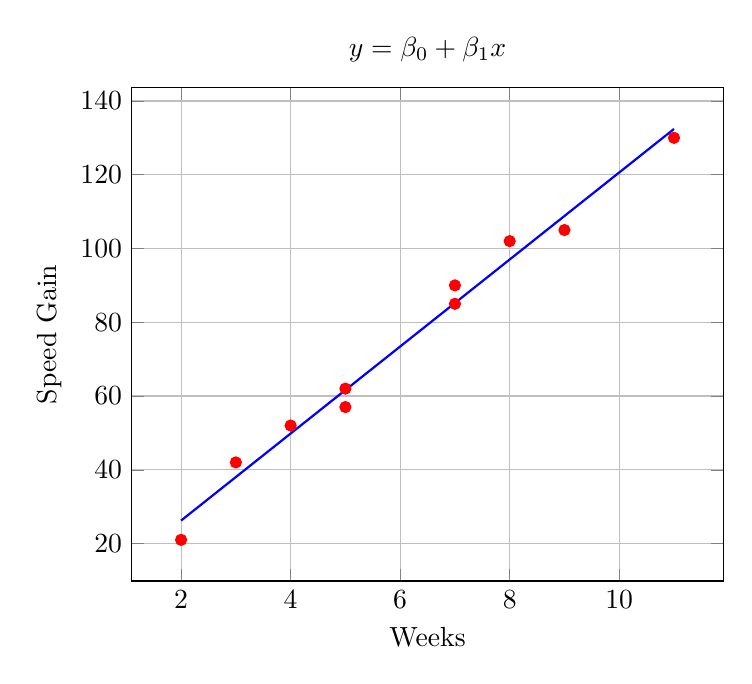
\begin{tikzpicture}
			\begin{axis}[width = 0.75\textwidth,xlabel=Weeks, ylabel=Speed Gain, grid=both, title = {$y = \beta_0 + \beta_1 x$}]
				\addplot[thick, smooth, draw=blue][domain=2.0:11.0]{11.7969*x + 2.6389};
				\addplot[only marks, color = red] plot coordinates{(2.0, 21.0) (3.0, 42.0) (4.0, 52.0) (5.0, 57.0) (5.0, 62.0) (7.0, 85.0) (7.0, 90.0) (8.0, 102.0) (9.0, 105.0) (11.0, 130.0)};
			\end{axis}
		\end{tikzpicture}
	\end{subfigure}
\end{figure}


\item Performing the linear regression using \texttt{scipy.stats.linregress} outputs. \\
The value corresponding to $ y = 1.15 $ is $ x = 57\% $.\\

\begin{figure}[H]
	\begin{subfigure}[]{0.2\linewidth}
		\centering
		\begin{tabular}{@{}rr@{}}
			\toprule
			\multicolumn{2}{c}{\texttt{linRegressOutput}} \\
			\midrule
			$\beta_1$     &         0.007026 \\
			$\beta_0$ &         0.749714 \\
			$r$    &         0.997906 \\
			$p$    &         0.000007 \\
			\bottomrule
		\end{tabular}
		
	\end{subfigure}
	%
	\begin{subfigure}[]{0.8\linewidth}
		\centering
		
		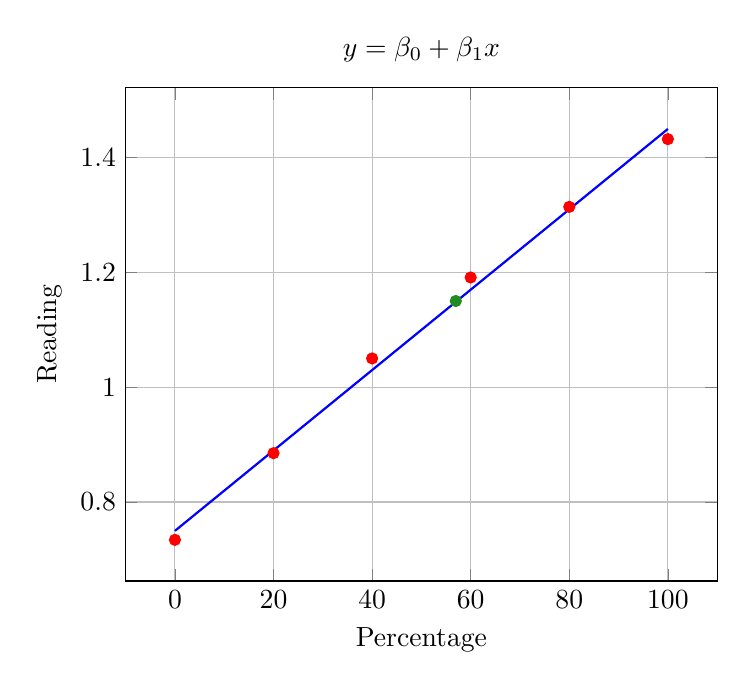
\begin{tikzpicture}
			\begin{axis}[width = 0.75\textwidth,xlabel=Percentage, ylabel=Reading, grid=both, title = {$y = \beta_0 + \beta_1 x$}]
				\addplot[thick, smooth, draw=blue][domain=0.0:100.0]{0.007*x + 0.7497};
				\addplot[only marks, color = red] plot coordinates{(0.0, 0.734) (20.0, 0.885) (40.0, 1.05) (60.0, 1.191) (80.0, 1.314) (100.0, 1.432)};
				\addplot[only marks, color = ForestGreen] plot coordinates{( 56.974379829198845 , 1.15 )};
			\end{axis}
		\end{tikzpicture}
	\end{subfigure}
\end{figure}


\item Performing the linear regression on the first 20 states using \texttt{scipy.stats.linregress} outputs. \\
The predicted values for the next 5 states are plotted. mean of the first 20 states' math scores is $ \overline{Y} = 525.7 $\\

\begin{figure}[H]
	\begin{subfigure}[]{0.2\linewidth}
		\centering
		\begin{tabular}{@{}rr@{}}
			\toprule
			\multicolumn{2}{c}{\texttt{linRegressOutput}} \\
			\midrule
			$\beta_1$     &    -1.212983e+00 \\
			$\beta_0$ &     5.689428e+02 \\
			$r$    &    -8.640923e-01 \\
			$p$    &     9.078458e-07 \\
			\bottomrule
		\end{tabular}
		
	\end{subfigure}
	%
	\begin{subfigure}[]{0.8\linewidth}
		\centering
		
		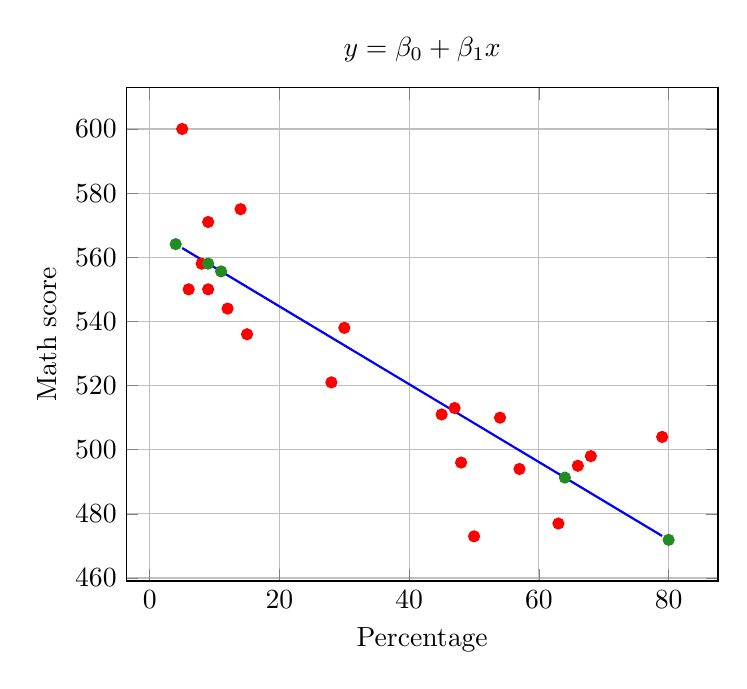
\begin{tikzpicture}
			\begin{axis}[width = 0.75\textwidth,xlabel=Percentage, ylabel=Math score, grid=both, title = {$y = \beta_0 + \beta_1 x$}]
				\addplot[thick, smooth, draw=blue][domain=5:79]{-1.213*x + 568.9428};
				\addplot[only marks, color = red] plot coordinates{(8, 558) (47, 513) (28, 521) (6, 550) (45, 511) (30, 538) (79, 504) (66, 495) (50, 473) (48, 496) (63, 477) (54, 510) (15, 536) (14, 575) (57, 494) (5, 600) (9, 571) (12, 544) (9, 550) (68, 498)};
				\addplot[only marks, color = ForestGreen] plot coordinates{(64, 491.311935572149) (80, 471.9042096163954) (11, 555.6000278005829) (9, 558.0259935450522) (4, 564.0909079062252)};
			\end{axis}
		\end{tikzpicture}
	\end{subfigure}
\end{figure}

\item Verifying the expression for $ \mathrm{Var}(A) $, \\

\begin{align}
	\mathrm{Var}(Y_i) &= \sigma^2 \nonumber \\
	%
	\mathrm{Var}(B) &= \frac{\mathrm{Var}\left[\sum (x_i - \overline{x})\ (Y_i - \overline{Y})\right]}{S_{xx}^2} \nonumber \\
	%
	&= \frac{\sum (x_i - \overline{x})^2\ \mathrm{Var}(Y_i - \overline{Y})}{S_{xx}^2} = \frac{\sigma^2}{S_{xx}} \\
	%
	\mathrm{Var}(A) &= \overline{x}^2\ \mathrm{Var}(B) + \frac{\mathrm{Var}\sum y_i}{n^2} + 2\ \mathrm{Cov}\left( \frac{\sum y_i}{n}\ ,\  -B \overline{x} \right) \nonumber \\
	%
	&= \frac{\sigma^2}{n} + \overline{x}^2 \frac{\sigma^2}{S_{xx}} - \frac{2B}{n} \ \mathrm{Cov}\left( \sum y_i\ ,\ B \right) \nonumber \\
	&= \frac{\sum x_i^2}{n}\ \frac{\sigma^2}{S_{xx}}
\end{align}\\

The covariance term vanishes as shown below.\\

\begin{align}
	\mathrm{Cov}\left( \sum y_i\ ,\ B \right) &= \sum\limits_{i = 1}^{n} \sum\limits_{j = 1}^{n} \mathrm{Cov}\left( y_i\ ,\ \frac{(x_j - \overline{x})\ y_j}{S_{xx}} \right) \nonumber \\
	%
	&= \frac{\sigma^2}{S_{xx}}\ \sum\limits_{i = 1}^{n} (x_i - \overline{x}) = 0
\end{align}\\


\item Using the data from Problem 4, \\

$ \sigma^2 $ = 105660 is a point estimate along with an interval estimate based on the $ \chi^2 $ distribution give by $ [54508, 309327] $\\

\item To prove the relation for $ SS_R $ using the previously defined shorthand notation\\
 $ S_{xx}, S_{YY}, S_{xY} $, \\

\begin{align}
	SS_R &= \sum (Y_i - A - B x_i)^2 = \sum(Y_i - \overline{Y} + B \overline{x} - B x_i)^2 \\
	%
	&= \sum (Y_i - \overline{Y})^2 + B^2\ \sum (\overline{x} - x_i)^2 + 2B\ \sum (Y_i - \overline{Y})(\overline{x} - x_i) \nonumber \\
	%
	&= S_{YY} + \frac{S_{xY}^2}{S_{xx}} - 2\ \frac{S_{xY}^2}{S_{xx}} \nonumber \\
	%
	&= \frac{S_{xx}S_{YY} - S_{xY}^2}{S_{xx}}
\end{align}\\

\item Performing the linear regression using \texttt{scipy.stats.linregress} outputs. \\
Testing the hypothesis that $ \beta_1 = 0 $ gives a p-value of $ 1.6\% $. The hypothesis can be rejected at $ 5\% $ confidence level.\\


\begin{figure}[H]
	\begin{subfigure}[]{0.2\linewidth}
		\centering
		\begin{tabular}{@{}rr@{}}
			\toprule
			\multicolumn{2}{c}{\texttt{linRegressOutput}} \\
			\midrule
			$\beta_1$     &         0.047795 \\
			$\beta_0$ &        46.466853 \\
			$r$    &         0.626258 \\
			$p$    &         0.016568 \\
			\bottomrule
		\end{tabular}
		
	\end{subfigure}
	%
	\begin{subfigure}[]{0.8\linewidth}
		\centering
		
		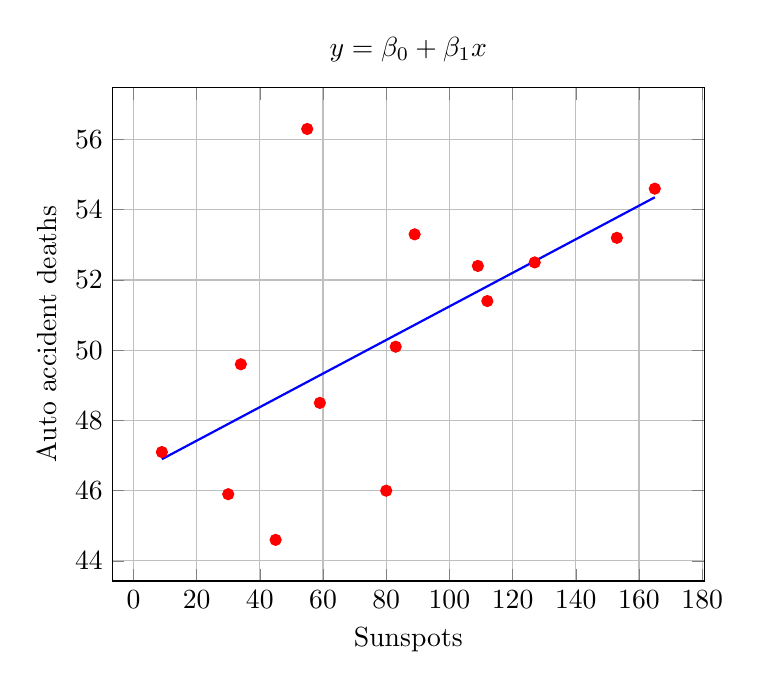
\begin{tikzpicture}
			\begin{axis}[width = 0.75\textwidth,xlabel=Sunspots, ylabel=Auto accident deaths, grid=both, title = {$y = \beta_0 + \beta_1 x$}]
				\addplot[thick, smooth, draw=blue][domain=9:165]{0.0478*x + 46.4669};
				\addplot[only marks, color = red] plot coordinates{(9, 47.1) (30, 45.9) (34, 49.6) (45, 44.6) (55, 56.3) (59, 48.5) (80, 46.0) (83, 50.1) (89, 53.3) (109, 52.4) (112, 51.4) (127, 52.5) (153, 53.2) (165, 54.6)};
			\end{axis}
		\end{tikzpicture}
	\end{subfigure}
\end{figure}

\item Performing the linear regression using \texttt{scipy.stats.linregress} outputs. \\
Testing the hypothesis that $ \beta_1 = 0 $ gives a p-value of $ 11.1\% $. The hypothesis cannot be rejected at $ 5\% $ confidence level. This means that salary is not related to height.\\

\begin{figure}[H]
	\begin{subfigure}[]{0.2\linewidth}
		\centering
		\begin{tabular}{@{}rr@{}}
			\toprule
			\multicolumn{2}{c}{\texttt{linRegressOutput}} \\
			\midrule
			$\beta_1$     &         1.457143 \\
			$\beta_0$ &        -4.985714 \\
			$r$    &         0.483846 \\
			$p$    &         0.110981 \\
			\bottomrule
		\end{tabular}
		
	\end{subfigure}
	%
	\begin{subfigure}[]{0.8\linewidth}
		\centering
		
		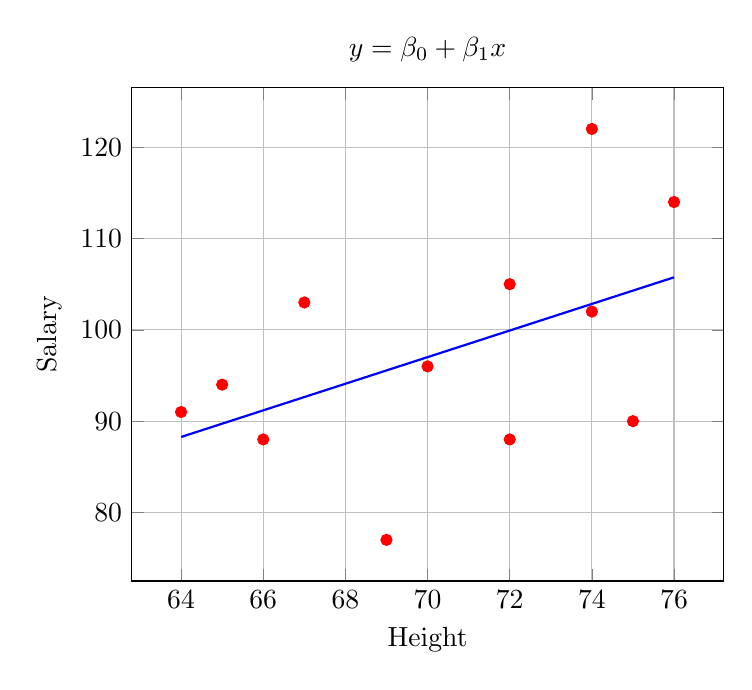
\begin{tikzpicture}
			\begin{axis}[width = 0.75\textwidth,xlabel=Height, ylabel=Salary, grid=both, title = {$y = \beta_0 + \beta_1 x$}]
				\addplot[thick, smooth, draw=blue][domain=64:76]{1.4571*x + -4.9857};
				\addplot[only marks, color = red] plot coordinates{(64, 91) (65, 94) (66, 88) (67, 103) (69, 77) (70, 96) (72, 105) (72, 88) (74, 122) (74, 102) (75, 90) (76, 114)};
			\end{axis}
		\end{tikzpicture}
	\end{subfigure}
\end{figure}

\item Given $ 0 < \beta < 1 $ in a simple linear regression model.

\begin{enumerate}
	\item \begin{align}
		x &< \frac{\alpha}{(1 - \beta)} \to x < \alpha + \beta x \nonumber \\
		%
		\mathbb{E}[Y_i] &= \alpha + \beta x \to \mathbb{E}[Y] > x \nonumber \\
		%
		\mathbb{E}[Y] &< \frac{\alpha}{1 - \beta} \qquad \text{obvious}	\\
		%
		\therefore x &< \mathbb{E}[Y] < \frac{\alpha}{1 - \beta}			
	\end{align}

	\item Same as previous part with all inequalities reversed. This proves that $ \mathbb{E}[Y] $ always lies in between these two values.
	
	\begin{figure}[H]
		\centering
		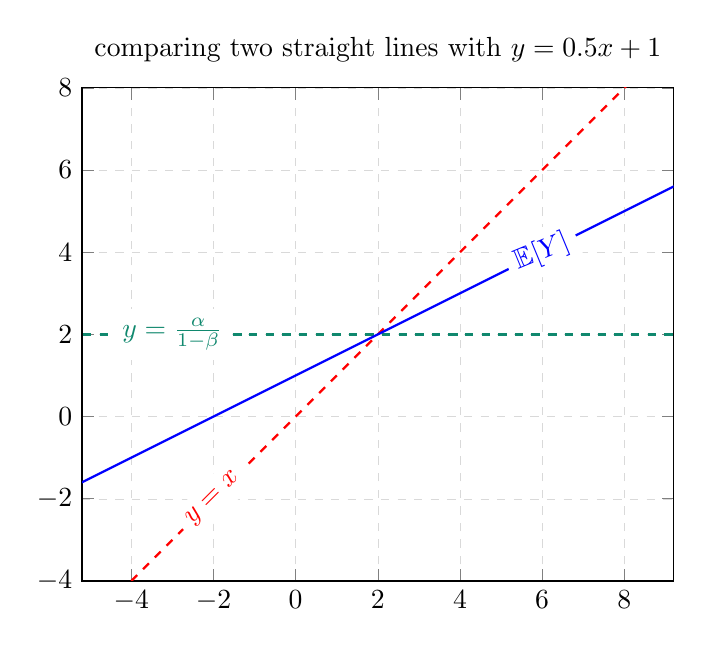
\begin{tikzpicture}
			\begin{axis}[axis equal, grid = both, grid style={line width=.1pt, draw=gray!30, dashed},
				 width = 0.75\textwidth, xmin = -4, xmax = 8, ymin = -4, ymax = 8, title = {comparing two straight lines with $ y = 0.5x + 1$}]
				\addplot[thick, smooth, draw=red, dashed][name path = f1, domain = -8:10]{x};
				\addplot[thick, smooth, draw=PineGreen, dashed][name path = f1, domain = -8:10]{2};
				\addplot[thick, smooth, draw=blue][name path = f2, domain = -8:10]{0.5*x + 1};
				
				
				\node[color=PineGreen, fill=white] at (axis cs: -3,2) {$ y = \frac{\alpha}{1 - \beta} $};
				\node[color=red, rotate = 45, fill=white] at (axis cs: -2,-2) {$ y = x $};
				\node[color=blue, rotate = 22.5, fill=white] at (axis cs: 6,4) {$ \mathbb{E}[Y] $};
				
							\end{axis}
		\end{tikzpicture}
	\end{figure}

\end{enumerate}

\item Given a linear regression $ Y = 0.159 + 0.4X + e $, with $ e \sim \mathcal{N}(0, \sigma^2) $. The predictions are outlined in the figure below.\\

\begin{figure}[H]
	\begin{subfigure}[]{0.2\linewidth}
		\centering
		\begin{tabular}{@{}rr@{}}
			\toprule
			$X$     &    $ Y $ \\
			\midrule
			  0.200  &  0.239    \\
			 0.265	&  0.265   \\
			  0.310  &  0.283  \\
			\bottomrule
		\end{tabular}
		
	\end{subfigure}
	%
	\begin{subfigure}[]{0.8\linewidth}
		\centering
		
		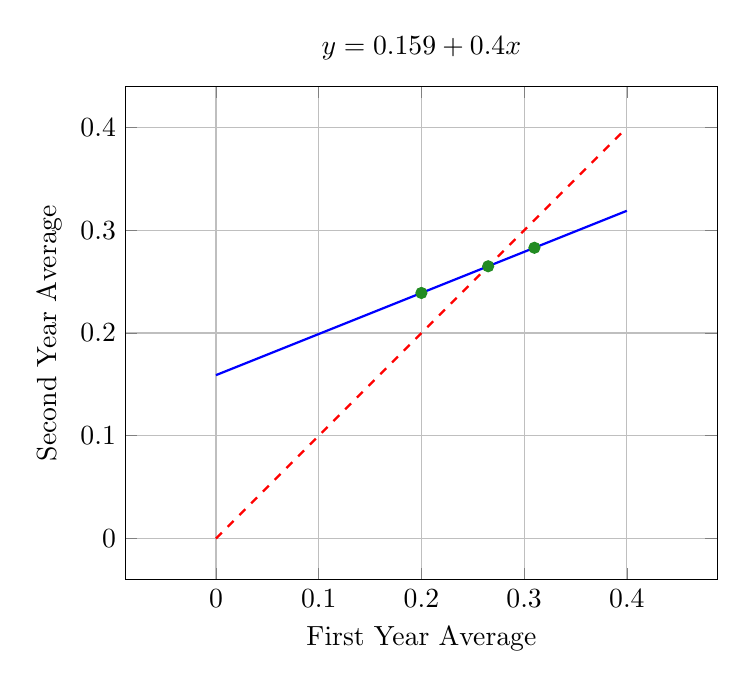
\begin{tikzpicture}
			\begin{axis}[axis equal, width = 0.75\textwidth, xlabel=First Year Average, ylabel=Second Year Average, grid=both, title = {$y = 0.159 + 0.4 x$}]
				\addplot[thick, smooth, draw=blue][domain=0:0.4]{0.159 + 0.4*x};
				\addplot[thick, smooth, draw=red, dashed][name path = f1, domain = 0:0.4]{x};
				\addplot[only marks, color = ForestGreen] plot coordinates{(0.2, 0.239) (0.265, 0.265) (0.31, 0.283)};
			\end{axis}
		\end{tikzpicture}
	\end{subfigure}
\end{figure}

\item This is a case of gambler's fallacy. When successive events are independent, it is possible merely through chance for successive outcomes to be good or bad without any causal effect of one outcome on the next. For example, tossing a coin 10 times can result in 10 heads just by chance.\\

\item In order to rearrange the estimator $ A $ of the regression parameter $ \alpha $ into a t-RV with $ n-2 $ DOF, \\

\begin{align}
	A &\sim \mathcal{N}\left(\alpha\ ,\ \frac{\sigma^2}{S_{xx}}\ \frac{\sum x_i^2}{n}\right) \nonumber \\
	%
	\frac{(A - \alpha)}{\sigma} \sqrt{\frac{nS_{xx}}{\sum x_i^2}} &\sim Z \\ 
	%
	\frac{SS_R}{\sigma^2} &\sim \chi^2_{n-2} \nonumber \\
	%
	\frac{1}{\sigma} \sqrt{\frac{SS_R}{n-2}} &\sim \sqrt{\frac{\chi^2_{n-2}}{(n-2)}}
\end{align}\\

Rearranging into a t-RV proves the result.\\

\begin{align}
	t_{n-2} &\sim \frac{Z}{\sqrt{\chi^2_{n-2} / (n-2)}} \nonumber \\
	%	
	t_{n-2} &\sim (A - \alpha)\ \sqrt{\frac{n(n-2)S_{xx}}{SS_R \sum x_i^2}}
\end{align}\\

\item Performing the linear regression using \texttt{scipy.stats.linregress} outputs. \\
The value corresponding to $ x = 24 $ is $ y = 12.604 $.\\

\begin{figure}[H]
	\begin{subfigure}[]{0.2\linewidth}
		\centering
		\begin{tabular}{@{}rr@{}}
			\toprule
			\multicolumn{2}{c}{\texttt{linRegressOutput}} \\
			\midrule
			$\beta_1$     &     5.528289e-01 \\
			$\beta_0$ &    -6.639400e-01 \\
			$r$    &     9.840458e-01 \\
			$p$    &     2.780621e-07 \\
			\bottomrule
		\end{tabular}
		
	\end{subfigure}
	%
	\begin{subfigure}[]{0.8\linewidth}
		\centering
		
		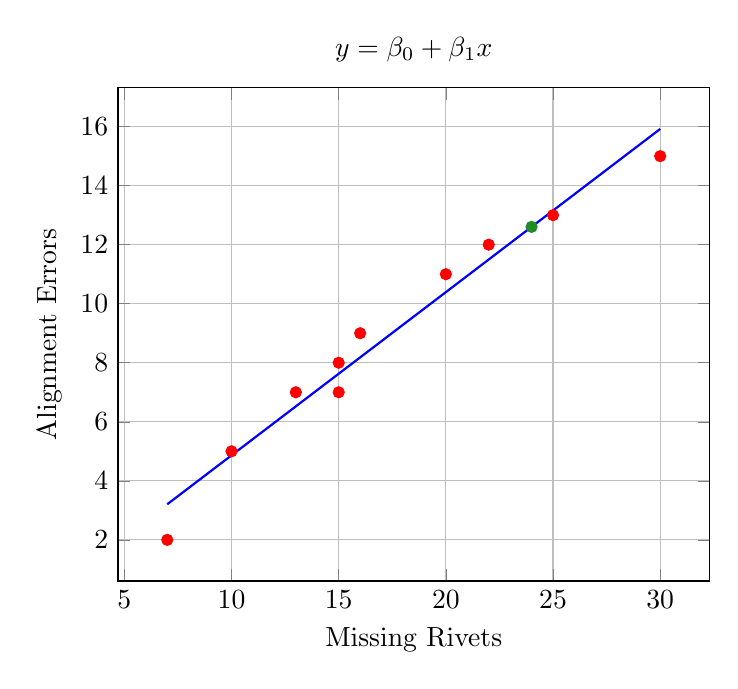
\begin{tikzpicture}
			\begin{axis}[width = 0.75\textwidth,xlabel=Missing Rivets, ylabel=Alignment Errors, grid=both, title = {$y = \beta_0 + \beta_1 x$}]
				\addplot[thick, smooth, draw=blue][domain=7:30]{0.5528*x + -0.6639};
				\addplot[only marks, color = red] plot coordinates{(7, 2) (10, 5) (13, 7) (15, 7) (15, 8) (16, 9) (20, 11) (22, 12) (25, 13) (30, 15)};
				\addplot[only marks, color = ForestGreen] plot coordinates{ (24, 12.603953646898432) };
			\end{axis}
		\end{tikzpicture}
	\end{subfigure}
\end{figure}

Hypothesis testing with $ \gamma = 10\% $ for $ H_0 : \alpha = 1 $ gives a p-value of $ 3.46\% $. This means that the hypothesis can be rejected.

\begin{align}
	H_0 : \alpha = 1 \qquad &\text{vs.} \qquad H_1 : \alpha \neq 1 \nonumber \\
	%
	\text{reject $ H_0 $ if } \qquad & \sqrt{\frac{n(n-2) S_{xx}}{SS_R\ \sum x_i^2}}\ |A - \alpha| > t_{\gamma/2, n-2} \nonumber \\
	%
	\text{accept $ H_0 $  } \qquad & \text{otherwise}
\end{align}\\

In order to find a confidence interval for $ x_0 = 24 $, using the above t-test, \\

\begin{align}
	Y(x_0) &\in A + B x_0 \pm t_{\gamma/2, n-2}\ \sqrt{\left(\frac{SS_R}{n-2}\right)\ \left(\frac{1}{n} + \frac{(x_0  - \overline{x})^2}{S_{xx}}\right)} \nonumber \\
	%
	Y(x_0) &\in 12.604 \pm 0.6196 = [11.98, 13.22]
\end{align}

\item Performing the linear regression using \texttt{scipy.stats.linregress} outputs. \\

\begin{figure}[H]
	\begin{subfigure}[]{0.2\linewidth}
		\centering
		\begin{tabular}{@{}rr@{}}
			\toprule
			\multicolumn{2}{c}{\texttt{linRegressOutput}} \\
			\midrule
			$\beta_1$     &         0.779935 \\
			$\beta_0$ &     -1047.614887 \\
			$r$    &         0.799131 \\
			$p$    &         0.009766 \\
			\bottomrule
		\end{tabular}
		
	\end{subfigure}
	%
	\begin{subfigure}[]{0.8\linewidth}
		\centering
		
		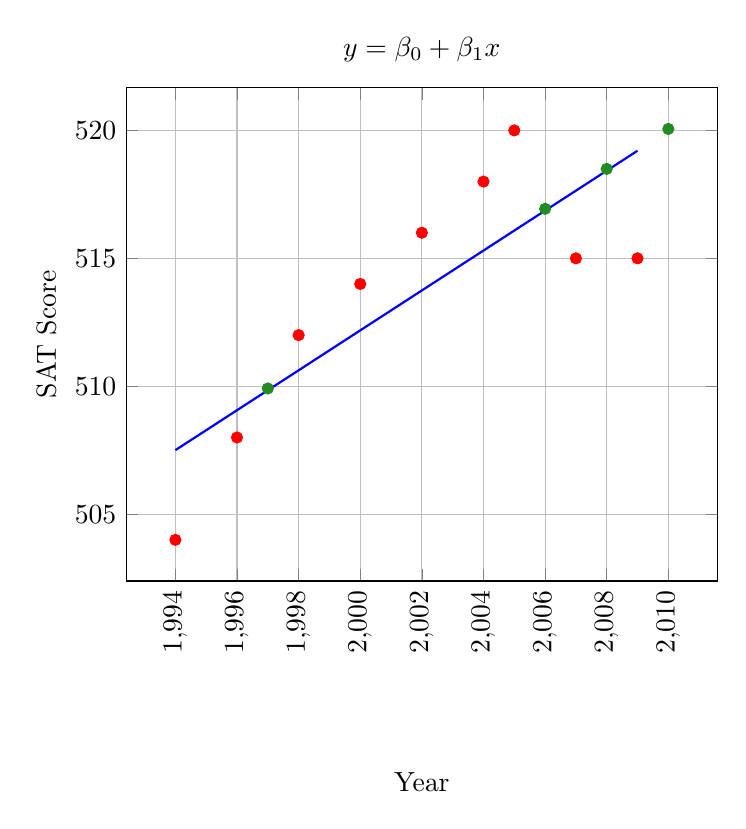
\begin{tikzpicture}
			\begin{axis}[width = 0.75\textwidth,xlabel=Year, ylabel=SAT Score, grid=both, title = {$y = \beta_0 + \beta_1 x$}, xticklabel style ={rotate=90}, xlabel style = {yshift = -0.5in}]
				\addplot[thick, smooth, draw=blue][domain=1994:2009]{0.7799*x + -1047.6149};
				\addplot[only marks, color = red] plot coordinates{(1994, 504) (1996, 508) (1998, 512) (2000, 514) (2002, 516) (2004, 518) (2005, 520) (2007, 515) (2009, 515)};
				\addplot[only marks, color = ForestGreen] plot coordinates{ (1997, 509.91585760517796)(2006, 516.935275080906)(2008, 518.4951456310678)(2010, 520.0550161812296) };
			\end{axis}
		\end{tikzpicture}
	\end{subfigure}
\end{figure}

The predicted values are as tabulated as \\
\begin{table}[H]
	\centering
	\begin{tabular}{@{}rr@{}}
		\toprule
		$ X $ & $ Y $ \\
		\midrule
		1997     &509.90\\
		2006 &  516.93  \\
		2008    &     518.49 \\
		2010   &  520.05 \\
		\bottomrule
	\end{tabular}
\end{table}

\item Performing the linear regression using \texttt{scipy.stats.linregress} outputs for bladder cancer. \\
Linear relationship is not very strong with p-value of $ 0.4\% $\\
The value corresponding to $ x = 2500 $ is $ y = 3.96 $.\\

\begin{figure}[H]
	\begin{subfigure}[]{0.2\linewidth}
		\centering
		\begin{tabular}{@{}rr@{}}
			\toprule
			\multicolumn{2}{c}{\texttt{linRegressOutput}} \\
			\midrule
			$\beta_1$     &         0.001241 \\
			$\beta_0$ &         0.859260 \\
			$r$    &         0.785832 \\
			$p$    &         0.004140 \\
			\bottomrule
		\end{tabular}
		
	\end{subfigure}
	%
	\begin{subfigure}[]{0.8\linewidth}
		\centering
		
		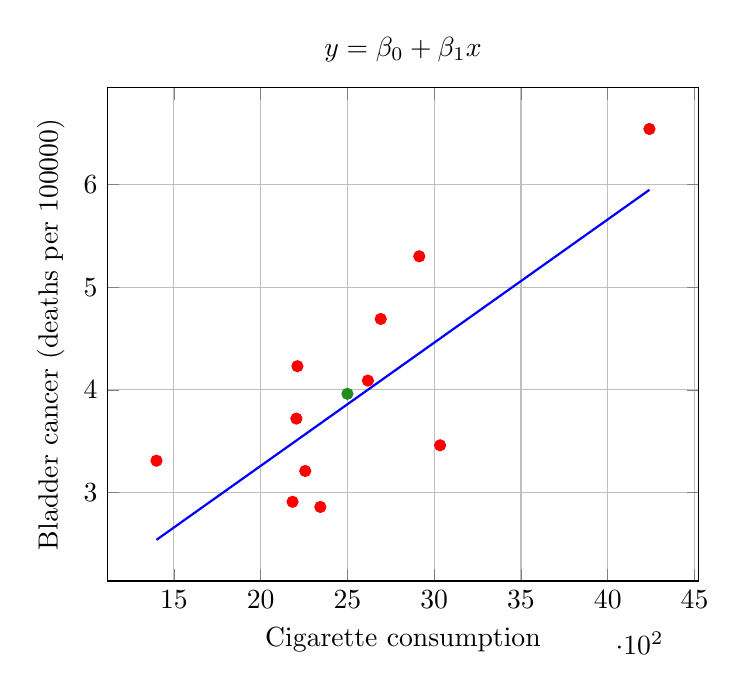
\begin{tikzpicture}
			\begin{axis}[width = 0.75\textwidth,xlabel=Cigarette consumption, ylabel=Bladder cancer (deaths per 100000), grid=both, title = {$y = \beta_0 + \beta_1 x$}, scaled x ticks={base 10:-2}]
				\addplot[thick, smooth, draw=blue][domain=1400:4240]{0.0012*x + 0.8593};
				\addplot[only marks, color = red] plot coordinates{(1400, 3.31) (2184, 2.91) (2206, 3.72) (2212, 4.23) (2257, 3.21) (2344, 2.86) (2618, 4.09) (2692, 4.69) (2914, 5.3) (3034, 3.46) (4240, 6.54)};
				\addplot[only marks, color = ForestGreen] plot coordinates{ (2500, 3.9612972876385455) };
			\end{axis}
		\end{tikzpicture}
	\end{subfigure}
\end{figure}

\item Performing the linear regression using \texttt{scipy.stats.linregress} outputs for lung cancer. \\
Linear relationship is very strong with p-value of $ 0.67\% $\\
The value corresponding to $ x = 2500 $ is $ y = 3.96 $.\\

\begin{figure}[H]
	\begin{subfigure}[]{0.2\linewidth}
		\centering
		\begin{tabular}{@{}rr@{}}
			\toprule
			\multicolumn{2}{c}{\texttt{linRegressOutput}} \\
			\midrule
			$\beta_1$     &         0.004715 \\
			$\beta_0$ &         7.443316 \\
			$r$    &         0.759411 \\
			$p$    &         0.006706 \\
			\bottomrule
		\end{tabular}
		
	\end{subfigure}
	%
	\begin{subfigure}[]{0.8\linewidth}
		\centering
		
		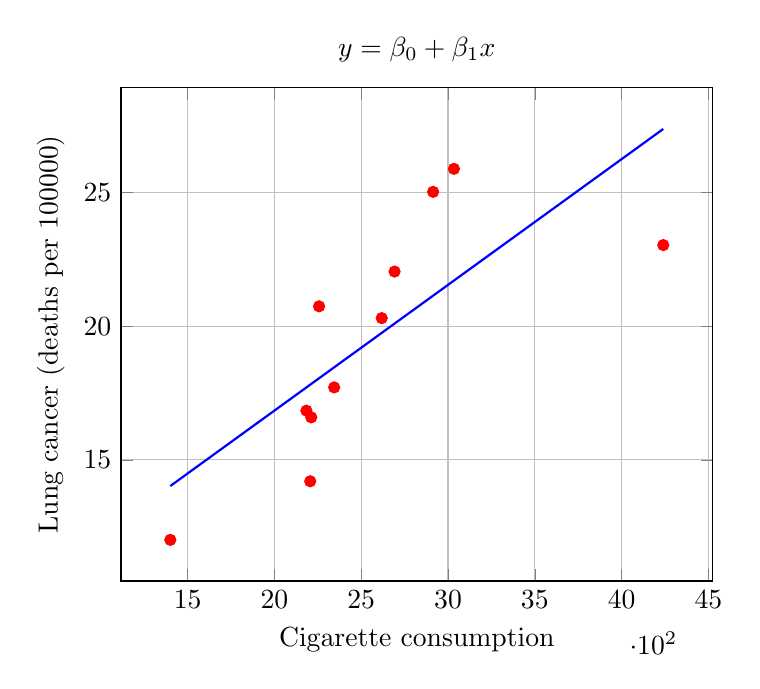
\begin{tikzpicture}
			\begin{axis}[width = 0.75\textwidth,xlabel=Cigarette consumption, ylabel=Lung cancer (deaths per 100000), grid=both, title = {$y = \beta_0 + \beta_1 x$}, scaled x ticks={base 10:-2}]
				\addplot[thick, smooth, draw=blue][domain=1400:4240]{0.0047*x + 7.4433};
				\addplot[only marks, color = red] plot coordinates{(1400, 12.01) (2184, 16.84) (2206, 14.2) (2212, 16.59) (2257, 20.74) (2344, 17.71) (2618, 20.3) (2692, 22.04) (2914, 25.02) (3034, 25.88) (4240, 23.03)};
			\end{axis}
		\end{tikzpicture}
	\end{subfigure}
\end{figure}

\item Performing the linear regression using \texttt{scipy.stats.linregress} outputs for kidney cancer. \\
Linear relationship is nonexistent with p-value of $ 29\% $\\
The value corresponding to $ x = 2500 $ is $ y = 3.96 $.\\

\begin{figure}[H]
	\begin{subfigure}[]{0.2\linewidth}
		\centering
		\begin{tabular}{@{}rr@{}}
			\toprule
			\multicolumn{2}{c}{\texttt{linRegressOutput}} \\
			\midrule
			$\beta_1$     &         0.000296 \\
			$\beta_0$ &         2.194573 \\
			$r$    &         0.351066 \\
			$p$    &         0.289780 \\
			\bottomrule
		\end{tabular}
		
	\end{subfigure}
	%
	\begin{subfigure}[]{0.8\linewidth}
		\centering
		
		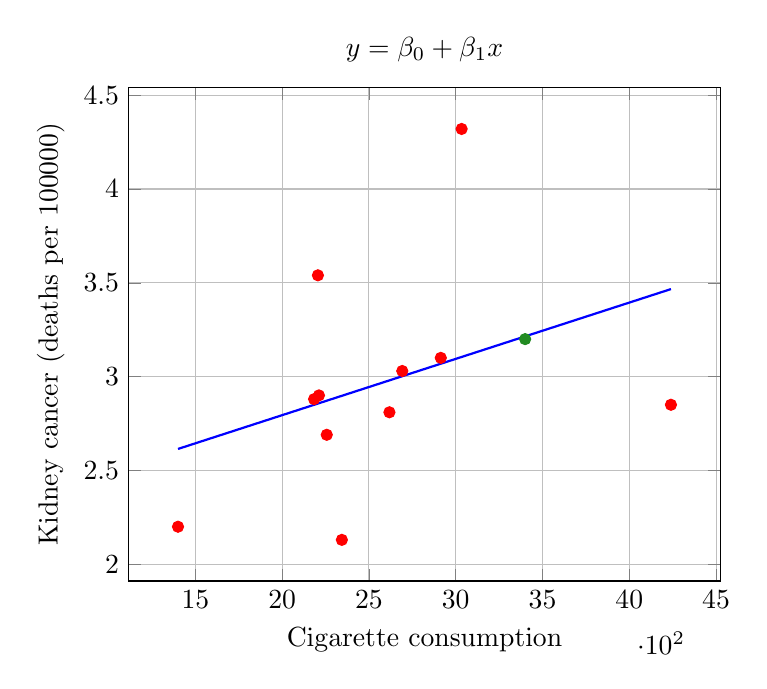
\begin{tikzpicture}
			\begin{axis}[width = 0.75\textwidth,xlabel=Cigarette consumption, ylabel=Kidney cancer (deaths per 100000), grid=both, title = {$y = \beta_0 + \beta_1 x$}, scaled x ticks={base 10:-2}]
				\addplot[thick, smooth, draw=blue][domain=1400:4240]{0.0003*x + 2.1946};
				\addplot[only marks, color = red] plot coordinates{(1400, 2.2) (2184, 2.88) (2206, 3.54) (2212, 2.9) (2257, 2.69) (2344, 2.13) (2618, 2.81) (2692, 3.03) (2914, 3.1) (3034, 4.32) (4240, 2.85)};
				\addplot[only marks, color = ForestGreen] plot coordinates{ (3400, 3.2) };
			\end{axis}
		\end{tikzpicture}
	\end{subfigure}
\end{figure}

The $ 90\% $ confidence interval for the mean death rate with $ x_0 = 3400 $ is given by \\
$ Y(x_0) = 3.2 \pm 0.52 = [2.67, 3.72] $\\


\item Performing the linear regression using \texttt{scipy.stats.linregress} outputs for leukemia. \\
Linear relationship is nonexistent with p-value of $ 35.31\% $ for the hypothesis $ H_0 : \beta = 0 $\\
The value corresponding to $ x = 2500 $ is $ y = 3.96 $.\\
The $ 90\% $ confidence interval for the mean death rate with $ x_0 = 2500 $ is given by \\
$ Y(x_0) = 6.95 \pm 0.47 = [6.48, 7.42] $\\

\begin{figure}[H]
	\begin{subfigure}[]{0.2\linewidth}
		\centering
		\begin{tabular}{@{}rr@{}}
			\toprule
			\multicolumn{2}{c}{\texttt{linRegressOutput}} \\
			\midrule
			$\beta_1$     &        -0.000371 \\
			$\beta_0$ &         7.877593 \\
			$r$    &        -0.310281 \\
			$p$    &         0.353081 \\
			\bottomrule
		\end{tabular}
		
	\end{subfigure}
	%
	\begin{subfigure}[]{0.8\linewidth}
		\centering
		
		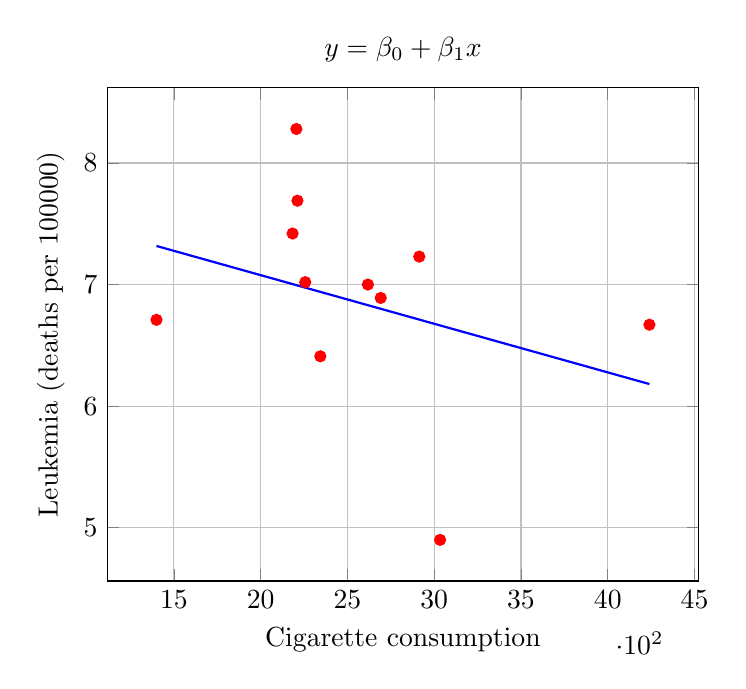
\begin{tikzpicture}
			\begin{axis}[width = 0.75\textwidth,xlabel=Cigarette consumption, ylabel=Leukemia (deaths per 100000), grid=both, title = {$y = \beta_0 + \beta_1 x$}, scaled x ticks={base 10:-2}]
				\addplot[thick, smooth, draw=blue][domain=1400:4240]{-0.0004*x + 7.8776};
				\addplot[only marks, color = red] plot coordinates{(1400, 6.71) (2184, 7.42) (2206, 8.28) (2212, 7.69) (2257, 7.02) (2344, 6.41) (2618, 7.0) (2692, 6.89) (2914, 7.23) (3034, 4.9) (4240, 6.67)};
			\end{axis}
		\end{tikzpicture}
	\end{subfigure}
\end{figure}

\item The variances along with the $ 95\% $ confidence intervals are as follows,\\

The predicted values are as tabulated as \\
\begin{table}[H]
	\centering
	\begin{tabular}{@{}lrr@{}}
		\toprule
		Disease		& $ \sigma^2 $	& Interval \\
		\midrule
		Bladder Cancer	& 0.54	& [0.2538, 1.7884]\\
		Lung Cancer	& 9.18	& [4.3436, 30.5983]\\
		Kidney Cancer	& 0.35	& [0.1656, 1.1667]\\
		Leukemia	& 0.73	& [0.3445, 2.4270]\\
		\bottomrule
	\end{tabular}
\end{table}

The variance for the two sets of data are $ \sigma_1^2 = 6.56 $ and $ \sigma_2^2 = 9.02 $. Since the two variances can be arranged into $ \chi^2 $ RVs, their ratio is an f-RV and this can be used to perform the significance test.

\begin{align}
	\frac{SS_{R1}}{\sigma_1^2}\ \frac{\sigma_2^2}{SS_{R2}} &\sim \frac{\chi^2_{n-2}}{\chi^2_{m-2}} \nonumber \\
	%
	\frac{SS_{R1}}{\sigma_1^2}\ \frac{\sigma_2^2}{SS_{R2}}\ \frac{m-2}{n-2} &\sim f_{n-2, m-2}
\end{align}\\

Using the above f-test, the p-value for equality of the two variances is $ 95.78\% $. This is sufficient to reject the alternative hypothesis at the $ 5\% $ confidence level.\\

\item Plotting standardized residuals shows that the assumption of linearity is reasonable. There are no discernible trends among the residual data points.\\

\begin{figure}[H]
	\centering
	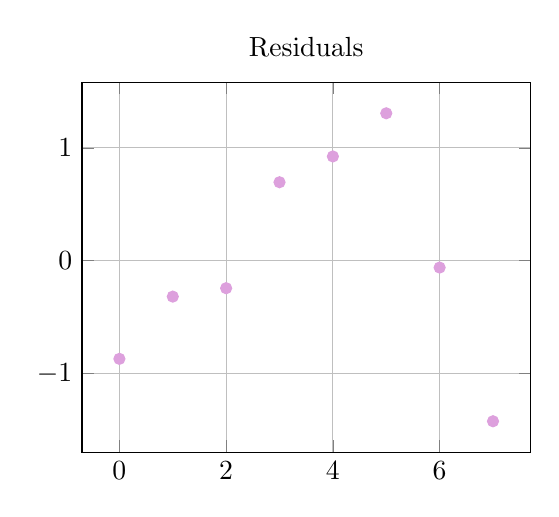
\begin{tikzpicture}
		\begin{axis}[width = 0.6\textwidth, grid=both, title = {Residuals}]
			\addplot[only marks, color = Plum] plot coordinates{(0, -0.8718640529850565) (1, -0.3197402889509025) (2, -0.24520896212952864) (3, 0.6947736741537625) (4, 0.9234350673319759) (5, 1.3062265268670226) (6, -0.06215428337811557) (7, -1.4254676809091682)};
		\end{axis}
	\end{tikzpicture}
\end{figure}

\item $ R = r^2 = 0.999625 $. \\
p-value is so small for the linear regression that non-linearity can be strongly rejected, although there is a clear pattern in the residuals plot.\\
The $ 90\% $ confidence interval for the amount of protein with $ x_0 = 1.5 $ is given by \\
$ Y(x_0) = 41.97 \pm 1.2834 = [40.69, 43.26] $\\

\begin{figure}[H]
	\begin{subfigure}[]{0.2\linewidth}
		\centering
		\begin{tabular}{@{}rr@{}}
			\toprule
			\multicolumn{2}{c}{\texttt{linRegressOutput}} \\
			\midrule
			$\beta_1$     &        38.046693 \\
			$\beta_0$ &       -15.095097 \\
			$r$    &         0.999813 \\
			$p$    &         0.000003 \\
			\bottomrule
		\end{tabular}
		
	\end{subfigure}
	%
	\begin{subfigure}[]{0.8\linewidth}
		\centering
		
		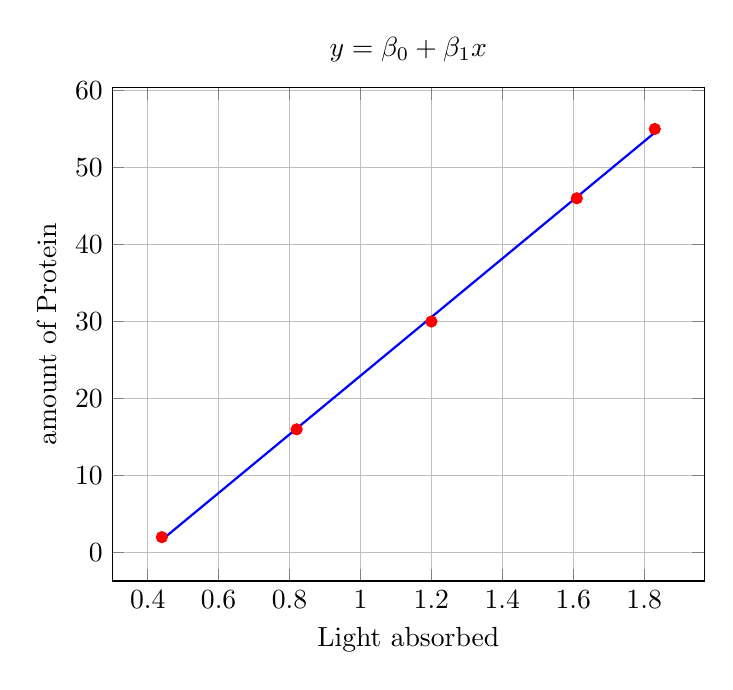
\begin{tikzpicture}
			\begin{axis}[width = 0.75\textwidth,xlabel=Light absorbed, ylabel=amount of Protein, grid=both, title = {$y = \beta_0 + \beta_1 x$}]
				\addplot[thick, smooth, draw=blue][domain=0.44:1.83]{38.0467*x + -15.0951};
				\addplot[only marks, color = red] plot coordinates{(0.44, 2) (0.82, 16) (1.2, 30) (1.61, 46) (1.83, 55)};
			\end{axis}
		\end{tikzpicture}
	\end{subfigure}
\end{figure}

\begin{figure}[H]
	\centering
	\begin{tikzpicture}
		\begin{axis}[width = 0.6\textwidth, grid=both, title = {Residuals}]
			\addplot[only marks, color = Plum] plot coordinates{(0, 0.7354666946526062) (1, -0.2140537394883921) (2, -1.1635741736293976) (3, -0.3320577240782377) (4, 0.9742189425434361)};
		\end{axis}
	\end{tikzpicture}
\end{figure}	

\item The hypothesis $ H_0 : \beta = 1 $ has a p-value of 2.55\% and thus can be rejected at the 5\% level of significance.\\

\begin{figure}[H]
	\begin{subfigure}[]{0.2\linewidth}
		\centering
		\begin{tabular}{@{}rr@{}}
			\toprule
			\multicolumn{2}{c}{\texttt{linRegressOutput}} \\
			\midrule
			$\beta_1$     &     9.927803e-01 \\
			$\beta_0$ &    -2.221420e+01 \\
			$r$    &     9.999718e-01 \\
			$p$    &     2.771209e-18 \\
			\bottomrule
		\end{tabular}
		
	\end{subfigure}
	%
	\begin{subfigure}[]{0.8\linewidth}
		\centering
		
		\begin{tikzpicture}
			\begin{axis}[width = 0.75\textwidth,xlabel=Weld diameter, ylabel=Shear strength, grid=both, title = {$y = \beta_0 + \beta_1 x$}, scaled y ticks={base 10:-3}, scaled x ticks={base 10:-2}]
				\addplot[thick, smooth, draw=blue][domain=400:4000]{0.9928*x + -22.2142};
				\addplot[only marks, color = red] plot coordinates{(400, 370) (800, 780) (1250, 1210) (1600, 1560) (2000, 1980) (2500, 2450) (3100, 3070) (3600, 3550) (4000, 3940) (4000, 3950)};
			\end{axis}
		\end{tikzpicture}
	\end{subfigure}
\end{figure}
The expected value for $ y = 2500 $ is $ x = 2459.74 $\\
Plotting the residuals shows no discernible pattern, validating the linear model assumption.\\
Prediction interval for $ x = 0.2250 $ is $ y = 2211.54 \pm 25.26 = [2186.28, 2236.80] $

\begin{figure}[H]
	\centering
	\begin{tikzpicture}
		\begin{axis}[width = 0.6\textwidth, grid=both, title = {Residuals}]
			\addplot[only marks, color = Plum] plot coordinates{(0, -0.4690364067097539) (1, 0.7651373870096277) (2, -0.8389909328923861) (3, -0.597009537982092) (4, 1.5947878838449268) (5, -0.9323952934632576) (6, 1.3976772111696498) (7, -0.17188233803089192) (8, -0.8529558005267355) (9, 0.10466782758088532)};
		\end{axis}
	\end{tikzpicture}
\end{figure}

\item Performing the linear regression using \texttt{scipy.stats.linregress} outputs \\
Prediction interval for $ x = 17 $ is $ y = 179.47 \pm 13.45 = [166.02, 192.92] $\\


\begin{figure}[H]
	\begin{subfigure}[]{0.2\linewidth}
		\centering
		\begin{tabular}{@{}rr@{}}
			\toprule
			\multicolumn{2}{c}{\texttt{linRegressOutput}} \\
			\midrule
			$\beta_1$     &        18.181818 \\
			$\beta_0$ &      -129.618182 \\
			$r$    &         0.908705 \\
			$p$    &         0.000272 \\
			\bottomrule
		\end{tabular}
		
	\end{subfigure}
	%
	\begin{subfigure}[]{0.8\linewidth}
		\centering
		
		\begin{tikzpicture}
			\begin{axis}[width = 0.75\textwidth,xlabel=Age, ylabel=Weight, grid=both, title = {$y = \beta_0 + \beta_1 x$}]
				\addplot[thick, smooth, draw=blue][domain=14:18]{18.1818*x + -129.6182};
				\addplot[only marks, color = red] plot coordinates{(14, 129) (14, 133) (14, 115) (15, 121) (15, 152) (16, 173) (16, 166) (16, 155) (17, 190) (18, 188)};
				\addplot+[mark = *, error bars/.cd, y dir=both,y explicit] coordinates{ (17, 179.47) +- (0, 13.45) };
			\end{axis}
		\end{tikzpicture}
	\end{subfigure}
\end{figure}

\item Performing the linear regression using \texttt{scipy.stats.linregress} outputs \\
Prediction interval for $ x = 1.52 $ is $ y = 2.5 \pm 0.0089 = [2.4909, 2.5089] $\\

\begin{figure}[H]
	\begin{subfigure}[]{0.2\linewidth}
		\centering
		\begin{tabular}{@{}rr@{}}
			\toprule
			\multicolumn{2}{c}{\texttt{linRegressOutput}} \\
			\midrule
			$\beta_1$     &     4.069680e+00 \\
			$\beta_0$ &    -3.685973e+00 \\
			$r$    &     9.607671e-01 \\
			$p$    &     2.495152e-10 \\
			\bottomrule
		\end{tabular}
		
	\end{subfigure}
	%
	\begin{subfigure}[]{0.8\linewidth}
		\centering
		
		\begin{tikzpicture}
			\begin{axis}[width = 0.75\textwidth,xlabel=Refractive Index, ylabel=Density, grid=both, title = {$y = \beta_0 + \beta_1 x$}]
				\addplot[thick, smooth, draw=blue][domain=1.5139:1.5253]{4.0697*x + -3.686};
				\addplot[only marks, color = red] plot coordinates{(1.5139, 2.4801) (1.5153, 2.4819) (1.5155, 2.4796) (1.5155, 2.4791) (1.5156, 2.4773) (1.5157, 2.4811) (1.5158, 2.4765) (1.5159, 2.4781) (1.516, 2.4909) (1.5161, 2.4843) (1.5165, 2.4858) (1.5178, 2.495) (1.5181, 2.4922) (1.5191, 2.5035) (1.5227, 2.5086) (1.5227, 2.5117) (1.5232, 2.5146) (1.5253, 2.5187)};
				\addplot+[mark = *, error bars/.cd, y dir=both,y explicit] coordinates{ (1.52, 2.4999410235486486) +- (0, 0.00896588582135008)  };
			\end{axis}
		\end{tikzpicture}
	\end{subfigure}
\end{figure}

\item 

\begin{enumerate}
	\item Regression through the origin has the model $ Y = \beta x + e $ where $ e \sim \mathcal{N}(0, \sigma^2) $\\

	\begin{align}
		SS &= \sum\limits_{i = 1}^{n} (Y_i - \widehat{Y_i})^2 = \sum\limits_{i = 1}^{n} (Y_i - Bx_i)^2 \nonumber \\
		%
		\text{differentiating, }\frac{\mathrm{d}}{\mathrm{d}B}\ SS &= 0 \nonumber \\
		%
		0 &= -2 \sum\limits_{i = 1}^{n} x_i  (Y_i - Bx_i) \nonumber \\
		%
		B^* &= \frac{\sum x_i Y_i}{\sum x_i^2}
	\end{align}\\

	\item  Given the fact that the individual $ Y_i \sim \mathcal{N}(\beta x_i, \sigma^2) $, and $ B $ is a linear combination of the set of $ \{Y_i\} $,\\

	\begin{align}
		\mathbb{E}[B] &= \frac{1}{\sum x_i^2}\ \sum\limits_{i = 1}^{n} x_i \mathbb{E}[Y_i] \nonumber \\
		%
		&= \frac{1}{\sum x_i^2}\ \beta \sum\limits_{i = 1}^{n} x_i^2 = \beta \\
		%
		\mathrm{Var}(B) &= \frac{\sigma^2 (\sum x_i^2)}{(\sum x_i^2)^2} = \frac{\sigma^2}{\sum x_i^2}
	\end{align}\\
	
	Thus, B is a normal RV with the above mean and variance.\\
	
	\item $ SS_R $ is defined as $ \sum (Y_i - Bx_i)^2 $. Each term is the square of a linear combination of normal RVs and thus is also a squared normal RV. This means that $ SS_R $ is a $ \chi^2 $ RV.\\
	The DOF of this $ \chi^2 $ RV is $ (n-1) $ as one of the $ n $ DOF is lost in determining $ \beta $. Same logic as for the general case of nonzero $ \alpha $.\\
	
	\item To derive a hypothesis test using the normal RV of $ B $, \\
	\begin{align}
		H_0 : \beta = \beta_0 \qquad &\text{and} \qquad H_1 : \beta \neq \beta_0 \nonumber \\
		%
		\frac{B - \beta}{\sigma / \sqrt{\sum x_i^2}} \sim Z \qquad &\text{and} \qquad \frac{SS_R}{\sigma^2} \sim \chi^2_{n-1}\\
		%
		\sqrt{\frac{(n-1)\sum x_i^2}{SS_R}} (B - \beta) &\sim t_{n-1} \nonumber \\
		%
		\text{reject $ H_0 $ if } \qquad & \sqrt{\frac{(n-1) \sum x_i^2}{SS_R}}\ |B - \beta_0| > t_{\gamma/2, n-1} \nonumber \\
		%
		\text{accept $ H_0 $  } \qquad & \text{otherwise}
	\end{align}\\

	\item To find a prediction interval for $ Y(x_0) $, \\
	
	\begin{align}
		Y - Y_0 &= Y - B x_0 \sim \mathcal{N}\left(0\ ,\  \sigma^2 + \frac{x_0^2 \sigma^2}{\sum x_i^2}\right) 
\nonumber\\
		%
		t_{n-1} &\sim \sqrt{\frac{(n-1)}{SS_R}\ \left(\frac{\sum x_i^2}{\sum x_i^2 + x_0^2}\right)} (Y - B x_0)  \nonumber \\
		%
		Y &\in B x_0 \pm t_{\gamma/2, n-1}\ \sqrt{\frac{SS_R}{(n-1)}\ \left(\frac{\sum x_i^2 + x_0^2}{\sum x_i^2}\right)} 
	\end{align}\\

	This gives the $ 100 (1 - \gamma)\% $ confidence interval for the prediction $ Y $.\\

\end{enumerate}

\item Performing the linear regression using \texttt{scipy.stats.linregress} outputs \\
Prediction interval for $ x = 1.52 $ is $ y = 2.5 \pm 0.0089 = [2.4909, 2.5089] $\\


\begin{figure}[H]
	\begin{subfigure}[]{0.2\linewidth}
		\centering
		\begin{tabular}{@{}rr@{}}
			\toprule
			\multicolumn{2}{c}{\texttt{linRegressOutput}} \\
			\midrule
			$\beta_1$     &         1.913991 \\
			$\beta_0$ &        79.248355 \\
			$r$    &         0.866925 \\
			$p$    &         0.005319 \\
			\bottomrule
		\end{tabular}
		
	\end{subfigure}
	%
	\begin{subfigure}[]{0.8\linewidth}
		\centering
		
		\begin{tikzpicture}
			\begin{axis}[width = 0.75\textwidth,xlabel=BMI, ylabel=Systolic BP, grid=both, title = {$y = \beta_0 + \beta_1 x$}]
				\addplot[thick, smooth, draw=blue][domain=17.6:32.6]{1.914*x + 79.2484};
				\addplot[only marks, color = red] plot coordinates{(17.6, 122) (19.4, 115) (20.3, 116) (22.0, 110) (26.4, 131) (28.2, 136) (31.0, 144) (32.6, 138)};
				\addplot+[mark = *, error bars/.cd, y dir=both,y explicit] coordinates{ (26, 129.012112797972) +- (0, 5.9728)  };
			\end{axis}
		\end{tikzpicture}
	\end{subfigure}
\end{figure}

\item Performing the linear regression using \texttt{scipy.stats.linregress} outputs \\
The hypothesis $ H_0 : \beta_1 = 0 $ has a p-value of $ 0.01\% $ and can be rejected strongly. The Systolic Bp does depend on the Weight.\\
Mean response interval at $ 95\% $ confidence for $ x = 182 $ is $ y = 144.37 \pm 4.17 = [140.2, 148.53] $\\

\begin{figure}[H]
	\begin{subfigure}[]{0.2\linewidth}
		\centering
		\begin{tabular}{@{}rr@{}}
			\toprule
			\multicolumn{2}{c}{\texttt{linRegressOutput}} \\
			\midrule
			$\beta_1$     &         0.416385 \\
			$\beta_0$ &        68.584433 \\
			$r$    &         0.764442 \\
			$p$    &         0.000087 \\
			\bottomrule
		\end{tabular}
		
	\end{subfigure}
	%
	\begin{subfigure}[]{0.8\linewidth}
		\centering
		
		\begin{tikzpicture}
			\begin{axis}[width = 0.75\textwidth,xlabel=Weight, ylabel=Systolic BP, grid=both, title = {$y = \beta_0 + \beta_1 x$}]
				\addplot[thick, smooth, draw=blue][domain=143.0:240.0]{0.4164*x + 68.5844};
				\addplot[only marks, color = red] plot coordinates{(143.0, 124.0) (149.0, 125.0) (155.0, 128.0) (159.0, 128.0) (165.0, 130.0) (167.0, 133.0) (168.0, 132.0) (172.0, 153.0) (174.0, 149.0) (175.0, 146.0) (180.0, 150.0) (180.0, 156.0) (183.0, 158.0) (190.0, 150.0) (195.0, 163.0) (200.0, 148.0) (210.0, 140.0) (212.0, 151.0) (215.0, 150.0) (240.0, 170.0)};
				\addplot+[mark = *, error bars/.cd, y dir=both,y explicit] coordinates{ (182, 144.36655411285548) +- (0, 4.168678497074252)  };
			\end{axis}
		\end{tikzpicture}
	\end{subfigure}
\end{figure}

Plotting the residuals shows no discernible pattern, vindicating the linear model.\\
The sample correlation coefficient $ r = 0.76444 $\\

\begin{figure}[H]
	\centering
	\begin{tikzpicture}
		\begin{axis}[width = 0.6\textwidth, grid=both, title = {Residuals}]
			\addplot[only marks, color = Plum] plot coordinates{(0, -0.46520785627879524) (1, -0.6340804483430937) (2, -0.5775358687038874) (3, -0.7652566539812542) (4, -0.8214206601938011) (5, -0.5771552952772296) (6, -0.7367940774483221) (7, 1.4423654401610952) (8, 0.8976707041154054) (9, 0.5126147502408096) (10, 0.7287981120511084) (11, 1.4050496271616182) (12, 1.4896762099070955) (13, 0.25949614885769146) (14, 1.490056783333755) (15, -0.43522298603922716) (16, -1.806193636046657) (17, -0.6602595843160726) (18, -0.9137587591258486) (19, 0.16715804992564406)};
		\end{axis}
	\end{tikzpicture}
\end{figure}

\item Transforming to linearity, \\

\begin{align}
	S &= \frac{A}{N^m} \nonumber \\
	%
	\log N &= (1/m)\log A - (1/m)\ \log S \\
	%
	m &= \frac{-1}{\beta_1} = 0.0813 \nonumber \\
	%
	A &= e^{m\beta_0} = 53.91 \nonumber
\end{align}\\

Performing the linear regression using \texttt{scipy.stats.linregress} outputs \\

\begin{figure}[H]
	\begin{subfigure}[]{0.2\linewidth}
		\centering
		\begin{tabular}{@{}rr@{}}
			\toprule
			\multicolumn{2}{c}{\texttt{linRegressOutput}} \\
			\midrule
			$\beta_1$     &       -12.296305 \\
			$\beta_0$ &        49.031503 \\
			$r$    &        -0.962532 \\
			$p$    &         0.000032 \\
			\bottomrule
		\end{tabular}
		
	\end{subfigure}
	%
	\begin{subfigure}[]{0.8\linewidth}
		\centering
		
		\begin{tikzpicture}
			\begin{axis}[width = 0.75\textwidth,xlabel=Log Stress, ylabel=Log N, grid=both, title = {$y = \beta_0 + \beta_1 x$}]
				\addplot[thick, smooth, draw=blue][domain=3.4657359027997265:4.007333185232471]{-12.2963*x + 49.0315};
				\addplot[only marks, color = red] plot coordinates{(3.4657359027997265, 6.040254711277414) (3.4965075614664802, 6.09807428216624) (3.5409593240373143, 5.3706380281276624) (3.5751506887855933, 4.836281906951478) (3.713572066704308, 3.9219733362813143) (3.7376696182833684, 3.370738174177447) (3.7495040759303713, 2.89591193827178) (3.9219733362813143, 1.9095425048844386) (4.007333185232471, -1.5005835075220182)};
			\end{axis}
		\end{tikzpicture}
	\end{subfigure}
\end{figure}

\item Transforming to linearity, \\

\begin{align}
	T &= t s^{-n} \nonumber \\
	%
	\log T &= \log t - (n)\ \log s \\
	%
	s &= e^{-\beta_1} = 1.0968 \nonumber \\
	%
	t &= e^{\beta_0} = 22.54 \nonumber
\end{align}\\

Performing the linear regression using \texttt{scipy.stats.linregress} outputs \\

\begin{figure}[H]
	\begin{subfigure}[]{0.2\linewidth}
		\centering
		\begin{tabular}{@{}rr@{}}
			\toprule
			\multicolumn{2}{c}{\texttt{linRegressOutput}} \\
			\midrule
			$\beta_1$     &        -0.092427 \\
			$\beta_0$ &         3.115315 \\
			$r$    &        -0.967522 \\
			$p$    &         0.000359 \\
			\bottomrule
		\end{tabular}
		
	\end{subfigure}
	%
	\begin{subfigure}[]{0.8\linewidth}
		\centering
		
		\begin{tikzpicture}
			\begin{axis}[width = 0.75\textwidth,xlabel=n, ylabel=Log T, grid=both, title = {$y = \beta_0 + \beta_1 x$}]
				\addplot[thick, smooth, draw=blue][domain=0.0:6.0]{-0.0924*x + 3.1153};
				\addplot[only marks, color = red] plot coordinates{(0.0, 3.109060958860994) (1.0, 3.0587070727153796) (2.0, 2.9806186357439426) (3.0, 2.747270914255491) (4.0, 2.7212954278522306) (5.0, 2.631888840136646) (6.0, 2.617395832834079)};
			\end{axis}
		\end{tikzpicture}
	\end{subfigure}
\end{figure}

\item Transforming to linearity, \\

\begin{align}
	Y &= ae^{-bx} \nonumber \\
	%
	\log Y &= \log a - bx \\
	%
	b &= -\beta_1 = 0.0239 \nonumber \\
	%
	a &= e^{\beta_0} = 1.7473 \nonumber
\end{align}\\

The value corresponding to $ x = 15 $ is $ \log Y = 0.1997 $ and thus $ Y = 1.22 $\\

\begin{figure}[H]
	\begin{subfigure}[]{0.2\linewidth}
		\centering
		\begin{tabular}{@{}rr@{}}
			\toprule
			\multicolumn{2}{c}{\texttt{linRegressOutput}} \\
			\midrule
			$\beta_1$     &        -0.023894 \\
			$\beta_0$ &         0.558096 \\
			$r$    &        -0.871119 \\
			$p$    &         0.023845 \\
			\bottomrule
		\end{tabular}
		
	\end{subfigure}
	%
	\begin{subfigure}[]{0.8\linewidth}
		\centering
		
		\begin{tikzpicture}
			\begin{axis}[width = 0.75\textwidth,xlabel=time, ylabel=Log C, grid=both, title = {$y = \beta_0 + \beta_1 x$}]
				\addplot[thick, smooth, draw=blue][domain=2.0:12.0]{-0.0239*x + 0.5581};
				\addplot[only marks, color = red] plot coordinates{(2.0, 0.5877866649021191) (4.0, 0.4054651081081644) (6.0, 0.371563556432483) (8.0, 0.35065687161316933) (10.0, 0.3220834991691132) (12.0, 0.3074846997479607)};
				\addplot+[mark = *, error bars/.cd, y dir=both,y explicit] coordinates{ (15, 0.19969019952991002) +- (0, 0.16265365180951408)  };
			\end{axis}
		\end{tikzpicture}
	\end{subfigure}
\end{figure}


\item Transforming to linearity, \\

\begin{align}
	P &= 1 - e^{-\alpha t} \nonumber \\
	%
	\log (1-P) &= -\alpha t \\
	%
	\alpha &= -\beta_1 = 1.0534 \nonumber
\end{align}\\

Using the forced pass through origin method from Problem 29, \\
The value corresponding to $ P = 1/2 $ is $ t = 0.658 $\\

\begin{figure}[H]
	\begin{subfigure}[]{0.2\linewidth}
		\centering
		\begin{tabular}{@{}rr@{}}
			\toprule
			\multicolumn{2}{c}{\texttt{zeroInterceptOutput}} \\
			\midrule
			$\beta_1$     &        -1.0534 \\
			$\beta_0$ &        0 \\
			\bottomrule
		\end{tabular}
		
	\end{subfigure}
	%
	\begin{subfigure}[]{0.8\linewidth}
		\centering
		
		\begin{tikzpicture}
			\begin{axis}[width = 0.75\textwidth,xlabel=time, ylabel=heat proportion remaining, grid=both, title = {$y = \beta_0 + \beta_1 x$}]
				\addplot[thick, smooth, draw=blue][domain=0.1:0.7]{-1.0534*x};
				\addplot[only marks, color = red] plot coordinates{(0.1, -0.0725706928348355) (0.2, -0.23572233352106983) (0.3, -0.3856624808119848) (0.4, -0.4780358009429998) (0.5, -0.5108256237659907) (0.6, -0.5978370007556204) (0.7, -0.7133498878774648)};
			\end{axis}
		\end{tikzpicture}
	\end{subfigure}
\end{figure}


\item Transforming to linearity, \\

\begin{align}
	Y &= a\ e^{bx} \nonumber \\
	%
	\log Y &= \log a + bx \\
	%
	b &= \beta_1 = 0.151 \nonumber \\
	%
	a &= e^{\beta_0} = 64776 \nonumber
\end{align}\\

Performing the linear regression using \texttt{scipy.stats.linregress} outputs \\
The value corresponding to $ x = 8 $ is $ y = 216403 $\\

\begin{figure}[H]
	\begin{subfigure}[]{0.2\linewidth}
		\centering
		\begin{tabular}{@{}rr@{}}
			\toprule
			\multicolumn{2}{c}{\texttt{linRegressOutput}} \\
			\midrule
			$\beta_1$     &         0.150773 \\
			$\beta_0$ &        11.078703 \\
			$r$    &         0.845975 \\
			$p$    &         0.070863 \\
			\bottomrule
		\end{tabular}
		
	\end{subfigure}
	%
	\begin{subfigure}[]{0.8\linewidth}
		\centering
		
		\begin{tikzpicture}
			\begin{axis}[width = 0.75\textwidth,xlabel=Days, ylabel=Log Bacterial count, grid=both, title = {$y = \beta_0 + \beta_1 x$}]
				\addplot[thick, smooth, draw=blue][domain=3:9]{0.1508*x + 11.0787};
				\addplot[only marks, color = red] plot coordinates{(3, 11.703545824578878) (6, 11.805595078933049) (7, 11.898187865760873) (8, 12.254862809699606) (9, 12.706847933442663)};
				\addplot+[mark = *, error bars/.cd, y dir=both,y explicit] coordinates{ (8, 12.284890664087893) +- (0, 0.43478189254625227)  };
			\end{axis}
		\end{tikzpicture}
	\end{subfigure}
\end{figure}

\item Performing the polynomial regression using custom script outputs \\


\begin{figure}[H]
	\begin{subfigure}[]{0.2\linewidth}
		\centering
		\begin{tabular}{@{}rr@{}}
			\toprule
			\multicolumn{2}{c}{\texttt{PolyRegressOutput}} \\
			\midrule
			$\beta_0$ &           1.8300 \\
			$\beta_1$ &          -0.3398 \\
			$\beta_2$ &           0.0267 \\
			\bottomrule
		\end{tabular}
		
	\end{subfigure}
	%
	\begin{subfigure}[]{0.8\linewidth}
		\centering
		
		\begin{tikzpicture}
			\begin{axis}[width = 0.75\textwidth,xlabel=Distance, ylabel=Amount, grid=both, title = {Polynomial Regression Degree 2 }]
				\addplot[thick, smooth, draw=blue][domain=1.0:10.0]{1.83 - 0.3398*x^1 + 0.0267*x^2};
				\addplot[only marks, color = red] plot coordinates{(1.0, 1.28) (2.0, 1.5) (3.0, 1.12) (4.0, 0.94) (5.0, 0.82) (6.0, 0.75) (7.0, 0.6) (8.0, 0.72) (9.0, 0.95) (10.0, 1.2)};
			\end{axis}
		\end{tikzpicture}
	\end{subfigure}
\end{figure}

\item Performing the polynomial regression using custom script outputs \\

\begin{figure}[H]
	\begin{subfigure}[]{0.2\linewidth}
		\centering
		\begin{tabular}{@{}rr@{}}
			\toprule
			\multicolumn{2}{c}{\texttt{PolyRegressOutput}} \\
			\midrule
			$\beta_0$ &          -0.0283 \\
			$\beta_1$ &           0.5515 \\
			$\beta_2$ &          -0.0473 \\
			\bottomrule
		\end{tabular}
		
	\end{subfigure}
	%
	\begin{subfigure}[]{0.8\linewidth}
		\centering
		
		\begin{tikzpicture}
			\begin{axis}[width = 0.75\textwidth,xlabel=Drug amount, ylabel=Tumor weight reduction, grid=both, title = {Polynomial Regression Degree 2 }]
				\addplot[thick, smooth, draw=blue][domain=1:10]{-0.0283 + 0.5515*x^1 - 0.0473*x^2};
				\addplot[only marks, color = red] plot coordinates{(1, 0.5) (2, 0.9) (3, 1.2) (4, 1.35) (5, 1.5) (6, 1.6) (7, 1.53) (8, 1.38) (9, 1.21) (10, 0.65)};
			\end{axis}
		\end{tikzpicture}
	\end{subfigure}
\end{figure}


\item Starting with linear regression gives, \\

\begin{figure}[H]
	\begin{subfigure}[]{0.2\linewidth}
		\centering
		\begin{tabular}{@{}rr@{}}
			\toprule
			\multicolumn{2}{c}{\texttt{PolyRegressOutput}} \\
			\midrule
			$\beta_0$ &         -46.5405 \\
			$\beta_1$ &          32.0270 \\
			\bottomrule
		\end{tabular}
		
	\end{subfigure}
	%
	\begin{subfigure}[]{0.8\linewidth}
		\centering
		
		\begin{tikzpicture}
			\begin{axis}[width = 0.75\textwidth,xlabel=Speed, ylabel=Cans damaged, grid=both, title = {Polynomial Regression Degree 1 }]
				\addplot[thick, smooth, draw=blue][domain=3:8]{-46.5405 + 32.027*x^1};
				\addplot[only marks, color = red] plot coordinates{(3, 54) (3, 62) (3, 65) (5, 94) (5, 122) (5, 84) (6, 142) (7, 139) (7, 184) (8, 254)};
			\end{axis}
		\end{tikzpicture}
	\end{subfigure}
\end{figure}

Plotting the standardized residuals \\

\begin{figure}[H]
	\centering
	\begin{tikzpicture}
		\begin{axis}[width = 0.6\textwidth, grid=both, title = {Residuals}]
			\addplot[only marks, color = Plum] plot coordinates{(0, 0.1739738216124868) (1, 0.48607231371730614) (2, 0.6031092482566134) (3, -0.7644304282972766) (4, 0.32791429406959105) (5, -1.1545535434283007) (6, -0.14128783088528954) (7, -1.5077731206415268) (8, 0.24778089744808193) (9, 1.7291943481483212)};
		\end{axis}
	\end{tikzpicture}
\end{figure}

Trying out a degree 2 polynomial regression gives a better looking result.\\

\begin{figure}[H]
	\begin{subfigure}[]{0.2\linewidth}
		\centering
		\begin{tabular}{@{}rr@{}}
			\toprule
			\multicolumn{2}{c}{\texttt{PolyRegressOutput}} \\
			\midrule
			$\beta_0$ &         101.4700 \\
			$\beta_1$ &         -31.3477 \\
			$\beta_2$ &           6.0513 \\
			\bottomrule
		\end{tabular}
		
	\end{subfigure}
	%
	\begin{subfigure}[]{0.8\linewidth}
		\centering
		
		\begin{tikzpicture}
			\begin{axis}[width = 0.75\textwidth,xlabel=Speed, ylabel=Cans damaged, grid=both, title = {Polynomial Regression Degree 2 }]
				\addplot[thick, smooth, draw=blue][domain=3:8]{101.47 - 31.3477*x^1 + 6.0513*x^2};
				\addplot[only marks, color = red] plot coordinates{(3, 54) (3, 62) (3, 65) (5, 94) (5, 122) (5, 84) (6, 142) (7, 139) (7, 184) (8, 254)};
			\end{axis}
		\end{tikzpicture}
	\end{subfigure}
\end{figure}

\item Performing linear regression, but with variance in $ Y $ proportional to $ x $, \\

\begin{align}
	\mathrm{Var}(Y_i) &= \frac{\sigma^2}{w_i} \nonumber \\
	%
	w_i &\propto \frac{1}{x_i}
\end{align}

\begin{figure}[H]
	\begin{subfigure}[]{0.2\linewidth}
		\centering
		\begin{tabular}{@{}rr@{}}
			\toprule
			\multicolumn{2}{c}{\texttt{PolyRegressOutput}} \\
			\midrule
			$\beta_0$ &           0.5250 \\
			$\beta_1$ &          12.1434 \\
			\bottomrule
		\end{tabular}
		
	\end{subfigure}
	%
	\begin{subfigure}[]{0.8\linewidth}
		\centering
		
		\begin{tikzpicture}
			\begin{axis}[width = 0.75\textwidth,xlabel=Weeks, ylabel=Speed Gain, grid=both, title = {Polynomial Regression Degree 1 }]
				\addplot[thick, smooth, draw=blue][domain=2:11]{0.525 + 12.1434*x^1};
				\addplot[only marks, color = red] plot coordinates{(2, 21) (3, 42) (8, 102) (11, 130) (4, 52) (5, 57) (9, 105) (7, 85) (5, 62) (7, 90)};
			\end{axis}
		\end{tikzpicture}
	\end{subfigure}
\end{figure}

\item Performing the polynomial regression with degree 2 using custom script outputs \\
The value corresponding to $ x = 42 $ is $ y = 0.3429 $.\\

\begin{figure}[H]
	\begin{subfigure}[]{0.2\linewidth}
		\centering
		\begin{tabular}{@{}rr@{}}
			\toprule
			\multicolumn{2}{c}{\texttt{PolyRegressOutput}} \\
			\midrule
			$\beta_0$ &          -0.0015 \\
			$\beta_1$ &          -0.0002 \\
			$\beta_2$ &           0.0002 \\
			\bottomrule
		\end{tabular}
		
	\end{subfigure}
	%
	\begin{subfigure}[]{0.8\linewidth}
		\centering
		
		\begin{tikzpicture}
			\begin{axis}[width = 0.75\textwidth,xlabel=Years worked, ylabel=Diseased proportion, grid=both, title = {Polynomial Regression Degree 2 }]
				\addplot[thick, smooth, draw=blue][domain=5:50]{-0.0015 - 0.0002*x^1 + 0.0002*x^2};
				\addplot[only marks, color = red] plot coordinates{(5, 0.0) (10, 0.009) (15, 0.0185) (20, 0.0672) (25, 0.1542) (30, 0.172) (35, 0.184) (40, 0.2105) (45, 0.357) (50, 0.4545)};
				\addplot[only marks, color = ForestGreen] plot coordinates{ (42, 0.3429) };
			\end{axis}
		\end{tikzpicture}
	\end{subfigure}
\end{figure}


\item Performing linear regression, but with variance in $ Y $ proportional to $ x $, \\
The value corresponding to $ x = 3500 $ is $ y = 31.4 $.\\

\begin{figure}[H]
	\begin{subfigure}[]{0.2\linewidth}
		\centering
		\begin{tabular}{@{}rr@{}}
			\toprule
			\multicolumn{2}{c}{\texttt{PolyRegressOutput}} \\
			\midrule
			$\beta_0$ &          -4.6584 \\
			$\beta_1$ &           0.0103 \\
			\bottomrule
		\end{tabular}
		
	\end{subfigure}
	%
	\begin{subfigure}[]{0.8\linewidth}
		\centering
		
		\begin{tikzpicture}
			\begin{axis}[width = 0.75\textwidth,xlabel=Cars (daily), ylabel=Accidents (monthly), grid=both, title = {Polynomial Regression Degree 1 }]
				\addplot[thick, smooth, draw=blue][domain=2000:4800]{-4.6584 + 0.0103*x^1};
				\addplot[only marks, color = red] plot coordinates{(2000, 15) (2300, 27) (2500, 20) (2600, 21) (2800, 31) (3000, 16) (3100, 22) (3400, 23) (3700, 40) (3800, 39) (4000, 27) (4600, 43) (4800, 53)};
				\addplot[only marks, color = ForestGreen] plot coordinates{ (3500, 31.3916) };
			\end{axis}
		\end{tikzpicture}
	\end{subfigure}
\end{figure}

Redoing the problem with $ \sqrt{Y} = \beta_0 + \beta_1 x + e $,\\
The value corresponding to $ x = 3500 $ is $ \sqrt{Y} = 5.3725 $ which corresponds to $ Y = 28.86 $.\\

\begin{figure}[H]
	\begin{subfigure}[]{0.2\linewidth}
		\centering
		\begin{tabular}{@{}rr@{}}
			\toprule
			\multicolumn{2}{c}{\texttt{PolyRegressOutput}} \\
			\midrule
			$\beta_0$ &           2.2225 \\
			$\beta_1$ &           0.0009 \\
			\bottomrule
		\end{tabular}
		
	\end{subfigure}
	%
	\begin{subfigure}[]{0.8\linewidth}
		\centering
		
		\begin{tikzpicture}
			\begin{axis}[width = 0.75\textwidth,xlabel=Cars (daily), ylabel={sqrt of Accidents (monthly)}, grid=both, title = {Polynomial Regression Degree 1 }]
				\addplot[thick, smooth, draw=blue][domain=2000:4800]{2.2225 + 0.0009*x^1};
				\addplot[only marks, color = red] plot coordinates{(2000, 3.872983346207417) (2300, 5.196152422706632) (2500, 4.47213595499958) (2600, 4.58257569495584) (2800, 5.5677643628300215) (3000, 4.0) (3100, 4.69041575982343) (3400, 4.795831523312719) (3700, 6.324555320336759) (3800, 6.244997998398398) (4000, 5.196152422706632) (4600, 6.557438524302) (4800, 7.280109889280518)};
				\addplot[only marks, color = ForestGreen] plot coordinates{ (3500, 5.3725) };
			\end{axis}
		\end{tikzpicture}
	\end{subfigure}
\end{figure}

\item Using custom multiple linear regression with 2 inputs, \\

\begin{figure}[H]
	\centering
	\begin{tabular}{@{}rr@{}}
		\toprule
		\multicolumn{2}{c}{\texttt{MultiLinRegressOutput}} \\
		\midrule
		$\beta_0$ &         150.1414 \\
		$\beta_1$ &           0.3621 \\
		$\beta_2$ &       -3163.5648 \\
		\bottomrule
	\end{tabular}
	
\end{figure}

\item Using custom multiple linear regression with 2 inputs, \\

\begin{figure}[H]
	\centering
	\begin{tabular}{@{}rr@{}}
		\toprule
		\multicolumn{2}{c}{\texttt{MultiLinRegressOutput}} \\
		\midrule
		$\beta_0$ &          -1.5962 \\
		$\beta_1$ &           0.2662 \\
		$\beta_2$ &           0.0004 \\
		\bottomrule
	\end{tabular}
	
\end{figure}

\item Using custom multiple linear regression with inputs 2, 3 and 4 (input 1 is ignored because of collinearity with input 2 as seen in the correlation matrix), \\

\begin{figure}[H]
	\centering
	  \renewcommand{\arraystretch}{2}
	\begin{tabular}{lrrrr}
		\toprule
		 &      x1 &      x2 &      x3 &      x4 \\
		\midrule
		x1 &  1.0000 &  1.0000 &  0.3725 &  0.9947 \\
		x2 &  1.0000 &  1.0000 &  0.3725 &  0.9947 \\
		x3 &  0.3725 &  0.3725 &  1.0000 &  0.3986 \\
		x4 &  0.9947 &  0.9947 &  0.3986 &  1.0000 \\
		\bottomrule
	\end{tabular}
\end{figure}

With the collinear variables removed and the model dimensions reduced to $ \{x_2, x_3, x_4\} $, \\

\begin{figure}[H]
	\centering
	\begin{tabular}{@{}rr@{}}
		\toprule
		\multicolumn{2}{c}{\texttt{MultiLinRegressOutput}} \\
		\midrule
		$\beta_0$ &          18.6060 \\
		$\beta_2$ &           9.9179 \\
		$\beta_3$ &          14.0753 \\
		$\beta_4$ &         -19.1818 \\
		\bottomrule
	\end{tabular}
\end{figure}


\item Using custom multiple linear regression with 2 inputs and log response as output, \\

\begin{figure}[H]
	\centering
	\begin{tabular}{@{}rr@{}}
		\toprule
		\multicolumn{2}{c}{\texttt{MultiLinRegressOutput}} \\
		\midrule
		$\beta_0$ &           7.9567 \\
		$\beta_1$ &          -1.2047 \\
		$\beta_2$ &          -0.0225 \\
		\bottomrule
	\end{tabular}
\end{figure}

The $ SS_R $ is 22.08, and using $ n = 12, k = 2 $, $ \sigma^2 = 2.453 $.\\

\item Using custom multiple linear regression with 3 inputs, \\

\begin{figure}[H]
	\centering
	\begin{tabular}{@{}rr@{}}
		\toprule
		\multicolumn{2}{c}{\texttt{MultiLinRegressOutput}} \\
		\midrule
		$\beta_0$ &          -2.8278 \\
		$\beta_1$ &           5.3707 \\
		$\beta_2$ &           9.8157 \\
		$\beta_3$ &           0.4482 \\
		\bottomrule
	\end{tabular}
	
\end{figure}

$ SS_R = 201.97 $ and the variance in response is $ \sigma^2 = 18.361 $\\
$ H_0 : \beta_0 = 0 $ has uses a t-test and has a p-value of 45.88\% \\
$ H_0 : \beta_3 = 0 $ has uses a t-test and has a p-value of 36.72\% \\
$ H_0 : 8.5 = \beta_0 + \beta_1 + \beta_2 + \beta_3 $ uses a t-test and has a p-value of 36.72\% \\

\begin{align}
	\ddfrac{\sum\limits_{i = 0}^{k} B_i x_i - \sum\limits_{i = 0}^{k} \beta_i x_i}{\sqrt{\textbf{x}^\intercal \ (\textbf{X}^\intercal \textbf{X})^{-1}\ \textbf{x}\ \left(\frac{SS_R}{n-k-1}\right)}} &\sim t_{n-k-1}
\end{align}\\

\item  Performing multiple regression using custom script with 2 inputs\\

\begin{figure}[H]
	\centering
	\begin{tabular}{@{}rr@{}}
		\toprule
		\multicolumn{2}{c}{\texttt{MultiLinRegressOutput}} \\
		\midrule
		$\beta_0$ &         177.6954 \\
		$\beta_1$ &           1.0351 \\
		$\beta_2$ &          10.7214 \\
		\bottomrule
	\end{tabular}
\end{figure}

The $ 90\% $ confidence interval for $ \{x_1 = 21, x_2 = 3.6\} $ is \\
$ 238.03 \pm 3.961 = [234.069, 241.991]$

\item Using custom multiple linear regression with 3 inputs, \\
$ SS_R = 4614.65 $ and $ \sigma^2 \approx 769.11 $

\begin{figure}[H]
	\centering
	\begin{tabular}{@{}rr@{}}
		\toprule
		\multicolumn{2}{c}{\texttt{MultiLinRegressOutput}} \\
		\midrule
		$\beta_0$ &        1108.7245 \\
		$\beta_1$ &           8.6393 \\
		$\beta_2$ &           0.2608 \\
		$\beta_3$ &          -0.7114 \\
		\bottomrule
	\end{tabular}
	
\end{figure}

The $ 95\% $ confidence interval for $ \{x_1 = 125, x_2 = 900, x_3 = 160\} $ is \\
$ 2309.51 \pm 37.85 = [2271.66, 2347.36]$

\item Same mean and larger variance of the prediction interval means that it is always going to larger than the mean response interval for the same confidence value.\\

\item Using custom multiple linear regression with 2 inputs, \\
$ SS_R = 619.43 $ and $ \sigma^2 \approx 68.825 $
\begin{figure}[H]
	\centering
	\begin{tabular}{@{}rr@{}}
		\toprule
		\multicolumn{2}{c}{\texttt{MultiLinRegressOutput}} \\
		\midrule
		$\beta_0$ &           5.2387 \\
		$\beta_1$ &           5.6968 \\
		$\beta_2$ &           9.5501 \\
		\bottomrule
	\end{tabular}
\end{figure}

The $ 95\% $ confidence interval for the predicted response at $ \{x_1 = 10.2, x_2 = 17\} $ is \\
$ 225.7 \pm 20.05 = [205.65, 245.75]$


\item Using custom multiple linear regression with 2 inputs, \\
$ SS_R = 0.5793 $ and $ \sigma^2 \approx 0.0644 $ \\
The hypothesis $ H_0 : \beta_1 = 0$ has a p-value 0.45\% using a t-test. The hypothesis can be safely rejected.\\



\begin{figure}[H]
	\centering
	\begin{tabular}{@{}rr@{}}
		\toprule
		\multicolumn{2}{c}{\texttt{MultiLinRegressOutput}} \\
		\midrule
		$\beta_0$ &           6.1439 \\
		$\beta_1$ &          -0.0376 \\
		$\beta_2$ &           0.0850 \\
		\bottomrule
	\end{tabular}
	
\end{figure}

The $ 95\% $ confidence interval for the predicted response at $ \{x_1 = 85, x_2 = 20\} $ is \\
$ 4.645 \pm 0.613 = [4.032, 5.259]$ \\

\item Using custom multiple linear regression with 2 inputs, \\
The hypothesis $ H_0 : \beta_1 = 0$ has a p-value 81\% using a t-test. The hypothesis cannot be rejected.\\

\begin{figure}[H]
	\centering
	\begin{tabular}{@{}rr@{}}
		\toprule
		\multicolumn{2}{c}{\texttt{MultiLinRegressOutput}} \\
		\midrule
		$\beta_0$ &          28.2098 \\
		$\beta_1$ &           0.1164 \\
		$\beta_2$ &           0.5664 \\
		\bottomrule
	\end{tabular}
	
\end{figure}

The $ 95\% $ confidence interval for the mean response at $ \{x_1 = 45, x_2 = 180\} $ is \\
$ 135.41 \pm 17.18 = [118.22, 152.59]$ \\
The $ 95\% $ confidence prediction interval for the response at $ \{x_1 = 45, x_2 = 180\} $ is \\
$ 135.41 \pm 51.28 = [84.12, 186.69]$ \\


\item Using custom multiple linear regression with 2 inputs, \\
Since $ \beta_2  < 0$, years on the job increasing lead to lesser job satisfaction.\\

\begin{figure}[H]
	\centering
	\begin{tabular}{@{}rr@{}}
		\toprule
		\multicolumn{2}{c}{\texttt{MultiLinRegressOutput}} \\
		\midrule
		$\beta_0$ &          -1.2050 \\
		$\beta_1$ &           0.1619 \\
		$\beta_2$ &          -0.1128 \\
		\bottomrule
	\end{tabular}
	
\end{figure}

The $ 95\% $ confidence prediction interval for the response at $ \{x_1 = 56, x_2 = 5\} $ is \\
$ 7.3 \pm 1.397 = [5.9, 8.7]$ \\

\item Performing the linear regression using \texttt{scipy.stats.linregress} outputs \\

\begin{figure}[H]
	\begin{subfigure}[]{0.2\linewidth}
		\centering
		\begin{tabular}{@{}rr@{}}
			\toprule
			\multicolumn{2}{c}{\texttt{linRegressOutput}} \\
			\midrule
			$\beta_1$     &         0.110682 \\
			$\beta_0$ &         5.636108 \\
			$r$    &         0.759205 \\
			$p$    &         0.017660 \\
			\bottomrule
		\end{tabular}
		
	\end{subfigure}
	%
	\begin{subfigure}[]{0.8\linewidth}
		\centering
		
		\begin{tikzpicture}
			\begin{axis}[width = 0.75\textwidth,xlabel=Years worked, ylabel=Job Satisfaction, grid=both, title = {$y = \beta_0 + \beta_1 x$}]
				\addplot[thick, smooth, draw=blue][domain=4.0:22.0]{0.1107*x + 5.6361};
				\addplot[only marks, color = red] plot coordinates{(4.0, 6.3) (8.0, 5.6) (9.0, 6.7) (10.0, 7.0) (12.0, 6.8) (14.0, 7.7) (15.0, 8.0) (16.0, 7.0) (22.0, 7.8)};
			\end{axis}
		\end{tikzpicture}
	\end{subfigure}
\end{figure}

Since $ \beta_1  > 0$, years on the job increasing lead to greater job satisfaction.\\

The trend is reversed compared to the relationship between the same input and response in the presence of the other input variable.\\

The reversal in relationship between $ x_2 $ and $ y $ upon the introduction of $ x_1 $ happens because of significant multicollinearity, as seen in the correlation matrix.\\

\begin{figure}[H]
	\centering
	\renewcommand{\arraystretch}{2}
\begin{tabular}{lrr}
	\toprule
	{} &      x1 &       x2 \\
	\midrule
	x1 &  1.0000 &  0.7592 \\
	x2  &  0.7592 &  1.0000 \\
	\bottomrule
\end{tabular}
\end{figure}


\item To find the value of $ x $ corresponding to $ p(x) = 0.5 $\\

\begin{align}
	p(x) &= \frac{\exp(a + bx)}{1 + \exp(a + bx)} = 0.5 \nonumber \\
	%
	\frac{y}{1 + y} &= \frac{1}{2} \nonumber \\
	%
	y &= 1 = \exp (a + bx) \nonumber \\
	%
	x^* &= -\frac{a}{b}
\end{align}\\

\item How to do logistic regression

\item How to do logistic regression



\end{enumerate}


%	\chapter{Analysis of Variance}


\begin{flushright}
	\textit{``What do you mean `Its a method used to compare mean values'?"} 
\end{flushright}

\section{Introduction}

Consider the problem of testing whether alternative approaches to solving a problem are equivalent. A simple null hypothesis is to ask if the average benefit of each problem-solving approach is the same.
	
A standard procedure to test this would be to randomly divide a population into many subgroups, each subjected to a different solution. The null hypothesis, under the assumption that the response of each individual tested has a variance independent of the solution itself, is simply the subgroup-means being equal.

\section{Overview of the procedure}

Consider a set of $ m $ populations from which samples of size $ n $ are drawn. Proving the equality of the means of these populations, which only depend on one parameter, namely the population the sample was from, is called a \textit{one-way} analysis of variance.

This can also be extended to the more general case of the $ m $ different samples not being of equal size.

The more complex case of the variance of each variable depending on two factors, the population index as well as the sample index, can be visually represented as a two-dimensional array with row and column indices both determining the variance. This is called the \textit{two-way} analysis of variance problem.

The above problem assumes no interaction between the two factors affecting the mean of the variable. Removing this assumption makes for a significantly more complicated problem, with possible non-linear interactions among the factors affecting the mean.

For the rest of this chapter, a general procedure can be outlined as follows,

\begin{itemize}
	\item Assume samples are drawn from a normal population with unknown (but common) variance $ \sigma^2 $
	\item Find a valid estimator of $ \sigma^2 $, which is true regardless of the specific null hypothesis being true.
	\item Fina another estimator of $ \sigma^2 $ which is true only when $ H_0 $ holds.
	\item Design a test that rejects $ H_0 $ when the second estimator is sufficiently larger than the first (since it tends to always be larger). 
\end{itemize}


Consider a set of $ N $ independent normal RVs $ \{X_i\} $ with possibly different means but a common unknown variance. 

\begin{align}
	\frac{X_i - \mu_i}{\sigma} &\sim Z_i \nonumber \\
	%
	\sum\limits_{i = 1}^{N} \frac{(X_i - \mu_i)^2}{\sigma^2} &\sim \chi^2_{N} \nonumber \\
\end{align}

If each $ \mu_i  = \mathbb{E}[X_i]$ can be estimated using a linear combination of $ k $ parameters, then the resulting estimate of the means $ \{\widehat{\mu_i}\} $, can be substituted into the above expression to make a $ \chi^2 $ distribution with $ (N-k) $ DOF.

\section{One-way ANOVA}

Consider a set of $ m $ samples, each of size $ n $ (\textit{balanced samples}). The members of each sample are independent normal RVs and a hypothesis testing the equality of their means,

\begin{align}
	X_{ij} &\sim \mathcal{N}(\mu_i, \sigma^2) \qquad i = 1,\dots,m \qquad j = 1,\dots,n \\
	%
	H_0 &: \mu_1 = \mu_2 = \dots = \mu_m \qquad \text{vs} \qquad H_1 : \text{not all means are equal}
\end{align}

Using the set of sample means $ \{X_{i\bullet}\} $ of the $ n $ populations as the estimators for $ \{\mu_i\} $,

\begin{align}
	\sum\limits_{i = 1}^{m} \sum\limits_{j = 1}^{n} \frac{(X_{ij} - \mathbb{E}[X_{ij}])^2}{\sigma^2} &\sim \chi^2_{nm} \\
	%
	\sum\limits_{i = 1}^{m} \sum\limits_{j = 1}^{n} \frac{(X_{ij} - X_{i\bullet})^2}{\sigma^2} &\sim \chi^2_{nm - m} 
\end{align}

Defining the \textit{within-samples sum of squares} ($ SS_W $) as 

\begin{align}
	SS_W &= \sum_{i} \sum_{j} (X_{ij} - X_{i\bullet})^2 \\
	%
	\sum_{i} \sum_{j} \frac{SS_W}{\sigma^2} &\sim \chi^2_{nm-m} \\
	%
	\mathbb{E}\left[\frac{SS_W}{\sigma^2}\right] &= nm - m \\
	%
	\sigma^2 &= \frac{SS_W}{nm-m}
\end{align}

The above estimator of $ \sigma^2 $ is free of any assumptions about the $ H_0 $. Next, under the assumption that $ H_0 $ holds, and thus the set of population means $ \{X_{i\bullet}\} $ are all normal RVs with common mean $ \mu $ and common variance $ \sigma^2 / n $,

\begin{align}
	n\ \sum\limits_{i = 1}^{m} \frac{(X_{i\bullet} - \mu)^2}{\sigma^2} &\sim \chi^2_{m} \\
	%
	X_{\bullet \bullet} &= \frac{\sum_{i} \sum_{j} X_{ij}}{nm} = \frac{\sum_{i} X_{i\bullet}}{m} \\
\end{align}

Since the above mean of all variables $ X_{\bullet \bullet} $ is an estimator of the common mean $ \mu $ which requires only $ 1 $ parameter to calculate, the \textit{between-samples sum of squares} ($ SS_b $) can be used to simplify the above expression,

\begin{align}
	SS_b &= n\ \sum\limits_{i = 1}^{m} (X_{i\bullet} - X_{\bullet\bullet})^2 \\
	%
	\frac{SS_b}{\sigma^2} &\sim \chi^2_{m-1} \nonumber \\
	%
	\frac{SS_b}{(m-1)} &= \sigma^2
\end{align}

Since the conditional estimator of $ \sigma^2 $ tends to be larger and these two estimators are independent when $ H_0 $ holds, the ratio of these two $ \chi^2 $ RVs to define an f-RV, the hypothesis test can be formulated as,

\begin{align}
	\frac{SS_b}{SS_W}\ \frac{(nm-m)}{(m-1)} &\sim F_{m-1, nm-m} \nonumber \\
	%
	H_0 : \text{all means are equal} \qquad &\text{vs.} \qquad H_1 : \text{not all means are equal} \nonumber \\
	%
	\text{reject $ H_0 $ if } \qquad & \frac{SS_b}{SS_W}\ \frac{(nm-m)}{(m-1)} > F_{\alpha, m-1, nm-m}  \nonumber \\
	%
	\text{accept $ H_0 $} \qquad & \text{otherwise}
\end{align}

A computational identity relating the two terms $ SS_b $ and $ SS_W $ is as follows,

\begin{align}
	\sum\limits_{i = 1}^{m} \sum\limits_{j = 1}^{n} X^2_{ij} &= nm\ X^2_{\bullet \bullet} + SS_b + SS_W
\end{align}

A proof of the relation between the two estimates of $ \sigma^2 $, uses the following variable transformation,

\begin{align}
	\mathbb{E}\left[\frac{SS_b}{(m-1)}\right] &\geq \sigma^2 \qquad \text{equality only if $H_0$ holds} \\
	%
	Y_i &= X_{i\bullet} -\mu_i + \mu_{\bullet} \nonumber \\
	%
	\mathbb{E}\left[\frac{\sum_{i} (X_{i\bullet} - X_{\bullet\bullet})^2}{(m-1)}\right] &= \frac{\sigma^2}{n} + \sum_{i} \frac{(\mu_i - \mu_{\bullet})^2}{(m-1)}
\end{align}

\textit{Multiple comparisons of sample means} : When the null hypothesis above is rejected, a measure of how the different sample means are related is the T-method. This gives a confidence interval for the difference between all possible pairs $ \mu_i - \mu_j $. 

\begin{align}
	\mu_i - \mu_j &\in X_{i\bullet} - X_{j\bullet} \pm W \\
	%
	\forall \ i\neq j &\qquad \text{with probability $ 1-\alpha $} \nonumber \\
	%
	W &= \frac{1}{\sqrt{n}} \ q(m, nm-m, \alpha)\ \sqrt{\frac{SS_W}{(nm-m)}}
\end{align}

Here, the studentized range distribution $ q $ has pre-calculated CDF tables. Further information in article - \textit{Tukey's range test}.

\textit{Unequal sample sizes (unbalanced)} : Since the assumption of sample sizes all being equal to $ n $ is no longer valid, it is replaced with sample sizes $ \{n_1, n_2, \dots, n_m\} $ for each of the $ m $ samples.

For convenience, define $ N = \sum_i n_i $.

\begin{align}
	\sum\limits_{i = 1}^{m} \sum\limits_{j = 1}^{n_i} \frac{(X_{ij} - \mu_i)^2}{\sigma^2} &\sim \chi^2_{N} \\
	%
	\sum\limits_{i = 1}^{m} \sum\limits_{j = 1}^{n_i} \frac{(X_{ij} - X_{i\bullet})^2}{\sigma^2} &\sim \chi^2_{N - m} \\
\end{align}

Once again, defining $ SS_W $ and simplifying yields an unbiased estimator of $ \sigma^2 $ not dependent on $ H_0 $.

\begin{align}
	SS_W &= \sum\limits_{i = 1}^{m} \sum\limits_{j = 1}^{n_i} (X_{ij} - X_{i\bullet})^2 \\
	%
	\frac{SS_W}{N-m} &= \sigma^2
\end{align}

Next, under the assumption that $ H_0 $ holds, and the means are equal to a common value $ \mu $.

\begin{align}
	\mathbb{E}[X_{i\bullet}] &= \mu & \mathrm{Var}(X_{i\bullet}) &= \frac{\sigma^2}{n_i} \nonumber \\
	%
	\sum\limits_{i = 1}^{m} \frac{(X_{i\bullet} - \mu)^2}{\sigma^2 / n_i} &\sim \chi^2_{m} & \sum\limits_{i = 1}^{m} \frac{(X_{i\bullet} - X_{\bullet\bullet})^2}{\sigma^2 / n_i} &\sim \chi^2_{m-1} \\
	%
	SS_b &= \sum\limits_{i = 1}^{m} n_i\ (X_{i\bullet} - X_{\bullet\bullet})^2
\end{align}

When $ H_0 $ is true, both the estimators of $ \sigma^2 $ are unbiased and independent. This enables the construction of a level $ \alpha $ hypothesis test

\begin{align}
	\frac{SS_b}{SS_W}\ \frac{(N-m)}{(m-1)} &\sim F_{m-1, N-m} \nonumber \\
	%
	H_0 : \text{all means are equal} \qquad &\text{vs.} \qquad H_1 : \text{not all means are equal} \nonumber \\
	%
	\text{reject $ H_0 $ if } \qquad & \frac{SS_b}{SS_W}\ \frac{(N-m)}{(m-1)} > F_{\alpha, m-1, N-m}  \nonumber \\
	%
	\text{accept $ H_0 $} \qquad & \text{otherwise}
\end{align}

Balanced samples are more robust to violations of the assumption of equal variances of the different populations and thus preferred over unbalanced samples.

\section{Two-factor ANOVA}

Consider the more complex where each data value in the data-set is affected by two factors, with ($ m, n $) \textit{levels} respectively. The dataset can be arranged into a two-dimensional array along these two indices.

\begin{align}
	\begin{bmatrix}
		X_{11} & X_{12} & X_{13} & \dots & X_{1n} \\
		X_{21} & X_{22} & X_{23} & \dots & X_{2n} \\
		\vdots & \vdots & \vdots & \ddots & \vdots \\
		X_{i1} & X_{i2} & X_{i3} & \dots & X_{in} \\
		\vdots & \vdots & \vdots & \ddots & \vdots \\
		X_{m1} & X_{m2} & X_{m3} & \dots & X_{mn} \\
	\end{bmatrix}
\end{align}

By convention the factors are called the \textit{row-factor} and \textit{column-factor} respectively. The mean value of a data point depends additively on both its row and column index.

Let $ \mu_{ij} = \mathbb{E}[X_{ij}] $, where $ i \in \{1, \dots, m\} $ and $ j \in \{1, \dots, n\} $.

\begin{align}
	\mu_{ij} &= a_i + b_j & \mu = \mu_{\bullet\bullet} &= \sum\limits_{i = 1}^{m} \sum\limits_{j = 1}^{n} \frac{\mu_{ij}}{nm} \\
	%
	\mu_{\bullet j} &= a_{\bullet} + b_j & \mu_{i \bullet} &= a_{i} + b_{\bullet} \\
	%
	\alpha_i &= a_i - a_{\bullet} & \beta_j &= b_j - b_{\bullet}
\end{align}

The \textit{grand mean} is defined as the mean of all terms $ \mu \coloneqq \mu_{\bullet \bullet} $, and the terms $ \alpha_i, \beta_j $ are the row and column \textit{deviations} from the grand mean.

The model can now be rewritten as

\begin{align}
	\mu_{ij} = \mathbb{E}[X_{ij}] &= \mu + \alpha_i + \beta_j \\
	%
	\sum_{i} \alpha_i &= \sum_{j} \beta_j = 0 
\end{align}

Using the row-average, column-average and overall-average of the data points, $ X_{i\bullet},\ X_{\bullet j},\ X_{\bullet \bullet} $ to calculate the estimators of $ \alpha_i, \beta_j, \mu $ respectively,

\begin{align}
	\mathbb{E}[X_{i\bullet}] &= \mu + \alpha_i & \mathbb{E}[X_{\bullet j}] &= \mu + \beta_j \\
	%
	\mathbb{E}[X_{i\bullet} - X_{\bullet \bullet}] &= \alpha_i & \mathbb{E}[X_{\bullet j} - X_{\bullet \bullet}] &=  \beta_j 
\end{align}

This leads to the following unbiased estimators of the model parameters.

\begin{align}
	\widehat{\mu} &= X_{\bullet \bullet} \nonumber \\
	%
	\widehat{\alpha_i} &= X_{i\bullet} - X_{\bullet \bullet} \nonumber \\
	%
	\widehat{\beta_j} &= X_{\bullet j} - X_{\bullet \bullet}
\end{align}

\section{Two-factor ANOVA : Hypothesis testing} 

The most common hypothesis to be tested is the absence of any effect due to the row-factors or the column-factors.

\begin{align}
	H_0 : \text{all $ \alpha_i $ are zero} \qquad \text{vs} \qquad H_1 : \text{not all $ \alpha_i $ are zero} \nonumber \\
	H_0 : \text{all $ \beta_j $ are zero} \qquad \text{vs} \qquad H_1 : \text{not all $ \beta_j $ are zero} \nonumber
\end{align}

Using the usual ANOVA procedure of comparing two different estimators of the variance,

\begin{align}
	\sum\limits_{i = 1}^{m} \sum\limits_{j = 1}^{n} \frac{(X_{ij} - \mathbb{E}[X_{ij}])^2}{\sigma^2} &\sim \chi^2_{mn} \nonumber \\
	%
	\sum\limits_{i = 1}^{m} \sum\limits_{j = 1}^{n} \frac{(X_{ij} - \widehat{\mu} - \widehat{\alpha_i} - \widehat{\beta_j})^2}{\sigma^2} &= \sum\limits_{i = 1}^{m} \sum\limits_{j = 1}^{n} \frac{(X_{ij} + X_{\bullet \bullet} - X_{i \bullet} - X_{\bullet j})^2}{\sigma^2}
\end{align}

The number of parameters required to estimate the above 3 parameters is $ 1 + (m-1) + (n-1) = (m+n-1)$. This leaves a $ \chi^2 $ RV with $ mn - (m+n-1) = (m-1)(n-1) $ DOF. Using the definiton of the \textit{error sum of squares},

\begin{align}
	SS_e &=	\sum\limits_{i = 1}^{m} \sum\limits_{j = 1}^{n} (X_{ij} - X_{\bullet \bullet} - X_{i \bullet} - X_{\bullet j})^2\\
	%
	\frac{SS_e}{(m-1)(n-1)} &= \sigma^2
\end{align}

To find the $ H_0 $ conditioned estimator of $ \sigma^2 $, first consider the case where all of the row-factors are zero.

\begin{align}
	\mathbb{E}[X_{i\bullet}] &= \mu + \alpha_i = \mu & \mathrm{Var}(X_{i\bullet}) &= \frac{\sigma^2}{n} \nonumber \\
	%
	\text{if $ H_0 $ is true, } && n\sum\limits_{i = 1}^{m} \frac{(X_{i\bullet}  - \mu)^2}{\sigma^2} &\sim \chi^2_{m} \\
	%
	n\sum\limits_{i = 1}^{m} \frac{(X_{i\bullet}  - X_{\bullet \bullet})^2}{\sigma^2} &\sim \chi^2_{m-1}
\end{align}

Defining the \textit{row sum of squares} and analogously the \textit{column sum of squares},

\begin{align}
	SS_r &= n\sum\limits_{i = 1}^{m} (X_{i\bullet}  - X_{\bullet \bullet})^2 & SS_c &= m\sum\limits_{j = 1}^{n} (X_{\bullet i}  - X_{\bullet \bullet})^2 
\end{align}

Using the above definitions, a second estimator for $ \sigma^2 $ conditioned on $ H_0 $ being true is,

\begin{align}
	\frac{SS_r}{(m-1)} &= \sigma^2 & \frac{SS_r}{SS_e}\ \frac{(m-1)(n-1)}{(m-1)} &\sim F_{m-1, (m-1) (n-1)}
\end{align}

The hypothesis test can now be constructed using this F-RV as follows,

\begin{align}
	H_0 : \text{all row-factors are zero} \qquad &\text{vs.} \qquad H_1 : \text{not all row-factors are zero} \nonumber \\
	%
	\text{reject $ H_0 $ if } \qquad & \frac{SS_r}{SS_e}\ \frac{(m-1)(n-1)}{(m-1)} > F_{\alpha, m-1, (m-1) (n-1)} \nonumber \\
	%
	\text{accept $ H_0 $} \qquad & \text{otherwise}
\end{align}

\section{Two-way ANOVA with interaction} 

Extending the model in the previous section to allow the possibility of some interaction between the row and column factors governing a particular data-point,

\begin{align}
	\mu_{ij} &= \mathbb{E}[X_{ij}] & \mu_{ij} &= \mu + \alpha_i + \beta_j + \gamma_{ij} \\
	%
	\mu &= \mu_{\bullet \bullet} & \gamma_{ij} &= \mu_{ij} - \mu_{i\bullet} - \mu_{\bullet j} + \mu_{\bullet \bullet} \\
	%
	\alpha_i &= \mu_{i\bullet} - \mu_{\bullet \bullet} & \beta_j &= \mu_{\bullet j} - \mu_{\bullet \bullet} \\
	%
	\sum\limits_{i = 1}^{m} \gamma_{ij} &= 0 & \sum\limits_{j = 1}^{n} \gamma_{ij} &= 0
\end{align}

In addition, the usual constraints on the set of $ \{\alpha_i\} $ and $ \{\beta_j\} $ summing to zero still apply. In this extended mode, the term $ \gamma_{ij} $ is called the \textit{interaction of row i and column j}. It measures the difference between the mean of $ X_{ij} $ and the three terms indicating the grand mean, row effect and column effect.

For mathematical reasons, it is no longer sufficient to have just one observation for a given row and column index. Assume there are a set of $ l $ such observations corresponding to every possible pair of $ \{i, j\} $. Since each data point $ X_{ijk} $ is still a normal RV with common unknown variance $ \sigma^2 $,

\begin{align}
	X_{ijk} &\sim \mathcal{N}(\mu + \alpha_i + \beta_j + \gamma_{ij},\ \sigma^2) & k &\in \{1, \dots, l\} \\
	%
	i &\in \{1, \dots, m\} & j &\in \{1, \dots n\} \nonumber 
\end{align}

To find the estimators for the three sets of parameters defined above, use,

\begin{align}
	\mathbb{E}[X_{ij\bullet}] &= \mu_{ij} & \mathbb{E}[X_{\bullet \bullet \bullet}] &= \mu \\
	%
	\mathbb{E}[X_{i\bullet \bullet}] &= \mu + \alpha_i & \mathbb{E}[X_{\bullet j \bullet}] &= \mu + \beta_j
\end{align}

Using the fact that substituting the parameters above with their unbiased estimators will lead to a reduction in DOF of the $ \chi^2 $ RV,

\begin{align}
	\widehat{\mu} &= X_{\bullet \bullet \bullet} \nonumber \\
	%
	\widehat{\alpha_i} &= X_{i\bullet \bullet} - X_{\bullet \bullet \bullet} \nonumber \\
	%
	\widehat{\beta_j} &= X_{\bullet j \bullet} - X_{\bullet \bullet \bullet} \nonumber \\
	%
	\widehat{\gamma_{ij}} &= X_{ij\bullet} - X_{i\bullet \bullet} - X_{\bullet j \bullet} + X_{\bullet \bullet \bullet} 
\end{align}

For hypothesis tests asking whether one of the three sets of parameters are all zeros, arrange $ \chi^2 $RVs as follows,

\begin{align}
	\sum\limits_{i = 1}^{m} \sum\limits_{j = 1}^{n} \sum\limits_{k = 1}^{l}\frac{(X_{ijk} - \mathbb{E}[X_{ijk}])^2}{\sigma^2} &\sim \chi^2_{mnl} \nonumber \\
	%
	\sum\limits_{i = 1}^{m} \sum\limits_{j = 1}^{n} \sum\limits_{k = 1}^{l} \frac{(X_{ij} - \widehat{\mu} - \widehat{\alpha_i} - \widehat{\beta_j} - \widehat{\gamma_{ij}})^2}{\sigma^2} &\sim \chi^2_{mnl - mn}
\end{align}

The number of parameters needed to estimate $ \widehat{\mu},\ \widehat{\alpha_i},\ \widehat{\beta_j},\  \widehat{\gamma_{ij}} $ are $ 1,\ (m-1),\ (n-1),\ (m-1)(n-1) $ respectively. This means that the loss in DOF is $ mn $.

Now, defining the \textit{error sum of squares} $ SS_e $ as

\begin{align}
	SS_e &= \sum\limits_{i = 1}^{m} \sum\limits_{j = 1}^{n} \sum\limits_{k = 1}^{l} (X_{ijk} - X_{ij\bullet})^2 \\
	%
	\frac{SS_e}{(mnl  - mn)} &= \sigma^2
\end{align}

Having found the true estimator of the variance, now consider the estimator conditioned on the null hypothesis that there are no interaction terms. Now, each of the variables $ X_{ij\bullet} $ is averaged over $ l $ data points, and thus

\begin{align}
	H_0^{\textit{int}} : \gamma_{ij} &= 0 & \forall\ &i,j \nonumber \\
	%
	\mathbb{E}[X_{ij\bullet}] &= \mu + \alpha_i + \beta_j & \mathrm{Var}(X_{ij\bullet}) &= \frac{\sigma^2}{l} \\
	%
	\sum\limits_{i = 1}^{m} \sum\limits_{j = 1}^{n} \frac{(X_{ij\bullet} - \mu - \alpha_i - \beta_j)^2}{\sigma^2 / l} &\sim \chi^2_{mn}
\end{align}

From an earlier section, replacing the parameters above with their estimators involes an $ m+n-1 $ loss in DOF. Defining the \textit{non-interaction sum of squares} ($ SS_{int} $) \\

\begin{align}
	SS_{int} &= \sum\limits_{i = 1}^{m} \sum\limits_{j = 1}^{n}\ l\ (X_{ij\bullet} - X_{i\bullet \bullet} - X_{\bullet j \bullet} + X_{\bullet \bullet \bullet})^2 \\
	%
	\frac{SS_{int}}{(n-1)(m-1)} &= \sigma^2 \qquad \text{if $ H_0^{int} $ holds}
\end{align}

Using the two estimators of $ \sigma^2 $ above, an F-RV can be created to test the null hypothesis at significance level $ a $ as follows,

\begin{align}
	H_0^{int} : \text{all $ \gamma{ij} $ are zero} \qquad &\text{vs.} \qquad H_1^{int} \nonumber \\
	%
	\text{reject $ H_0 $ if } \qquad & \frac{SS_{int}}{SS_e}\ \frac{(mnl - mn)}{(n-1)(m-1)} > F_{a,(m-1)(n-1), mnl-mn} \nonumber \\
	%
	\text{accept $ H_0 $} \qquad & \text{otherwise}
\end{align}

Similar hypothesis tests for row-factors or column-factors being all zero, involve the \textit{row sum of squares} and \textit{column sum of squares} respectively. For example the null hypothesis $ H_0^r : \text{all $ \alpha_i $ are zero} $ can be tested using

\begin{align}
	SS_r &= \sum\limits_{i = 1}^{m} \ nl\ (X_{i\bullet \bullet} - X_{\bullet \bullet \bullet})^2 \\
	%
	\frac{SS_{r}}{SS_e}\ \frac{(mnl - mn)}{(m-1)} &\sim F_{m-1, mnl-mn} 
\end{align}

An analogous expression can be written for the null hypothesis $ H_0^c : \text{all $ \beta_j $ are zero} $.

Note that the procedure in the later sections is a straightforward increase in complexity from the same procedure in earlier sections which was outlined in the introduction as the general ANOVA approach.
%	\chapter{Analysis of Variance}

\begin{enumerate}
	
	\item Performing One-way ANOVA with $ H_0 : $ all means are equal. The null hypothesis cannot be rejected.\\
	
	\begin{table}[H]
		\centering
		\begin{tabular}{@{}rr@{}}
			\toprule
			\multicolumn{2}{c}{\texttt{One-Way ANOVA Balanced}} \\
			\midrule
			$SS_W$         &               1.79e-03 \\
			$SS_b$         &               1.45e-05 \\
			samples ($m$)  &                      3 \\
			members ($n$)  &                      5 \\
			Test Statistic &                 0.0487 \\
			$p$ value \%   &                  95.26 \\
			\bottomrule
		\end{tabular}
		\bigskip
	\end{table}

	\item Performing One-way ANOVA with $ H_0 : $ all means are equal. The null hypothesis cannot be rejected.\\

	\begin{table}[H]
		\centering
		\begin{tabular}{@{}rr@{}}
			\toprule
			\multicolumn{2}{c}{\texttt{One-Way ANOVA Balanced}} \\
			\midrule
			$SS_W$         &               2.27e+03 \\
			$SS_b$         &               2.54e+01 \\
			samples ($m$)  &                      3 \\
			members ($n$)  &                     20 \\
			Test Statistic &                   0.32 \\
			$p$ value \%   &                  72.74 \\
			\bottomrule
		\end{tabular}
		\bigskip
	\end{table}

	\item Issues with either too large a Type-I error rate. When attempting to compensate for this, the Type-II error rate is too small. No meaningful compromise exists, forcing the use of ANOVA.\\
	
	\item Performing One-way ANOVA with $ H_0 : $ all means are equal. The null hypothesis can be rejected at the $ 5\% $ level of confidence.\\
	
	\begin{table}[H]
		\centering
		\begin{tabular}{@{}rr@{}}
			\toprule
			\multicolumn{2}{c}{\texttt{One-Way ANOVA Balanced}} \\
			\midrule
			$SS_W$         &               2.59e+02 \\
			$SS_b$         &               4.40e+02 \\
			samples ($m$)  &                      3 \\
			members ($n$)  &                      5 \\
			Test Statistic &                10.2041 \\
			$p$ value \%   &                   0.26 \\
			\bottomrule
		\end{tabular}
		\bigskip
	\end{table}

	\item Performing One-way ANOVA with $ H_0 : $ all means are equal. The null hypothesis can be rejected at the $ 1\% $ level of confidence.
	
	\begin{table}[H]
		\centering
		\begin{tabular}{@{}rr@{}}
			\toprule
			\multicolumn{2}{c}{\texttt{One-Way ANOVA Balanced}} \\
			\midrule
			$SS_W$         &               7.27e+01 \\
			$SS_b$         &               1.36e+02 \\
			samples ($m$)  &                      4 \\
			members ($n$)  &                      4 \\
			Test Statistic &                 7.4738 \\
			$p$ value \%   &                   0.44 \\
			\bottomrule
		\end{tabular}
		
		\bigskip
	\end{table}

	\item Performing One-way ANOVA with $ H_0 : $ all means are equal. The null hypothesis cannot be rejected at the $ 5\% $ level of confidence.
	
	\begin{table}[H]
		\centering
		\begin{tabular}{@{}rr@{}}
			\toprule
			\multicolumn{2}{c}{\texttt{One-Way ANOVA Balanced}} \\
			\midrule
			$SS_W$         &               9.35e+02 \\
			$SS_b$         &               6.84e-01 \\
			samples ($m$)  &                      2 \\
			members ($n$)  &                     10 \\
			Test Statistic &                 0.0132 \\
			$p$ value \%   &                  90.99 \\
			\bottomrule
		\end{tabular}
		\bigskip
	\end{table}

	\item Performing One-way ANOVA with $ H_0 : $ all means are equal. The null hypothesis cannot be rejected at the $ 5\% $ or $ 1\% $ level of confidence.
	
	\begin{table}[H]
		\centering
		\begin{tabular}{@{}rr@{}}
			\toprule
			\multicolumn{2}{c}{\texttt{One-Way ANOVA Balanced}} \\
			\midrule
			$SS_W$         &               3.40e+02 \\
			$SS_b$         &               5.04e+01 \\
			samples ($m$)  &                      3 \\
			members ($n$)  &                      7 \\
			Test Statistic &                 1.3325 \\
			$p$ value \%   &                  28.86 \\
			\bottomrule
		\end{tabular}
		\bigskip
	\end{table}

	\item Sample variance fits into the expression for $ SS_W $,\\
	
	
	\begin{align}
		S_i^2 &= \frac{1}{(n-1)}\ \sum\limits_{j = 1}^{n} (X_{ij} - X_{i\bullet})^2 \nonumber \\
		%
		(n-1)\ \sum\limits_{i = 1}^{m} S_i^2 &= \sum\limits_{i = 1}^{m} \sum\limits_{j = 1}^{n} (X_{ij} - X_{i\bullet})^2 \\
		%
		&= SS_W \nonumber
	\end{align}\\

	\item Using the formula above relating sample variance to $ SS_W $ and performing One-way ANOVA with $ H_0 : $ all means are equal. The null hypothesis can be rejected at the $ 1\% $ level of confidence. \\
	
	\begin{table}[H]
		\centering
		\begin{tabular}{@{}rr@{}}
			\toprule
			\multicolumn{2}{c}{\texttt{One-Way ANOVA Balanced}} \\
			\midrule
			$SS_W$         &               5.79e+02 \\
			$SS_b$         &               3.89e+02 \\
			samples ($m$)  &                      3 \\
			members ($n$)  &                     10 \\
			Test Statistic &                 9.0715 \\
			$p$ value \%   &                    0.1 \\
			\bottomrule
		\end{tabular}
		
		\bigskip
	\end{table}


	\item Performing One-way ANOVA with $ H_0 : $ all means are equal. The null hypothesis can be rejected at the $ 5\% $ level of confidence.
	
	\begin{table}[H]
		\centering
		\begin{tabular}{@{}rr@{}}
			\toprule
			\multicolumn{2}{c}{\texttt{One-Way ANOVA Balanced}} \\
			\midrule
			$SS_W$         &               1.42e+02 \\
			$SS_b$         &               6.81e+01 \\
			samples ($m$)  &                      3 \\
			members ($n$)  &                     13 \\
			Test Statistic &                 8.6238 \\
			$p$ value \%   &                   0.09 \\
			\bottomrule
		\end{tabular}
		
		\bigskip
	\end{table}

	\item Performing One-way ANOVA using given sample means and variances with $ H_0 : $ all means are equal. The null hypothesis can be rejected at the $ 5\% $ level of confidence.
	
	\begin{table}[H]
		\centering
		\begin{tabular}{@{}rr@{}}
			\toprule
			\multicolumn{2}{c}{\texttt{One-Way ANOVA Balanced}} \\
			\midrule
			$SS_W$         &               6.30e+01 \\
			$SS_b$         &               2.06e+01 \\
			samples ($m$)  &                      5 \\
			members ($n$)  &                     15 \\
			Test Statistic &                 5.7167 \\
			$p$ value \%   &                   0.05 \\
			\bottomrule
		\end{tabular}
		
		\bigskip
	\end{table}

	\item Performing One-way ANOVA using given sample means and variances with $ H_0 : $ all means are equal. The null hypothesis cannot be rejected at the $ 5\% $ level of confidence. \\
	
	The point estimators of the difference between pairs of sample means is listed as a 2D array below. The width of the $ 95\% $ confidence interval is $ W = 4.785 $.\\
	
	\begin{table}[H]
		\centering
		\begin{minipage}{0.4\textwidth}
			\centering
			\begin{tabular}{@{}rr@{}}
				\toprule
				\multicolumn{2}{c}{\texttt{One-Way ANOVA Balanced}} \\
				\midrule
				$SS_W$         &               6.06e+03 \\
				$SS_b$         &               8.40e+02 \\
				samples ($m$)  &                      3 \\
				members ($n$)  &                     15 \\
				Test Statistic &                 2.9099 \\
				$p$ value \%   &                   6.55 \\
				\bottomrule
			\end{tabular}
		\end{minipage}
		%
		\begin{minipage}{0.4\textwidth}
			\centering
			\begin{tabular}{lrrr}
				\toprule
				{} &  $\mu_0$ &  $\mu_1$ &  $\mu_2$ \\
				\midrule
				$\mu_0$ &      0.0 &      8.0 &     -2.0 \\
				$\mu_1$ &     -8.0 &      0.0 &    -10.0 \\
				$\mu_2$ &      2.0 &     10.0 &      0.0 \\
				\bottomrule
			\end{tabular}
		\end{minipage}
	\end{table}
	\bigskip
	
	\item Performing One-way ANOVA using given sample means and variances with $ H_0 : $ all means are equal. The null hypothesis cannot be rejected at the $ 5\% $ level of confidence. \\
	
	The point estimators of the difference between pairs of sample means is listed as a 2D array below. The width of the $ 95\% $ confidence interval is $ W = 2.477 $.\\
	
	\begin{table}[H]
		\centering
		\begin{minipage}{0.4\textwidth}
			\centering
			\begin{tabular}{@{}rr@{}}
				\toprule
				\multicolumn{2}{c}{\texttt{One-Way ANOVA Balanced}} \\
				\midrule
				$SS_W$         &               1.49e+02 \\
				$SS_b$         &               4.13e+00 \\
				samples ($m$)  &                      3 \\
				members ($n$)  &                      5 \\
				Test Statistic &                 0.1667 \\
				$p$ value \%   &                  84.84 \\
				\bottomrule
			\end{tabular}
		\end{minipage}
		%
		\begin{minipage}{0.4\textwidth}
			\centering
			\begin{tabular}{lrrr}
				\toprule
				{} &  $\mu_0$ &  $\mu_1$ &  $\mu_2$ \\
				\midrule
				$\mu_0$ &      0.0 &      1.0 &     -0.2 \\
				$\mu_1$ &     -1.0 &      0.0 &     -1.2 \\
				$\mu_2$ &      0.2 &      1.2 &      0.0 \\
				\bottomrule
			\end{tabular}
		\end{minipage}
	\end{table}

	\item Performing One-way ANOVA using given sample means and variances with $ H_0 : $ all means are equal. The null hypothesis cannot be rejected at the $ 5\% $ level of confidence. \\
	
	The point estimators of the difference between pairs of sample means is listed as a 2D array below. The width of the $ 95\% $ confidence interval is $ W = 0.4504 $.\\
	
	\begin{table}[H]
		\centering
		\begin{minipage}{0.4\textwidth}
			\centering
			\begin{tabular}{@{}rr@{}}
				\toprule
				\multicolumn{2}{c}{\texttt{One-Way ANOVA Balanced}} \\
				\midrule
				$SS_W$         &               4.92e+00 \\
				$SS_b$         &               5.73e-02 \\
				samples ($m$)  &                      3 \\
				members ($n$)  &                      5 \\
				Test Statistic &                 0.0699 \\
				$p$ value \%   &                  93.28 \\
				\bottomrule
			\end{tabular}
		\end{minipage}
		%
		\begin{minipage}{0.4\textwidth}
			\centering
			\begin{tabular}{lrrr}
				\toprule
				{} &  $\mu_0$ &  $\mu_1$ &  $\mu_2$ \\
				\midrule
				$\mu_0$ &     0.00 &     0.12 &     0.14 \\
				$\mu_1$ &    -0.12 &     0.00 &     0.02 \\
				$\mu_2$ &    -0.14 &    -0.02 &     0.00 \\
				\bottomrule
			\end{tabular}
		\end{minipage}
	\end{table}

	\item Performing One-way ANOVA with $ H_0 : $ all means are equal. The null hypothesis can be rejected at the $ 5\% $ level of confidence.\\
	
	\begin{table}[H]
		\centering
		\begin{tabular}{@{}rr@{}}
			\toprule
			\multicolumn{2}{c}{\texttt{One-Way ANOVA Unbalanced}} \\
			\midrule
			$SS_W$         &               1.66e+02 \\
			$SS_b$         &               9.11e+02 \\
			samples ($m$)  &                      3 \\
			members ($N$)  &                     13 \\
			Test Statistic &                27.4037 \\
			$p$ value \%   &                   0.01 \\
			\bottomrule
		\end{tabular}
		
		\bigskip
	\end{table}
	
	\item The grand mean is the same when calculated either way.\\
	
	\begin{align}
		\frac{1}{m}\ \sum\limits_{i = 1}^{m} x_{i\bullet} &= \frac{1}{m}\ \sum\limits_{i = 1}^{m} \left( \frac{1}{n}\ \sum\limits_{j = 1}^{n}\ x_{ij} \right) \nonumber \\
		%
		\frac{1}{n}\ \sum\limits_{j = 1}^{n} x_{\bullet j} &= \frac{1}{n}\ \sum\limits_{j = 1}^{n} \left( \frac{1}{m}\ \sum\limits_{i = 1}^{m}\ x_{ij} \right) \nonumber \\
		%
		\text{either LHS } &= \sum\limits_{j = 1}^{n} \sum\limits_{i = 1}^{m} \frac{x_{ij}}{mn} = x_{\bullet \bullet}
	\end{align}\\

	\item Given $ x_{ij} = i + j^2 $, and using knwon sums of series formulae,\\

		\begin{align}
			\sum\limits_{j = 1}^{3} \sum\limits_{i = 1}^{2} x_{ij} &= \sum\limits_{j = 1}^{3} (2j^2 + 3) = 9 + 2(14) = 37 \nonumber \\
			%
			\sum\limits_{i = 1}^{2} \sum\limits_{j = 1}^{3} x_{ij} &= \sum\limits_{i = 1}^{2} (3i + 14) = 28 + 3(3) = 37 \nonumber \\
		\end{align}\\
	
	\item $ x_{ij} = a_i + b_j $\\
	
	\begin{align}
		\sum\limits_{j = 1}^{n} \sum\limits_{i = 1}^{m} x_{ij} &= \sum\limits_{j = 1}^{n} (m b_j + \sum_i a_i) = m \sum_j b_j + n \sum_i a_i 
	\end{align}\\

	\item Performing two-way ANOVA (balanced) and checking for the row-factor and column-factor null hypotheses gives,\\
	$ H_0^r $ is rejected and $ H_0^c $ rejected at $ 5\% $ significance.\\

	The parameters of the model $ \mu, \alpha_i, \beta_j $ are estimated as\\
	
	\begin{table}[H]
		\centering
		\begin{minipage}{0.4\textwidth}
			\centering
			\begin{tabular}{@{}rr@{}}
				\toprule
				\multicolumn{2}{c}{\texttt{Two-Way ANOVA Balanced}} \\
				\midrule
				$SS_e$                  &               2.21e-02 \\
				$SS_r$                  &               1.74e-01 \\
				$SS_c$                  &               8.62e-02 \\
				rows ($m$)              &                      3 \\
				columns ($n$)           &                      4 \\
				Test Statistic (Row)    &                23.5734 \\
				$p$ value (Row) \%      &                   0.14 \\
				Test Statistic (Column) &                 7.7856 \\
				$p$ value (Column) \%   &                   1.72 \\
				\bottomrule
			\end{tabular}
		\end{minipage}
		%
		\begin{minipage}{0.4\textwidth}
			\centering
			\begin{tabular}{@{}rr@{}}
				\toprule
				\multicolumn{2}{c}{\texttt{Two-Way ANOVA Parameters}} \\
				\midrule
				$\mu$      &             1.277500e+00 \\
				$\alpha_1$ &            -1.475000e-01 \\
				$\alpha_2$ &            -2.220446e-16 \\
				$\alpha_3$ &             1.475000e-01 \\
				$\beta_1$  &             1.358333e-01 \\
				$\beta_2$  &            -4.166667e-03 \\
				$\beta_3$  &            -3.750000e-02 \\
				$\beta_4$  &            -9.416667e-02 \\
				\bottomrule
			\end{tabular}
		\end{minipage}
	\end{table}
	\bigskip
	
	
	\item Performing two-way ANOVA (balanced) and checking for the row-factor and column-factor null hypotheses gives,\\
	$ H_0^r $ is accepted and $ H_0^c $ rejected at $ 5\% $ significance.\\
	
	The parameters of the model $ \mu, \alpha_i, \beta_j $ are estimated as\\
	
	\begin{table}[H]
		\centering
		\begin{minipage}{0.4\textwidth}
			\centering
			\begin{tabular}{@{}rr@{}}
				\toprule
				\multicolumn{2}{c}{\texttt{Two-Way ANOVA Balanced}} \\
				\midrule
				$SS_e$                  &               5.02e+01 \\
				$SS_r$                  &               9.51e+00 \\
				$SS_c$                  &               6.99e+01 \\
				rows ($m$)              &                      5 \\
				columns ($n$)           &                      4 \\
				Test Statistic (Row)    &                  0.568 \\
				$p$ value (Row) \%      &                  69.08 \\
				Test Statistic (Column) &                 5.5722 \\
				$p$ value (Column) \%   &                   1.25 \\
				\bottomrule
			\end{tabular}
		\end{minipage}
		%
		\begin{minipage}{0.4\textwidth}
			\centering
			\begin{tabular}{@{}rr@{}}
				\toprule
				\multicolumn{2}{c}{\texttt{Two-Way ANOVA Parameters}} \\
				\midrule
				$\mu$      &                   31.545 \\
				$\alpha_1$ &                    0.180 \\
				$\alpha_2$ &                   -1.295 \\
				$\alpha_3$ &                    0.130 \\
				$\alpha_4$ &                    0.205 \\
				$\alpha_5$ &                    0.780 \\
				$\beta_1$  &                    3.075 \\
				$\beta_2$  &                   -0.065 \\
				$\beta_3$  &                   -1.505 \\
				$\beta_4$  &                   -1.505 \\
				\bottomrule
			\end{tabular}
		\end{minipage}
	\end{table}
	\bigskip
	
	
	\item Refer Problem 19
	
	\item Performing two-way ANOVA (balanced) and checking for the row-factor and column-factor null hypotheses gives,\\
	$ H_0^r $ is rejected and $ H_0^c $ rejected at $ 5\% $ significance.\\
	
	The parameters of the model $ \mu, \alpha_i, \beta_j $ are estimated as. This table is used to find the parameter differences.\\
	
	
	\begin{table}[H]
		\centering
		\begin{minipage}{0.4\textwidth}
			\centering
			\begin{tabular}{@{}rr@{}}
				\toprule
				\multicolumn{2}{c}{\texttt{Two-Way ANOVA Balanced}} \\
				\midrule
				$SS_e$                  &               2.22e+01 \\
				$SS_r$                  &               1.02e+02 \\
				$SS_c$                  &               1.35e+02 \\
				rows ($m$)              &                      4 \\
				columns ($n$)           &                      3 \\
				Test Statistic (Row)    &                 9.2331 \\
				$p$ value (Row) \%      &                   1.15 \\
				Test Statistic (Column) &                18.2932 \\
				$p$ value (Column) \%   &                   0.28 \\
				\bottomrule
			\end{tabular}
		\end{minipage}
		%
		\begin{minipage}{0.4\textwidth}
			\centering
			\begin{tabular}{@{}rr@{}}
				\toprule
				\multicolumn{2}{c}{\texttt{Two-Way ANOVA Parameters}} \\
				\midrule
				$\mu$      &                54.833333 \\
				$\alpha_1$ &                -0.833333 \\
				$\alpha_2$ &                 1.166667 \\
				$\alpha_3$ &                 3.833333 \\
				$\alpha_4$ &                -4.166667 \\
				$\beta_1$  &                -1.583333 \\
				$\beta_2$  &                -3.083333 \\
				$\beta_3$  &                 4.666667 \\
				\bottomrule
			\end{tabular}
		\end{minipage}
	\end{table}
	\bigskip
	
	$ \widehat{\alpha_i} - \widehat{\alpha_1} = [ 0, -2, -4.67, 3.34 ] $ is the advantage of detergent 1 over other detergents.\\
	$ \widehat{\beta_i} - \widehat{\beta_3} = [6.25, 7.75, 0  ] $ is the advantage of machine 3 over other detergents.\\
	
	\item Performing two-way ANOVA (balanced) and checking for the row-factor and column-factor null hypotheses gives,\\
	$ H_0^r $ is accepted and $ H_0^c $ rejected at $ 5\% $ significance.\\
	
	\begin{table}[H]
		\centering
		\begin{tabular}{@{}rr@{}}
			\toprule
			\multicolumn{2}{c}{\texttt{Two-Way ANOVA Balanced}} \\
			\midrule
			$SS_e$                  &               9.51e+00 \\
			$SS_r$                  &               1.81e+00 \\
			$SS_c$                  &               5.49e+01 \\
			rows ($m$)              &                      3 \\
			columns ($n$)           &                      3 \\
			Test Statistic (Row)    &                 0.3798 \\
			$p$ value (Row) \%      &                  70.63 \\
			Test Statistic (Column) &                11.5333 \\
			$p$ value (Column) \%   &                   2.18 \\
			\bottomrule
		\end{tabular}
		
		\bigskip
	\end{table}

	
	\item Performing two-way ANOVA (balanced) and checking for the row-factor, column-factor and interaction factor null hypotheses gives,\\
	$ H_0^r $ is accepted, $ H_0^c $ accepted and $ H_0^{int} $ is accepted at $ 5\% $ significance.\\
	
	\begin{table}[H]
		\centering
		\begin{tabular}{@{}lrrr@{}}
			\toprule
			\multicolumn{4}{c}{\texttt{Two-Way ANOVA with interaction}}\\ 
			\midrule
			{} &       Row &    Column & Interaction \\
			\midrule
			Sum of Squares     &  1.17e+02 &  6.84e-01 &    1.12e+02 \\
			Dimensions         &         2 &         2 &           5 \\
			Test Statistic     &    2.6429 &    0.0155 &      2.5346 \\
			$p$ value (Row) \% &     12.35 &     90.24 &       13.09 \\
			\bottomrule
		\end{tabular}
		
		\bigskip
	\end{table}
	
	\item Performing two-way ANOVA (balanced) and checking for the row-factor, column-factor and interaction factor null hypotheses gives,\\
	$ H_0^r $ is accepted, $ H_0^c $ rejected and $ H_0^{int} $ is rejected at $ 5\% $ significance.\\
	
	\begin{table}[H]
		\centering
		\begin{tabular}{@{}lrrr@{}}
			\toprule
			\multicolumn{4}{c}{\texttt{Two-Way ANOVA with interaction}}\\ 
			\midrule
			{} &       Row &    Column & Interaction \\
			\midrule
			Sum of Squares     &  3.51e+00 &  8.29e+03 &    1.32e+03 \\
			Dimensions         &         3 &         3 &           5 \\
			Test Statistic     &    0.0144 &   34.0257 &       2.717 \\
			$p$ value (Row) \% &     98.57 &       0.0 &        4.48 \\
			\bottomrule
		\end{tabular}
		
		\bigskip
	\end{table}

	\item Performing two-way ANOVA (balanced) and checking for the row-factor, column-factor and interaction factor null hypotheses gives,\\
	$ H_0^r $ is rejected, $ H_0^c $ rejected and $ H_0^{int} $ is rejected at $ 5\% $ significance.\\
	
	\begin{table}[H]
		\centering
		\begin{tabular}{@{}lrrr@{}}
			\toprule
			\multicolumn{4}{c}{\texttt{Two-Way ANOVA with interaction}}\\ 
			\midrule
			{} &       Row &    Column & Interaction \\
			\midrule
			Sum of Squares     &  2.27e+02 &  7.13e+03 &    4.87e+02 \\
			Dimensions         &         2 &         4 &           5 \\
			Test Statistic     &    4.8065 &   50.4062 &      3.4404 \\
			$p$ value (Row) \% &      3.57 &       0.0 &        2.82 \\
			\bottomrule
		\end{tabular}
		
		\bigskip
	\end{table}

	\item Performing two-way ANOVA (balanced) and checking for the row-factor, column-factor and interaction factor null hypotheses gives,\\
	$ H_0^r $ is rejected, $ H_0^c $ rejected and $ H_0^{int} $ is rejected at $ 5\% $ significance.\\
	
	\begin{table}[H]
		\centering
		\begin{tabular}{@{}lrrr@{}}
			\toprule
			\multicolumn{4}{c}{\texttt{Two-Way ANOVA with interaction}}\\ 
			\midrule
			{} &       Row &    Column & Interaction \\
			\midrule
			Sum of Squares     &  2.08e+02 &  2.10e+02 &    2.63e+02 \\
			Dimensions         &         3 &         3 &           4 \\
			Test Statistic     &   11.0848 &   11.1977 &      7.0148 \\
			$p$ value (Row) \% &      0.03 &      0.03 &        0.05 \\
			\bottomrule
		\end{tabular}
		
		\bigskip
	\end{table}
	
	\item Performing two-way ANOVA (balanced) and checking for the row-factor, column-factor and interaction factor null hypotheses gives,\\
	$ H_0^r $ is accepted, $ H_0^c $ accepted and $ H_0^{int} $ is accepted at $ 5\% $ significance.\\
	
	\begin{table}[H]
		\centering
		\begin{tabular}{@{}lrrr@{}}
			\toprule
			\multicolumn{4}{c}{\texttt{Two-Way ANOVA with interaction}}\\ 
			\midrule
			{} &       Row &    Column & Interaction \\
			\midrule
			Sum of Squares     &  1.96e+01 &  6.00e+01 &    1.80e+01 \\
			Dimensions         &         2 &         4 &           5 \\
			Test Statistic     &    0.3815 &    0.3893 &      0.1168 \\
			$p$ value (Row) \% &     54.12 &     76.15 &       94.96 \\
			\bottomrule
		\end{tabular}
		
		\bigskip
	\end{table}
	
	\item Performing two-way ANOVA (balanced) and checking for the row-factor, column-factor and interaction factor null hypotheses gives,\\
	$ H_0^r $ is rejected, $ H_0^c $ rejected and $ H_0^{int} $ is accepted at $ 5\% $ significance.\\

	\begin{table}[H]
		\centering
		\begin{tabular}{@{}lrrr@{}}
			\toprule
			\multicolumn{4}{c}{\texttt{Two-Way ANOVA with interaction}}\\ 
			\midrule
			{} &       Row &    Column & Interaction \\
			\midrule
			Sum of Squares     &  7.02e+04 &  5.98e+04 &    1.07e+03 \\
			Dimensions         &         2 &         2 &           8 \\
			Test Statistic     &    12.017 &   10.2291 &       0.183 \\
			$p$ value (Row) \% &      0.17 &      0.34 &        67.2 \\
			\bottomrule
		\end{tabular}
		
		\bigskip
	\end{table}

	\item Trivially proved by following the derivation of $ \mu, \alpha_i, \beta_j $ in terms of $ X_{\bullet 
	\bullet},\ X_{i \bullet},\ X_{\bullet j} $\\
\end{enumerate}


%	\chapter{Goodness of Fit Tests and Categorical Data Analysis}


\begin{flushright}
	\textit{``You are going to have to refer to published p-value tables for this test unfortunately."}
\end{flushright}

\section{Introduction}

The \textit{a priori} assumption of a probability model governing an observed phenomenon is central to the analysis of samples from an underlying population. The measure appropriateness for this assumed probability model is done through \textit{goodness-of-fit} tests.

The null hypothesis to be tested is that a sample has the specified probability distribution. The parameters of this probability distribution may not be fully specified, leading to a more complex problem.

\section{Goodness of fit tests with all parameters specified}

Consider a set of $ n $ independent random variables $ \{Y_j\} $ each of which can take on discrete values in the integer set $ \{1, \dots , k\} $. The null hypothesis to test is that they all have the same underlying PMF, specified as

\begin{align}
	H_0 &: P\{Y = i\} = p_i \qquad \forall \ i \in \{1, \dots , k\} \\
	%
	H_1 &: P\{Y = i\} \neq p_i \qquad \text{for some}\  i \in \{1, \dots , k\} \nonumber
\end{align}

Defining the set $ \{X_i\} $ as the number of RVs $ \{Y_j\} $ which have the value $ i $, it follows that the set $ \{X_i\} $ are independent binomial RVs with parameters $ \{(n, p_i)\} $ under $ H_0 $\\

\begin{align}
	X_i &\sim \texttt{Binom} (n,\ p_i) \\
	%
	\mathbb{E}[X_i] &= np_i
\end{align}

A method of judging how close $ p_i $ is to the actual probability $ P\{Y = i\} $, is to look at a standardized sum of squared errors, and use it to define a test statistic.

Using a significance threshold $ \alpha $, and the fact that $ T $ approaches a $ \chi^2 $ RV with $ (k-1) $ DOF as $ n \to \infty $,


\begin{align}
	T &= \sum\limits_{i=1}^{k} \frac{(X_i - np_i)^2}{np_i}  \\
	%
	\lim\limits_{n \to \infty} T &\to \chi^2_{k-1} \\[1ex]
	%
	\text{reject $ H_0 $ if } \qquad & T > \chi^2_{\alpha, k-1}  \nonumber \\
	%
	\text{accept $ H_0 $} \qquad & \text{otherwise}
\end{align}

A rule of thumb for sample sizes in the test above is to ensure that in the set $ \{np_i\} $, all values exceed 1 and most exceed 5.

A simpler expression for $ T $ exploits the fact that $ \sum X_i = n $ and $ \sum p_i = 1 $. This constraint on the $ {X_i} $ is also responsible for the $ \chi^2 $ RV having $ (k-1) $ DOF.

\begin{align}
	T = \sum\limits_{i=1}^{k} \frac{(X_i - np_i)^2}{np_i} = \sum\limits_{i=1}^{k} \frac{X_i^2}{np_i}\ -\ n
\end{align}

\textit{Simulation-based methods of determining critical region} : Until the modern computer age led to computing power being cheap and widely available, the above $ \chi^2 $ approximation was the only method of defining critical regions for the goodness-of-fit test.

Consider a set of randomly generated variables $ \{Y_1^{(1)}, \dots, Y_n^{(1)}\} $, each having the PMF $ P\{Y_j^{(1)} = i\} = p_i $ for $ i \in \{1, \dots, k\} $.

Defining the set $ \{X_i^{(1)}\} $ and test statistic $ T^{(1)} $ as above,

\begin{align}
	X_i^{(1)} &= \text{number of} \ j : Y_j^{(1)} = i \\
	%
	T^{(1)} &= \sum\limits_{i=1}^{k} \frac{(X_i^{(1)} - np_i)^2}{np_i}
\end{align}

Using the above procedure to generate a large number of test statistics $ \{T^{(1)}, \dots, T^{(r)}\} $ by repetition of the above procedure yields an approximation to the probability distribution of $ T $.

\begin{align}
	P_{H_0} (T \geq t) &\approxeq \frac{\text{number of}\ l : T^{(l)} \geq t}{r}
\end{align}

The above approximation becomes very accurate for large $ r $ and can also be used then to calculate a p-value for the test. The generation of a random set $ \{Y^{(r)}\} $ exploits the Monte-Carlo system of using a standard uniform RV transformed using the set of probabilities $ \{p_i\} $ to output the discrete value of $ Y^{(r)}_j $.

\section{Goodness of fit tests with some parameters unspecified}

When the underlying probability distribution is not fully specified, a general strategy is to divide the possible continuous set of outcomes into a few discrete regions. Using the observed set of data points to calculate an estimate for the unspecified parameters, an estimated test statistic can then be calculated.

\begin{align}
	P\{Y_j = i\} &= p_i \qquad \text{where} \qquad \widehat{p_i} \approx p_i \\
	%
	T &= \sum\limits_{i=1}^{k} \frac{(X_i - n\widehat{p_i})^2}{n\widehat{p_i}} \\
	%
	\lim\limits_{n \to \infty} & T \to \chi^2_{k-1-m} \\[1ex]
	%
	\text{reject $ H_0 $ if } \qquad & T > \chi^2_{\alpha, k-1-m}  \nonumber \\
	%
	\text{accept $ H_0 $} \qquad & \text{otherwise}
\end{align}

In the calculation of $ \widehat{p_i} $ above, the CDF of the underlying probability distribution assumed by $ H_0 $, with estimated parameters $ \{\widehat{\lambda}\} $ is used along with the user-defined discrete outcomes. The $ \chi^2 $ RV has $ (k-1-m) $ DOF if there are $ m $ unspecified parameters to be estimated.

For example, a set of observed data with a null hypothesis of the underlying distribution being Poisson, would involve estimating the unspecified mean of the Poisson distribution $ \widehat{\lambda} $ using the observations and then calculating the test statistic and p-value.

\section{Tests of independence in contingency tables}

Consider a population whose members are governed by two characteristics ($ X, Y $) each of which can take $ (r, s) $ possible values. The marginal probabilities can then be calculated as,

\begin{align}
	P_{ij} &= P\{X = i, Y = j\} \qquad i \in \{1, \dots, r\} \qquad j \in \{1, \dots, s\} \\[1ex]
	%
	p_i &= P\{X = i\} = \sum_j\ P_{ij} \qquad i \in \{1, \dots, r\} \\
	%
	q_j &= P\{Y = j\} = \sum_i\ P_{ij} \qquad j \in \{1, \dots, s\}
\end{align}

The null hypothesis of interest here is to test the independence of the $ X $ and $ Y $ characteristics.

\begin{align}
	H_0 &: P_{ij} = p_i q_j \qquad \forall \ \text{possible pairs $ (i, j) $}\\
	%
	H_1 &: P_{ij} \neq p_i q_j \qquad \text{for some pair $ (i, j) $}
\end{align}

Let the set of $ n $ observations be arranged into a  \textit{contingency table} where each element $ N_{ij} $ represents the number of observations with $ X=i, Y=j $. The marginal probabilities can be estimated from the data set as

\begin{align}
	N_i &= \sum_j N_{ij} & \widehat{p_i} &= \frac{N_i}{n} \\
	%
	M_j &= \sum_i N_{ij} & \widehat{q_j} &= \frac{M_j}{n}
\end{align}

When $ H_0 $ is true, a test statistic can be set up as,

\begin{align}
	\mathbb{E}[N_{ij}] &= nP_{ij} = p_i q_j \qquad \text{assuming $ H_0 $ true} \\
	%
	T &= \sum\limits_{i=1}^{r} \sum\limits_{j=1}^{s} \ddfrac{(N_{ij} - n\widehat{p}_i \widehat{q}_j)^2}{n\widehat{p}_i \widehat{q}_j} \nonumber \\
	%
	&= \sum\limits_{i=1}^{r} \sum\limits_{j=1}^{s} \ddfrac{N_{ij}^2}{n\widehat{p}_i \widehat{q}_j}\ -\ n
\end{align}

The reduction in DOF is $ (1 + (r-1) + (s-1)) $. This leads to $ T \sim \chi^2_{(r-1)(s-1)} $ since there are a total of $ r \times s $ possible categories into which each observation can belong.

\begin{align}
	\lim\limits_{n \to \infty} & T \to \chi^2_{(r-1)(s-1)} \\[1ex]
	%
	\text{reject $ H_0 $ if } \qquad & T > \chi^2_{\alpha, (r-1)(s-1)}  \nonumber \\
	%
	\text{accept $ H_0 $} \qquad & \text{otherwise}
\end{align}

\section{Tests of independence in contingency tables with fixed marginal totals}

If the sample is chosen such that the row sum and/or column sum is fixed across all rows and/or columns, the procedure used in the above section is largely unchanged. Defining the sample incidence of each pair of characteristics $ \widehat{e}_{ij} $, and then a test statistic,

\begin{align}
	\widehat{e}_{ij} &= n\widehat{p}_i \widehat{q}_j = \frac{N_i M_j}{n} \\
	%
	T &= \sum_{i} \sum_{j} \frac{(N_{ij} - \widehat{e}_{ij})^2}{\widehat{e}_{ij}}
\end{align}

Here, $ N_i $ and $ M_j $ are the row-sums and column-sums respectively. The rest of the test is also unchanged with the use of a $ \chi^2 $ RV with $ (r-1)(s-1) $ DOF used to calculate the critical regions.


An extension of the above procedure can be used to test the hypothesis that $ m $ populations with each member taking on one of $ n $ possible values, all have the same discrete population distribution.

\begin{table}[H]
	\renewcommand{\arraystretch}{2}
	\centering
	\begin{tabular}{@{}rrrrrr|l@{}}
		\toprule
		Value 	& \multicolumn{5}{c}{Population}	& Row Sum\\ 
		\midrule
		{} & $ 1 $	& $ 2 $	& \dots & $ j $ & $ n $ & {} \\
		\midrule
		$ 1 $ & $ N_{11} $ & $ N_{12} $ & \dots &  $ N_{1j} $ & $ N_{1n} $ & $ M_{1} $ \\
		$ 2 $ & $ N_{21} $ & $ N_{22} $ & \dots &  $ N_{2j} $ & $ N_{2n} $ & $ M_{2} $ \\
		$ \vdots $ & $ \vdots $ & $ \vdots $ & $ \ddots $ &  $ \vdots $ & $ \vdots $ & $ \vdots $ \\
		$ i $ & $ N_{i1} $ & $ N_{i2} $ & \dots &  $ N_{ij} $ & $ N_{in} $ & $ M_{i} $ \\
		$ m $ & $ N_{m1} $ & $ N_{m2} $ & \dots &  $ N_{mj} $ & $ N_{mn} $ & $ M_{m} $ \\
		\midrule
		Column Sum & $ N_1 $ & $ N_2 $ & \dots &  $ N_j $ & $ N_n $ & {} \\ 
		\bottomrule
	\end{tabular}
	
	\bigskip
\end{table}

The hypothesis above now reduces to the absence of a row effect in the table of observations. $ H_0 : p_{1j}  = p_{2j} = \dots  = p_{mj}$\\

\section{Kolmogorov-Smirnov goodness of fit test for continuous data}

Given a set of samples $ \{Y_i\} $ from an underlying population distribution, the hypothesis testing whether this distribution is some continuous CDF given by $ F $ can be performed using the discretization procedure from the previous section.

Let the range $ (-\infty, \infty) $ be broken up into $ k $ parts. Now, the observations can belong to one of these $ k $ categories as

\begin{align}
	Y^d_j &= i & \text{if}\ Y_j &\in (y_{i-1}, y_i) \\
	%
	P\{Y_j^d = i\} &= F(y_i) - F(y_{i-1}) & \forall \ i &\in \{1,\dots,k\}
\end{align}

This creates a model that is amenable to the $ \chi^2 $ goodness-of-fit test outlined in the above sections.

Consider the alternative approach which involves estimating the CDF as an empirical distribution function $ F_e $,

\begin{align}
	F_e(x) &= \frac{\text{number of}\ i : Y_i \leq x}{n}
\end{align}

Here, $ F_e (x) $ is the proportion of observations that are less than or equal to $ x $. Since $ F_e (x) $ is an estimator of $ F(x) $ when $ H_0 $ is true, the \textit{Kolmogorov-Smirnov} test statistic is

\begin{align}
	D \equiv \max_{x}\  \Big|F_e (x) - F(x)\Big|
\end{align}

$ F_e (x) $ is a step-like function with step size $ 1/n $ and jumps at each of the data points $ \{Y_j\} $ after they have been rearranged into ascending order as $ \{Y_{(j)}\} $.

\begin{align}
	F_e (x) = 
	\begin{cases}
		0 & \text{if}\ x \in (-\infty,\ Y_{(1)}) \\
		%
		1/n & \text{if}\ x \in (Y_{(1)},\ Y_{(2)}) \\
		%
		\dots \\
		%
		(n-1) / n & \text{if}\ x \in (Y_{(n-1)},\ Y_{(n)}) \\
		%
		1 & \text{if}\ x \in (Y_{(n)},\ \infty) \\
	\end{cases}
\end{align}

Since $ F(x) $ itself is a monotonically increasing function, the expression $ |F_e (x) - F(x)| $ must have its maximum close to one of the points $ x = \{Y_{(j)}\} $. 

\begin{align}
	D = \max_j \left\{ \frac{j}{n} - F(y_{(j)}),\ F(y_{(j)}) - \frac{j-1}{n} \right\}
\end{align}

A p-value defined using this statistic does not depend on the choice of underlying distribution $ F $,

\begin{align}
	p = P_F (D \geq d) &= P_F \left\{ \max_x \Bigg| \frac{\#i : Y_i \leq x}{n}  - F(x)\Bigg| \geq d \right\}\\
	%	
	&= P \left\{ \max_x \Bigg| \frac{\#i : U_i \leq F(x)}{n}  - F(x)\Bigg| \geq d \right\}
\end{align}

The above uses the fact that if $ Y $ has a continuous CDF $ F $, then $ F(Y) $ is a standard uniform RV. This enables the use of independent standard uniform RVs $ \{U_i\} $ to ease the Monte-Carlo simulation of the p-value.

The Monte-Carlo procedure involves defning $ y = F(x) $ for the hypothesized CDF $ F $ and then performing many repeats of checking whether the following inequality holds,

\begin{align}
	\text{MC iteration } & \text{is}\ \max_{0 \leq y \leq 1} \Bigg| \frac{\#i : U_i \leq y}{n}  - y\Bigg| \geq d \\
	%
	\max_{y} \Bigg| \frac{\#i : U_i \leq y}{n}  - y\Bigg| &= \max_{j} \Bigg| \frac{j}{n} - U_{(j)},\ U_{(j)} - \frac{j-1}{n} \Bigg|
\end{align}


%	\chapter{Goodness of Fit Tests and Categorical Data Analysis}

\begin{enumerate}
	
	\item Table of observations and results of goodness-of-fit tests are tabulated below.
	
	\begin{table}[H]
		\centering
		\begin{minipage}{0.4\textwidth}
			\centering
			\begin{tabular}{@{}lrr@{}}
				\toprule
				{} & $X_i$ & $p_i$ \\
				\midrule
				White &   141 &  0.25 \\
				Pink  &   291 &   0.5 \\
				Red   &   132 &  0.25 \\
				\midrule
				Total &   564 &     1 \\
				\bottomrule
			\end{tabular}
			
		\end{minipage}
		\begin{minipage}{0.4\textwidth}
			\centering
			\begin{tabular}{@{}lr@{}}
				\toprule
				\multicolumn{2}{c}{\texttt{Goodness of Fit Test}} \\
				\midrule
				Test Statistic             &  8.62e-01 \\
				$p$ value \%               &     65.00 \\
				Significance ($\alpha$) \% &      5.00 \\
				null hypothesis ($H_0$)    &  accepted \\
				minimum $n p_i$            &       141 \\
				\bottomrule
			\end{tabular}
			
		\end{minipage}
	\end{table}
	\bigskip
	
	\item Table of observations and results of goodness-of-fit tests are tabulated below.
	
	\begin{table}[H]
		\centering
		\begin{minipage}{0.4\textwidth}
			\centering
			\begin{tabular}{@{}lrr@{}}
				\toprule
				{} & $X_i$ &   $p_i$ \\
				\midrule
				1     &   158 &  0.1667 \\
				2     &   172 &  0.1667 \\
				3     &   164 &  0.1667 \\
				4     &   181 &  0.1667 \\
				5     &   160 &  0.1667 \\
				6     &   165 &  0.1667 \\
				\midrule
				Total &  1000 &       1 \\
				\bottomrule
			\end{tabular}
			
		\end{minipage}
		\begin{minipage}{0.4\textwidth}
			\centering
			\begin{tabular}{@{}lr@{}}
				\toprule
				\multicolumn{2}{c}{\texttt{Goodness of Fit Test}} \\
				\midrule
				Test Statistic             &  1.98e+00 \\
				$p$ value \%               &     85.20 \\
				Significance ($\alpha$) \% &      5.00 \\
				null hypothesis ($H_0$)    &  accepted \\
				minimum $n p_i$            &       167 \\
				\bottomrule
			\end{tabular}
			
		\end{minipage}
	\end{table}
	\bigskip
	
	\item No data given.
	
	\item Table of observations and results of goodness-of-fit tests for an underlying Poisson distribution (with $ \lambda = 4.2 $) are tabulated below.
	
	\begin{table}[H]
		\centering
		\begin{minipage}{0.4\textwidth}
			\centering
			\begin{tabular}{@{}lrr@{}}
				\toprule
				Failures  & $X_i$ &   $p_i$ \\
				\midrule
				0     &     0 &   0.015 \\
				1     &     5 &   0.063 \\
				2     &    22 &  0.1323 \\
				3     &    23 &  0.1852 \\
				4     &    32 &  0.1944 \\
				5     &    22 &  0.1633 \\
				6     &    19 &  0.1143 \\
				7     &    13 &  0.0686 \\
				8     &     6 &   0.036 \\
				9     &     4 &  0.0168 \\
				10    &     4 &  0.0071 \\
				11    &     0 &  0.0027 \\
				\midrule
				Total &   150 &       1 \\
				\bottomrule
			\end{tabular}
			
		\end{minipage}
		\begin{minipage}{0.4\textwidth}
			\centering
			\begin{tabular}{@{}lr@{}}
				\toprule
				\multicolumn{2}{c}{\texttt{Goodness of Fit Test}} \\
				\midrule
				Test Statistic             &  1.66e+01 \\
				$p$ value \%               &     12.16 \\
				Significance ($\alpha$) \% &      5.00 \\
				null hypothesis ($H_0$)    &  accepted \\
				minimum $n p_i$            &         0 \\
				\bottomrule
			\end{tabular}
			
		\end{minipage}
	\end{table}
	\bigskip
	
	\item Table of observations and results of goodness-of-fit tests for an underlying exponential distribution with mean 50 are tabulated below.
	
	\begin{table}[H]
		\centering
		\begin{minipage}{0.4\textwidth}
			\centering
			\begin{tabular}{@{}lrr@{}}
				\toprule
				Lifetime & $X_i$ &   $p_i$ \\
				\midrule
				$ <30 $   &    41 &  0.4512 \\
				30 - 60 &    31 &  0.2476 \\
				60 - 90 &    13 &  0.1359 \\
				$ >90  $  &    15 &  0.1653 \\
				\midrule
				Total &   100 &       1 \\
				\bottomrule
			\end{tabular}
			
		\end{minipage}
		\begin{minipage}{0.4\textwidth}
			\centering
			\begin{tabular}{@{}lr@{}}
				\toprule
				\multicolumn{2}{c}{\texttt{Goodness of Fit Test}} \\
				\midrule
				Test Statistic             &  2.11e+00 \\
				$p$ value \%               &     54.89 \\
				Significance ($\alpha$) \% &      5.00 \\
				null hypothesis ($H_0$)    &  accepted \\
				minimum $n p_i$            &        14 \\
				\bottomrule
			\end{tabular}
			
		\end{minipage}
	\end{table}
	\bigskip
	
	\item Table of observations and results of goodness-of-fit tests are tabulated below.
	
	\begin{table}[H]
		\centering
		\begin{minipage}{0.4\textwidth}
			\centering
			\begin{tabular}{@{}lrr@{}}
				\toprule
				Grade & $X_i$ & $p_i$ \\
				\midrule
				Top    &   234 &   0.4 \\
				High   &   117 &   0.3 \\
				Medium &    81 &   0.2 \\
				Low    &    68 &   0.1 \\
				\midrule
				Total  &   500 &     1 \\
				\bottomrule
			\end{tabular}
			
		\end{minipage}
		\begin{minipage}{0.4\textwidth}
			\centering
			\begin{tabular}{@{}lr@{}}
				\toprule
				\multicolumn{2}{c}{\texttt{Goodness of Fit Test}} \\
				\midrule
				Test Statistic             &  2.31e+01 \\
				$p$ value \%               &      0.00 \\
				Significance ($\alpha$) \% &      5.00 \\
				null hypothesis ($H_0$)    &  rejected \\
				minimum $n p_i$            &        50 \\
				\bottomrule
			\end{tabular}
			
		\end{minipage}
	\end{table}
	\bigskip
	
	\item Table of observations and results of goodness-of-fit tests for an underlying uniform distribution are tabulated below.
	
	\begin{table}[H]
		\centering
		\begin{minipage}{0.4\textwidth}
			\centering
			\begin{tabular}{@{}lrr@{}}
				\toprule
				Hour of day & $X_i$ &   $p_i$ \\
				\midrule
				0     &    22 &  0.0417 \\
				1     &    24 &  0.0417 \\
				2     &    24 &  0.0417 \\
				3     &    24 &  0.0417 \\
				4     &    26 &  0.0417 \\
				5     &    26 &  0.0417 \\
				6     &    28 &  0.0417 \\
				7     &    29 &  0.0417 \\
				8     &    30 &  0.0417 \\
				9     &    30 &  0.0417 \\
				10    &    32 &  0.0417 \\
				11    &    33 &  0.0417 \\
				12    &    36 &  0.0417 \\
				13    &    36 &  0.0417 \\
				14    &    37 &  0.0417 \\
				15    &    37 &  0.0417 \\
				16    &    37 &  0.0417 \\
				17    &    38 &  0.0417 \\
				18    &    40 &  0.0417 \\
				19    &    41 &  0.0417 \\
				20    &    42 &  0.0417 \\
				21    &    43 &  0.0417 \\
				22    &    49 &  0.0417 \\
				23    &    51 &  0.0417 \\
				\midrule
				Total &   815 &       1 \\
				\bottomrule
			\end{tabular}
			
		\end{minipage}
		\begin{minipage}{0.4\textwidth}
			\centering
			\begin{tabular}{@{}lr@{}}
				\toprule
				\multicolumn{2}{c}{\texttt{Goodness of Fit Test}} \\
				\midrule
				Test Statistic             &  4.25e+01 \\
				$p$ value \%               &      0.80 \\
				Significance ($\alpha$) \% &      5.00 \\
				null hypothesis ($H_0$)    &  rejected \\
				minimum $n p_i$            &        34 \\
				\bottomrule
			\end{tabular}
			
		\end{minipage}
	\end{table}
	\bigskip
	
	\item Table of observations and results of goodness-of-fit tests for an underlying Poisson distribution ($\lambda$ = 0.3) are tabulated below.
	
	\begin{table}[H]
		\centering
		\begin{minipage}{0.4\textwidth}
			\centering
			\begin{tabular}{@{}lrr@{}}
				\toprule
				Signals/hr & $X_i$ &   $p_i$ \\
				\midrule
				0     &  1924 &  0.7408 \\
				1     &   541 &  0.2222 \\
				2     &   103 &  0.0333 \\
				3     &    17 &  0.0033 \\
				4     &     1 &  0.0003 \\
				5     &     1 &     0.0 \\
				$ >5 $    &     0 &     0.0 \\
				\midrule
				Total &  2587 &       1 \\
				\bottomrule
			\end{tabular}
			
		\end{minipage}
		\begin{minipage}{0.4\textwidth}
			\centering
			\begin{tabular}{@{}lr@{}}
				\toprule
				\multicolumn{2}{c}{\texttt{Goodness of Fit Test}} \\
				\midrule
				Test Statistic             &  3.74e+01 \\
				$p$ value \%               &      0.00 \\
				Significance ($\alpha$) \% &      5.00 \\
				null hypothesis ($H_0$)    &  rejected \\
				minimum $n p_i$            &         0 \\
				\bottomrule
			\end{tabular}
			
		\end{minipage}
	\end{table}
	\bigskip
	
	\item Table of observations and results of goodness-of-fit tests are tabulated below.
	
	\begin{table}[H]
		\centering
		\begin{minipage}{0.4\textwidth}
			\centering
			\begin{tabular}{@{}lrr@{}}
				\toprule
				Accidents & $X_i$ & $p_i$ \\
				\midrule
				0     &   366 &  0.82 \\
				1     &    68 &  0.15 \\
				$>1$  &     6 &  0.03 \\
				\midrule
				Total &   440 &     1 \\
				\bottomrule
			\end{tabular}
			
		\end{minipage}
		\begin{minipage}{0.4\textwidth}
			\centering
			\begin{tabular}{@{}lr@{}}
				\toprule
				\multicolumn{2}{c}{\texttt{Goodness of Fit Test}} \\
				\midrule
				Test Statistic             &  4.06e+00 \\
				$p$ value \%               &     13.12 \\
				Significance ($\alpha$) \% &      5.00 \\
				null hypothesis ($H_0$)    &  accepted \\
				minimum $n p_i$            &        13 \\
				\bottomrule
			\end{tabular}
			
		\end{minipage}
	\end{table}
	\bigskip
	
	\item Table of observations and results of goodness-of-fit tests for an underlying uniform distribution are tabulated below.
	
	\begin{table}[H]
		\centering
		\begin{minipage}{0.4\textwidth}
			\centering
			\begin{tabular}{@{}lrr@{}}
				\toprule
				Weekday & $X_i$ &   $p_i$ \\
				\midrule
				Sun   &   156 &  0.1429 \\
				Mon   &   144 &  0.1429 \\
				Tue   &   170 &  0.1429 \\
				Wed   &   158 &  0.1429 \\
				Thu   &   172 &  0.1429 \\
				Fri   &   148 &  0.1429 \\
				Sat   &   152 &  0.1429 \\
				\midrule
				Total &  1100 &       1 \\
				\bottomrule
			\end{tabular}
			
		\end{minipage}
		\begin{minipage}{0.4\textwidth}
			\centering
			\begin{tabular}{@{}lr@{}}
				\toprule
				\multicolumn{2}{c}{\texttt{Goodness of Fit Test}} \\
				\midrule
				Test Statistic             &  3.94e+00 \\
				$p$ value \%               &     68.51 \\
				Significance ($\alpha$) \% &      5.00 \\
				null hypothesis ($H_0$)    &  accepted \\
				minimum $n p_i$            &       157 \\
				\bottomrule
			\end{tabular}
			
		\end{minipage}
	\end{table}
	\bigskip
	
	\item Table of observations and results of goodness-of-fit tests for an underlying uniform distribution are tabulated below. An outcome at least as unlikely as the reported one only has a $ 3.2\% $ chance of occurring.
	
	\begin{table}[H]
		\centering
		\begin{minipage}{0.4\textwidth}
			\centering
			\begin{tabular}{@{}lrr@{}}
				\toprule
				Coin Flip &  $X_i$ & $p_i$ \\
				\midrule
				Heads &  20004 &   0.5 \\
				Tails &  19996 &   0.5 \\
				\midrule
				Total &  40000 &     1 \\
				\bottomrule
			\end{tabular}
			
		\end{minipage}
		\begin{minipage}{0.4\textwidth}
			\centering
			\begin{tabular}{@{}lr@{}}
				\toprule
				\multicolumn{2}{c}{\texttt{Goodness of Fit Test}} \\
				\midrule
				Test Statistic             &  1.60e-03 \\
				$p$ value \%               &     96.81 \\
				Significance ($\alpha$) \% &      5.00 \\
				null hypothesis ($H_0$)    &  accepted \\
				minimum $n p_i$            &     20000 \\
				\bottomrule
			\end{tabular}
			
		\end{minipage}
	\end{table}
	\bigskip
	
	\item Repeating problem 1 with the $ \chi^2 $ approximation replaced by MC sampling, gives
	\begin{table}[H]
		\centering
		\begin{tabular}{@{}lrr@{}}
			\toprule
			Method &  Runs & $ p $-value \% \\
			\midrule
			$ \chi^2_{k-1} $ &  1 &   65.00 \\
			MC & 1000 &   63.40 \\
			MC & 5000 &   63.42 \\
			MC & 10000 &   64.61 \\
			MC & 50000 &   64.06 \\
			MC & 100000 &   64.08 \\
			\bottomrule
		\end{tabular}
	\end{table}
	
	\item Table of observations and results of goodness-of-fit tests for an underlying normal distribution $ \mathcal{N}(100, 15^2) $ distribution are tabulated below.
	
	\begin{table}[H]
		\centering
		\begin{minipage}{0.4\textwidth}
			\centering
			\begin{tabular}{@{}lrr@{}}
				\toprule
				Value & $X_i$ &   $p_i$ \\
				\midrule
				$ <70 $     &     3 &  0.0228 \\
				70-85   &    18 &  0.1359 \\
				85-100  &    30 &  0.3413 \\
				100-115 &    35 &  0.3413 \\
				115-130 &    32 &  0.1359 \\
				$ >130 $    &     2 &  0.0228 \\
				\midrule
				Total   &   120 &       1 \\
				\bottomrule
			\end{tabular}
			
		\end{minipage}
		\begin{minipage}{0.4\textwidth}
			\centering
			\begin{tabular}{@{}lr@{}}
				\toprule
				\multicolumn{2}{c}{\texttt{Goodness of Fit Test}} \\
				\midrule
				Test Statistic             &  1.93e+01 \\
				$p$ value \%               &      0.17 \\
				Significance ($\alpha$) \% &      5.00 \\
				null hypothesis ($H_0$)    &  rejected \\
				minimum $n p_i$            &         3 \\
				\bottomrule
			\end{tabular}
			
		\end{minipage}
	\end{table}
	\bigskip
	
	\item Table of observations and results of goodness-of-fit tests for an underlying Poisson distribution (with $ \lambda = 4 $) are tabulated below.
	
	\begin{table}[H]
		\centering
		\begin{minipage}{0.4\textwidth}
			\centering
			\begin{tabular}{@{}lrr@{}}
				\toprule
				Failures & $X_i$ &   $p_i$ \\
				\midrule
				0     &     0 &  0.0183 \\
				1     &     5 &  0.0733 \\
				2     &    22 &  0.1465 \\
				3     &    23 &  0.1954 \\
				4     &    32 &  0.1954 \\
				5     &    22 &  0.1563 \\
				6     &    19 &  0.1042 \\
				7     &    13 &  0.0595 \\
				8     &     6 &  0.0298 \\
				9     &     4 &  0.0132 \\
				10    &     4 &  0.0053 \\
				11    &     0 &  0.0019 \\
				\midrule
				Total &   150 &       1 \\
				\bottomrule
			\end{tabular}
			
		\end{minipage}
		\begin{minipage}{0.4\textwidth}
			\centering
			\begin{tabular}{@{}lr@{}}
				\toprule
				\multicolumn{2}{c}{\texttt{Goodness of Fit Test}} \\
				\midrule
				Test Statistic             &  2.62e+01 \\
				$p$ value \%               &      0.60 \\
				Significance ($\alpha$) \% &      5.00 \\
				null hypothesis ($H_0$)    &  rejected \\
				minimum $n p_i$            &         0 \\
				\bottomrule
			\end{tabular}
			
		\end{minipage}
	\end{table}
	\bigskip
	
	\item Testing the contingency table for independence of $ X $ and $ Y $ parameters,
	
	\begin{table}[H]
		\centering
		\begin{minipage}{0.49\textwidth}
			\centering
			\begin{tabular}{lrrr}
				\toprule
				Income &  South &  North &  Row Sum \\
				\midrule
				0-10   &     42 &     53 &       95 \\
				10–20  &     55 &     90 &      145 \\
				20–30  &     47 &     88 &      135 \\
				$ >30 $    &     36 &     89 &      125 \\
				\midrule
				Total  &    180 &    320 &      500 \\
				\bottomrule
			\end{tabular}
			
		\end{minipage}
	%
		\begin{minipage}{0.49\textwidth}
			\centering
			\begin{tabular}{@{}lr@{}}
				\toprule
				\multicolumn{2}{c}{\texttt{Contingency Table Independence}} \\
				\midrule
				X levels ($r$)             &         4 \\
				Y levels ($s$)             &         2 \\
				Data points ($n$)          &       500 \\
				Test Statistic             &  5.91e+00 \\
				$p$ value \%               &     11.61 \\
				Significance ($\alpha$) \% &      5.00 \\
				null hypothesis ($H_0$)    &  accepted \\
				\bottomrule
			\end{tabular}
			
		\end{minipage}
	\end{table}
	\bigskip
	
	\item Testing the contingency table for independence of $ X $ and $ Y $ parameters,
	
	\begin{table}[H]
		\centering
		\begin{tabular}{lrrr}
			\toprule
			{} & \multicolumn{2}{c}{Birth Weight} & {} \\
			Maternal Age &   $ <2.5 $kg &   $ >2.5 $kg &  Row Sum \\
			\midrule
			$ <= 20 $        &                    10 &                    40 &       50 \\
			$ > 20 $         &                    15 &                   135 &      150 \\
			\midrule
			Total        &                    25 &                   175 &      200 \\
			\bottomrule
		\end{tabular}
		
	\end{table}
	\bigskip
	\begin{table}[H]
		\centering
		\begin{tabular}{@{}lr@{}}
			\toprule
			\multicolumn{2}{c}{\texttt{Contingency Table Independence}} \\
			\midrule
			X levels ($r$)             &         2 \\
			Y levels ($s$)             &         2 \\
			Data points ($n$)          &       200 \\
			Test Statistic             &  3.43e+00 \\
			$p$ value \%               &      6.41 \\
			Significance ($\alpha$) \% &      5.00 \\
			null hypothesis ($H_0$)    &  accepted \\
			\bottomrule
		\end{tabular}
		
	\end{table}
	\bigskip
	
	\item Testing the contingency table for independence of $ X $ and $ Y $ parameters, with doubled raw data from Problem 16\\
	
	\begin{table}[H]
		\centering
		\begin{tabular}{lrrr}
			\toprule
			{} & \multicolumn{2}{c}{Birth Weight} & {} \\
			{Maternal Age} &   $ <2.5 $kg &   $ >2.5 $kg &  Row Sum \\
			\midrule
			$ <= 20 $        &                    20 &                    80 &       100 \\
			$ > 20 $         &                    30 &                   270 &      300 \\
			\midrule
			Total        &                    50 &                   350 &      400 \\
			\bottomrule
		\end{tabular}
		
	\end{table}
	\bigskip
	\begin{table}[H]
		\centering
		\begin{tabular}{@{}lr@{}}
			\toprule
			\multicolumn{2}{c}{\texttt{Contingency Table Independence}} \\
			\midrule
			X levels ($r$)             &         2 \\
			Y levels ($s$)             &         2 \\
			Data points ($n$)          &       200 \\
			Test Statistic             &  6.86e+00 \\
			$p$ value \%               &      0.88 \\
			Significance ($\alpha$) \% &      5.00 \\
			null hypothesis ($H_0$)    &  rejected \\
			\bottomrule
		\end{tabular}
		
	\end{table}
	\bigskip
	
	\item Testing the contingency table for independence of $ X $ and $ Y $ parameters
	
	\begin{table}[H]
		\centering
		\begin{tabular}{lrrr}
			\toprule
			{} & \multicolumn{2}{c}{Status at age 1} & {} \\
			Birthweight &   Alive &   Dead &  Row Sum \\
			\midrule
			$ <2500 $       &    4597 &    618 &     5215 \\
			$ >2500 $       &   67093 &    422 &    67515 \\
			\midrule
			Total       &   71690 &   1040 &    72730 \\
			\bottomrule
		\end{tabular}
		
	\end{table}
	\bigskip
	\begin{table}[H]
		\centering
		\begin{tabular}{@{}lr@{}}
			\toprule
			\multicolumn{2}{c}{\texttt{Contingency Table Independence}} \\
			\midrule
			X levels ($r$)             &         2 \\
			Y levels ($s$)             &         2 \\
			Data points ($n$)          &     72730 \\
			Test Statistic             &  4.33e+03 \\
			$p$ value \%               &      0.00 \\
			Significance ($\alpha$) \% &      5.00 \\
			null hypothesis ($H_0$)    &  rejected \\
			\bottomrule
		\end{tabular}
		
	\end{table}
	\bigskip
	
	\item Testing the contingency table for independence of $ X $ and $ Y $ parameters
	
	\begin{table}[H]
		\centering
		\begin{tabular}{lrrrr}
			\toprule
			Outcome &  Nonsmoker &  Moderate Smoker &  Heavy Smoker &  Row Sum \\
			\midrule
			Hypertension    &         20 &               38 &            28 &       86 \\
			No hypertension &         50 &               27 &            18 &       95 \\
			\midrule
			Total           &         70 &               65 &            46 &      181 \\
			\bottomrule
		\end{tabular}
		
	\end{table}
	\bigskip
	\begin{table}[H]
		\centering
		\begin{tabular}{@{}lr@{}}
			\toprule
			\multicolumn{2}{c}{\texttt{Contingency Table Independence}} \\
			\midrule
			X levels ($r$)             &         2 \\
			Y levels ($s$)             &         3 \\
			Data points ($n$)          &       181 \\
			Test Statistic             &  1.65e+01 \\
			$p$ value \%               &      0.03 \\
			Significance ($\alpha$) \% &      5.00 \\
			null hypothesis ($H_0$)    &  rejected \\
			\bottomrule
		\end{tabular}
		
	\end{table}
	\bigskip
	
	\item Testing the contingency table for independence of $ X $ and $ Y $ parameters
	
	\begin{table}[H]
		\centering
		\begin{tabular}{lrrrr}
			\toprule
			Condition &   Defective &   Acceptable &   Superior &  Row Sum \\
			\midrule
			Before    &          25 &          218 &         22 &      265 \\
			After     &           9 &          103 &         14 &      126 \\
			\midrule
			Total     &          34 &          321 &         36 &      391 \\
			\bottomrule
		\end{tabular}
		
	\end{table}
	\bigskip
	\begin{table}[H]
		\centering
		\begin{tabular}{@{}lr@{}}
			\toprule
			\multicolumn{2}{c}{\texttt{Contingency Table Independence}} \\
			\midrule
			X levels ($r$)             &         2 \\
			Y levels ($s$)             &         3 \\
			Data points ($n$)          &       391 \\
			Test Statistic             &  1.25e+00 \\
			$p$ value \%               &     53.52 \\
			Significance ($\alpha$) \% &      5.00 \\
			null hypothesis ($H_0$)    &  accepted \\
			\bottomrule
		\end{tabular}
		
	\end{table}
	\bigskip
	
	\item Testing the contingency table for independence of $ X $ and $ Y $ parameters
	
	\begin{table}[H]
		\centering
		\begin{tabular}{lrrr}
			\toprule
			Condition &   Accident &   No Accident &  Row Sum \\
			\midrule
			Cellular phone &         22 &           278 &      300 \\
			No phone       &         26 &           374 &      400 \\
			\midrule
			Total          &         48 &           652 &      700 \\
			\bottomrule
		\end{tabular}
		
	\end{table}
	\bigskip
	\begin{table}[H]
		\centering
		\begin{tabular}{@{}lr@{}}
			\toprule
			\multicolumn{2}{c}{\texttt{Contingency Table Independence}} \\
			\midrule
			X levels ($r$)             &         2 \\
			Y levels ($s$)             &         2 \\
			Data points ($n$)          &       700 \\
			Test Statistic             &  1.86e-01 \\
			$p$ value \%               &     66.59 \\
			Significance ($\alpha$) \% &      5.00 \\
			null hypothesis ($H_0$)    &  accepted \\
			\bottomrule
		\end{tabular}
		
	\end{table}
	\bigskip
	
	\item Testing the contingency table for independence of $ X $ and $ Y $ parameters. Retesting at $ \alpha = 1\% $ leads to the hypothesis being accepted.
	
	\begin{table}[H]
		\centering
		\begin{tabular}{lrrr}
			\toprule
			Cavities &   Fluoridated &   Non-fluoridated &  Row Sum \\
			\midrule
			0         &                154 &                   133 &      287 \\
			1         &                 20 &                    18 &       38 \\
			2         &                 14 &                    21 &       35 \\
			3 or more &                 12 &                    28 &       40 \\
			\midrule
			Total     &                200 &                   200 &      400 \\
			\bottomrule
		\end{tabular}
		
	\end{table}
	\bigskip
	\begin{table}[H]
		\centering
		\begin{tabular}{@{}lr@{}}
			\toprule
			\multicolumn{2}{c}{\texttt{Contingency Table Independence}} \\
			\midrule
			X levels ($r$)             &         4 \\
			Y levels ($s$)             &         2 \\
			Data points ($n$)          &       400 \\
			Test Statistic             &  9.44e+00 \\
			$p$ value \%               &      2.40 \\
			Significance ($\alpha$) \% &      5.00 \\
			null hypothesis ($H_0$)    &  rejected \\
			\bottomrule
		\end{tabular}
		
	\end{table}
	\bigskip
	
	\item Testing the contingency table for independence of $ X $ and $ Y $ parameters \\
	
	\begin{table}[H]
		\centering
		\begin{tabular}{lrrr}
			\toprule
			Type of Operation &   Sampled &   Lawsuit &  Row Sum \\
			\midrule
			Heart surgery     &                     400 &                     16 &      416 \\
			Brain surgery     &                     300 &                     19 &      319 \\
			Appendectomy      &                     300 &                      7 &      307 \\
			\midrule
			Total             &                    1000 &                     42 &     1042 \\
			\bottomrule
		\end{tabular}
		
	\end{table}
	\bigskip
	\begin{table}[H]
		\centering
		\begin{tabular}{@{}lr@{}}
			\toprule
			\multicolumn{2}{c}{\texttt{Contingency Table Independence}} \\
			\midrule
			X levels ($r$)             &         3 \\
			Y levels ($s$)             &         2 \\
			Data points ($n$)          &      1042 \\
			Test Statistic             &  5.53e+00 \\
			$p$ value \%               &      6.31 \\
			Significance ($\alpha$) \% &      5.00 \\
			null hypothesis ($H_0$)    &  accepted \\
			\bottomrule
		\end{tabular}
		
	\end{table}
	\bigskip
	
	\item Testing the contingency table for independence of $ X $ and $ Y $ parameters \\
	
	\begin{table}[H]
		\centering
		\begin{tabular}{lrrr}
			\toprule
			Sky Color &   Observations &   Rain &  Row Sum \\
			\midrule
			Red             &             61 &     26 &       87 \\
			Mainly red      &            194 &     52 &      246 \\
			Yellow          &            159 &     81 &      240 \\
			Mainly yellow   &            188 &     86 &      274 \\
			Red and yellow  &            194 &     52 &      246 \\
			Gray            &            302 &    167 &      469 \\
			\midrule
			Total           &           1098 &    464 &     1562 \\
			\bottomrule
		\end{tabular}
		
	\end{table}
	\bigskip
	\begin{table}[H]
		\centering
		\begin{tabular}{@{}lr@{}}
			\toprule
			\multicolumn{2}{c}{\texttt{Contingency Table Independence}} \\
			\midrule
			X levels ($r$)             &         6 \\
			Y levels ($s$)             &         2 \\
			Data points ($n$)          &      1562 \\
			Test Statistic             &  2.74e+01 \\
			$p$ value \%               &      0.00 \\
			Significance ($\alpha$) \% &      5.00 \\
			null hypothesis ($H_0$)    &  rejected \\
			\bottomrule
		\end{tabular}
		
	\end{table}
	\bigskip
	
	\item Using built-in \texttt{scipy.stats.kstest} to perform the KS-test,
	$ p $ value = 1.5\% for KS statistic $ D = 0.4316 $
\end{enumerate}


%	\chapter{Nonparameteric hypothesis tests}


\begin{flushright}
	\textit{``You can only use that test to identify a change in scale, not location."} 
\end{flushright}

\section{Introduction}

Hypothesis tests based on no specific assumptions about the form of an underlying probability distribution are called \textit{nonparametric}. In many real-world problems, there is no information whatsoever available about the CDF.

These methods are generally less useful than the relevant parametric test if partial or complete information about the underlying CDF is available.

\section{Sign test}

Consider a test aimed at identifying the median $ m $ of a data-set has a specified value $ m_0 $. The dataset $ \{X_1, \dots, X_n\} $ has $ n $ values. The null hypothesis can be stated as

\begin{align}
	H_0 &: m = m_0 \qquad \text{where} \qquad F(m) = 0.5 \\
	%
	H_1 &: m \neq m_0 \nonumber
\end{align}

Since the independent samples $ \{X_i\} $ are each less than the median with the sample probability, an indicator set of RVs $ \{I_i\} $ are simply independent Bernoulli RVs with parameter $ P = F(m_0) $.

Summing the indicator RVs, reduces the $ H_0 $ to testing whether this binomial RV $ \sum I_i $ has a parameter $ 1/2 $. For some observed value $ \nu $ of the sum of indicator RVs, 

\begin{align}
	H_0 &: \sum\limits_{i = 1}^{n} I_i \sim \texttt{Binom(n, 1/2)} \\
	%
	H_1 &: \sum\limits_{i = 1}^{n} I_i \nsim \texttt{Binom(n, 1/2)} \nonumber \\
	%
	p\text{ value} &= 
	\begin{cases}
		2 \times P\{\texttt{Binom}(n, 1/2) \leq \nu\} & \text{if}\ \nu \leq n/2 \\
		%
		2 \times P\{\texttt{Binom}(n, 1/2) \leq n - \nu\} & \text{if}\ \nu \geq n/2 \\
	\end{cases}
\end{align}

This test is called the \textit{sign} test because the sign of each individual $ (X_i - m_0) $ affects the magnitude of $ \nu $.

The sign test can also be used in place of the paired t-test to test the hypothesis that the two sets of data points $ \{X_i\}, \{Y_i\} $ have the same underlying median. This is accomplished by performing the sign test on the set of differences $ \{Z_i\} = \{Y_i - X_i\} $.

The corresponding one-sided median hypothesis testing involves switching to the one-sided tests for the same binomial RV $ \nu $.

\section{Signed rank test}

The sign test does not take consider whether one of the two sets of values on either side of $ m_0 $ is farther away than the other. Thus, for some continuous distribution $ F $, a hypothesis testing whether $ F $ is symmetric about $ m_0 $ is,

\begin{align}
	H_0 : P\{X < m_0 - a\} = P\{X > m_0 + a\} \qquad \forall\ a > 0
\end{align}

Define a new set of variables using the absolute distance from the median $ m_0 $. This set is sorted into ascending order and then an indicator set $ \{I_j\} $ is defined as

\begin{align}
	\{Y_i\} &= \{|X_i - m_0|\} \qquad \text{in ascending order} \\
	%
	I_j &= 
	\begin{cases}
		1 & \text{if}\quad X_j < m_0\\
		%
		0 & \text{otherwise} \\
	\end{cases}
\end{align}

The test statistic for the signed rank test also has a weighting factor equal to the rank of each data point.

\begin{align}
	TS &= \sum\limits_{j = 1}^{n}\ j\ I_j \\
	%
	\mathbb{E}[TS] &= \sum\limits_{j = 1}^{n}\ j\ \mathbb{E}[I_j] = \sum_j j/2 = \frac{n(n+1)}{4} \\
	%
	\mathrm{Var}(TS) &= \sum\limits_{j = 1}^{n}\ j^2\ \mathrm{Var}(I_j) = \sum_j j^2 / 4 = \frac{n(n+1)(n+2)}{24}
\end{align}

When $ H_0 $ is true, the set $ \{X_j - m_0\} $ is symmetric about 0 and thus, the indicator variables $ \{I_j\} $ are equally likely to be 0 or 1. This enables the use of a Bernoulli hypothesis test to find the p-value.

\begin{align}
	p \text{ value} &= 2 \times P_{H_0} \left\{TS \leq \min\left(t,\ \frac{n(n+1)}{2} - t\right)\right\} \\
	%
	\text{using } P_{H_0} \left\{TS \geq t\right\} &= P_{H_0} \left\{TS \leq \frac{n(n+1)}{2} - t\right\}
\end{align}

Here, $ t $ is the observed value of the test statistic for the given data. The procedure for calculating the distribution of $ TS $ is itself intractable for all but the smallest data sets. A recursive relation however enables exact calculation for larger sample sizes.

The above procedure is called the \textit{Wilcoxon signed rank test}.

\begin{align}
	P_k (i) &= \frac{1}{2}\ P_{k-1} (i-k) + \frac{1}{2}\ P_{k-1} (i) \\
	%
	P_k (i) &= P_{H_0} \{TS \leq i\} \qquad \text{for sample size $ k $}
\end{align}

\section{Two-sample problem - ranked sum test}

The problem of determining if two datasets are statistically identical can be described using the null hypothesis,

\begin{align}
	H_0 : F = G \qquad \text{vs} \qquad H_1 : F \neq G
\end{align}

Here, let $ F, G $ be the underlying continuous probability distributions from which samples $ \{X_i\}, \{Y_j\} $ are drawn, each with size $ n, m $.

A test to verify this null hypothesis - called the \textit{Wilcoxon rank sum test}, involves first a ranking and ordering of all the $ (n+m) $ data points. The fact that $ F, G $ are continuous guarantees no ties.

The test statistic of interest here is the sum of all of the ranks of elements from the first dataset.

\begin{align}
	TS &= \sum\limits_{i = 1}^{n} R_i \\
	%
	R_i &= \mathrm{Rank} (X_i) \qquad \text{among the $ (n+m) $ elements.} 
\end{align}

Using the fact that a discrete probability distribution has $ P\{T \geq t\} = 1 - P\{T \leq t-1\} $, a critical region for the hypothesis test is defined as

\begin{align}
	\text{reject $ H_0 $ if } \qquad & P_{H_0}\{T \leq t\} \leq \frac{\alpha}{2} \qquad \text{or} \qquad P_{H_0}\{T \leq t - 1\} \leq 1 - \frac{\alpha}{2}  \nonumber \\
	%
	\text{accept $ H_0 $} \qquad & \text{otherwise} \\
	%
	p \text{ value} &= 2 \times \min(P(n,m,t),\ 1 - P(n,m,t-1))
\end{align}

Let $ P(N, M, K) $ denote $ P\{T \leq K\} $ under $ H_0 $ with sample sizes $ (N, M) $. This can also be calculated using recursion as follows,

\begin{align}
	P(1, 0, K ) &= \begin{cases}
		0 & K \leq 0 \\
		1 & K > 0
	\end{cases}
	&
	P(0, 1, K ) &= \begin{cases}
		0 & K < 0 \\
		1 & K \geq 0
	\end{cases}	\\
	%
	P(N, M, K) &= \frac{N}{N+M}\ P(N-1, M, K-N-M) \nonumber \\
	%
	&+ \frac{M}{N+M}\ P(N, M-1, K) 
\end{align}

For sample sizes $ m,n $ both greater than 12, a normal approximation for the test statistic's distribution is given by,

\begin{align}
	\mathbb{E}[TS] &= \mu_T = \frac{n(n+m+1)}{2} \\
	%
	\mathrm{Var}(TS) &= \sigma^2_T = \frac{nm (n + m + 1)}{12} \\
	%
	TS &\sim \mathcal{N}(\mu_T, \sigma^2_T)
\end{align}

\textit{Equality of multiple probability distributions} : Extending the above problem to testing the equality of more than two probability distributions, has the null hypothesis,

\begin{align}
	H_0 &: F_1 = F_2 = \dots = F_k \nonumber \\
	%
	H_1 &: \text{not all of the $ F_i $ are equal }
\end{align}


Let each of the $ k $ populations have sample size $ n_i $ with the total number of data points $ N = \sum n_i $. A test statistic similar to the goodness-of-fit test can then be constructed.

Once again, pooling together all of the $ N $ values and ranking them yields the sum of ranks $ R_i $ for the members of the $ i^{\text{th}} $ population.

Defining $ \overline{r} $ as the expected value of the rank of an individual data point,

\begin{align}
	\mathbb{E}[R_i] &= \sum\limits_{j = 1}^{n_i} \mathbb{E}[X_{ij}] = n_i\ \overline{r} \\
	%
	T &= \sum\limits_{i=1}^{k} \frac{(R_i - n_i \overline{r})^2}{n_i \overline{r}} = \sum\limits_{i=1}^{k} \frac{R_i^2}{n_i \overline{r}} - N \overline{r} \\
	%
	\text{refined } T &= \sum\limits_{i=1}^{k} \frac{R_i^2}{n_i}
\end{align}

The refinement above is to remove all of the terms dependent only on $ N $. A $ \chi^2 $ RV can be constructed in the special case of no ties among the $ N $ data points,

\begin{align}
	\frac{12}{N(N+1)} \ T - 3(N+1) \sim \chi^2_{k-1}
\end{align}

The test in the above form is called the \textit{Kruskal-Wallis test}.

\section{Runs test for non-randomness}

A hypothesis test asking whether all of the data sampled from a population does in fact have the same underlying probability distribution uses the \textit{runs} test.

For the simple case where all of the data can be binarized (categorized into a 0 or 1). A consecutive sequence of (one or more) zeros or ones is now defined as a run.

Let $ R $ denote the number of runs in a dataset of size $ N $, where $ (m, n) $ are the numbers of zeros and ones respectively. Now, $ n+m = N $ and the dataset $ \{X_1, \dots, X_N\} $ is equally likely to be one of the possible permutations.

Using combinatorics, the probability under $ H_0 $ that the observed number of runs is equal to some integer $ k $ is

\begin{align}
	P_{H_0}(R = k) &= \ddfrac{\text{number of permutations resulting in $ k $ runs}}{\binom{n+m}{n}} \\[1ex]
	%
	P_{H_0}(R = 2k) &= \ddfrac{2\ \binom{m-1}{k-1}\ \binom{n-1}{k-1}}{\binom{n+m}{n}} \\[1ex]
	%
	P_{H_0}(R = 2k + 1) &= \ddfrac{\binom{m-1}{k-1}\ \binom{n-1}{k} + \binom{m-1}{k}\ \binom{n-1}{k-1}}{\binom{n+m}{n}}
\end{align}

An exact $ p $ value can only be computed for small $ N $.

\begin{align}
	p \text{ value} &= 2 \times \min(P_{H_0}\{R \geq r\},\ \{R \leq r\})
\end{align}

The runs test can also be used on data that can be binarized by assuming a median value and checking whether each data point is above or below this median value.

In the limit of large $ m $ and $ n $, when $ H_0 $ holds, the number of runs $ R $ is approximately normal with 

\begin{align}
	\mu &= \frac{2mn}{N} + 1 & \sigma^2 &= \frac{2mn\ (2mn - N)}{N^2\ (N-1)}
\end{align}

The normal test can now be used to approximate the exact runs test above to make computations much faster.




%	\chapter{Nonparameteric hypothesis tests}

\begin{enumerate}
	
	\item Performing the sign test on the single data set for $ H_0 : m = 0 $\\
	
	\begin{table}[H]
		\centering
		\begin{tabular}{@{}lr@{}}
			\toprule
			\multicolumn{2}{c}{\texttt{Sign Test}} \\
			\midrule
			Observations ($n$)         &        18 \\
			Test statistic ($\nu$)     &        13 \\
			$p$ value \%               &      9.63 \\
			Significance ($\alpha$) \% &      5.00 \\
			null hypothesis ($H_0$)    &  accepted \\
			\bottomrule
		\end{tabular}
		
	\end{table}
	\bigskip
	
	\item Performing the sign test on the paired data set for $ H_0 : m = 0 $. Since exactly half of the data points are below the median, p value is larger than 100\%.
	
	\begin{table}[H]
		\centering
		\begin{tabular}{@{}lr@{}}
			\toprule
			\multicolumn{2}{c}{\texttt{Sign Test}} \\
			\midrule
			Observations ($n$)         &         8 \\
			Test statistic ($\nu$)     &         4 \\
			$p$ value \%               &    127.34 \\
			Significance ($\alpha$) \% &      5.00 \\
			null hypothesis ($H_0$)    &  accepted \\
			\bottomrule
		\end{tabular}
		
	\end{table}
	\bigskip
	
	\item Performing the sign test on the pre-made parameters for $ H_0 : m = 128 $\\
	
	\begin{table}[H]
		\centering
		\begin{tabular}{@{}lr@{}}
			\toprule
			\multicolumn{2}{c}{\texttt{Sign Test}} \\
			\midrule
			Observations ($n$)         &       100 \\
			Test statistic ($\nu$)     &        40 \\
			$p$ value \%               &      5.69 \\
			Significance ($\alpha$) \% &      5.00 \\
			null hypothesis ($H_0$)    &  accepted \\
			\bottomrule
		\end{tabular}
	\qquad
		\begin{tabular}{@{}lr@{}}
			\toprule
			\multicolumn{2}{c}{\texttt{Sign Test}} \\
			\midrule
			Observations ($n$)         &       100 \\
			Test statistic ($\nu$)     &        30 \\
			$p$ value \%               &      0.01 \\
			Significance ($\alpha$) \% &      5.00 \\
			null hypothesis ($H_0$)    &  rejected \\
			\bottomrule
		\end{tabular}
	\end{table}
	\bigskip
	
	\begin{table}[H]
		\centering
		\begin{tabular}{@{}lr@{}}
			\toprule
			\multicolumn{2}{c}{\texttt{Sign Test}} \\
			\midrule
			Observations ($n$)         &       100 \\
			Test statistic ($\nu$)     &        20 \\
			$p$ value \%               &      0.00 \\
			Significance ($\alpha$) \% &      5.00 \\
			null hypothesis ($H_0$)    &  rejected \\
			\bottomrule
		\end{tabular}
		
	\end{table}
	\bigskip
	
	\item Performing the lower one-sided sign test on the pre-made parameters for $ H_0 : m \geq 110 $\\
	
	\begin{table}[H]
		\centering
		\begin{tabular}{@{}lr@{}}
			\toprule
			\multicolumn{2}{c}{\texttt{Sign Test}} \\
			\midrule
			Observations ($n$)         &       200 \\
			Test statistic ($\nu$)     &       120 \\
			$p$ value \%               &      0.28 \\
			Significance ($\alpha$) \% &      5.00 \\
			null hypothesis ($H_0$)    &  rejected \\
			\bottomrule
		\end{tabular}
		
	\end{table}
	\bigskip
	
	\item Performing the sign test on the single data set for $ H_0 : m = 124.4 $\\
	
	\begin{table}[H]
		\centering
		\begin{tabular}{@{}lr@{}}
			\toprule
			\multicolumn{2}{c}{\texttt{Sign Test}} \\
			\midrule
			Observations ($n$)         &        14 \\
			Test statistic ($\nu$)     &         7 \\
			$p$ value \%               &     60.47 \\
			Significance ($\alpha$) \% &      5.00 \\
			null hypothesis ($H_0$)    &  accepted \\
			\bottomrule
		\end{tabular}
		
	\end{table}
	\bigskip
	
	\item Performing the sign test and signed rank test on the paired data set for $ H_0 : m = 0 $ \\
	
	
	\begin{table}[H]
		\centering
		\begin{tabular}{@{}lr@{}}
			\toprule
			\multicolumn{2}{c}{\texttt{Sign Test}} \\
			\midrule
			Observations ($n$)         &         8 \\
			Test statistic ($\nu$)     &         2 \\
			$p$ value \%               &     28.91 \\
			Significance ($\alpha$) \% &      5.00 \\
			null hypothesis ($H_0$)    &  accepted \\
			\bottomrule
		\end{tabular}
		\qquad
		\begin{tabular}{@{}lr@{}}
			\toprule
			\multicolumn{2}{c}{\texttt{Wilcoxon Signed Rank Test}} \\
			\midrule
			Observations ($n$)         &         8 \\
			Test statistic             &         4 \\
			$p$ value \%               &      5.47 \\
			Significance ($\alpha$) \% &      5.00 \\
			null hypothesis ($H_0$)    &  accepted \\
			\bottomrule
		\end{tabular}
	\end{table}
	\bigskip
	
	\item Repeating Problem 1 and 2 using the signed rank test,
	
	\begin{table}[H]
		\centering
		\begin{tabular}{@{}lr@{}}
			\toprule
			\multicolumn{2}{c}{\texttt{Wilcoxon Signed Rank Test}} \\
			\midrule
			Observations ($n$)         &         9 \\
			Test statistic             &        12 \\
			$p$ value \%               &     25.00 \\
			Significance ($\alpha$) \% &      5.00 \\
			null hypothesis ($H_0$)    &  accepted \\
			\bottomrule
		\end{tabular}
	\qquad
		\begin{tabular}{@{}lr@{}}
			\toprule
			\multicolumn{2}{c}{\texttt{Wilcoxon Signed Rank Test}} \\
			\midrule
			Observations ($n$)         &         8 \\
			Test statistic             &        15 \\
			$p$ value \%               &     74.22 \\
			Significance ($\alpha$) \% &      5.00 \\
			null hypothesis ($H_0$)    &  accepted \\
			\bottomrule
		\end{tabular}
		
	\end{table}
	\bigskip
	
	\item Performing the sign test and signed rank test on the paired data set for $ H_0 : m = 0 $ \\
	
	\begin{table}[H]
		\centering
		\begin{tabular}{@{}lr@{}}
			\toprule
			\multicolumn{2}{c}{\texttt{Sign Test}} \\
			\midrule
			Observations ($n$)         &        12 \\
			Test statistic ($\nu$)     &         3 \\
			$p$ value \%               &     14.60 \\
			Significance ($\alpha$) \% &      5.00 \\
			null hypothesis ($H_0$)    &  accepted \\
			\bottomrule
		\end{tabular}
		\qquad
		\begin{tabular}{@{}lr@{}}
			\toprule
			\multicolumn{2}{c}{\texttt{Wilcoxon Signed Rank Test}} \\
			\midrule
			Observations ($n$)         &        12 \\
			Test statistic             &        12 \\
			$p$ value \%               &      3.42 \\
			Significance ($\alpha$) \% &      5.00 \\
			null hypothesis ($H_0$)    &  rejected \\
			\bottomrule
		\end{tabular}
	\end{table}
	\bigskip
	
	
	\item Performing the sign test and signed rank test on the paired data set for $ H_0 : m = 0 $,
	there is a significant effect of painting and the engineer's claim is upheld.
	
	\begin{table}[H]
		\centering
		\begin{tabular}{@{}lr@{}}
			\toprule
			\multicolumn{2}{c}{\texttt{Sign Test}} \\
			\midrule
			Observations ($n$)         &        10 \\
			Test statistic ($\nu$)     &         1 \\
			$p$ value \%               &      2.15 \\
			Significance ($\alpha$) \% &      5.00 \\
			null hypothesis ($H_0$)    &  rejected \\
			\bottomrule
		\end{tabular}
		\qquad
		\begin{tabular}{@{}lr@{}}
			\toprule
			\multicolumn{2}{c}{\texttt{Wilcoxon Signed Rank Test}} \\
			\midrule
			Observations ($n$)         &        10 \\
			Test statistic             &         1 \\
			$p$ value \%               &      0.39 \\
			Significance ($\alpha$) \% &      5.00 \\
			null hypothesis ($H_0$)    &  rejected \\
			\bottomrule
		\end{tabular}
	\end{table}
	\bigskip
	
	\item Performing the sign test and signed rank test on the paired data set for $ H_0 : m = 0 $,
	
	\begin{table}[H]
		\centering
		\begin{tabular}{@{}lr@{}}
			\toprule
			\multicolumn{2}{c}{\texttt{Sign Test}} \\
			\midrule
			Observations ($n$)         &        10 \\
			Test statistic ($\nu$)     &         8 \\
			$p$ value \%               &     10.94 \\
			Significance ($\alpha$) \% &      5.00 \\
			null hypothesis ($H_0$)    &  accepted \\
			\bottomrule
		\end{tabular}
		\qquad
		\begin{tabular}{@{}lr@{}}
			\toprule
			\multicolumn{2}{c}{\texttt{Wilcoxon Signed Rank Test}} \\
			\midrule
			Observations ($n$)         &        10 \\
			Test statistic             &         5 \\
			$p$ value \%               &      1.95 \\
			Significance ($\alpha$) \% &      5.00 \\
			null hypothesis ($H_0$)    &  rejected \\
			\bottomrule
		\end{tabular}
	\end{table}
	\bigskip
	
	\item One sided signed rank test.
	
	\begin{align}
		H_0 : m &= m_0 \qquad \text{vs} \qquad H_1 : m > m_0 \nonumber \\
		%
		\{|Y_i\} &= \{|X_i - m_0|\} \qquad \text{arranged in increasing order} \nonumber \\
		%
		p \text{-value} &= P_{H_0} \{TS \leq t\} = P_n (t)
	\end{align}

	Here, the recursively calculated CDF is being used as shorthand $ P_n (t) $.
	
	\item Performing the sign test and signed rank test on the paired data set for $ H_0 : m = 0 $,
	
	\begin{table}[H]
		\centering
		\begin{tabular}{@{}lr@{}}
			\toprule
			\multicolumn{2}{c}{\texttt{Sign Test}} \\
			\midrule
			Observations ($n$)         &         6 \\
			Test statistic ($\nu$)     &         2 \\
			$p$ value \%               &     68.75 \\
			Significance ($\alpha$) \% &      5.00 \\
			null hypothesis ($H_0$)    &  accepted \\
			\bottomrule
		\end{tabular}
		\qquad
		\begin{tabular}{@{}lr@{}}
			\toprule
			\multicolumn{2}{c}{\texttt{Wilcoxon Signed Rank Test}} \\
			\midrule
			Observations ($n$)         &         6 \\
			Test statistic             &         5 \\
			$p$ value \%               &     31.25 \\
			Significance ($\alpha$) \% &      5.00 \\
			null hypothesis ($H_0$)    &  accepted \\
			\bottomrule
		\end{tabular}
	\end{table}
	\bigskip
	
	\item Performing the Wilcoxon rank sum test on the 2 population data set for $ H_0 : m = 0 $,
	
	\begin{table}[H]
		\centering
		\begin{tabular}{@{}lr@{}}
			\toprule
			\multicolumn{2}{c}{\texttt{Wilcoxon Rank Sum Test}} \\
			\midrule
			Observations ($n$)         &         8 \\
			Comparisons ($m$)          &         7 \\
			Test statistic             &        66 \\
			$p$ value \%               &     86.65 \\
			Significance ($\alpha$) \% &      5.00 \\
			null hypothesis ($H_0$)    &  accepted \\
			\bottomrule
		\end{tabular}
		
	\end{table}
	\bigskip
	
	\item 
	\begin{enumerate}
		\item  Using the normal approximation\\
		\begin{table}[H]
			\centering
			\begin{tabular}{@{}lr@{}}
				\toprule
				\multicolumn{2}{c}{\texttt{Wilcoxon Rank Sum Test}} \\
				\midrule
				Observations ($n$)         &         8 \\
				Comparisons ($m$)          &         7 \\
				Test statistic             &        66 \\
				$p$ value \%               &     86.65 \\
				$p$ value approx \%        &     81.70 \\
				Significance ($\alpha$) \% &      5.00 \\
				null hypothesis ($H_0$)    &  accepted \\
				\bottomrule
			\end{tabular}
			
		\end{table}
		\bigskip
		
		\item How to do Monte-Carlo simulations for the approximate p-value in the Wilcoxon rank-sum test.
	\end{enumerate}

	\item Performing the Wilcoxon rank sum test on the 2 population data set for $ H_0 : m = 0 $,
	
	\begin{table}[H]
		\centering
		\begin{tabular}{@{}lr@{}}
			\toprule
			\multicolumn{2}{c}{\texttt{Wilcoxon Rank Sum Test}} \\
			\midrule
			Observations ($n$)         &         8 \\
			Comparisons ($m$)          &         8 \\
			Test statistic             &        80 \\
			$p$ value \%               &     23.45 \\
			$p$ value approx \%        &     20.76 \\
			Significance ($\alpha$) \% &      5.00 \\
			null hypothesis ($H_0$)    &  accepted \\
			\bottomrule
		\end{tabular}
		
	\end{table}
	\bigskip
	
	\item Performing the Wilcoxon rank sum test on the 2 population data set for $ H_0 : m = 0 $,
	
	\begin{table}[H]
		\centering
		\begin{tabular}{@{}lr@{}}
			\toprule
			\multicolumn{2}{c}{\texttt{Wilcoxon Rank Sum Test}} \\
			\midrule
			Observations ($n$)         &         5 \\
			Comparisons ($m$)          &         5 \\
			Test statistic             &        38 \\
			$p$ value \%               &      3.17 \\
			$p$ value approx \%        &      2.83 \\
			Significance ($\alpha$) \% &      5.00 \\
			null hypothesis ($H_0$)    &  rejected \\
			\bottomrule
		\end{tabular}
		
	\end{table}
	\bigskip
	
	\item Performing the Wilcoxon rank sum test on the 2 population data set for $ H_0 : m = 0 $,
	
	\begin{table}[H]
		\centering
		\begin{tabular}{@{}lr@{}}
			\toprule
			\multicolumn{2}{c}{\texttt{Wilcoxon Rank Sum Test}} \\
			\midrule
			Observations ($n$)         &        23 \\
			Comparisons ($m$)          &         9 \\
			Test statistic             &       369 \\
			$p$ value \%               &  skipped (tedious) \\
			$p$ value approx \%        &     65.99 \\
			Significance ($\alpha$) \% &      5.00 \\
			null hypothesis ($H_0$)    &  accepted \\
			\bottomrule
		\end{tabular}
		
	\end{table}
	\bigskip
	
	\item Performing the Kruskal-Wallis test on the 3 population data set,
	
	\begin{table}[H]
		\centering
		\begin{tabular}{@{}lr@{}}
			\toprule
			\multicolumn{2}{c}{\texttt{Wilcoxon Rank Sum Test}} \\
			\midrule
			Observations ($N$)         &        30 \\
			Populations ($k$)          &         3 \\
			Test statistic             &    110.25 \\
			$p$ value \%               &      0.00 \\
			Significance ($\alpha$) \% &      5.00 \\
			null hypothesis ($H_0$)    &  rejected \\
			\bottomrule
		\end{tabular}
		
	\end{table}
	\bigskip
	
	\item Performing the runs test for randomness,
	
	\begin{table}[H]
		\centering
		\begin{tabular}{@{}lr@{}}
			\toprule
			\multicolumn{2}{c}{\texttt{Runs test for randomness}} \\
			\midrule
			Observations ($N$)         &        50 \\
			Runs ($k$)                 &        11 \\
			Failures ($m$)             &        11 \\
			Successes ($n$)            &        39 \\
			$p$ value \%               &      0.90 \\
			$p$ value approx \%        &      0.26 \\
			Significance ($\alpha$) \% &      5.00 \\
			null hypothesis ($H_0$)    &  rejected \\
			\bottomrule
		\end{tabular}
		
	\end{table}
	\bigskip
	
	\item Performing the runs test for randomness,
	
	\begin{table}[H]
		\centering
		\begin{tabular}{@{}lr@{}}
			\toprule
			\multicolumn{2}{c}{\texttt{Runs test for randomness}} \\
			\midrule
			Observations ($N$)         &        25 \\
			Runs ($k$)                 &        10 \\
			Failures ($m$)             &        12 \\
			Successes ($n$)            &        13 \\
			$p$ value \%               &     22.52 \\
			$p$ value approx \%        &     15.44 \\
			Significance ($\alpha$) \% &      5.00 \\
			null hypothesis ($H_0$)    &  accepted \\
			\bottomrule
		\end{tabular}
		
	\end{table}
	\bigskip
	
	
	\item No, since the binarizing is no longer a random sequence of zeros and ones. For example, consider a larger value than the sample maximum value. This binarizes all sample data to zero and renders the runs test meaningless.
	
	
	\item Performing the runs test for randomness,
	
	\begin{table}[H]
		\centering
		\begin{tabular}{@{}lr@{}}
			\toprule
			\multicolumn{2}{c}{\texttt{Runs test for randomness}} \\
			\midrule
			Observations ($N$)         &        50 \\
			Runs ($k$)                 &        36 \\
			Failures ($m$)             &        32 \\
			Successes ($n$)            &        18 \\
			$p$ value \%               &      0.01 \\
			$p$ value approx \%        &      0.02 \\
			Significance ($\alpha$) \% &      5.00 \\
			null hypothesis ($H_0$)    &  rejected \\
			\bottomrule
		\end{tabular}
		
	\end{table}
	\bigskip
\end{enumerate}


%	\chapter{Quality Control}


\begin{flushright}
	\textit{``Control charts are bad."} 
\end{flushright}

\section{Introduction}

Variation in a process intended to generate successive samples that are identical is an unavoidable part of real-world processes. This variation may or may not be attributable to some cause not intrinsic to the process itself. 

Investigating whether a process is occurring \textit{in control}, involves the use of \textit{control charts} which are described through subgroup statistics.

Statistics of the subgroups are then compared against a lower and upper control limit, which make up the control chart. The subgroup means and standard deviations, taken together or in isolation, are most often used to create these control charts.

\section{Average values - $ \overline{x} $ control chart}

Let the process produce items that are IID as normal RVs with parameters $ (\mu, \sigma^2) $. Let the set of data points $ \{X_i\} $ be subdivided into groups os size $ n $, with the choice of $ n $ such that variation is likely across and not within subgroups.

Consider the mean of the $ n $ elements in each subgroup $ \overline{X_i} $.

\begin{align}
	\overline{X_i} &= \frac{X_1 + \dots + X_n}{n}
\end{align}

Rearranging into a standard normal variable using the mean and variance,

\begin{align}
	\mathbb{E}[\overline{X_i}] &= \mu \\
	%
	\mathrm{Var}(\overline{X_i}) &= \frac{\sigma^2}{n} \\
	%
	\frac{\overline{X_i} - \mu}{\sqrt{\sigma^2 / n}} &\sim Z
\end{align}

All products with a z-score less than 3 are considered acceptable by convention. This yields the lower and upper control limits as follows,

\begin{align}
	Z &\in [-3, 3] \\
	%
	\overline{X_i} &\in \left[ \mu \pm \frac{3\sigma}{\sqrt{n}} \right] \\
	%
	\overline{X_i} &\in [\texttt{LCL},\ \texttt{UCL}]
\end{align}

The process can now be declared out of control when a subgroup first violates the acceptable region as defined above.

The central limit theorem enables the use of the above procedure at the subgroup level even when the underlying probability distribution is not normal at the product level.

There is a probability $ P\{|Z| > 3\} = 0.27\% $ of falsely declaring a process out of control. Since the most common cause of the process going out of control is a shift in the product mean value $ \mu \to \mu + a $.

\begin{align}
	\mu &\to \mu + a \qquad \text{and} \qquad \sigma^2 \to \sigma^2 \\
	%
	\frac{\overline{X} - (\mu + a)}{\sigma/\sqrt{n}} &\sim Z \\
	%
	P\{Z \in \left[\texttt{LCL},\ \texttt{UCL}\right]\} &= \Phi\left(3 - \frac{a}{\sigma/\sqrt{n}}\right)
\end{align}

This gives the probability of detecting loss of control when the process mean shifts by $ a $ keeping the same variance.

\textit{Unknown mean and variance} : If historical data on $ (\mu, \sigma^2) $ is unavailable, it can be estimated from a set of $ k $ initial subgroups such that $ k \geq 20,\ nk \geq 100 $.

The grand mean ($ \overline{\overline{X}} $) of the first $ k $ subgroup means is an estimator of $ \mu $. In order to find an estimator of $ \sigma^2 $, the sample variances of these subgroups are used along with a bias correction.

\begin{align}
	\overline{\overline{X}} &= \frac{\overline{X_1} + \dots + \overline{X_k}}{k} \\
	%
	S_i^2 &= \sum\limits_{j = 1}^{n} \frac{(X_{j + (i-1)n} - \overline{X_i})^2}{(n-1)} \\
	%
	\overline{S} &= \frac{S_1 + \dots + S_k}{k}
\end{align}

Using the fact that the set $ \{S_i\} $ are independent, and that the sample variance can be rearranged into a $ \chi^2 $-RV, 

\begin{align}
	\mathbb{E}[\overline{S}] &= \frac{\mathbb{E}[S_1] + \dots + \mathbb{E}[S_k]}{k} = \mathbb{E}[S_1] \\
	%
	(n-1)\ \frac{S_1^2}{\sigma^2} &\sim \chi^2_{n-1} \\
	%
	\mathbb{E}\left[\sqrt{\chi^2_{n-1}}\right] &= \frac{\sqrt{2}\ \Gamma(\tfrac{n}{2})}{\Gamma(\tfrac{n-1}{2})}
\end{align}

The known result of the expectation value of a chi-RV is used here to indirectly find $ \mathbb{E}[S_1] $.

\begin{align}
	\mathbb{E}[S_1] &= \frac{\sigma}{\sqrt{(n-1)}}\ \frac{\sqrt{2}\ \Gamma(\tfrac{n}{2})}{\Gamma(\tfrac{n-1}{2})} = \sigma\ c(n)
\end{align}

The function $ c(n) $ is used as a shorthand above for convenience. As a cross-check, the control limits produced by these $ k $ subgroups are used to check if any of them violate these limits. If so, these subgroups are eliminated and the process repeated until there are no violators.

After having confirmed that the process has remained in control throughout using the above trimming and recalculation procedure, the unbiased estimator of the standard deviation $ \sigma $ is now formulated as,

\begin{align}
	\sigma &\approxeq \frac{\overline{S}}{c(n)} \qquad \text{with} \qquad \mathbb{E}\left[\frac{\overline{S}}{c(n)}\right] = \sigma
\end{align}

The grand sample variance (using all $ nk $ elements) is not as good an estimator of $ \sigma $ as the one used above, because of possible shifts in the mean value between subgroups while preserving variance.

\section{S-control charts}

The detection of changes in population variance requires a control chart to be formulated based on the sample variances from subgroups, which form the set $ \{S_i\} $.

\begin{align}
	S_i^2 &= \sum\limits_{j = 1}^{n} \frac{(X_{j + (i-1)n} - \overline{X_i})^2}{(n-1)} \\ \nonumber 
	%
	\mathbb{E}[S_i] &= \sigma\ c(n) \qquad \text{and} \qquad \mathrm{Var}(S_i) = \sigma^2 [1 - c^2(n)]
\end{align}

Using a z-score of 3 once again as convention, $ P\{\chi_{n-1} \in [-3, 3]\} > 99\% $ yields the upper and lower control values as, 

\begin{align}
	\frac{S_i - \mathbb{E}[S_i]}{\sqrt{\mathrm{Var}(S_i)}} &\in [-3, 3] \\
	%
	S_i &\in [\sigma c(n) \pm 3 \sigma \sqrt{1 - c^2(n)}]
\end{align} 

In the absence of historical data about $ \sigma^2 $, it can be replaced by its unbiased estimator $ \overline{S} / c(n) $ as defined above, alongside the iterative procedure of cross-checking against the subgroups used to perform the computation and discarding any subgroups that happen to violate the control limits.

\section{Control charts for the fraction defective}

Consider the real world problem where successive products produced by a process do not have a continuously varying observable characteristic, and are instead only classifiable as defective or acceptable.

Define the fraction of defective items in each subgroup $ F $ using the number of defective items $ X $. Also, let $ X $ be a binomial RV with parameters $ (n, p) $.

\begin{align}
	F &= \frac{X}{n} \\[1ex]
	%
	\mathbb{E}[F] &= \frac{\mathbb{E}[X]}{n} = \frac{np}{n} = p \\[1ex]
	%
	\mathrm{Var}(F) &= \frac{\mathrm{Var}(X)}{n^2} = \frac{p(1-p)}{n}
\end{align}

Once again the control limits can be defined using a z-score of 3 as,

\begin{align}
	F &\in [\texttt{LCL}, \texttt{UCL}] \nonumber \\
	%
	F &\in \left[p \pm 3\ \sqrt{\frac{p(1-p)}{n}}\right]
\end{align}

Since $ p $, the probability of an individual product being defective is usually very small, $ n $ has to be large to ensure that each subgroup has a reasonable chance of more than one defect.

In the absence of historical information about $ F $, it can be estimated from a set of $ k $ initial subgroups ($ k \geq 20 $) using an estimator $ \overline{F} $ of $ p $

\begin{align}
	\overline{F} &= \frac{F_1 + \dots + F_k}{k} = \frac{\text{total defective items}}{\text{total items}} \\
	%
	F &\in \left[\overline{F} \pm 3\ \sqrt{\frac{\overline{F}(1-\overline{F})}{n}}\right]
\end{align}

The iterative cross-check and trimming of subgroups also needs to be carried out until a set of initial subgroups is reached without any violations of the control limits.

The above control limits do not discriminate between increases and decreases in quality, only the deviation from current quality.

\section{Control charts for the number of defects}


Using the Poisson approximation to the binomial RV when $ n $ is large and $ p $ small, the number of defective products in each subgroup can be assumed to be independently Poisson distributed with mean $ \lambda $. 


If the number of defective items per subgroup is $ X_i $, the control limits are defined as

\begin{align}
	\mathbb{E}[X_i] &= \mathrm{Var}(X_i) = \lambda \\
	%
	X_i &\in \left[ \lambda \pm 3\ \sqrt{\lambda} \right] \\
	%
	\overline{X} &= \frac{\sum_i X_i}{k}
\end{align} 

When information about $ \lambda $ is not available, it can be replaced by its estimator $ \overline{X} $. 

In order to have good sensitivity when it comes to detecting loss of control, it might be necessary to pool together multiple subgroups into larger units such that the number of defects per unit is at least 25.

This is because a small value of $ X_i $ makes it possible for the process to remain out of control undetected for a significant duration if the number of size $ n $ of the subgroup is too small.

\section{Control charts for detecting drifts in population mean}

The $ \overline{X} $ control charts previously covered suffer from insensitivity to small changes in $ \mu $, since each plotted value has to be computed from a single subgroup and thus have a large variance.

By computing a subgroup average using some information from other subgroups as well, it is possible to greatly reduce the variance in each data point and thus increase sensitivity to small drifts in $ \mu $.

\textit{Moving average control charts} : For a span size $ k $, the moving average $ M_t $ at time $ t $ is simply the average of the $ k $ most recent subgroups.

\begin{align}
	M_t &= \frac{\overline{X}_t + \overline{X}_{t-1} + \dots + \overline{X}_{t-k+1}}{k} \\[1ex]
	%
	M_{t+1} &= M_t + \frac{\overline{X}_{t+1} - \overline{X}_{t-k+1}}{k}
\end{align}

The incremental relation above simply uses the difference between successive moving averages and the non-shared terms as a correction. By convention, the moving average for $ t < k $, simply uses the first $ t $ subgroups. These two cases separately have control limits defined as,

\begin{align}
	\text{Case} &: t < k & \text{Case} &: t \geq k \nonumber \\
	%
	\mathbb{E}[M_T] &= \mu & \mathbb{E}[M_T] &= \mu \\
	%
	\mathrm{Var}(M_t) &= \frac{\sigma^2}{nt} & \mathrm{Var}(M_t) &= \frac{\sigma^2}{nk} \\
	%
	M_t &\in \left[\mu \pm \frac{3\sigma}{\sqrt{nt}}\right] & M_t &\in \left[\mu \pm \frac{3\sigma}{\sqrt{nk}}\right] 
\end{align} 

As seen above, span size $ k $ is inversely related to the size of the change in mean that is to be detected.


\textit{Exponentially weighted moving-average control charts} : As opposed to the simple equal weight system described above, a weighting method that overvalues recent subgroups and undervalues older subgroups can be accomplished using an exponentially decaying weight sequence.

\begin{align}
	W_t &= \alpha\ \overline{X}_t + (1 - \alpha)\ W_{t-1} \\
	%
	W_0 &= \mu \\
	%
	\alpha &\in \left(0, 1\right)
\end{align}

From the above definition, the weights of older subgroups decay by a constant factor of $ (1-\alpha) $. Using the fact that $ a^x = \exp \left[x\ \ln (a)\right] $, 

\begin{align}
	\alpha\ (1-\alpha)^{i-1} &= \overline{\alpha}\ \exp(-\beta i) \\
	%
	\overline{\alpha} = \frac{\alpha}{(1 - \alpha)} \qquad &\text{and} \qquad \beta = -\ln(1-\alpha)
\end{align}

To find the expectation value of $ W_t $, the fact that all of the subgroup averages are independent normal RVs with parameters $ (\mu, \sigma^2/n) $ is used. 

\begin{align}
	\mathbb{E}[W_t] &= \mu \alpha \left[1 + (1-\alpha) + (1-\alpha)^2 + \dots + (1-\alpha)^{t-1}\right] \nonumber \\
	%
	& + \mu (1-\alpha)^t \\[1ex]
	%
	\mathbb{E}[W_t] &= \frac{\mu \alpha [1 - (1-\alpha)^t]}{1 - (1 - \alpha)} + \mu (1-\alpha)^t \nonumber \\
	%
	\mathbb{E}[W_t] &= \mu \\
	%
	\mathrm{Var}(W_t) &= \frac{\sigma^2}{n}\ \frac{\alpha\ [1 - (1-\alpha)^{2t}]}{(2 - \alpha)}
\end{align}

Under the limit of large $ t $, if the process has remained in control, the control limits are given by,

\begin{align}
	\mathbb{E}[W_t] &= \mu & \mathrm{Var}(W_t) &\approxeq \frac{\sigma^2}{n}\ \frac{\alpha}{(2-\alpha)}\nonumber \\[1ex]
	%
	W_t &\in \left[\mu \pm 3\sigma\ \sqrt{\frac{\alpha}{n(2-\alpha)}}\right]
\end{align}

Note the similarity between the control limits using a uniformly weighted moving average of span $ k $, with $ k = (2-\alpha)/\alpha $

\textit{Cumulative sum control charts} : Keeping the same $ \{\overline{X}_i\} $ symbols from previous sections, define a new RV to monitor increases in population mean, 

\begin{align}
	Y_i &= \overline{X}_i - \mu - \frac{d\sigma}{\sqrt{n}} \qquad \text{with} \qquad d > 0,\ i \in \{1, m\} \\
	%
	\mathbb{E}[Y_i] &= - \frac{d\sigma}{\sqrt{n}} < 0
\end{align}

Now, define an iteratively computed cumulative sum $ \{S_i\} $ such that,

\begin{align}
	S_0 &= 0 \\
	%
	S_{i+1} &= \max(S_i + Y_{i+1},\ 0)
\end{align}

The above fail-safe is intended to reset $ S_{i+1} $ back to zero whenever it becomes negative. Since each $ Y_i $ has a negative expected value, the cumulative sum is expected to be a negative number. 

However, a positive fail condition using $ B > 0 $, can be set up to declare the process out of control if the cumulative sum exceeds a large positive value,

\begin{align}
	S_j > \frac{B\sigma}{\sqrt{n}} \qquad \to \qquad \text{out of control}
\end{align}

The utility of the reset to zero is to keep the system capable of detecting loss of control even after a large number of time steps have passed with the system having remained in control.

A complementary cumulative sum chart measuring the negatives of subgroup averages is also employed simultaneously to keep track of decreases in $ \mu $. It works using the exact same mechanism but in the opposite direction.









%	\chapter{Quality Control}

\begin{enumerate}
	
	\item Using $ n = 5 $, and the historical data on $ \mu,\ \sigma^2 $, the control chart is plotted \\ 

	\begin{figure}[H] 
		\centering 
		\begin{tikzpicture} 
			\begin{axis}[width = 0.75\textwidth, xlabel = Subgroup, ylabel = $\overline{x}$ , grid = both] 
				\addplot[only marks, color = blue] plot coordinates{(1, 34.0) (2, 31.6) (4, 33.0) (5, 35.0) (6, 32.2) (7, 33.0) (8, 32.6) (9, 33.8) (10, 35.8) (11, 35.8) (12, 35.8) (13, 34.0) (14, 35.0) (15, 33.8) (16, 31.6) (17, 33.0) (18, 33.2) (19, 31.8) (20, 35.6)}; 
				\addplot[only marks, color = red, mark size = 2pt] plot coordinates{(3, 30.8)}; 
				\addplot[mark = none, line width = 1pt, color = ForestGreen, domain = 0:21]{30.9751} node[above, pos = 0.5] {\texttt{LCL = 30.9751}}; 
				\addplot[mark = none, line width = 1pt, color = ForestGreen, domain = 0:21]{39.0249} node[below, pos = 0.5] {\texttt{UCL = 39.0249}}; 
			\end{axis} 
		\end{tikzpicture} 
	\end{figure}

	\item Probability of detection, given $ a,\ \mu,\ \sigma $,
	
	\begin{align}
		P\{\text{detection}\} &= 1 - \Phi\left(3 - \frac{a}{\sigma/\sqrt{n}}\right) \nonumber \\
		%
		&= 29.45\%
	\end{align}

	The mean number of subgroups needed to detect the shift is 3.39\\
	
	\item Given $ Y \sim \chi^2_{n-1} $,
	
	\begin{align}
		\mathbb{E}[\sqrt{Y}] &= \int\limits_{0}^\infty \sqrt{y}\ f(y)\ \mathrm{d}y \\
		%
		&= \int\limits_{0}^\infty \sqrt{y}\ \frac{\lambda^\alpha\ e^{-\lambda y}\ y^{\alpha - 1}}{\Gamma(\alpha)}\ \mathrm{d}y \nonumber \\
		%
		&= \int\limits_{0}^\infty\ \frac{\ e^{-y/2}\ y^{n/2 - 1}}{2^{(n-1)/2}\ \Gamma(\tfrac{n-1}{2})}\ \mathrm{d}y \nonumber \\
		%
		&\text{substitute}\ x = y/2 \nonumber \\
		%
		&= \int\limits_{0}^\infty\ \sqrt{2}\ \frac{\ e^{-x}\ x^{n/2 - 1}}{\ \Gamma(\tfrac{n-1}{2})}\ \mathrm{d}x \nonumber \\
		%
		&= \sqrt{2}\ \frac{\Gamma(\tfrac{n}{2})}{\Gamma(\tfrac{n-1}{2})}
	\end{align}

	\item Assuming process in control, $ \texttt{LCL} = 14.01,\ \texttt{UCL} = 14.57 $\\
	Probability of not violating specifications of $ 14.3 \pm 0.45 $ is $ 96.95\% $\\
	
	\item Excluding subgroups 10 and 15 yields $ \texttt{LCL} = 29.89,\ \texttt{UCL} = 42.15 $\\
	
	\begin{figure}[H] 
		\centering 
		\begin{tikzpicture} 
			\begin{axis}[width = 0.75\textwidth, xlabel = Subgroup, ylabel = $\overline{x}$ , grid = both] 
				\addplot[only marks, color = blue] plot coordinates{(1.0, 35.1) (2.0, 33.2) (3.0, 31.7) (4.0, 35.4) (5.0, 34.5) (6.0, 36.4) (7.0, 35.9) (8.0, 38.4) (9.0, 35.7) (11.0, 38.1) (12.0, 37.6) (13.0, 38.8) (14.0, 34.3) (16.0, 41.3) (17.0, 35.7) (18.0, 36.3) (19.0, 35.4) (20.0, 34.6)}; 
				\addplot[mark = none, line width = 1pt, color = ForestGreen, domain = 0:21]{29.8928} node[above, pos = 0.5] {\texttt{LCL = 29.8928}}; 
				\addplot[mark = none, line width = 1pt, color = ForestGreen, domain = 0:21]{42.1517} node[below, pos = 0.5] {\texttt{UCL = 42.1517}}; 
			\end{axis} 
		\end{tikzpicture} 
	\end{figure}
	
	\begin{figure}[H] 
		\centering 
		\begin{tikzpicture} 
			\begin{axis}[width = 0.75\textwidth, xlabel = Subgroup, ylabel = $S$ , grid = both, grid style = {gray, dotted}] 
				\addplot[only marks, color = blue] plot coordinates{(1.0, 4.2) (2.0, 4.4) (3.0, 2.5) (4.0, 3.2) (5.0, 2.6) (6.0, 4.5) (7.0, 3.4) (8.0, 5.1) (9.0, 3.8) (11.0, 4.2) (12.0, 3.9) (13.0, 3.2) (14.0, 4.0) (16.0, 8.2) (17.0, 8.1) (18.0, 4.2) (19.0, 4.1) (20.0, 3.7)}; 
				\addplot[mark = none, line width = 1pt, color = ForestGreen, domain = 0:21]{0} node[above, pos = 0.5] {\texttt{LCL = 0}}; 
				\addplot[mark = none, line width = 1pt, color = ForestGreen, domain = 0:21]{8.97} node[below, pos = 0.5] {\texttt{UCL = 8.9711}}; 
			\end{axis} 
		\end{tikzpicture} 
	\end{figure}

	\item The control limits for S-charts are \texttt{LCL} = 0 and \texttt{UCL} = 0.4078 \\
	
	\item Initial control charts for $ \overline{X} $ and $ S $ \\
	\begin{figure}[H] 
		\centering 
		\begin{tikzpicture} 
			\begin{axis}[width = 0.75\textwidth, xlabel = Subgroup, ylabel = $\overline{x}$ , grid = both, grid style = {dotted, gray}] 
				\addplot[only marks, color = blue] plot coordinates{(1.0, 33.8) (2.0, 37.2) (3.0, 40.4) (4.0, 39.3) (5.0, 41.1) (6.0, 40.4) (7.0, 35.0) (8.0, 36.1) (9.0, 38.2) (10.0, 32.4) (11.0, 29.7) (12.0, 31.6) (13.0, 38.4) (14.0, 40.2) (15.0, 35.6) (16.0, 36.4) (17.0, 37.2) (18.0, 31.3) (19.0, 33.6) (20.0, 36.7)}; 
				\addplot[only marks, color = red, mark size = 2pt] plot coordinates{}; 
				\addplot[mark = none, line width = 1pt, color = ForestGreen, domain = 0:22]{28.48} node[above, pos = 0.5] {\texttt{LCL = 28.4798}}; 
				\addplot[mark = none, line width = 1pt, color = ForestGreen, domain = 0:22]{43.98} node[below, pos = 0.5] {\texttt{UCL = 43.9802}}; 
			\end{axis} 
		\end{tikzpicture} 
	\end{figure}
	
	Yes the process was in control throughout.
	
	Fraction of items falling in the range $ 35 \pm 10 $, is 91.25\%\\
	\begin{figure}[H] 
		\centering 
		\begin{tikzpicture} 
			\begin{axis}[width = 0.75\textwidth, xlabel = Subgroup, ylabel = $S$ , grid = both, grid style = {dotted, gray}] 
				\addplot[only marks, color = blue] plot coordinates{(1.0, 5.1) (2.0, 5.4) (3.0, 6.1) (4.0, 5.5) (5.0, 5.2) (6.0, 4.8) (7.0, 5.0) (8.0, 4.1) (9.0, 7.3) (10.0, 6.6) (11.0, 5.1) (12.0, 5.3) (13.0, 5.8) (14.0, 6.4) (15.0, 4.8) (16.0, 4.6) (17.0, 6.1) (18.0, 5.7) (19.0, 5.5) (20.0, 4.2)}; 
				\addplot[only marks, color = red, mark size = 2pt] plot coordinates{}; 
				\addplot[mark = none, line width = 1pt, color = ForestGreen, domain = 0:22]{0} node[above, pos = 0.5] {\texttt{LCL = 0}}; 
				\addplot[mark = none, line width = 1pt, color = ForestGreen, domain = 0:22]{11.34} node[below, pos = 0.5] {\texttt{UCL = 11.3433}}; 
			\end{axis} 
		\end{tikzpicture} 
	\end{figure}
	
	\item The control limits for S-charts are \texttt{LCL} = 0 and \texttt{UCL} = 37.77 \\
	The control limits for $ \overline{X} $-charts are \texttt{LCL} = 394.86 and \texttt{UCL} = 449.13 \\
	$ \sigma = \overline{S} / c(n)  = 18.09$\\
	Fraction of products not meeting minimum spec = 11.2\% \\
	
	\item The control limits for S-charts are \texttt{LCL} = 0 and \texttt{UCL} = 50.98 \\
	The control limits for $ \overline{X} $-charts are \texttt{LCL} = 394.36 and \texttt{UCL} = 467.62 \\
	$ \sigma = \overline{S} / c(n)  = 24.42$\\
	Fraction of products meeting spec of $ [430 \pm 30] $ = 78\% \\
	Upon increasing $ \mu \to \mu + 60 $, probability of detection is 97.2\% \\
	
	\item The control limits for S-charts are \texttt{LCL} = 0 and \texttt{UCL} = 0.0224 \\
	The control limits for $ \overline{X} $-charts are \texttt{LCL} = 0.2362 and \texttt{UCL} = 0.2668 \\
	Process is in control, no revision necessary.
	
	\item The control limits for S-charts are \texttt{LCL} = 0.0516 and \texttt{UCL} = 1.7866 \\
	The control limits for $ \overline{X} $-charts are \texttt{LCL} = 17.21 and \texttt{UCL} = 21.59 \\
	$ \sigma = \overline{S} / c(n)  = 1.786$\\
	Fraction of products meeting spec of $ [19 \pm 4] $ = 97.11\% \\
	
	\item Plotting the control charts for fraction of defects in subgroups of size $ n = 100 $\\
	The process is in control\\
	
	\begin{figure}[H] 
		\centering 
		\begin{tikzpicture} 
			\begin{axis}[ylabel near ticks, width = 0.75\textwidth, xlabel = Subgroup, ylabel = $F$ , grid = both, grid style = {dotted, gray}] 
				\addplot[only marks, color = blue] plot coordinates{(1, 0.05) (2, 0.02) (3, 0.01) (4, 0.05) (5, 0.09) (6, 0.04) (7, 0.03) (8, 0.03) (9, 0.02) (10, 0.05) (11, 0.04) (12, 0.1) (14, 0.08) (15, 0.03) (16, 0.06) (17, 0.02) (18, 0.01) (19, 0.06) (20, 0.1)}; 
				\addplot[only marks, color = red, mark size = 2pt] plot coordinates{}; 
				\addplot[mark = none, line width = 1pt, color = ForestGreen, domain = 0:21]{0} node[above, pos = 0.5] {\texttt{LCL = 0}}; 
				\addplot[mark = none, line width = 1pt, color = ForestGreen, domain = 0:21]{0.11} node[below, pos = 0.5] {\texttt{UCL = 0.1064}}; 
			\end{axis} 
		\end{tikzpicture} 
	\end{figure}
	
	\item Plotting the control charts for fraction of defects in subgroups of varying size $ \overline{F} = 0.713 $ \\
	
	\begin{figure}[H] 
		\centering 
		\begin{tikzpicture} 
			\begin{axis}[ylabel near ticks, width = 0.75\textwidth, xlabel = Subgroup, ylabel = $F$ , grid = both, grid style = {dotted, gray}] 
				\addplot[only marks, color = blue] plot coordinates{(1, 0.0625) (2, 0.06363636363636363) (3, 0.044444444444444446) (4, 0.1125) (5, 0.12) (6, 0.1111111111111111) (7, 0.05) (8, 0.04285714285714286) (9, 0.0625) (10, 0.06666666666666667) (11, 0.05555555555555555) (12, 0.06363636363636363)}; 
				\addplot[only marks, color = red, mark size = 2pt] plot coordinates{}; 
				\addplot[mark = none, line width = 1pt, color = ForestGreen, domain = 0:13]{0} node[above, pos = 0.5] {\texttt{LCL = 0}}; 
				\addplot[mark = none, line width = 1pt, color = ForestGreen, domain = 0:13]{0.15} node[below, pos = 0.5] {\texttt{UCL = 0.1485}}; 
			\end{axis} 
		\end{tikzpicture} 
	\end{figure}

	\item $ p = 0.04,\ n = 500 $. Shift in probability such that $ p_1 = 0.08 $\\
	$ P\{\texttt{Binom}(n, p_1) > np\} = $
	The control limits for number defective are \texttt{LCL} = 6.58, \texttt{UCL} = 33.42\\
	Probability of detecting change in parameter $ p $ is 86\% \\
	
	\item Control chart for the number defective (subgroup 1 and 2 trimmed) \\
	
	\begin{figure}[H] 
		\centering 
		\begin{tikzpicture} 
			\begin{axis}[ylabel near ticks, width = 0.75\textwidth, xlabel = Subgroup, ylabel = $X$ , grid = both, grid style = {dotted, gray}] 
				\addplot[only marks, color = blue] plot coordinates{(3, 98) (4, 85) (5, 101) (6, 78) (7, 66) (8, 82) (9, 90) (10, 78) (11, 85) (12, 81) (13, 100) (14, 75) (15, 89)}; 
				\addplot[only marks, color = red, mark size = 2pt] plot coordinates{}; 
				\addplot[mark = none, line width = 1pt, color = ForestGreen, domain = 0:16]{57.53} node[above, pos = 0.5] {\texttt{LCL = 57.5346}}; 
				\addplot[mark = none, line width = 1pt, color = ForestGreen, domain = 0:16]{112.93} node[below, pos = 0.5] {\texttt{UCL = 112.9269}}; 
			\end{axis} 
		\end{tikzpicture} 
	\end{figure}

	\item Control chart for the number defective (subgroup 14 trimmed)
	
	\begin{figure}[H] 
		\centering 
		\begin{tikzpicture} 
			\begin{axis}[ylabel near ticks, width = 0.75\textwidth, xlabel = Subgroup, ylabel = $X$ , grid = both, grid style = {dotted, gray}] 
				\addplot[only marks, color = blue] plot coordinates{(1.0, 2.0) (2.0, 3.0) (15.0, 2.0) (3.0, 4.0) (16.0, 2.0) (4.0, 3.0) (17.0, 6.0) (5.0, 1.0) (18.0, 5.0) (6.0, 2.0) (19.0, 4.0) (7.0, 5.0) (20.0, 6.0) (8.0, 0.0) (21.0, 3.0) (9.0, 2.0) (22.0, 7.0) (10.0, 5.0) (23.0, 0.0) (11.0, 1.0) (24.0, 2.0) (12.0, 7.0) (25.0, 4.0) (13.0, 8.0)}; 
				\addplot[only marks, color = red, mark size = 2pt] plot coordinates{}; 
				\addplot[mark = none, line width = 1pt, color = ForestGreen, domain = 0:27]{-2.11} node[above, pos = 0.5] {\texttt{LCL = -2.1125}}; 
				\addplot[mark = none, line width = 1pt, color = ForestGreen, domain = 0:27]{9.11} node[below, pos = 0.5] {\texttt{UCL = 9.1125}}; 
			\end{axis} 
		\end{tikzpicture} 
	\end{figure}

	\item No the process has not been in control throughout. Subgroup 3 and 5 are violators.
	\begin{figure}[H] 
		\centering 
		\begin{tikzpicture} 
			\begin{axis}[ylabel near ticks, width = 0.75\textwidth, xlabel = Subgroup, ylabel = $M_t$ , grid = both, grid style = {dotted, gray}] 
				\addplot[only marks, color = blue] plot coordinates{(1, 35.62938) (2, 32.34106) (4, 33.1748) (6, 32.47771) (7, 34.20162) (8, 33.17019) (9, 33.37338) (10, 32.2585) (11, 31.55621) (12, 31.90186) (13, 31.28057) (14, 31.2824) (15, 30.76488) (16, 30.57259) (17, 30.74358) (18, 29.78317) (19, 30.08048) (20, 31.96463) (21, 31.57853) (22, 30.86678) (23, 30.61448) (24, 31.03497) (25, 31.67531)}; 
				\addplot[only marks, color = red, mark size = 2pt] plot coordinates{(3, 37.37978) (5, 34.73976)}; 
				\addplot[mark = none, smooth, line width = 1pt, color = ForestGreen, domain = 0:26] plot coordinates{(1, 20.513167019494862) (2, 23.29179606750063) (3, 24.522774424948338) (4, 25.25658350974743) (5, 25.757359312880716) (6, 25.757359312880716) (7, 25.757359312880716) (8, 25.757359312880716) (9, 25.757359312880716) (10, 25.757359312880716) (11, 25.757359312880716) (12, 25.757359312880716) (13, 25.757359312880716) (14, 25.757359312880716) (15, 25.757359312880716) (16, 25.757359312880716) (17, 25.757359312880716) (18, 25.757359312880716) (19, 25.757359312880716) (20, 25.757359312880716) (21, 25.757359312880716) (22, 25.757359312880716) (23, 25.757359312880716) (24, 25.757359312880716) (25, 25.757359312880716)} node[above, pos = 0.75] {\texttt{LCL = 25.7574}}; 
				\addplot[mark = none, smooth, line width = 1pt, color = ForestGreen, domain = 0:26] plot coordinates{(1, 39.48683298050514) (2, 36.708203932499366) (3, 35.47722557505166) (4, 34.74341649025257) (5, 34.242640687119284) (6, 34.242640687119284) (7, 34.242640687119284) (8, 34.242640687119284) (9, 34.242640687119284) (10, 34.242640687119284) (11, 34.242640687119284) (12, 34.242640687119284) (13, 34.242640687119284) (14, 34.242640687119284) (15, 34.242640687119284) (16, 34.242640687119284) (17, 34.242640687119284) (18, 34.242640687119284) (19, 34.242640687119284) (20, 34.242640687119284) (21, 34.242640687119284) (22, 34.242640687119284) (23, 34.242640687119284) (24, 34.242640687119284) (25, 34.242640687119284)} node[below, pos = 0.75] {\texttt{UCL = 34.2426}}; 
			\end{axis} 
		\end{tikzpicture} 
	\end{figure}

	\item No the process has not been in control throughout. Subgroups 10 onwards are violators.
	\begin{figure}[H] 
		\centering 
		\begin{tikzpicture} 
			\begin{axis}[ylabel near ticks, width = 0.75\textwidth, xlabel = Subgroup, ylabel = $M_t$ , grid = both, grid style = {dotted, gray}] 
				\addplot[only marks, color = blue] plot coordinates{(1, 50.79806) (2, 48.50609) (3, 49.62337) (4, 49.78696) (5, 50.59259) (6, 50.60655) (7, 50.71859) (8, 50.83533) (9, 51.00508)}; 
				\addplot[only marks, color = red, mark size = 2pt] plot coordinates{(10, 52.05022) (11, 52.2036) (12, 52.79759) (13, 52.85237) (14, 52.82834) (15, 52.69814) (16, 52.6002) (17, 52.58531) (18, 52.41748) (19, 51.79759) (20, 51.44783)}; 
				\addplot[mark = none, smooth, line width = 1pt, color = ForestGreen, domain = 0:21] plot coordinates{(1, 46.64589803375031) (2, 47.628291754873715) (3, 48.06350832689629) (4, 48.32294901687516) (5, 48.5) (6, 48.63069360623709) (7, 48.73226861790722) (8, 48.81414587743686) (9, 48.81414587743686) (10, 48.81414587743686) (11, 48.81414587743686) (12, 48.81414587743686) (13, 48.81414587743686) (14, 48.81414587743686) (15, 48.81414587743686) (16, 48.81414587743686) (17, 48.81414587743686) (18, 48.81414587743686) (19, 48.81414587743686) (20, 48.81414587743686)} node[above, pos = 0.75] {\texttt{LCL = 48.8141}}; 
				\addplot[mark = none, smooth, line width = 1pt, color = ForestGreen, domain = 0:21] plot coordinates{(1, 53.35410196624969) (2, 52.371708245126285) (3, 51.93649167310371) (4, 51.67705098312484) (5, 51.5) (6, 51.36930639376291) (7, 51.26773138209278) (8, 51.18585412256314) (9, 51.18585412256314) (10, 51.18585412256314) (11, 51.18585412256314) (12, 51.18585412256314) (13, 51.18585412256314) (14, 51.18585412256314) (15, 51.18585412256314) (16, 51.18585412256314) (17, 51.18585412256314) (18, 51.18585412256314) (19, 51.18585412256314) (20, 51.18585412256314)} node[below, pos = 0.75] {\texttt{UCL = 51.1859}}; 
			\end{axis} 
		\end{tikzpicture} 
	\end{figure}

	\item EWMA on Problem 17 data with $ \alpha = 1/3 $.
	Process out of control at subgroup 3.
	
	\begin{figure}[H] 
		\centering 
		\begin{tikzpicture} 
			\begin{axis}[ylabel near ticks, width = 0.75\textwidth, xlabel = Subgroup, ylabel = $W_t$ , grid = both, grid style = {dotted, gray}] 
				\addplot[only marks, color = blue] plot coordinates{(1, 30.0) (2, 31.936483333333335) (4, 33.19412148148149) (5, 31.949327654320992) (6, 31.482315102880666) (7, 31.850610068587113) (8, 33.365120045724744) (9, 32.26355003048316) (10, 30.718043353655442) (11, 29.326538902436965) (12, 30.89310593495798) (13, 33.17940062330532) (14, 31.39169708220355) (15, 29.888224721469037) (16, 28.925236480979358) (17, 30.110390987319573) (18, 30.88927065821305) (19, 29.507813772142036) (20, 32.51665251476136) (21, 33.02235834317424) (22, 31.52723222878283) (23, 31.995401485855222) (24, 30.882684323903483) (25, 31.31694621593566)}; 
				\addplot[only marks, color = red, mark size = 2pt] plot coordinates{(3, 34.33438222222223)}; 
				\addplot[mark = none, line width = 1pt, color = ForestGreen, domain = 0:26]{25.76} node[above, pos = 0.5] {\texttt{LCL = 25.7574}}; 
				\addplot[mark = none, line width = 1pt, color = ForestGreen, domain = 0:26]{34.24} node[below, pos = 0.5] {\texttt{UCL = 34.2426}}; 
			\end{axis} 
		\end{tikzpicture} 
	\end{figure}

	\item  EWMA on Problem 18 data with $ \alpha = 2/ $.
	Process out of control from subgroup 9 onward.
	\begin{figure}[H] 
		\centering 
		\begin{tikzpicture} 
			\begin{axis}[ylabel near ticks, width = 0.75\textwidth, xlabel = Subgroup, ylabel = $W_t$ , grid = both, grid style = {dotted, gray}] 
				\addplot[only marks, color = blue] plot coordinates{(1, 50.0) (2, 49.15869555555556) (3, 49.75852543209877) (4, 49.87389978052127) (5, 50.74972649596099) (6, 50.733420607969656) (7, 50.8795115839764) (8, 51.05127789864831)}; 
				\addplot[only marks, color = red, mark size = 2pt] plot coordinates{(9, 51.29678725450424) (10, 52.025330086836625) (11, 52.26080562309515) (12, 52.876111040185116) (13, 53.18217080903287) (14, 52.58258840702557) (15, 52.08629764990878) (16, 51.81577817215127) (17, 51.86492746722877) (18, 52.168843585622376) (19, 51.27040723326185) (20, 51.483992292536996)}; 
				\addplot[mark = none, line width = 1pt, color = ForestGreen, domain = 0:21]{48.81} node[above, pos = 0.5] {\texttt{LCL = 48.8141}}; 
				\addplot[mark = none, line width = 1pt, color = ForestGreen, domain = 0:21]{51.19} node[below, pos = 0.5] {\texttt{UCL = 51.1859}}; 
			\end{axis} 
		\end{tikzpicture} 
	\end{figure}

	\item For two kinds of moving average,
	\begin{align}
		\mathrm{Var}(M_t) &= \frac{\sigma^2}{nt} \nonumber \\
		%
		\mathrm{Var}(W_t) &= \frac{\sigma^2}{n}\ \frac{\alpha\ [1 - (1-\alpha)^{2t}]}{(2 - \alpha)} \nonumber 
	\end{align}

	Clearly, $ \mathrm{Var}(M_t) $ is a decreasing function of $ t $, whereas $ \mathrm{Var}(W_t) $ is an increasing function.
	
	Using too many terms in the first $ k-1 $ terms in $ M_t $ would lead to an underestimate of variance which is bad for Type I errors, whereas this is not a problem in the $ W_t $ case.
	
	\item For Problem 17 data, no violation was detected with $ b = 0.25,\ D = 8 $, or with $ b = 0.5,\ D = 4.77 $\\
	
	\begin{figure}[H] 
		\centering 
		\begin{tikzpicture} 
			\begin{axis}[ylabel near ticks, width = 0.75\textwidth, xlabel = Subgroup, ylabel = $S_i\ \text{and}\ T_i$ , grid = both, grid style = {dotted, gray}] 
				\addplot[thick, only marks, mark = o, color = blue] plot coordinates{(1, 0.0) (2, 5.018880584957904) (3, 13.358491169915812) (4, 13.481521754873716) (5, 12.150692339831622) (6, 11.908412924789529) (7, 13.705043509747437) (8, 19.30861409470534) (9, 18.578454679663245) (10, 15.414915264621152) (11, 11.167875849579058) (12, 14.403546434536965) (13, 21.36496701949487) (14, 18.390687604452772) (15, 14.481398189410678) (16, 10.690088774368583) (17, 12.380219359326487) (18, 14.03667994428439) (19, 9.991010529242297) (20, 17.7347711142002) (21, 20.9779716991581) (22, 18.724382284116004) (23, 20.865552869073905) (24, 18.73223345403181) (25, 20.127134038989716)}; 
				\addplot[thick, only marks, mark = o, color = red, mark size = 2pt] plot coordinates{}; 
				\addplot[thick, only marks, mark = x, color = Violet] plot coordinates{(1, 0.0) (2, 0.0) (3, 0.0) (4, 0.0) (5, 0.0) (6, 0.0) (7, 0.0) (8, 0.0) (9, 0.0) (10, 1.5824005849579037) (11, 4.248301169915808) (12, 0.0) (13, 0.0) (14, 1.3931405849579064) (15, 3.721291169915811) (16, 5.931461754873716) (17, 2.6601923398316223) (18, 0.0) (19, 2.464530584957904) (20, 0.0) (21, 0.0) (22, 0.6724505849579053) (23, 0.0) (24, 0.5521805849579039) (25, 0.0)}; 
				\addplot[thick, only marks, mark = x, color = BrickRed, mark size = 2pt] plot coordinates{}; 
				\addplot[mark = none, line width = 1pt, color = ForestGreen, domain = 0:26]{25.3} node[below, pos = 0.5] {\texttt{UCL = 25.2982}}; 
			\end{axis} 
		\end{tikzpicture} 
	\end{figure}

	\begin{figure}[H] 
		\centering 
		\begin{tikzpicture} 
			\begin{axis}[ylabel near ticks, width = 0.75\textwidth, xlabel = Subgroup, ylabel = $S_i\ \text{and}\ T_i$ , grid = both, grid style = {dotted, gray}] 
				\addplot[thick, only marks, mark = o, color = blue] plot coordinates{(1, 0.0) (2, 4.228311169915808) (3, 11.777352339831621) (4, 11.10981350974743) (5, 8.98841467966324) (6, 7.9555658495790516) (7, 8.961627019494864) (8, 13.774628189410674) (9, 12.253899359326486) (10, 8.299790529242298) (11, 3.2621816991581083) (12, 5.70728286907392) (13, 11.878134038989728) (14, 8.113285208905538) (15, 3.413426378821348) (16, 0.0) (17, 0.899561169915809) (18, 1.7654523398316173) (19, 0.0) (20, 6.953191169915807) (21, 9.405822339831614) (22, 6.361663509747424) (23, 7.712264679663232) (24, 4.788375849579043) (25, 5.392707019494855)}; 
				\addplot[thick, only marks, mark = o, color = red, mark size = 2pt] plot coordinates{}; 
				\addplot[thick, only marks, mark = x, color = Violet] plot coordinates{(1, 0.0) (2, 0.0) (3, 0.0) (4, 0.0) (5, 0.0) (6, 0.0) (7, 0.0) (8, 0.0) (9, 0.0) (10, 0.7918311699158089) (11, 2.6671623398316187) (12, 0.0) (13, 0.0) (14, 0.6025711699158116) (15, 2.1401523398316216) (16, 3.5597535097474324) (17, 0.0) (18, 0.0) (19, 1.673961169915809) (20, 0.0) (21, 0.0) (22, 0.0) (23, 0.0) (24, 0.0) (25, 0.0)}; 
				\addplot[thick, only marks, mark = x, color = BrickRed, mark size = 2pt] plot coordinates{}; 
				\addplot[mark = none, line width = 1pt, color = ForestGreen, domain = 0:26]{15.08} node[below, pos = 0.5] {\texttt{UCL = 15.0841}}; 
			\end{axis} 
		\end{tikzpicture} 
	\end{figure}

	\item For Problem 18 data, positive violation was detected at subgroup 8.
	
	\begin{figure}[H] 
		\centering 
		\begin{tikzpicture} 
			\begin{axis}[ylabel near ticks, width = 0.75\textwidth, xlabel = Subgroup, ylabel = $S_i\ \text{and}\ T_i$ , grid = both, grid style = {dotted, gray}] 
				\addplot[thick, only marks, mark = o, color = blue] plot coordinates{(1, 0.0) (2, 0.0) (3, 0.7398960112501083) (4, 0.0) (5, 2.6970860112501054) (6, 2.25540202250021) (7, 2.528198033750316)}; 
				\addplot[thick, only marks, mark = o, color = red, mark size = 2pt] plot coordinates{(8, 3.062624045000419) (9, 4.100660056250524) (10, 7.5578560675006266) (11, 9.52479207875073) (12, 13.436438090000834) (13, 16.57178410125094) (14, 15.93780011250105) (15, 15.169046123751155) (16, 14.919972135001261) (17, 15.838888146251364) (18, 17.953404157501474) (19, 14.961250168751581) (20, 16.07475618000169)}; 
				\addplot[thick, only marks, mark = x, color = Violet] plot coordinates{(1, 0.0) (2, 2.667836011250108) (3, 0.0) (4, 0.0) (5, 0.0) (6, 0.0) (7, 0.0)}; 
				\addplot[thick, only marks, mark = x, color = BrickRed, mark size = 2pt] plot coordinates{(8, 0.0) (9, 0.0) (10, 0.0) (11, 0.0) (12, 0.0) (13, 0.0) (14, 0.0) (15, 0.0) (16, 0.0) (17, 0.0) (18, 0.0) (19, 0.7560860112501029) (20, 0.0)}; 
				\addplot[mark = none, line width = 1pt, color = ForestGreen, domain = 0:21]{2.78} node[below, pos = 0.5] {\texttt{UCL = 2.7839}}; 
			\end{axis} 
		\end{tikzpicture} 
	\end{figure}

\end{enumerate}


	\chapter{Life Testing}


\begin{flushright}
	\textit{``Ch14 Quote here."} \\
\end{flushright}

\section{Introduction}

The general problem being considered here is a population of independent items having some common underlying distribution of lifetimes, which is known but for a single parameter.

The concept of a hazard rate is used in engineering to analyze this problem and the most common choice of \textit{a-priori} distribution assumed is an exponential RV.

\section{Hazard rate functions}

Consider a positive RV $ X $ with some CDF $ (F) $ and PDF $ (f) $. The \textit{failure rate} (also called \textit{hazard rate}) function of $ F $ is now defined as

\begin{align}
	\lambda(t) &= \frac{f(t)}{1 - F(t)}
\end{align}

$ \lambda(t) $ represents the conditional probability that an item of age $ t $ will fail imminently.

\begin{align}
	P \{ X \in (t,\ t +\mathrm{d}t)\ |\ X > t \} &\approx \frac{f(t)}{1 - F(t)}\ \mathrm{d}t
\end{align}

For an underlying exponential distribution, which is memoryless, $ \lambda(t) = \lambda $ constant equal to its rate. The rate function is uniquely able to determine an the underlying CDF for a positive continuous RV.

\begin{align}
	\lambda(s) &= \frac{\mathrm{d}\ F(s)}{\mathrm{d}s}\ \frac{1}{1 - F(s)} = \frac{\mathrm{d}}{\mathrm{d}s}\ -\log \left[ 1 - F(s) \right] [1ex] \\[1ex]
	%
	1 - F(t) &= \exp\left[ -\int\limits_{0}^{t}\ \lambda(s)\ \mathrm{d}s \right]
\end{align}

A special case of $ \lambda(t) = bt $ is called the \textit{Rayleigh} density function. A linear relationship between death rates between two conditions leads to a power law relationship between the probability of both conditions surviving to the same age.

\begin{align}
	\lambda_y &= n\lambda_x \nonumber \nonumber\\
	%
	\implies P\{ Y > b\ |\ Y > a \} &= P\{ X > b\ |\ X > a \}^{n} 
\end{align}

Where $ b > a $ are some ages and $ X, Y $ are two categories being compared.

\section{Exponential distributions in life testing}

\textit{Stopping at the $ r^{\text{th}} $ failure} : Consider a population of $ n $ items which are all IID using an exponential distribution with unknown mean $ \theta $. A problem of great interest is to attempt to estimate $ \theta $ using observations about the time taken for $ r $ out of $ n $ simultaneously initialized items to fail.

The observed data takes the form of an ascending ordered set of failure times $ \{ x_1,\ \dots,\ x_r \} $ along with a set of indices for the failing items $\{ i_1\ \dots \ i_r \}$. If the lifetime of component $i_j$ is denoted by $X_{i_{j}}$, 
%	\chapter{Life Testing}

\begin{enumerate}

	\item Weibull RV with parameters \(\alpha, \beta\)
	\begin{align}
		F(t) &= 1 - \exp \left[  -\alpha t^{\beta}  \right] \qquad \qquad t \geq 0 \nonumber \\[1ex]
		%
		\lambda(t) &= \ddfrac{f(t)}{1 - F(t)} = \ddfrac{\alpha \beta \ t^{\beta - 1} \exp \left[  -\alpha t^{\beta}  \right] }{ \exp \left[  -\alpha t^{\beta}  \right] } \nonumber\\[1ex]
		%
		&= \alpha \beta \ t^{\beta - 1}
	\end{align}

	\item Two RVs \(X, Y\) with respective failure rate functions \(\lambda_x (t), \lambda_y (t)\). Their minimum is \(Z\)
	\begin{align}
		Z &\equiv \min (X, Y) \nonumber \\
		%
		P\{Z > t\} &= P\{X > t\} \times P\{Y > t\} \\
		%
		\left[ 1 - F_z (t) \right] &= \left[ 1 - F_x (t) \right]\ \left[ 1 - F_y (t) \right] \nonumber \\
		%
		f_z (t) &= \frac{\mathrm{d}}{\mathrm{d}t}\ F_z (t) = f_x (t)\left[ 1 - F_y (t) \right] + f_y (t) \left[ 1 - F_x (t) \right] \\
		%
		\lambda_z (t) &= \lambda_x (t) + \lambda_y (t)
	\end{align}

	\item Given failure rate function \(\lambda (t)\),
	\begin{align}
		\lambda (t) &= 0.027 + 0.025 \ \left( \frac{t - 40}{10} \right)^4 \\
		%
		F(t) &= 1 - \exp \left[ -\int\limits_0^t \lambda(s) \ \mathrm{d}s \right]  \nonumber \\
		%
		&= 1 - \exp \left[\ -0.027 t - 0.05 \left( \frac{t - 40}{10} \right)^5 \ \right] \nonumber \\
		%
		P\{t \geq 50\ |\ t > 40\} &= \frac{1 - F(50)}{1 - F(40)} = 72.6\% \\
		%
		P\{t \geq 60\ |\ t > 40\} &= 11.7\% \\
		%
		P\{t \geq 70\ |\ t > 40\} &= 0.0002\% \\
	\end{align}

	\item Given \(\lambda (t) = t^3\)
	\begin{align}
		1 - F(2) &= \exp \left[ -\int\limits_0^2 \lambda(s) \ \mathrm{d}s \right] =  \exp \left[ \left( \frac{t^4}{4} \right) \Big|_2^0 \right] \nonumber \\
		%
		&= 1.83\% \\
		%
		F(1.4) - F(0.4) &= 99.36\% - 38.27\% = 61.09\% \\
		%
		\mathbb{E}[T] &= \int\limits_0^\infty \left[ 1 - F(t) \right]\ \mathrm{d}t = \frac{1}{4}\ (-0.25^{-0.25}) \Gamma(1/4) \nonumber\\
		%
		&= 1.28 \\
		%
		P \{t \geq 2 \ |\ t > 1\} &= 2.35\%
	\end{align}

	\item Failure rate is non-decreasing in \(t\), called IFR
	\begin{align}
		f(t) &= \lambda e^{-\lambda t} (\lambda t)^{\alpha - 1} \nonumber\\[1ex]
		%
		\lambda (t) &= \ddfrac{\lambda e^{-\lambda t} (\lambda t)^{\alpha - 1}}{\int\limits_t^{\infty} \lambda e^{-\lambda s} (\lambda s)^{\alpha - 1} \ \mathrm{d}s} \\[1ex]
		%
		&= \left[ \ \int\limits_t^{\infty} e^{-\lambda (s-t)} \ (s/t)^{\alpha - 1}\ \mathrm{d}s \ \right]^{-1} \\[1ex]
		%
		&= \left[ \ \int\limits_0^{\infty} e^{-\lambda v} \ (1 + v/t)^{\alpha - 1}\ \mathrm{d}v \ \right]^{-1}
	\end{align}

	The above integrand is decreasing in \(t\) if \(\alpha - 1 > 0\). This implies an IFR for \(\alpha > 1\). The first expression is a special case of \(\alpha = 2\) and is thus also IFR.

	\item Uniform RV on \([a, b]\) is IFR
	\begin{align}
		f(t) &= \frac{1}{(b-a)} \qquad \forall \ x \in (a, b) \nonumber\\[1ex]
		%
		\lambda (t) &= \frac{1}{(b-t)}  \qquad \forall \ t \in (a, b) \\[1ex]
	\end{align}

	Clearly, since \(t < b\), the failure rate is increasing in \(t\)

	\item Consider the bar chart to be composed of horizontal bars first \(\{h_j\}\) and then vertical bars \(\{v_k\}\)
	\begin{align}
		h_1 &= n \times \left[ X_{(1)} - X_{(0)} \right] \nonumber \\
		%
		h_r &= (n-r+1) \times \left[ X_{(r)} - X_{(r-1)} \right] \nonumber \\
		%
		\text{Area under curve} &= \sum_j\ h_j \\
		%
		v_1 &= X_{(1)} \nonumber \\
		%
		v_k &= X_{(r)} \qquad \forall \ k \geq r \nonumber \\
		%
		\text{Area under curve} &= \sum_k\ v_k \\
	\end{align}

	The area under the curve is thus equal to both \(\sum\limits_{j=1}^{r} X_{(j)} + (n-r)X_{(r)} \) and also to \(\tau\).

	\item Performing the simultaneous start test and stopping at \(r\) failures,

		\begin{table}[H]
		\centering
		\begin{tabular}{@{}lr@{}}
		\toprule
		\multicolumn{2}{c}{\texttt{Stopping at \emph{r} failures}} \\
		\midrule
		Total items ($n$)            &       30 \\
		Number failed ($r$)          &       10 \\
		Total time on test ($\tau$)  &  1541.50 \\
		MLE of mean ($\widehat{\theta}$) &   154.15 \\
		Stop time ($T$)              &    62.20 \\
		$p$ value \%                 &     0.00 \\
		\bottomrule
		\end{tabular}
		\end{table}
		\bigskip

		Confidence interval of 0.95 \% for the mean lifetime is [90.23, 321.45]

		Hypothesis test for $\theta_0$ = 7.5 is rejected

		Lower confidence interval of 95 \% for the mean lifetime is \((-\infty, 284.13]\)
		
	\item Placeholder P9
	
	\item Performing the simultaneous start test and stopping at \(r\) failures,
	
		Hypothesis test for $\theta_0$ = 10 is accepted

		\begin{table}[H]
		\centering
		\begin{tabular}{@{}lr@{}}
		\toprule
		\multicolumn{2}{c}{\texttt{Stopping at \emph{r} failures}} \\
		\midrule
		Total items ($n$)            &     20 \\
		Number failed ($r$)          &      8 \\
		Total time on test ($\tau$)  &  44.31 \\
		MLE of mean ($\widehat{\theta}$) &   5.54 \\
		Stop time ($T$)              &   2.72 \\
		$p$ value \%                 &  16.20 \\
		\bottomrule
		\end{tabular}
		\end{table}
		\bigskip

	\item Using the exact formula for the mean and variance of the testing period \(T\)

	\begin{table}[H]
		\centering
		\begin{tabular}{@{}lr@{}}
		\toprule
		\multicolumn{2}{c}{\texttt{Statistics of testing period}} \\
		\midrule
		Total items ($n$)             &     20 \\
		Number failed ($r$)           &     10 \\
		Mean lifetime ($\theta$)      &  10.00 \\
		Test Period mean (exact)      &   6.69 \\
		Test Period variance (exact)  &   4.64 \\
		\bottomrule
		\end{tabular}
		\end{table}
		\bigskip
	
	\item Using the approximate formula for the mean testing period
	\begin{align}
		\mathbb{E}[X_{(r)}] &\approxeq \log\left( \frac{n}{n-r+1} \right) \\[1ex]
		%
		3 &= \theta\ \log\left( \frac{n}{n - 9} \right) \nonumber \\[1ex]
		%
		9/n &= 1 - \exp(-3/20) \nonumber \\
		%
		n &= 64.6
	\end{align}

	A minimum of 65 items need to be tested simultaneously.
	
	\item Performing the sequential test,

	Confidence interval of 95 \% for the mean lifetime is [12.13, 32.8]

	Hypothesis test for $\theta_0$ = 20 is accepted

	\begin{table}[H]
	\centering
	\begin{tabular}{@{}lr@{}}
	\toprule
	\multicolumn{2}{c}{\texttt{Stopping at fixed time}} \\
	\midrule
	Number failed ($r$)          &      16 \\
	Total time on test ($T$)     &  300.00 \\
	MLE of mean ($\widehat{\theta}$) &   18.75 \\
	$p$ value \%                 &   86.38 \\
	\bottomrule
	\end{tabular}

	\end{table}
	\bigskip
	
	\item Inter arrival times are IID exponential RVs. The resulting process is a Poisson RV
	
	Using the results from sequential testing with fixed stopping time \(T\)

	\begin{align}
		P\{N(x/2) \geq n\} &= P\{X_1 + \dots + X_n \leq x/2\}
	\end{align}

	The sum of the first \(n\) inter-arrival times have to be smaller than \(x/2\) for the Poisson process to yield an integer not smaller than \(n\) after time \(x/2\) elapses.

	\begin{align}
		\sum\limits_{j=1}^{n} X_j &\sim \texttt{Gamma}(n, 1/\theta) \nonumber \\[1ex]
		%
		&\sim \frac{\theta}{2}\ \chi^2_{2n} \nonumber \\[1ex]
		%
		P\{N(x/2) \geq n\} &= P\left\{ \frac{\theta}{2}\ \chi^2_{2n} \leq x/2 \right\}
	\end{align}

	Thus, the RHS can be rearranged to be the CDF of a \(\chi^2\) RV with \(2n\) DOF.
	
	\item First consider the case when time \(T\) elapses and the test stops before \(r\) failures. Let the number of failures be \(k < r\). The observations \(\{x_i\}\) indicate the failure times.
	
	The differences between successive elements of \(\{x_i\}\) are the lifetimes of each item.

	\begin{align}
		\mathcal{L}(x_1, \dots, x_r\ |\ \theta) &= \prod_{i=1}^{k} \frac{1}{\theta} \exp\left[ \frac{-(x_i - x_{i-1})}{\theta} \right] \times P\left\{ x_{k+1} > T  \right\} \\[1ex]
		%
		&= \frac{1}{\theta^k}\ \exp \left[ \frac{- (x_k - x_0)}{\theta} \right] \times \exp \left[ \displaystyle\frac{- (T - x_k)}{\theta} \right] \\[1ex]
		%
		&= \theta^{-k} \exp \left\{ \frac{-T}{\theta} \right\} \\[1ex]
		%
		\frac{\mathrm{d}}{\mathrm{d}\theta} \ \log (\mathcal{L}) &= 0 = \frac{-k}{\theta} + \frac{T}{\theta^2} \nonumber \\[1ex]
		%
		\widehat{\theta} &= T/k = \frac{\text{total duration of test}}{\text{number of failures}}
	\end{align}

	Next consider the case where the test stops because all \(r\) items have failed before time \(T\)

	\begin{align}
		\mathcal{L}(x_1, \dots, x_r\ |\ \theta) &= \prod_{i=1}^{r} \frac{1}{\theta} \exp\left[ \frac{-(x_i - x_{i-1})}{\theta} \right] \\[1ex]
		%
		&= \frac{1}{\theta^r}\ \exp \left[ \frac{- (x_r - x_0)}{\theta} \right] \\[1ex]
		%
		&= \theta^{-r} \exp \left\{ \frac{-x_r}{\theta} \right\} \\[1ex]
		%
		\frac{\mathrm{d}}{\mathrm{d}\theta} \ \log (\mathcal{L}) &= 0 = \frac{-r}{\theta} + \frac{x_r}{\theta^2} \nonumber \\[1ex]
		%
		\widehat{\theta} &= x_r/k = \frac{\text{total duration of test}}{\text{number of failures}}
	\end{align}

	In both cases the general formula does hold, as seen in the last step.
	
	\item Find MLE given likelihood function
	
	\begin{align}
		\mathcal{L} &= \frac{K}{\theta^r}\ \exp \left[ \frac{-1}{\theta}\ \left( \sum\limits_{i=1}^r x_i + \sum\limits_{j = 1}^s y_j  \right) \right] \\[1ex]
		%
		&= \frac{K}{\theta^r}\ \exp \left[ \frac{-\tau}{\theta} \right] \\[1ex]
		%
		\frac{\mathrm{d}}{\mathrm{d}\theta} \ \log (\mathcal{L}) &= 0 = \frac{-r}{\theta} + \frac{\tau}{\theta^2} \nonumber \\[1ex]
		%
		\widehat{\theta} &= \frac{\tau}{r} = \frac{1}{r}\ \left( \sum\limits_{i=1}^r x_i + \sum\limits_{j = 1}^s y_j  \right)
	\end{align}
	
	\item Performing the sequential test with panel size 5
	
	\begin{table}[H]
		\centering
		\begin{tabular}{@{}lr@{}}
		\toprule
		\multicolumn{2}{c}{\texttt{Stopping at fixed time}}
		 \\
		\midrule
		Number failed ($r$)          &       9 \\
		Total time on test ($T$)     &  764.00 \\
		MLE of mean ($\widehat{\theta}$) &   84.89 \\
		\bottomrule
		\end{tabular}
		
		\end{table}
		\bigskip
	
	\item Using the general rule for the MLE of \(\theta\)
	
	\begin{align}
		\widehat{\theta} &= \frac{\text{total time on test}}{\text{number of failures}} \\
		%
		&= \frac{702}{12} = 58.57 \nonumber
	\end{align}

	\item Data from Problem 17, Prior distribution is \texttt{Gamma}(1, 100)
	
	\begin{align}
		g(\lambda) &= \texttt{Gamma}(a, b) \\[1ex]
		%
		\mathbb{E}[\lambda\ |\ \text{data}] &= \frac{b+R}{a+\tau} \nonumber\\[1ex]
		%
		&= \frac{100 + 9}{1 + 764} = 0.1425
	\end{align}
	
	\item Data from Problem 18, Prior distribution is \texttt{Expon}(\(\lambda = 30\))
	
	\begin{align}
		f(\lambda\ |\ \text{data}) &= \frac{\lambda^r e^{-\lambda t} g(\lambda)}{\int \lambda^r e^{-\lambda t} g(\lambda)\ \mathrm{d} \lambda} \nonumber \\[1ex]
		%
		&= \frac{\lambda^{r} e^{- (\lambda) t}}{\int  \lambda^{r} e^{- (\lambda) t}\ \mathrm{d} \lambda} \nonumber \\[1ex]
		%
		&= \frac{(t)^{r+1}\ \lambda^{r} e^{-\lambda t}}{(r)!} \nonumber \\[1ex]
		%
		&= \texttt{Gamma}(r+1, t) \\
		%
		\mathbb{E}[f(\lambda\ |\ \text{data})] &= \frac{r+1}{t} = 0.0185 \\[1ex]
		%
		\lambda_b &= 54.08
	\end{align}

	\item Performing the two sample test for equality of the exponential RV means, null hypothesis is accepted
	
	\begin{table}[H]
		\centering
		\begin{tabular}{@{}lr@{}}
		\toprule
		\multicolumn{2}{c}{\texttt{Two sample problem}}
		 \\
		\midrule
		Sample A size ($n$)              &       7 \\
		Sample B size ($m$)              &       7 \\
		Mean Lifetime A ($\overline{X}$) &  123.17 \\
		Mean Lifetime B ($\overline{Y}$) &   89.51 \\
		Test Statistic (F Test)          &    1.38 \\
		$p$ vlaue \%                     &    68.43 \\
		\bottomrule
		\end{tabular}
		
		\end{table}
		\bigskip
\end{enumerate}


	% bibliography, glossary and index would go here.
	
\end{document}